\documentclass[a4paper, 10pt]{article}
\usepackage[margin=1in]{geometry}
\usepackage{amsfonts, amsmath, amssymb, amsthm}
%\usepackage[none]{hyphenat}
\usepackage[T2A]{fontenc}
\usepackage{fancyhdr} %create a custom header and footer
\usepackage[utf8]{inputenc}
\usepackage[english, main=ukrainian]{babel}
\usepackage{pgfplots}
\pgfplotsset{compat = newest}
\usepackage{changepage}

\usepackage{nccmath}
\usepackage{gnuplottex}


\usepackage{enumitem}
\usepgfplotslibrary{fillbetween}
\usepackage{tikz}
\usepackage{graphicx}
\usepackage{caption}
\usepackage{float}
\usepackage{physics}
\usepackage[unicode]{hyperref}
\usepackage{pdfpages}
\usepackage{tikz-3dplot}
\usepackage{bbm}
\usepackage{tikz-cd}

\usetikzlibrary{spy,angles,quotes}

\fancyhead{}
\fancyfoot{}
\parindent 0ex
\DeclareMathOperator*\uplim{\overline{lim}}
\DeclareMathOperator*\downlim{\underline{lim}}
\DeclareMathOperator{\wordgrad}{grad}
\def\stackbelow#1#2{\underset{\displaystyle\overset{\displaystyle\shortparallel}{#2}}{#1}}
\def\departial#1#2{\dfrac{\partial {#1}}{\partial {#2}}}
\def\seconddepartial#1#2#3{\ifthenelse{\equal{#2}{#3}}{\dfrac{\partial^2 {#1}}{\partial {#2}^2}}{\dfrac{\partial^2 {#1}}{\partial {#2} \partial {#3}}}}
\def\huge{\displaystyle}
\def\bigline{\vspace{5mm}\\}

\def\qed{$\blacksquare$}

\def\rightproof{$\boxed{\Rightarrow}$ }
\def\leftproof{$\boxed{\Leftarrow}$ }


\def\noProof{\\ \textit{Без доведення.}}
\DeclareMathOperator\sign{sgn}

\newtheoremstyle{theoremdd}% name of the style to be used
  {\topsep}% measure of space to leave above the theorem. E.g.: 3pt
  {\topsep}% measure of space to leave below the theorem. E.g.: 3pt
  {\normalfont}% name of font to use in the body of the theorem
  {0pt}% measure of space to indent
  {\bfseries}% name of head font
  {}% punctuation between head and body
  { }% space after theorem head; " " = normal interword space
  {\thmname{#1}\thmnumber{ #2}\textnormal{\thmnote{ \textbf{#3}\\}}}

\theoremstyle{theoremdd}
\newtheorem{theorem}{Theorem}[subsection]

\theoremstyle{theoremdd}
\newtheorem*{theorem*}{Theorem.}
 
\theoremstyle{theoremdd}
\newtheorem{definition}[theorem]{Definition}

\theoremstyle{theoremdd}
\newtheorem{samedef}[theorem]{Definition}

\theoremstyle{theoremdd}
\newtheorem{example}[theorem]{Example}

\theoremstyle{theoremdd}
\newtheorem{proposition}[theorem]{Proposition}

\theoremstyle{theoremdd}
\newtheorem{remark}[theorem]{Remark}

\theoremstyle{theoremdd}
\newtheorem{lemma}[theorem]{Lemma}

\theoremstyle{theoremdd}
\newtheorem{corollary}[theorem]{Corollary}

\newcommand\thref[1]{\textbf{Th.~\ref{#1}}}
\newcommand\defref[1]{\textbf{Def.~\ref{#1}}}
\newcommand\exref[1]{\textbf{Ex.~\ref{#1}}}
\newcommand\prpref[1]{\textbf{Prp.~\ref{#1}}}
\newcommand\rmref[1]{\textbf{Rm.~\ref{#1}}}
\newcommand\lmref[1]{\textbf{Lm.~\ref{#1}}}
\newcommand\crlref[1]{\textbf{Crl.~\ref{#1}}}

\makeatletter
\renewenvironment{proof}[1][Proof.\\]{\par
\pushQED{\hfill \qed}%
\normalfont \topsep6\p@\@plus6\p@\relax
\trivlist
\item\relax
{\bfseries
#1\@addpunct{.}}\hspace\labelsep\ignorespaces
}{%
\popQED\endtrivlist\@endpefalse
}
\makeatother

\newenvironment{pfMI}{\vspace*{-3mm} \textbf{\\ Proof MI. \\}}{\hfill $\blacksquare$}
\newenvironment{pfNoTh}{\textbf{Proof. \\}}{$\blacksquare$}

\newcommand\Norm[1]{\|#1\|}
\newcommand{\notimplies}{\;\not\!\!\!\implies}
\newcommand{\tounif}{^\rightarrow_\rightarrow}

\DeclareMathOperator{\Mat}{Mat}


\begin{document}

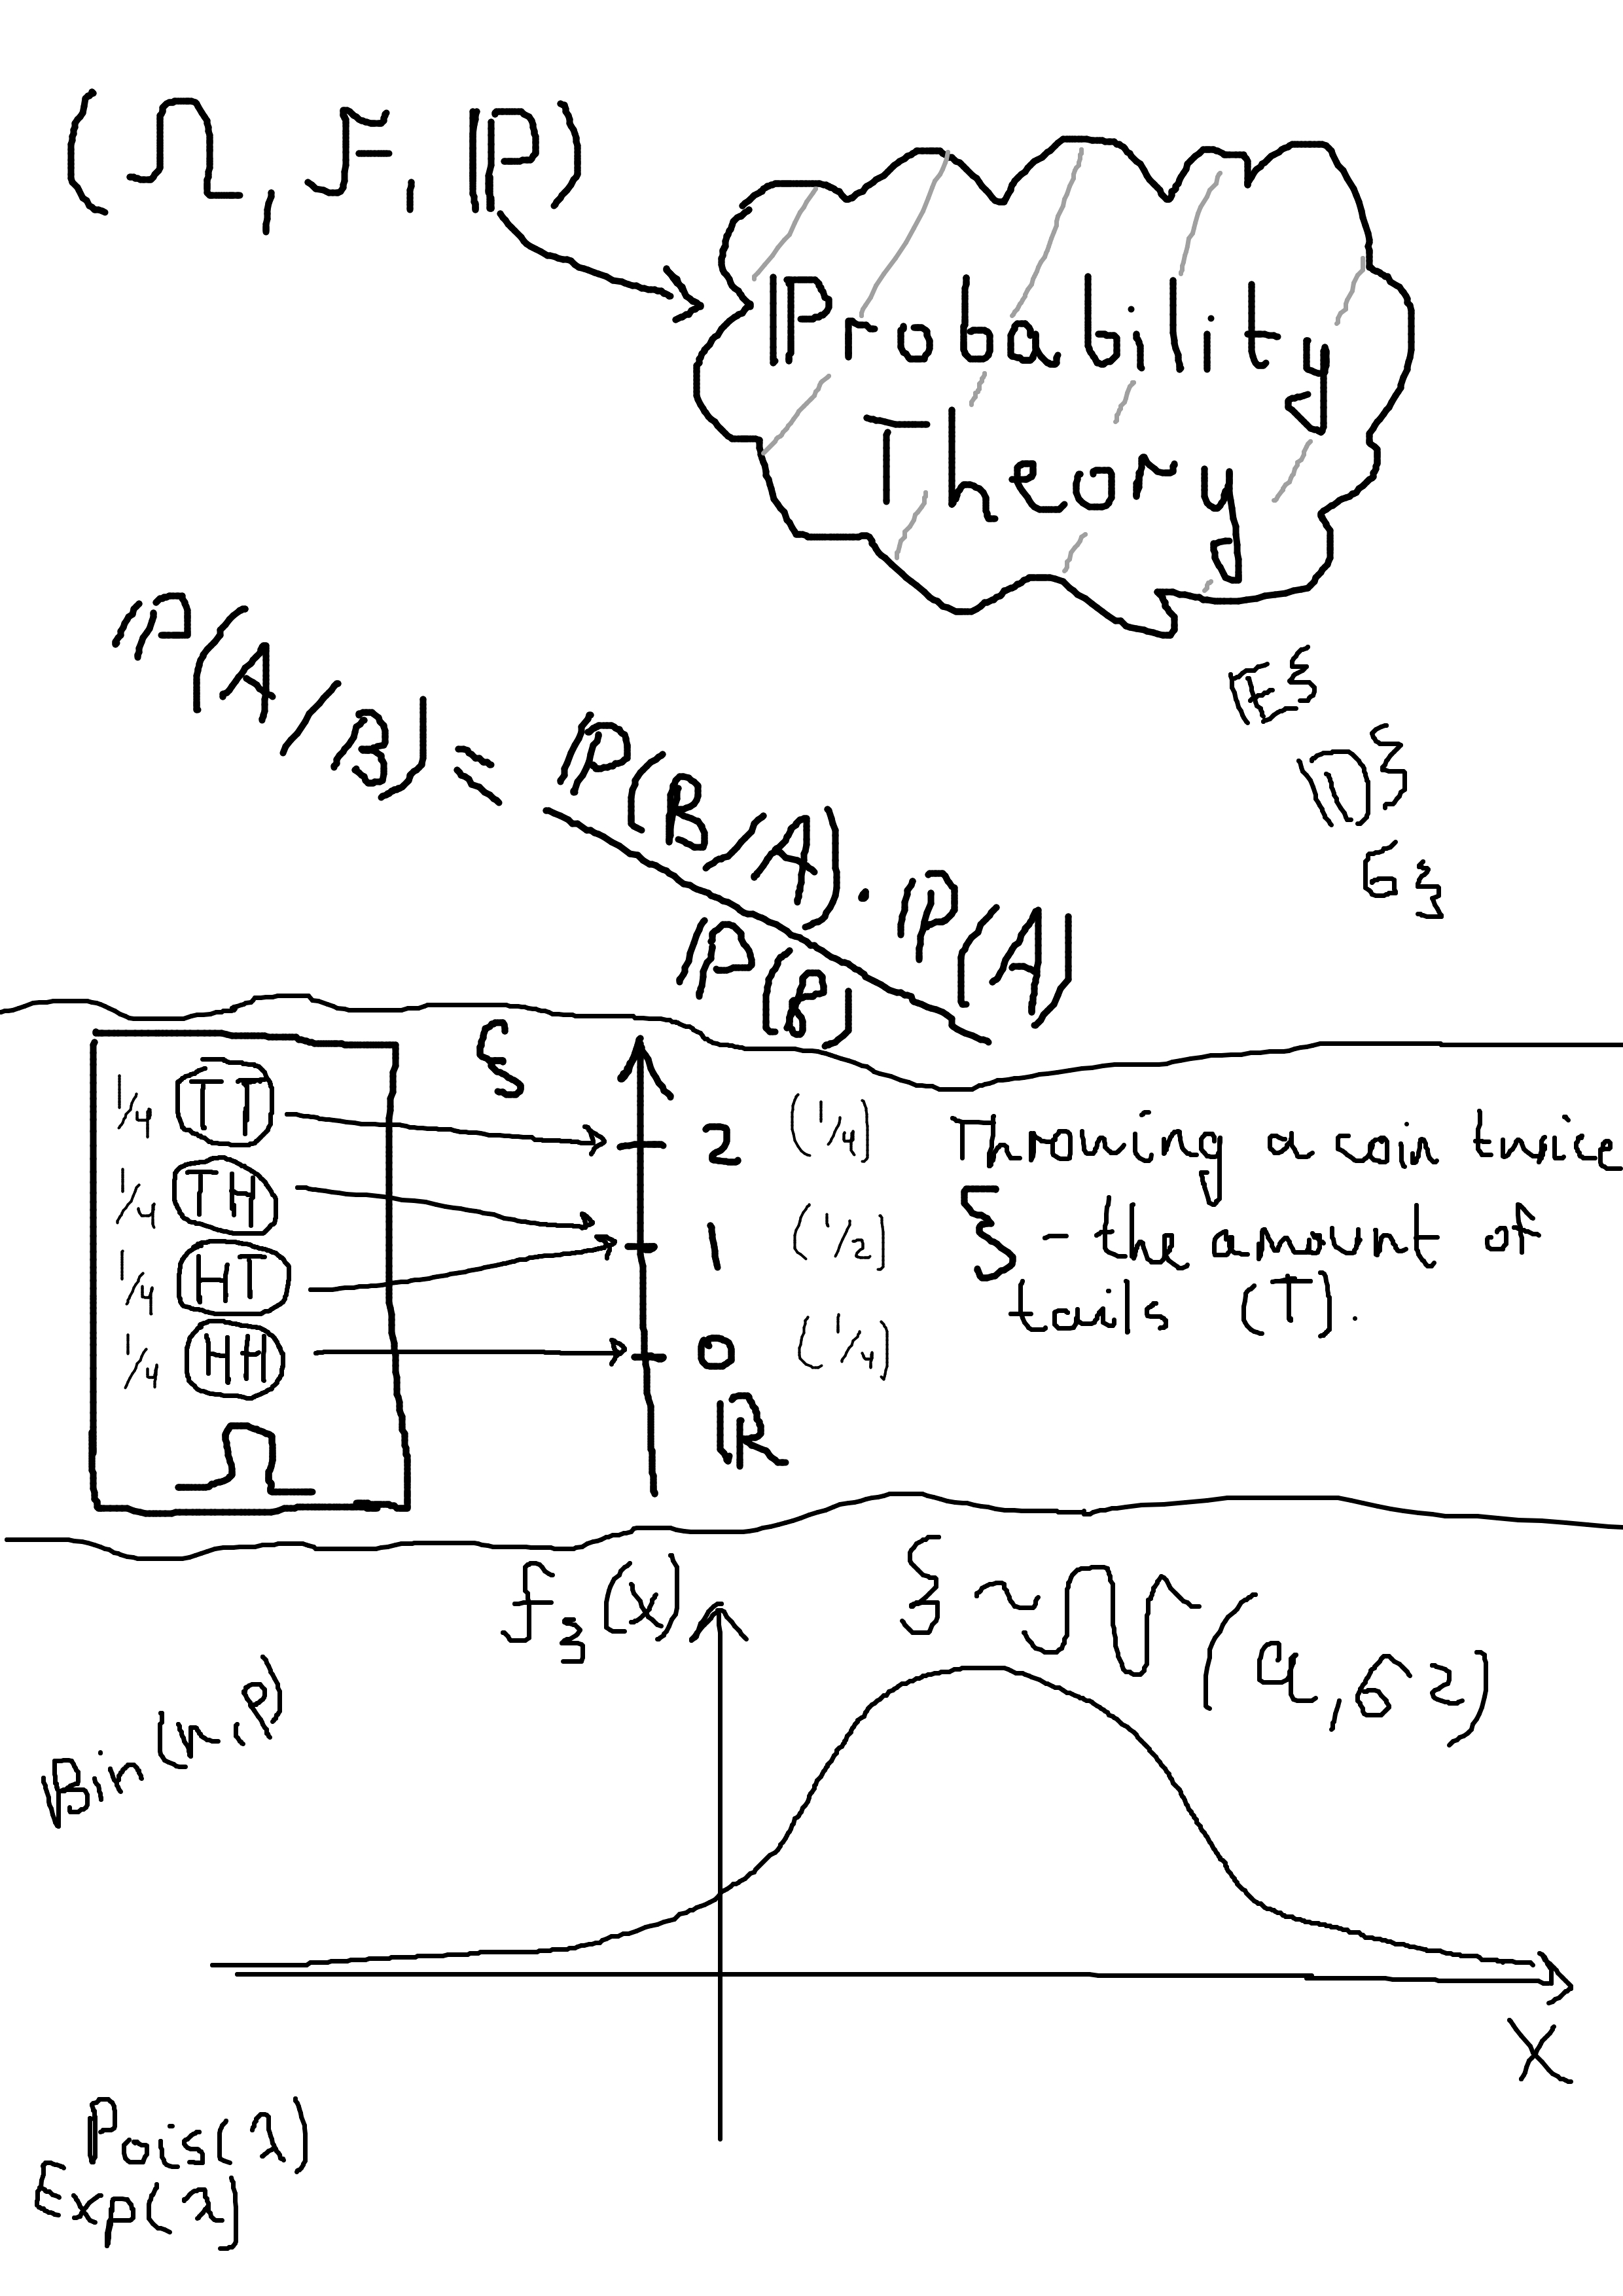
\includepdf{preview.jpg}
\tableofcontents
\newpage
\iffalse
\section{Невизначений інтеграл}
У рамках даного розділу розглядатимуться множини $I,J$, що будуть проміжками одного з типів:\\
$[a,b], (a,b), (a,b]$, причому можливий нескінчений проміжок.
\subsection{Первісна, основні означення невизначеного інтегралу}

\begin{definition}
\textbf{Первісною} для функції $f: I \to \mathbb{R}$ називають функцію $F: I \to \mathbb{R}$, для якої
\begin{align*}
\forall x \in I: F'(x) = f(x)
\end{align*}
\end{definition}

\begin{example}
Зокрема $F(x) = x^2$ - первісна функції $f(x) = 2x$ на $I = \mathbb{R}$.
\end{example}

\begin{example}
Зокрема $F(x) = \begin{cases} 0, & x < 0 \\ \dfrac{x^2}{2}, & x \geq 0\end{cases}$ - первісна функції $f(x) = \begin{cases} 0, & x < 0 \\ x, & x \geq 0 \end{cases}$ на $I = \mathbb{R}$.
\end{example}

\begin{proposition}
Якщо $F(x), \Phi(x)$ - первісні для $f(x)$, то $\Phi(x) = F(x) + C$.\\
\textit{Випливає з наслідків теореми Лагранжа.}
\end{proposition}

\begin{remark}
Не кожна функція може мати первісну. Зокрема $f(x) = \sign x$ не має первісної на $I = [-1,1]$.\\
!Припустимо, що $f$ має первісну $F$, тоді обов'язково $F \in C((-1,1))$. Оберемо $0 < x < 1$ та застосуємо теорему Лагранжа:\\
$F(x) - F(0) = \sign \xi \cdot (x - 0) = x$, де $\xi \in (0,x)$. Таким чином, $\dfrac{F(x)-F(0)}{x} = 1$.\\
При $x \to 0+0$ отримаємо $F'(0+0) = 1$, але водночас $F'(0) = F'(0+0) = 0$. Суперечність!
\end{remark}

\begin{definition}
Множину всіх первісних для функції $f(x)$ називають \textbf{невизначеним інтегралом} функції $f(x)$.\\
Позначення: $\huge \int f(x) \,dx = \{F(x): F'(x) = f(x)\}$.
\end{definition}

\begin{remark}
Але враховуючи твердження вище, ми можемо записувати одну з первісних, тобто \\
$\huge \int f(x) \,dx = F(x) + C$, де $F$ - первісна функції $f$.
\end{remark}

\begin{example}
$\huge\int 2x \,dx = \{x^2 + C | C \in \mathbb{R}\}$.\\
Оскільки є якась первісна, то можна записати як $\huge\int 2x\,dx = x^2 + C$.
\end{example}

\begin{proposition}[Властивості]
1) $\huge \int f'(x)\,dx = f(x) + C$;\\
2) $\huge \left(\int f(x)\,dx \right)' = f(x)$; \\
Далі задамо функції $f,g$, які мають відповідно первісні $F,G$. Тоді:\\
3) $\alpha F$ - первісна для функції $\alpha f$, причому $\huge \int \alpha f(x)\,dx = \alpha \int f(x)\,dx$;\\
4) $F+G$ - первісна для функції $f+g$, причому $\huge \int f(x) + g(x) \,dx = \int f(x)\,dx + \int g(x)\,dx$.
\end{proposition}

\begin{proof}
1), 2) \textit{випливають з означення.} \bigskip \\
3) Якщо $F$ - первісна функції $f$, то тоді $\alpha F$ - первісна функції $\alpha f$, тому що \\ $(\alpha F(x))' = \alpha F'(x) = \alpha f(x)$. \\ Отже, $\huge\int \alpha f(x) \,dx = \alpha F(x) + C = \alpha \left( F(x) + C^* \right) = \alpha \int f(x)\,dx$. \bigskip \\
4) Якщо $F,G$ - первісні відповідно функції $f,g$, то $F+G$ - первісна функції $f+g$, тому що \\ $(F(x)+G(x))' = F'(x)+G'(x) = f(x)+g(x)$. \\ Отже, $\huge\int f(x)+g(x) \,dx = F(x) + G(x) + C = F(x) + C^* + G(x) + C^{**} = \int f(x)\,dx + \int g(x)\,dx$.
\end{proof}

\begin{remark}
Підінтегральний вираз $f(x)\,dx$ варто розглядати як диференціал функції $F(x)$, тобто\\
$\huge\int f(x)\,dx = F(x) + C \iff d(F(x)+C) = f(x)\,dx$
\end{remark}

\begin{remark}
Взагалі-то кажучи, символ $\huge\int f(x)\,dx$ можна також використовувати, щоб позначити як первісну функції $f$, якщо не можна записати $F$ як функцію.\\
Зокрема $\huge\int e^{-x^2}\,dx$ - первісна функції $e^{-x^2}$, проте записати як функцію від змінної не можна.
\end{remark}

\subsubsection*{Таблиця первісних}
\begin{center}
\begin{tabular}{ c|c } 
 $f(x)$ & $F(x)$ \\
 \hline 
 $1$ & $x$ \\ [2ex]
 \hline 
 $x^\alpha$ & $\dfrac{x^{\alpha+1}}{\alpha+1}, \alpha \neq -1$ \\ [2ex]
 \hline
 $\dfrac{1}{x}$ & $\ln |x|$ \\ [2ex]
 \hline
 $\sin x$ & $-\cos x$\\ [2ex]
 \hline 
 $\cos x$ & $\sin x$\\ [2ex]
 \hline
 $\dfrac{1}{\cos^2 x}$ & $\tg x$\\ [2ex]
 \hline 
 $\dfrac{1}{\sin^2 x}$ & $-\ctg x$\\ [2ex]
 \hline
 $\dfrac{1}{\sqrt{1-x^2}}$ & $\arcsin x$\\ [2ex]
 \hline
 $\dfrac{1}{1+x^2}$ & $\arctg x$\\ [2ex]
 \hline
 $\dfrac{1}{\sqrt{1+x^2}}$ & $\ln(x+\sqrt{x^2+1})$\\ [2ex]
 \hline
 $e^x$ & $e^x$ \\ [2ex]
 \hline 
 $a^x$ & $\dfrac{a^x}{\ln a}$ \\ [2ex]
 \hline
 $\sh x$ & $\ch x$ \\ [2ex]
 \hline
 $\ch x$ & $\sh x$ \\ [2ex]
 \hline
 $\dfrac{1}{\ch^2 x}$ & $\th x$\\ [2ex]
 \hline
 $\dfrac{1}{\sh^2 x}$ & $-\cth x$\\
\end{tabular}
\end{center}

\begin{example}
Обчислимо $\huge\int (x+2)^2 + \tg^2 x\,dx$.\\
Робити будемо це, використовуючи таблицю первісних та властивості інтегралів.\\
$\huge\int (x+2)^2 + \tg^2 x\,dx = \int x^2 + 4x + 4 + \dfrac{1}{\cos^2 x} - 1\,dx = \int x^2\,dx + 4 \int x\,dx + 3 \int 1\,dx + \dfrac{1}{\cos^2 x}\,dx = \\ = \dfrac{x^3}{3} + 2x^2 + 3x + \tg x + C$.
\end{example}

\subsection{Заміна змінної}
\begin{theorem} Задано функцію $f: I \to \mathbb{R}$, має первісну $F$; функцію $g: J \to I$ - диференційована. Тоді $(f \circ g) g'$ має первісу $F \circ g$ на $J$, причому \\
$\huge \int (f \circ g)(x) g'(x)\,dx = \int f(t)\,dt$.
\end{theorem}

\begin{proof}
Дійсно, $F \circ g$ - первісна для $(f \circ g) g'$, оскільки $(F \circ g)' (x) = F'(g(x)) g'(x) = f(g(x))g'(x)$. \\
Отже, $\huge \int f(g(x)) g'(x)\,dx = \int f(g(x)) \,dg(x) = \int f(t) \,dt = F(t) + C = F(g(x)) + C$.
\end{proof}

\begin{example} Обчислити $\huge \int \dfrac{1}{x \ln x} \,dx$\\
$\huge \int \dfrac{1}{x \ln x} \,dx \boxed{=} $ \hspace{2cm} Проведемо заміну: $\ln x = t$. Тоді $\dfrac{1}{x}\,dx = dt$\\
$\boxed{=} \huge \int \dfrac{1}{t}\,dt = \ln |t| + C = \ln |\ln x| + C$
\end{example}

\subsection{Інтегрування частинами}
\begin{theorem}
Задані функції $u,v: I \to \mathbb{R}$ - обидва диференційовані. Відомо, що $u'v$ має первісну. Тоді $uv'$ також має первісну, причому\\
$\huge\int u(x)v'(x)\,dx = u(x)v(x) - \int v(x)u'(x)\,dx$.
\end{theorem}

\begin{proof}
Ми знаємо, що $(u(x)v(x))' = u'(x)v(x) + u(x)v'(x) \implies u(x)v'(x) = (u(x)v(x))' - u(x)v'(x)$.\\
Функції $(uv)'$, $uv'$ мають первісну, одна дорівнює $uv$, а інша просто за умовою. Тоді $(uv)' - uv' = uv'$ теж має первісну та дорівнює:\\
$\huge\int u(x)v'(x)\,dx = \int (u(x)v(x))' - u(x)v'(x)\,dx = u(x)v(x) - \int u(x)v'(x)\,dx$.
\end{proof}

\begin{remark}
Більш зручно записати таку формулу: $\huge \int u\,dv = uv - \int v\,du$.
\end{remark}

\begin{example}
Обчислити $\huge \int x^2 e^x \,dx$.\\
$\huge \int x^2 e^x \,dx \boxed{=}$\\
Робимо заміну $u = x^2 \Rightarrow du = 2x\,dx$ \hspace{1cm} $e^x\,dx = dv \Rightarrow v = e^x$\\
$\boxed{=} x^2 e^x - \huge \int 2x e^x\,dx \boxed{\boxed{=}}$\\
Знову заміну $u = 2x \Rightarrow du = 2\,dx$ \hspace{1cm} $e^x\,dx = dv \Rightarrow v = e^x$\\
$\boxed{\boxed{=}} x^2 e^x - (2xe^x - \huge \int 2e^x \,dx) = x^2 e^x - 2xe^x + 2e^x + C$
\end{example}

\subsection{Інтегрування дробово-раціональних функцій}
Розглянемо $\huge \int \dfrac{P(x)}{Q(x)}\,dx$, де $P(x), Q(x)$ - многочлени з дійснийми коефіцієнтами. Є два випадки:\\
I. $\deg(P(x)) \geq \deg(Q(x))$\\
Тоді можемо поділити їх з остачею: $P(x) = S(x)Q(x) + R(x)$.\\
А тому $\huge \int \dfrac{P(x)}{Q(x)}\,dx = \int S(x) + \dfrac{R(x)}{Q(x)}\,dx$\\
,де $S(x)$ - деякий многочлен, який можна проінтегрувати таблицею, а також $\deg(R(x)) < \deg(Q(x))$. Зараз буде пункт, як такий випадок інтегрувати.
\bigskip \\
II. $\deg(R(x)) < \deg(Q(x))$\\
За наслідком основної теореми алгебри, розкладемо $Q(x)$ таким чином: \\
$Q(x) = (x-a_1)^{k_1} \dots (x-a_m)^{k_m} (x^2+p_1x+q_1)^{l_1} (x^2+p_sx+q_s)^{l_s}$. \\
Причому дискримінант квадратних трьохчленів - від'ємний. \\ 
Тоді за теоремою десь із курсу ліналу, ми можемо $\dfrac{R(x)}{Q(x)}$ записати як суму простих дробів:\\
$\dfrac{R(x)}{Q(x)} = \dfrac{A_{11}}{x-a_1} + \dots + \dfrac{A_{1k_1}}{(x-a_1)^{k_1}}+ \dots + \dfrac{A_{m1}}{x-a_m} + \dots + \dfrac{A_{mk_m}}{(x-a_m)^{k_m}} + \\
+ \dfrac{B_{11}x + C_{11}}{x^2+p_1x+q_1} + \dots + \dfrac{B_{1l_1}x + C_{1l_1}}{(x^2+p_1x+q_1)^{l_1}} + \dots + \dfrac{B_{s1}x + C_{s1}}{x^2+p_sx+q_s} + \dots + \dfrac{B_{sl_s}x + C_{sl_s}}{(x^2+p_sx+q_s)^{l_s}}$.\\
Коротше, залишається розглянути 4 вигляди інтегралу:
\bigskip \\
1) $\huge \int \dfrac{A}{x-a}\,dx = A\ln|x-a| + C$
\bigskip \\
2) $\huge \int \dfrac{A}{(x-a)^k}\,dx = A\int (x-a)^{-k}\,dx = A\dfrac{(x-a)^{-k+1}}{-k+1} + C = \dfrac{A}{(1-k)(x-a)^{k-1}} + C$
\bigskip \\
3) $\huge \int \dfrac{Bx+C}{x^2+px+q}\,dx \boxed{=}$\\
Знаменник розпишу як $x^2 + px + q = \left(x + \dfrac{p}{2} \right)^2 + \dfrac{4q-p^2}{4}$.\\
Зробимо заміну: $x + \dfrac{p}{2} = t \Rightarrow dx = dt$\\
Також $Bx+C = Bt - B\dfrac{p}{2} + C$.\\
Перепозначення: $\dfrac{4q-p^2}{4} = a^2 > 0 \hspace{0.5cm} C - B \dfrac{p}{2} = M$.\\
$\boxed{=} \huge \int \dfrac{Bt + M}{t^2 + a^2}\,dt = B \int \dfrac{t}{t^2+a^2}\,dt + M \int \dfrac{1}{t^2+a^2}\,dt \boxed{\boxed{=}}$\\
$\huge \int \dfrac{t}{t^2+a^2}\,dt = \dfrac{dt^2}{2(t^2+a^2)} = \dfrac{1}{2} \ln|t^2+a^2|$\\
$\huge \int \dfrac{1}{t^2+a^2}\,dt = \dfrac{1}{a^2} \int \dfrac{1}{1 + \left(\frac{t}{a}\right)^2}\,dt = \dfrac{1}{a} \int \dfrac{d \frac{t}{a}}{1 + \left(\frac{t}{a}\right)^2} = \dfrac{1}{a} \arctg \dfrac{t}{a}$\\
$\boxed{\boxed{=}} \huge \frac{B}{2} \ln|t^2+a^2| + \frac{M}{a} \arctg \frac{t}{a} + C$\\
Ну а далі робимо зворотню заміну - інтеграл розв'язаний.
\bigskip \\
4) $\huge \int \dfrac{Bx+C}{(x^2+px+q)^l}\,dx \boxed{=}$\\
Тут робимо ті самі заміни, що в 3)\\
$\boxed{=} \huge \int \dfrac{Bt+M}{(t^2+a^2)^l}\,dt = B \int \dfrac{t}{(t^2+a^2)^l} \,dt + M \int \dfrac{1}{(t^2+a^2)^l}\,dt$\\
Ну і тут я ланцюг рівностей зупиню, якщо перший інтеграл - ще ок, то другий - це дупа\\
$\huge \int \dfrac{t}{(t^2+a^2)^l}\,dt = \int \dfrac{dt^2}{2(t^2+a^2)^l}\,dt = \dfrac{1}{2} \dfrac{1}{(1-l)s^{l-1}}$ \bigskip \\
$\huge \int \dfrac{1}{(t^2+a^2)^l}\,dt \boxed{=} \hspace{2cm} u = \dfrac{1}{(t^2+a^2)^l} \hspace{1cm} dv = dt$\\
$\boxed{=} \huge \dfrac{t}{(t^2+a^2)^l} + 2l \int \dfrac{t^2}{(t^2+a^2)^{l+1}}\,dt + \dfrac{t}{(t^2+a^2)^l} + 2l \left(\int \dfrac{dt}{(t^2+a^2)^l} - a^2 \dfrac{dt}{(t^2+a^2)^{l+1}} \right)$\\
Позначимо за $I_l = \huge \int \dfrac{t}{(t^2+a^2)^l}\,dt$\\
Тоді маємо таке рівняння:\\
$I_l = \dfrac{t}{(t^2+a^2)^l} + 2l \cdot I_l - 2la^2 \cdot I_{l+1}$\\
Залишилось виразити $I_{l+1}$ та розв'язати рівняння рекурсивно, причому $I_1$ ми вже рахували.
\bigskip \\
1)+2)+3)+4) $\implies$ інтеграл $\huge\int \dfrac{P(x)}{Q(x)}\,dx$ - розв'язаний.

\begin{example}
Обчислити $\huge \int \dfrac{x^4}{1+x^3}\,dx$\\
Оскільки $\deg(x^4) > \deg(1+x^3)$, то ми поділимо многочлени. Отримаємо:\\
$\huge \int \dfrac{x^4}{1+x^3}\,dx = \int x - \dfrac{x}{x^3+1}\,dx = x^2 - \int \dfrac{x}{x^3+1}\,dx$.\\
Обчислимо другий інтеграл. Перед цим розкладемо дріб на суму простих дробів методом невизначених коефіцієнтів:\\
$\dfrac{x}{x^3+1} = \dfrac{x}{(x+1)(x^2-x+1)} = \dfrac{A}{x+1} + \dfrac{Bx+C}{x^2-x+1} \boxed{=}$\\
$A(x^2-x+1) + (Bx+C)(x+1) = x$\\
$\Rightarrow \begin{cases}
A + B = 0 \\
-A + B + C = 1\\
A + C = 0
\end{cases} \Rightarrow A = -\dfrac{1}{3}, B = \dfrac{1}{3}, C = \dfrac{1}{3}$\\
$\boxed{=} -\dfrac{1}{3(x+1)} + \dfrac{1}{3} \dfrac{x+1}{x^2-x+1}$\\
Таким чином, треба порахувати такий інтеграл:\\
$\huge \int \dfrac{x}{x^3+1}\,dx = -\frac{1}{3} \int \frac{1}{x+1}\,dx + \frac{1}{3} \int \frac{x+1}{x^2-x+1}\,dx \boxed{=}$\\
І розглянемо другий інтеграл:\\
$\huge \int \frac{x+1}{x^2-x+1}\,dx = \int \frac{4x+4}{(2x-1)^2 + 3}\,dx = \int \frac{4x-2}{(2x-1)^2 +3}\,dx + \int \frac{6}{(2x-1)^2 +3}\,dx = \\ = \ln((2x-1)^2+3) + 6 \dfrac{1}{2\sqrt{3}} \arctg \dfrac{2x-1}{\sqrt{3}} = \ln(4x^2-4x+4) + \sqrt{3} \arctg \dfrac{2x-1}{\sqrt{3}}$\\
$\boxed{=} \huge -\dfrac{1}{3} \ln|x+1| + \dfrac{1}{3} \ln(4x^2-4x+4) + \dfrac{1}{\sqrt{3}} \arctg \dfrac{2x-1}{\sqrt{3}}$\\
Разом отримаємо:\\
$\huge \int \dfrac{x^4}{1+x^3}\,dx = x^2 + \dfrac{1}{3} \ln|x+1| - \dfrac{1}{3} \ln(4x^2-4x+4) - \dfrac{1}{\sqrt{3}} \arctg \dfrac{2x-1}{\sqrt{3}} + C$
\end{example}

\begin{example}
Обчислити $\huge\int \dfrac{1}{(x^2+1)^2}\,dx$\\
Можна скористатися отриманою рекурентною формулою, а можна зробити ті самі кроки.\\
$\huge \int \dfrac{1}{(x^2+1)^1}\,dx = \arctg x$\\
$\huge \int \dfrac{1}{(x^2+1)^1}\,dx \overset{u=\text{дріб}, dv = dx}{=} \dfrac{x}{x^2+1} + \int \dfrac{2x^2}{(x^2+1)^2}\,dx = \dfrac{x}{x^2+1} + 2\int \dfrac{1}{x^2+1} - \dfrac{1}{(x^2+1)^2}\,dx$\\
$\implies \huge \arctg x = \dfrac{x}{x^2+1} + 2\arctg x - 2 \int \dfrac{1}{(x^2+1)^2}\,dx$\\
$\huge\int \dfrac{1}{(x^2+1)^2}\,dx = \dfrac{1}{2} \arctg x + \dfrac{x}{2(x^2+1)} + C$
\end{example}

\subsection{Інтегрування тригонометричних функцій}
I. Розглянемо $\huge \int \sin^k x \cos^m x \,dx \hspace{0.5cm}$, де $k,m \in \mathbb{Z}$. Маємо такі заміни:\\
1) $k$ - непарне, тобто $k = 2l+1$, тоді заміна: $\cos x = t$.
\bigskip \\
2) $m$ - непарне, тобто $m = 2l+1$, тоді заміна: $\sin x = t$.
\bigskip \\
3) $k,m$ - парні, тобто $k=2l, m =2n$, тоді знижуємо степені формулами: \\ $\sin^2 x = \dfrac{1-\cos 2x}{2} \hspace{0.5cm} \cos^2 x = \dfrac{1+\cos 2x}{2}$.
\bigskip \\
Всі ці заміни приведуть до інтегрування дробово-раціональних виразів.

\begin{example}
Обчислити $\huge\int \cos^3 x \,dx$\\
Заміна: $t = \sin x$, випадок 2), тоді $dt = \cos x \,dx$\\
$\huge\int \cos^3 x \,dx = \int (1-t^2)\,dx = t - \dfrac{t^3}{3} + C = \sin x - \dfrac{\sin^3 x}{3} + C$
\end{example}

II. Розглянемо $\huge \int R(\sin x, \cos x)\,dx \hspace{0.5cm}$, де $R$ - дробово-раціональний вираз від $\sin x, \cos x$. Маємо таку заміну - її ще називають \textbf{універсальною тригонометричною підстановкою}:\\
$t = \tg \dfrac{x}{2} \implies x = 2 \arctg t \implies dx = \dfrac{2}{1+t^2}\,dt$\\
$\sin x = \dfrac{2 \tg \frac{x}{2}}{1 + \tg^2 \frac{x}{2}} = \dfrac{2t}{1+t^2}$\\
$\cos x = \dfrac{1 - \tg^2 \frac{x}{2}}{1 + \tg^2 \frac{x}{2}} = \dfrac{1-t^2}{1+t^2}$.\\
Підставивши, ми отримуємо випадок інтегрування дробово-раціональних виразів.

\begin{example}
Обчислити $\huge \int \dfrac{dx}{5-3\cos x}$\\
Заміна: $t = \tg \dfrac{x}{2}$, випадок II. Тоді беремо решта замін звідси, з нашого пункту.\\
$\huge \int \dfrac{dx}{5-3\cos x} = \int \dfrac{1}{5-3 \frac{1-t^2}{1+t^2}} \dfrac{2}{1+t^2}\,dt = \int \dfrac{2\,dt}{5+5t^2-3+3t^2} = \int \dfrac{dt}{4t^2+1} = \dfrac{1}{2} \arctg 2t + C = \\ = \dfrac{1}{2} \arctg \left(2 \tg \dfrac{x}{2} \right) + C$
\end{example}
Але універсальна підстановка не завжди може буде ефективною.\\
III. Проводжимо розглядати $\huge\int R(\sin x, \cos x) \,dx$. Нехай є кілька випадків:\\
1) $R(-u,v) = -R(u,v)$, тоді заміна: $\cos x = t$;\\
2) $R(u,-v) = -R(u,v)$, тоді заміна: $\sin x = t$;\\
3) $R(-u,-v) = R(u,v)$, тоді заміна: $\tg x = t$ або $\ctg x = t$.\\
\textit{Без доведення. Важкі алгебраїчні перетворення.}

\begin{example}
Обчислити $\huge\int \dfrac{1}{(2+\cos x) \sin x}\,dx$.\\
Маємо $R(\sin x,\cos x) = \dfrac{1}{(2+\cos x)\sin x}$, зауважимо, що $R(-\sin x, \cos x) = -R(\sin x, \cos x)$, тож беремо заміну $t = \cos x$. Отже,\\
$\huge\int \dfrac{1}{(2+\cos x) \sin x}\,dx = \int \dfrac{1}{(2+t)(1-t^2)}\,dt = \dots = \dfrac{1}{3} \ln |t+2| - \dfrac{1}{2} \ln |t+1| + \dfrac{1}{6} \ln |t-1| + C = \\ = \dfrac{1}{3} \ln |\cos x + 2| - \dfrac{1}{2} \ln |\cos x +1| + \dfrac{1}{6} \ln | \cos x - 1| + C$.
\end{example}
\subsection{Інтегрування ірраціональних виразів}

I. Розглянемо $\huge \int R\left( \sqrt[k_1]{\dfrac{ax+b}{cx+d}}, \dots, \sqrt[k_n]{\dfrac{ax+b}{cx+d}} \right)\,dx$, де $R$ - дробово-раціональний вираз, причому $ad-cb \neq 0$.\\
Заміна: $\dfrac{ax+b}{cx+d} = t^m$, де число $m = \text{lcm}(k_1,\dots,k_n)$.\\
Виразимо $x$ з цього рівняння:\\
$ax+b =t^m cx + t^m d \implies x = \dfrac{t^md-b}{a-ct^m}$\\
А потім шукаємо $dx = \dfrac{mt^{m-1}(ad-bc)}{(a-ct)^2}\,dt$.\\
Підставивши, ми отримуємо інтеграл дробово-раціонального виразу.

\begin{example}
Обчислити $\huge \int \dfrac{\sqrt{x+1}+2}{(x+1)^2 - \sqrt{x+1}}\,dx$\\
Заміна: $t^2 = x+1$. Тоді $x = t^2 -1 \Rightarrow dx = 2t \,dt$\\
$\huge \int \dfrac{\sqrt{x+1}+2}{(x+1)^2 - \sqrt{x+1}}\,dx = \int \dfrac{t+2}{t^4-t} \cdot 2t\,dt = 2 \int \dfrac{t+2}{t^3-1}\,dt \boxed{=}$\\
обчислення цього інтегралу проводиться як в п. 4, тому я пропускаю цей момент\\
$\boxed{=} -\ln(t^2+t+1) - \dfrac{2}{\sqrt{3}} \arctg \dfrac{2t+1}{\sqrt{3}} + 2 \ln|t-1|+ C = \\
= -\ln(x+2+\sqrt{x+1}) - \dfrac{2}{\sqrt{3}} \arctg \dfrac{2\sqrt{x+1}+1}{\sqrt{3}} + 2 \ln|\sqrt{x+1}-1| + C$
\end{example}

II. Розглянемо такі інтеграли:\\
1) $\huge \int R(x,\sqrt{a^2-x^2})\,dx$\\
Заміна: $x = a\sin t \Rightarrow dx = a\cos t \,dt$
\bigskip \\

2) $\huge \int R(x,\sqrt{a^2+x^2})\,dx$\\
Заміна: $x = a\tg t \Rightarrow dx = \dfrac{a}{\cos^2 t} dt$\bigskip \\

\iffalse
Або інша заміна: $x = a \sh t \Rightarrow dx = a \ch t \,dt$\\
$\boxed{=} \huge \int R(a\sh t, a \ch t) \cdot a \ch t\,dt$
\bigskip \\
\fi

3) $\huge \int R(x, \sqrt{x^2-a^2})\,dx$\\
Заміна: $x = \dfrac{a}{\cos t} \Rightarrow dx = \dfrac{a}{\cos^2 t} \sin t\,dt$\\

\iffalse
Або інша заміна: $x = a \ch t \Rightarrow dx = a \sh t \,dt$\\
$\boxed{=} \huge \int R(a \ch t, a \sh t) \cdot a \sh t \,dt$
\bigskip \\
\fi
Усі заміни приведуть до інтегралу тригонометричних функцій.

\begin{example}
Обчислити $\huge \int \sqrt{4-x^2}\,dx$\\
Заміна: $x = 2\sin t$, випадок 1). Тоді $dx = 2 \cos t \,dt$\\
$\huge \int \sqrt{4-x^2}\,dx = \int 2 \cos t \cdot 2 \cos t \,dt = \int 2(1+\cos 2t)\,dt = 2t + \sin 2t + C = 2t + 2 \sin t \cos t + C = \\ = 2 \arcsin \frac{x}{2} + 2 \frac{x}{2} \sqrt{1-\frac{x^2}{4}}+C = 2 \arcsin \frac{x}{2} + \dfrac{x \sqrt{4-x^2}}{2} + C$
\end{example}

\subsection{Диференціальний біном}
Розглянемо $\huge \int x^m (ax^n + b)^p\,dx \hspace{1cm}$, де $m,n,p \in \mathbb{Q}$. Існують лише три випадки, як його розв'язати, для цього я наведу діаграму нижче, які застосовувати заміни.\\
Але для початку оскільки $m,n,p \in \mathbb{Q}$, то я запишу як дріб $m= \dfrac{s_1}{q_1},\hspace{1cm} n = \dfrac{s_2}{q_2},\hspace{1cm} p = \dfrac{s_3}{q_3}$.\\
\begin{tikzcd}
p \in \mathbb{Z} \arrow{r}{\text{ні}} \arrow{d}{\text{так}} & \dfrac{m+1}{n} \in \mathbb{Z} \arrow{d}{\text{так}} \arrow{r}{\text{ні}} & p+\dfrac{m+1}{n} \in \mathbb{Z} \arrow{d}{\text{так}} \arrow{r}{\text{ні}} & \textbf{не обчислюється} \\
x = t^{\text{lcm}(q_1,q_2)} & ax^n+b=t^{q_3} & a+bx^{-n} = t^{q_3} &
\end{tikzcd}\\

\iffalse
1) $p \in \mathbb{Z}$, тоді числа $m,n$ подамо в вигляді дробу: \\
$m = \dfrac{p_1}{q_1}; n = \dfrac{p_2}{q_2}$.\\
Встановимо $q = \textrm{LCM}(q_1,q_2)$. Тоді заміна: $x = t^q$.
\bigskip \\
2) $p \not \in \mathbb{Z}$, але $\dfrac{m+1}{n} \in \mathbb{Z}$, тоді число $p$ подамо в вигляді дробу:\\
$p = \dfrac{j}{l}$.\\
Тоді заміна: $ax^n+b = t^l$.
\bigskip \\
3) $p \not \in \mathbb{Z}$ та $\dfrac{m+1}{n} \not \in \mathbb{Z}$, але $p+ \dfrac{m+1}{n} \in \mathbb{Z}$, тоді число $p$ подамо в вигляді дробу:\\
$p = \dfrac{j}{l}$.\\
Тоді заміна: $a+bx^{-n} = t^l$.
\bigskip \\
\fi
Заміни називають \textbf{підстановками Чебишова}, що приводять до інтегралу дробово-раціональних виразів. Якщо жодна з пунктів не спрацьовує, то інтеграл не може бути обчисленим через елементарні функції (\textit{без доведення}).
\begin{example}
Обчислити $\huge \int \sqrt[3]{x-x^3}\,dx = \int x^{\frac{1}{3}} (1-x^2)^\frac{1}{3}\,dx$\\
Тут у нас $m = \dfrac{1}{3}$, $n = 2$, $p = \dfrac{1}{3}$\\
Спрацьовує 3), тому що $p + \dfrac{m+1}{n} = \dfrac{1}{3} + \dfrac{1+\frac{1}{3}}{2} = 1 \in \mathbb{Z}$\\
Заміна: $-1+x^{-2}=t^3$\\
$-2x^{-3}\,dx = 3t^2\,dt$\\
$\huge \int \sqrt[3]{x-x^3}\,dx = \int x^{\frac{1}{3}} (1-x^2)^\frac{1}{3}\,dx = \int (x^{-2}-1)^{\frac{1}{3}} x^{\frac{2}{3}} x^{\frac{1}{3}}\,dx = \int t \cdot x \cdot \frac{3t^2 x^3 \,dt}{-2} = \int \frac{3t^3\,dt}{-2(t^3+1)^2} = \\ = \frac{3}{-2} \left(\int \frac{dt}{t^3+1} - \int \frac{dt}{(t^3+1)^2} \right) \boxed{=}
$\\
обчислення цього інтегралу проводиться як в п. 4, тому я пропускаю цей момент\\
$\boxed{=} \huge -\frac{\ln|t+1|}{2} + \frac{\ln(t^2-t+1)}{4} - \frac{\sqrt{3}}{2} \arctg \frac{2x-1}{\sqrt{3}} + \frac{\ln |t+1|}{3} - \frac{\ln(t^2-t+1)}{6} + \frac{\sqrt{3}}{3} \arctg \frac{2x-1}{\sqrt{3}} + \frac{t}{2t^3+2} + C =\\
= - \frac{1}{6} \ln|t+1| + \frac{1}{12} \ln(t^2-t+1) - \frac{\sqrt{3}}{6} \arctg \frac{2x-1}{\sqrt{3}} + \frac{t}{2t^3+2} + C$\\
І підставляємо $t = \sqrt[3]{x^{-2}+1}$.
\end{example}

\newpage
\fi

\iffalse
\section{Визначений інтеграл}
\subsection{Підхід Рімана}
\begin{definition}
\textbf{Розбиттям} множини $[a,b]$ називають множину точок $\tau = \{x_0,x_1,\dots,x_{n-1},x_n\}$ при $n \in \mathbb{N}$, для яких
\begin{align*}
a = x_0 < x_1 < \dots < x_{n-1} < x_{n} = b
\end{align*}
\end{definition}

\begin{definition}
Позначимо за $\Delta x_1 = x_1 - x_0, \dots, \Delta x_n = x_{n} - x_{n-1}$. Тоді число
\begin{align*}
|\tau| = \max\{\Delta x_1,\dots, \Delta x_n\}
\end{align*}
називають \textbf{діаметром} (або \textbf{дрібністю}) розбиття $\tau$.
\end{definition}

\begin{definition}
Задані розбиття $\tau, \tau'$ відрізка $[a,b]$.\\
$\tau'$ називають \textbf{підрозбиттям} розбиття $\tau$, якщо
\begin{align*}
\tau \subset \tau'.
\end{align*}
\end{definition}

\begin{proposition}
Задано $\tau'$ -- підрозбиття для $\tau$. Тоді $|\tau'| \leq |\tau|$.
\end{proposition}

\begin{proof}
Із розбиття ми можемо отримати підрозбиття шляхом додавання точок. Тоді деякі інтервали будуть ділитись на підінтервали через додавання точки. Відповідно діаметр зменшується.
\end{proof}

\begin{definition}
Задано $\tau = \{x_0,x_1,\dots,x_n\}$ - розбиття відрізка $[a,b]$.\\
Елементи множини $\xi = \{\xi_1, \dots, \xi_n \}$ називають \textbf{відміченими точками}. Для них
\begin{align*}
\xi_1 \in [x_0,x_1),\ \xi_2 \in [x_1,x_2),\ \dots,\ \xi_n \in [x_{n-1}, x_n].
\end{align*}
\end{definition}

\begin{definition}
Задано функцію $f \colon [a,b] \to \mathbb{R}$, розбиття $\tau = \{x_0,x_1,\dots,x_n\}$ та відмічені точки $\xi = \{\xi_1, \dots, \xi_n \}$.\\
\textbf{Інтегральною сумою Рімана} функції $f$ для нашого розбиття $\tau$ та відмічених точок називають число:
\begin{align*}
\sigma (f, \tau, \xi) = \sum_{k=1}^n f(\xi_k) \Delta x_k
\end{align*}
\end{definition}

\begin{figure}[H]
\centering
\begin{tikzpicture}
\draw[thick] (1,-1pt)--(1,1pt) node[anchor = north] {$x_0$};
\draw[thick] (2,-1pt)--(2,1pt) node[anchor = north] {$x_1$};
\draw[thick] (4,-1pt)--(4,1pt) node[anchor = north east] {$x_{n-1}$};
\draw[thick] (5,-1pt)--(5,1pt) node[anchor = north] {$x_n$};


\draw[fill = black!30] (1,0) rectangle (2, {exp((1.5-2)/3)});
\draw[fill = black!30] (4,0) rectangle (5, {exp((4.5-2)/3)});

\draw[thick, dashed] (1.5,{exp((1.5-2)/3)})--(1.5,0) node[anchor = north, scale = 0.8] {$\xi_1$};
\draw[thick, dashed] (4.5,{exp((4.5-2)/3)})--(4.5,0) node[anchor = north, scale = 0.8] {$\xi_n$};

\draw[thick, ->] (-0.5,0)--(5.5,0) node[anchor = north] {$x$};
\draw[thick, ->] (0,-0.5)--(0,3) node[anchor = east] {$y$};

\draw[thick, domain=1:5, variable=\x, samples = 1000] plot({\x}, {exp((\x-2)/3)});
%node[anchor = south east, scale = 0.8] {$f(x) = \dfrac{\sin x}{x}$};
%\node[white] at (0,1) [circle,fill,inner sep=1.5pt, draw = black]{};
%\node[black] at (0,0) [circle,fill,inner sep=1.5pt, draw = black]{};
\end{tikzpicture}
\end{figure}

\begin{definition}
Задано функцію $f \colon [a,b] \to \mathbb{R}$.\\
Функція $f$ називається \textbf{інтегрованою за Ріманом} на $[a,b]$, якщо існує таке число $I \in \mathbb{R}$, для якого виконана умова:
\begin{align*}
\forall \varepsilon > 0: \exists \delta(\varepsilon) > 0: \forall (\tau, \xi): |\tau| < \delta \implies \abs{\sigma(\tau, \xi, f) - I} < \varepsilon
\end{align*}
Число $I$ називають \textbf{інтегралом Рімана}.
\begin{align*}
I = \int_a^b f(x)\,dx
\end{align*}
Позначення: $I = \huge\lim_{|\tau| \to 0} \sigma(f, \tau, \xi)$ \iffalse(трошки нелегально, тому що не знаю, що таке границя за базою).\fi \\ 
Множина інтегрованих функцій за Ріманом позначається так: $\mathcal{R}([a,b])$.
\end{definition}

\begin{remark}
Детально переформулюю частину означення: для кожного розбиття $\tau$, якщо вона є скільки завгодно малою, то тоді виконується нерівність для кожної множини обраних точок $\xi$.\\
Також нотація $\huge\lim_{|\tau| \to 0} \sigma(f,\tau,\xi)$ -- це не границя функції $\sigma$ в звичному вигляді, а трохи іншої специфікації границя.
\end{remark}

\begin{example}
Доведемо, що функція $f(x) = 1 \in \mathcal{R}([a,b])$, а також $\huge \int_a^b 1\,dx = b-a$.\\
Для початку зафіксуємо розбиття $\tau = \{x_0,x_1,\dots,x_n\}$ та відмітимо точки $\xi = \{\xi_1,\dots,\xi_n\}$. Це аби знайти інтегральну суму:\\
$\sigma (f, \tau, \xi) = \huge \sum_{k=1}^n f(\xi_k) \Delta x_k$\\
$\sigma (1, \tau, \xi) = \huge \sum_{k=1}^n \Delta x_k = x_1 - x_0 + x_2 - x_1 + \dots + x_n - x_{n-1} = x_n - x_0 = b - a$.\\
Інтегральна сума має це значенням при довільному розбитті. Якщо встановити $I = b -a$, то:\\
$\forall \varepsilon > 0: \exists \delta(\varepsilon) > 0: \forall (\tau, \xi): |\tau| < \delta \implies |\sigma (\tau, \xi, f) - I| = |b-a - (b-a)| = 0 < \varepsilon$.\\
Отже, $f(x) = 1 \in \mathcal{R}([a,b])$, а інтеграл $\huge \int_a^b 1\,dx = b-a$.
\end{example}

\begin{theorem}
Задано функцію $f \colon [a,b] \to \mathbb{R}$.\\
Число $I$ -- інтеграл Рімана $\iff \forall (\tau_n, \xi_n): |\tau_n| \overset{n \to \infty}{\longrightarrow} 0 \implies \sigma(f, \tau_n, \xi_n) \overset{n \to \infty}{\longrightarrow} I$.\\
\textit{Зрозуміло. Фактично, це можна вважати як означення 'за Гайне', але не зовсім. Проте схожі.}
\end{theorem}

Підхід Рімана, на жаль, зовсім незручний для побудови теорії. Тому треба еквівалентні підходи.

\subsection{Суми Дарбу}
\begin{definition}
Задано функцію $f \colon [a,b] \to \mathbb{R}$ -- обмежена. Визначмо такі значення для розбиття $\tau = \{x_0,x_1,\dots,x_n\}$:
\begin{align*}
m_k = \inf_{x \in [x_{k-1},x_k]} f(x) \hspace{2cm} M_k = \sup_{x \in [x_{k-1},x_k]} f(x) \hspace{0.5cm} k=1,\dots,n
\end{align*}
\textbf{Верхньою та нижньою сумою Дарбу} називають такі суми:
\begin{align*}
U(f, \tau) = \sum_{k=1}^n M_k \Delta x_k \hspace{2cm} L(f,\tau) = \sum_{k=1}^n m_k \Delta x_k \hspace{2cm}
\end{align*}
\end{definition}
\begin{figure}[H]
\centering
\begin{tikzpicture}
\draw[thick] (1,-1pt)--(1,1pt) node[anchor = north] {$x_0$};
\draw[thick] (2,-1pt)--(2,1pt) node[anchor = north] {$x_1$};
\draw[thick] (5,-1pt)--(5,1pt) node[anchor = north] {$x_n$};
\foreach \i in {1,2,3,4}
	\draw[fill = black!30] (\i,0) rectangle (\i+1, {exp((\i-1)/3)});

\draw[thick, ->] (-0.5,0)--(5.5,0) node[anchor = north] {$x$};
\draw[thick, ->] (0,-0.5)--(0,3) node[anchor = east] {$y$};

\draw[thick, domain=1:5, variable=\x, samples = 1000] plot({\x}, {exp((\x-2)/3)});
\node at (1,2) {$U(f,\tau)$};
\end{tikzpicture}
\qquad
\begin{tikzpicture}
\draw[thick] (1,-1pt)--(1,1pt) node[anchor = north] {$x_0$};
\draw[thick] (2,-1pt)--(2,1pt) node[anchor = north] {$x_1$};
\draw[thick] (5,-1pt)--(5,1pt) node[anchor = north] {$x_n$};
\foreach \i in {1,2,3,4}
	\draw[fill = black!30] (\i,0) rectangle (\i+1, {exp((\i-2)/3)});

\draw[thick, ->] (-0.5,0)--(5.5,0) node[anchor = north] {$x$};
\draw[thick, ->] (0,-0.5)--(0,3) node[anchor = east] {$y$};

\draw[thick, domain=1:5, variable=\x, samples = 1000] plot({\x}, {exp((\x-2)/3)});
\node at (1,2) {$L(f,\tau)$};
\end{tikzpicture}
\end{figure}

\begin{remark}
Із означення випливає, що $L(f,\tau) \leq \sigma(f,\tau,\xi) \leq U(f,\tau)$, оскільки $m_k \leq f(\xi_k) \leq M_k$.
\end{remark}

\begin{lemma}
Задано функцію $f \colon [a,b] \to \mathbb{R}$ -- обмежена та будь-яке розбиття $\tau$. Тоді маємо:\\
$L(f,\tau) = \huge\inf_{\xi} \sigma(f,\tau,\xi) \hspace{1cm} U(f,\tau) = \huge\sup_{\xi} \sigma(f,\tau,\xi)$
\end{lemma}

\begin{proof}
Зафіксуємо розбиття $\tau = \{x_0,x_1,\dots,x_n\}$, тоді $f$ -- обмежена на $[x_{k-1},x_k], \forall k$.\\
А тепер візьмемо деякий набір точок $\xi$, тоді зрозуміло, що $f(\xi_k) \leq M_k, \forall k \implies f(\xi_k) \Delta x_k \leq M_k \Delta x_k$.\\
Просумуємо всі рівняння, які тут в нас є -- тоді отримаємо:\\
$\huge\sum_{k=1}^n f(\xi_k) \Delta x_k \leq \huge\sum_{k=1}^n M_k \Delta x_k \implies \sigma(f,\tau,\xi) \leq U(f, \tau)$.
\bigskip \\
А далі зафіксуємо $\varepsilon > 0$. Оскільки $M_k = \huge\sup_{x \in [x_{k-1},x_k]} f(x)$, то тоді $\exists x_\varepsilon: f(x_\varepsilon) > M_k - \dfrac{\varepsilon}{b-a}$.\\
І ось ці точки $x_\varepsilon = \xi_k'$ - це буде мій набір точок, який існує. Тоді маємо\\
$f(\xi_k') > M_k - \dfrac{\varepsilon}{b-a} \implies f(\xi_k') \Delta x_k > M_k \Delta x_k - \dfrac{\varepsilon}{b-a} \Delta x_k$\\
Аналогічно просумуємо всі рівняння -- отримаємо:\\
$\huge\sum_{k=1}^n f(\xi_k') \Delta x_k > \sum_{k=1}^n M_k \Delta x_k - \sum_{k=1}^n \dfrac{\varepsilon}{b-a} \Delta x_k \implies S_{\tau, \xi'}(f) > U(f,\tau) - \varepsilon$.\\
Остаточно, ми отримали $U(f, \tau) = \huge\sup_\xi \sigma(f,\tau,\xi)$. Випадок $L(f,\tau) = \huge\inf_\xi \sigma(f,\tau,\xi)$ аналогічний.
\end{proof}

\begin{lemma}
Задано функцію $f \colon [a,b] \to \mathbb{R}$ -- обмежена та розбиття $\tau$. Також задамо підрозбитя $\tau'$. Тоді $U(f,\tau) \geq U(f,\tau')$, а також $L(f,\tau) \leq L(f,\tau')$.
\end{lemma}

\begin{figure}[H]
\centering
\begin{tikzpicture}

\foreach \i in {1,2,3,4}
	\draw[fill = black!30] (\i,0) rectangle (\i+1, {exp((\i-1)/3)});

\draw[thick, ->] (-0.5,0)--(5.5,0) node[anchor = north] {$x$};
\draw[thick, ->] (0,-0.5)--(0,3) node[anchor = east] {$y$};

\draw[thick, domain=1:5, variable=\x, samples = 1000] plot({\x}, {exp((\x-2)/3)});
\node at (1,2) {$U(f,\tau)$};
\end{tikzpicture}
\qquad
\begin{tikzpicture}

\foreach \i in {1,1.5,2,2.5,3,3.5,4,4.5}
	\draw[fill = black!30] (\i,0) rectangle (\i+0.5, {exp((\i-1.5)/3)});

\draw[thick, ->] (-0.5,0)--(5.5,0) node[anchor = north] {$x$};
\draw[thick, ->] (0,-0.5)--(0,3) node[anchor = east] {$y$};

\draw[thick, domain=1:5, variable=\x, samples = 1000] plot({\x}, {exp((\x-2)/3)});
\node at (1,2) {$U(f,\tau')$};
\end{tikzpicture}
\end{figure}

\begin{figure}[H]
\centering
\begin{tikzpicture}

\foreach \i in {1,2,3,4}
	\draw[fill = black!30] (\i,0) rectangle (\i+1, {exp((\i-2)/3)});

\draw[thick, ->] (-0.5,0)--(5.5,0) node[anchor = north] {$x$};
\draw[thick, ->] (0,-0.5)--(0,3) node[anchor = east] {$y$};

\draw[thick, domain=1:5, variable=\x, samples = 1000] plot({\x}, {exp((\x-2)/3)});
\node at (1,2) {$L(f,\tau)$};
\end{tikzpicture}
\qquad
\begin{tikzpicture}

\foreach \i in {1,1.5,2,2.5,3,3.5,4,4.5}
	\draw[fill = black!30] (\i,0) rectangle (\i+0.5, {exp((\i-2)/3)});

\draw[thick, ->] (-0.5,0)--(5.5,0) node[anchor = north] {$x$};
\draw[thick, ->] (0,-0.5)--(0,3) node[anchor = east] {$y$};

\draw[thick, domain=1:5, variable=\x, samples = 1000] plot({\x}, {exp((\x-2)/3)});
\node at (1,2) {$L(f,\tau')$};
\end{tikzpicture}
\end{figure}

\begin{proof}
Достатньо розглянути підрозбиття $\tau' = \tau \cup \{x^*\}$, припустимо $x^* \in [x_{i-1},x_i], i = \overline{1,n}$. Тому що якщо в мене буде більше точок, то будемо поступово їх додавати.\\
$U(f,\tau) = \huge\sum_{k=1}^n M_k \Delta x_k = M_i \Delta x_i + \sum_{k=1, k \neq i}^n M_k \Delta x_k \boxed{\geq}$\\
Зауважимо, що виконується така нерівність:\\
$M_i \Delta x_i = M_i (x_i - x_{i-1}) = M_i (x_i - x^* + x^* - x_{i-1}) = M_i (x_i - x^*) + M_i (x^* - x_{i-1}) \geq \\ \geq \widetilde{M} (x_i-x^*) + \widetilde{\widetilde{M}}(x^*-x_{i-1})$, де $\widetilde{M} = \huge\sup_{x \in [x^*, x_i] } f(x), \quad \widetilde{\widetilde{M}} = \huge\sup_{x \in [x_{i-1}, x^*] } f(x)$.
\begin{figure}[H]
\centering
\begin{tikzpicture}[scale = 1.5]
\draw[thick, ->] (0.5,0)--(3.5,0) node[anchor = north] {$x$};

\draw[fill = black!30] (1.5,0) rectangle (2.8, 1);
\draw[thick, domain=1.5:2.8, variable=\x, samples = 1000] plot({\x}, {-(\x-2)^2+1});
\draw (1.5,1pt)--(1.5,-1pt) node[anchor = north] {$x_{i-1}$};
\draw (2.8,1pt)--(2.8,-1pt) node[anchor = north] {$x_{i}$};
\end{tikzpicture}
\qquad
\begin{tikzpicture}[scale = 1.5]
\draw[thick, ->] (0.5,0)--(3.5,0) node[anchor = north] {$x$};

\draw[fill = black!30] (1.5,0) rectangle (2.3, 1);
\draw[fill = black!30] (2.3,0) rectangle (2.8, {-(2.3-2)^2+1});
\draw[thick, domain=1.5:2.8, variable=\x, samples = 1000] plot({\x}, {-(\x-2)^2+1});
\draw (1.5,1pt)--(1.5,-1pt) node[anchor = north] {$x_{i-1}$};
\draw (2.8,1pt)--(2.8,-1pt) node[anchor = north] {$x_{i}$};
\draw (2.3,1pt)--(2.3,-1pt) node[anchor = north] {$x^*$};
\end{tikzpicture}
\end{figure}
$\boxed{\geq} \huge\sum_{k=1, k \neq i}^n M_k \Delta x_k + \widetilde{M} (x_i - x^*) + \widetilde{\widetilde{M}} (x^* - x_{i-1}) = U(f, \tau \cup \{x^*\}) = U(f,\tau')$.\\
Випадок $L(f,\tau) \leq L(f,\tau')$ аналогічний.
\end{proof}

\begin{lemma}
Задано функцію $f \colon [a,b] \to \mathbb{R}$ -- обмежена. Візьмемо будь-які два розбиття $\tau', \tau''$. Тоді $L(f,\tau') \leq U(f,\tau'')$.
\end{lemma}

\begin{proof}
Зафіксую $\tau = \tau' \cup \tau''$ -- це є підрозбиттям одночасно розбиття $\tau'$ та розбиття $\tau''$. Тоді за попередньою лемою, $L(f,\tau') \leq L(f,\tau) \leq U(f,\tau) \leq U(f,\tau'')$.
\end{proof}

\begin{definition}
\textbf{Верхнім та нижнім інтегралом Дарбу} будемо називати такі вирази:
\begin{align*}
I^*(f) = \inf_\tau U(f, \tau) \hspace{1cm} I_*(f) = \sup_\tau L(f,\tau)
\end{align*}
\end{definition}

\begin{remark}
Справедлива така нерівність: $I_*(f) \leq I^*(f)$.\\
\textit{Випливає з щойно доведеної леми.}
\end{remark}

\begin{proposition}
Задано функцію $f \colon [a,b] \to \mathbb{R}$ -- обмежена. Тоді\\
$\huge\lim_{|\tau| \to 0} L(f,\tau) = I_*(f) \hspace{2cm} \lim_{|\tau| \to 0} U(f,\tau) = I^*(f)$.
\end{proposition}

\begin{proof}
Маємо $I_*(f) = \huge\sup_\tau L(f,\tau)$, тоді звідси\\
$\forall \tau: L(f,\tau) \leq I_*(f)$\\
$\forall \varepsilon > 0: \exists \tau_\varepsilon: L(f,\tau_\varepsilon) > I_*(f) - \varepsilon$.\\
Встановимо $\delta = \dfrac{|\tau_\varepsilon|}{2}$. Тоді $\forall \tau: |\tau| \leq |\tau_\varepsilon| < \delta \implies I_*(f) - \varepsilon < L(f,\tau_\varepsilon) \leq L(f,\tau) \leq I_*(f) < I_*(f) + \varepsilon$.\\
Тобто звідси отримали, що $|L(f,\tau) - I_*(f)| < \varepsilon$, що й доводить рівність $\huge\lim_{|\tau| \to 0} L(f,\tau) = I_*(f)$.\\
Аналогічні міркування для другої рівності.
\end{proof}

\subsection{Існування інтеграла}
\begin{theorem}[Необхідна умова інтегрованості]
Задано функцію $f \in \mathcal{R}([a,b])$. Тоді $f$ -- обмежена на $[a,b]$.
\end{theorem}

\begin{proof}
Оскільки $f \in \mathcal{R}([a,b])$, то звідси $\exists I \in \mathbb{R}$, для якого виконано:\\
для $\varepsilon = 1: \exists \delta: \forall \tau: |\tau| < \delta \implies \forall \xi: |\sigma(f, \tau, \xi) - I| < 1 \implies |\sigma(f, \tau, \xi)| < |I|+1$.\\
!Припустимо, що $f$ -- не обмежена зверху, тоді $\exists k_0 = \overline{1,n}: f$ -- необмежена на $[x_{k_0-1},x_{k_0}]$. Тобто $\forall M > 0: \exists x \in [x_{k_0-1},x_{k_0}]: f(x) > M$. Якщо встановити $M = j$, то знайдеться послідовність $\{x_j, j \geq 1\} = \{\xi_{k_0}^{(j)}, j \geq 1 \}$, для якої $f \left(\xi_{k_0}^{(j)} \right) \to +\infty$. \\
Розглянемо послідовність відмічених точок $\{\xi_j, j \geq 1\}$, де $\xi_j = \{\xi_1, \dots, \xi_{k_0-1}, \xi_{k_0}^{(j)}, \xi_{k_0+1}, \dots, \xi_n\}$. А далі розглянемо послідовність інтегральних сум $\{\sigma_j, j \geq 1\} = \{\sigma(f,\tau,\xi_j), j \geq 1 \}$. Тоді\\
$\sigma_j = f(\xi_1)\Delta x_1 + \dots + f(\xi_{k_0-1})\Delta x_{k_0-1} + f(\xi_{k_0}^{(j)}) \Delta x_{k_0} + f(\xi_{k_0+1}) \Delta x_{k_0+1} + \dots + f(\xi_n) \Delta x_n \to +\infty$.\\
Проте ми ж мали, що $\forall \xi_j: |\sigma(f,\tau, \xi_j)| \leq 1 + |I|$. Суперечність!
\end{proof}

\begin{remark}
Взагалі-то кажучи, в іноземних підручниках під час введення означення інтегралу Рімана одразу вважають $f$ обмеженою на $[a,b]$. Не знаю, чому вони це роблять.
\end{remark}

\begin{theorem}[Перший критерій інтегрованості]
Задано функцію $f \colon [a,b] \to \mathbb{R}$.\\
$f \in \mathcal{R}([a,b]) \iff f$ -- обмежена на $[a,b]$ та $I_*(f) = I^*(f)$.
\end{theorem}

\begin{proof}
\rightproof Дано: $f \in \mathcal{R}([a,b])$. Тоді $f$ уже обмежена та $\forall \varepsilon > 0: \exists \delta: \forall \tau: |\tau| < \delta \implies |\sigma(f, \tau, \xi) - I| < \varepsilon$.\\
Оскільки $\forall \xi: \sigma(f, \tau, \xi) < I + \varepsilon$, то зокрема $\huge\sup_{\xi} \sigma(f, \tau, \xi) = U(f,\tau) \leq I + \varepsilon$.\\
Оскільки $\forall \xi: \sigma(f, \tau, \xi) > I - \varepsilon$, то зокрема $\huge\inf_{\xi} \sigma(f, \tau, \xi) = L(f,\tau) \geq I - \varepsilon$.\\
Додатково \\
$I^*(f) = \huge\inf_\tau U(f,\tau) \leq U(f,\tau) \leq I + \varepsilon$\\
$I_*(f) = \huge\sup_\tau L(f,\tau) \geq L(f,\tau) \geq I - \varepsilon$.\\
Остаточно $0 \leq I^*(f) - I_*(f) \leq I+\varepsilon - I + \varepsilon = 2\varepsilon$, виконано $\forall \varepsilon > 0 \implies I^*(f) = I_*(f)$.
\bigskip \\
\leftproof Дано: $f$ -- обмежена на $[a,b]$ та $I^*(f) = I_*(f) \overset{\text{позн.}}{=} I$.\\
Нехай $\varepsilon > 0$. Тоді за критерієм супремуму та інфімуму, $\exists \tau_\varepsilon^1, \tau_\varepsilon^2: \begin{gathered} L(f,\tau_\varepsilon^1) > I - \varepsilon \\ U(f,\tau_\varepsilon^2) < I+\varepsilon \end{gathered}$.\\
Встановимо $\delta = |\tau^1_\varepsilon \cup \tau^2_\varepsilon|$. Тоді $\forall (\tau,\xi): |\tau| < \delta \implies$\\
$I-\varepsilon < L(f,\tau_\varepsilon^1) \leq L(f,\tau) \leq \sigma(f,\tau,\xi) \leq U(f,\tau) \leq U(f,\tau_\varepsilon^2) < I+\varepsilon \implies |\sigma(f,\tau,\xi) - I| < \varepsilon$.\\
Таким чином, $f \in \mathcal{R}([a,b])$.
\end{proof}

\begin{example}
Задано $\mathfrak{D}(x) = \begin{cases} 1 & x \in \mathbb{Q} \\ 0 & x \in \mathbb{R} \setminus \mathbb{Q} \end{cases}$ -- функція Діріхлє. Доведемо, що $\mathfrak{D} \notin \mathcal{R}([a,b])$.\\
Задамо довільне розбиття $\tau = \{a = x_0,x_1,\dots,x_{n-1},x_n = b\}$. Розглянемо якийсь відрізок $[x_{k-1},x_k]$. Якщо обидва числа раціональні, то знайдеться ірраціональне. Якщо обидва числа ірраціональні, то знайдеться раціональне. А тому в будь-якому випадку $M_k =1$ та $m_k = 0$.\\
Отже $U(\mathfrak{D},\tau) = b-a$, \hspace{1cm} $L(\mathfrak{D},\tau) = 0$.\\
Нарешті, $I_*(\mathfrak{D}) = b-a$ та $I^*(\mathfrak{D}) = 0$, оскільки ми отримаємо величину, що відносно не залежить від розбиття. За критерієм, $I_*(\mathfrak{D}) \neq I^*(\mathfrak{D}) \implies \mathfrak{D} \not\in \mathcal{R}([a,b])$.
\end{example}

\begin{remark}
Один з прикладів, коли із обмеженості функції не випливає її інтегрованість.
\end{remark}

\begin{corollary}
Якщо функція $f \in \mathcal{R}([a,b])$ та $I = \huge\int_a^b f(x)\,dx$ -- його відповідний інтеграл, то справедлива нерівність: $L(f,\tau) \leq \huge\int_a^b f(x)\,dx \leq U(f, \tau)$.
\end{corollary}

\begin{theorem}[Другий критерій інтегрованості]
Задано функцію $f \colon [a,b] \to \mathbb{R}$.\\
$f \in \mathcal{R}([a,b]) \iff f$ -- обмежена на $[a,b]$ та $\forall \varepsilon > 0: \exists \tau: U(f,\tau) - L(f,\tau) < \varepsilon$.
\end{theorem}

\begin{proof}
\rightproof Дано: $f \in \mathcal{R}([a,b])$. Тоді $f$ -- обмежена та $I_*(f)=I^*(f)$. За критеріями $\sup,\inf$, маємо:\\
$\forall \varepsilon > 0: \exists \tau_1,\tau_2: L(f,\tau_1) > I - \varepsilon \hspace{0.5cm} U(f,\tau_2) < I + \varepsilon$.\\
Отже, $U(f,\tau) - L(f,\tau) < 2\varepsilon$ для $\tau = \tau_1 \cup \tau_2$.
\bigskip \\
\leftproof Дано: $\forall \varepsilon > 0: \exists \tau: U(f, \tau) - L(f,\tau) < \varepsilon$.\\
Тоді $0 \leq I^*(f) - I_*(f) \leq U(f, \tau) - L(f,\tau) < \varepsilon$. Отже, $I^*(f) = I_*(f) \implies f \in \mathcal{R}([a,b])$.
\end{proof}

\begin{remark}
Можна інакше переписати: $f \in \mathcal{R}([a,b]) \iff \huge\lim_{|\tau| \to 0} (U(f,\tau) - L(f,\tau)) = 0$.
\end{remark}

\subsection{Класи інтегрованих функцій}
\begin{theorem}
\label{linearity_of_integrable_functions}
Задано функцію $f,g \in \mathcal{R}([a,b])$. Тоді $f+g \in \mathcal{R}([a,b])$ та $\forall \alpha \in \mathbb{R}: \alpha f \in \mathcal{R}([a,b])$.
\end{theorem}

\begin{proof}
Нехай $\varepsilon > 0$ задано.\\
$f \in \mathcal{R}([a,b]) \implies \exists \tau_1: U(f,\tau_1) - L(f,\tau_1) < \dfrac{\varepsilon}{2}$.\\
$g \in \mathcal{R}([a,b]) \implies \exists \tau_2: U(g,\tau_2) - L(g,\tau_2) < \dfrac{\varepsilon}{2}$.\\
Тоді $\exists \tau = \tau_1 \cup \tau_2: \begin{gathered} U(f,\tau)-L(f,\tau) \leq U(f,\tau_1)-L(f,\tau_1) < \dfrac{\varepsilon}{2} \\
U(g,\tau)-L(g,\tau) \leq U(g,\tau_2) - L(g,\tau_2) < \dfrac{\varepsilon}{2} \end{gathered}$\\
$\implies U(f+g,\tau) - L(f+g,\tau) \leq U(f,\tau) + U(g,\tau) - L(f,\tau) - L(g,\tau) < \varepsilon$.\\
Таким чином, ми отримали, що $f + g \in \mathcal{R}([a,b])$.
\bigskip \\
Доведення того факту, що $\alpha f \in \mathcal{R}([a,b])$, буде аналогічним.\\
\textit{Вказівка: $\huge\sup \alpha f(x) = \alpha \sup f(x), \alpha > 0 \hspace{1cm} \sup \alpha f(x) = \alpha \inf f(x), \alpha \leq 0$}.
\end{proof}

\begin{theorem}
\label{additivity_of_integrable_fucntions}
Функція $f \in \mathcal{R}([a,b]) \iff \forall c \in (a,b): f \in \mathcal{R}([a,c])$ та $f \in \mathcal{R}([c,b])$.
\end{theorem}

\begin{proof}
\rightproof Дано: $f \in \mathcal{R}([a,b])$, тобто $\forall \varepsilon: \exists \tau = \{x_0,x_1,\dots,x_n\}: U(f, \tau) - L(f,\tau) < \varepsilon$.\\
Зафіксуємо точку $c \in (a,b)$, у нас виникне два випадки:\\
I. $c \in \tau \implies c = x_k, k = \overline{1,n-1}$. \\
Тоді маємо розбиття $\tau = \tau_1 \cup \tau_2$, де $\tau_1 = \{x_0,\dots,c\}, \tau_2 = \{c,\dots,x_n\}$. Таким чином,\\
$U(f,\tau_1) - L(f,\tau_1) = U(f,\tau_1) + U(f,\tau_2) - L(f,\tau_1) - L(f,\tau_2) - U(f,\tau_2) + L(f,\tau_2) =  \\ = U(f, \tau) - L(f,\tau) - (U(f,\tau_2) - L(f,\tau_2)) \leq U(f, \tau) - L(f,\tau) < \varepsilon$.\\
$U(f,\tau_2) - L(f,\tau_2) < \varepsilon$ аналогічними міркуваннями.\\
Отже, $f \in \mathcal{R}([a,c])$ та $f \in \mathcal{R}([c,b])$.
\bigskip \\
II. $c \not\in \tau \implies c \neq x_k, k = \overline{1,n-1}$. \\
Отримаємо підрозбиття $\tau' = \tau \cup \{c\}$. А для підрозбиття $U(f,\tau') - L(f,\tau') \leq U(f,\tau) - L(f,\tau) < \varepsilon$.\\
А ось тут ми повертаємось до пункту I, розглядаючи випадок, що $c \in \tau'$.
\bigskip \\
\leftproof \textit{Зрозуміло.}
\end{proof}

\begin{theorem}
Задано функцію $f \colon [a,b] \to \mathbb{R}$ -- монотонна. Тоді $f \in \mathcal{R}([a,b])$.
\end{theorem}

\begin{proof}
Розглянемо випадок, коли $f$ -- нестрого зростає на $[a,b]$.\\
Нехай $\varepsilon > 0$. Тоді розглянемо таке розбиття $\tau$, щоб $|\tau| < \dfrac{\varepsilon}{f(b)-f(a)}$. Тоді маємо:\\
$U(f,\tau) - L(f,\tau) = \huge\sum_{k=1}^n \left( M_k - m_k \right) \Delta x_k = \sum_{k=1}^n (f(x_{k+1})-f(x_k))\Delta x_k \leq |\tau| \huge\sum_{k=1}^{n} \left( f(x_{k+1})-f(x_k) \right) = \\ = |\tau| (f(x_n)-f(x_0) = |\tau| (f(b)-f(a)) < \varepsilon$.\\
Отже, $f \in \mathcal{R}([a,b])$.
\end{proof}

\begin{theorem}
Задано функцію $f \in C([a,b]$. Тоді $f \in \mathcal{R}([a,b])$.
\end{theorem}

\begin{proof}
$f \in C([a,b]) \implies f \in C_{\text{unif}}([a,b])$, тож $\forall \varepsilon > 0: \exists \delta: \forall x_1,x_2: |x_1-x_2| < \delta \implies |f(x_1)-f(x_2)| < \dfrac{\varepsilon}{b-a}$.\\
Оберемо таке розбиття $\tau$, щоб $|\tau| < \delta$.\\
Також $f \in C([a,b]) \implies f \in C([x_{k-1},x_k]) \implies \huge \exists f(x'_k) = \inf_{x \in [x_{k-1},x_k]} f(x), \exists f(x''_k) = \sup_{x \in [x_{k-1},x_k]} f(x)$. Позначмо $m_k = f(x_k'), M_k = f(x''_k)$. Оскільки $|\tau| < \delta$, то звідси $|x_k'-x_k''| \leq |x_{k-1}-x_k| \leq |\tau| < \delta \implies M_k - m_k < \dfrac{\varepsilon}{b-a}$.\\
Отже, $U(f,\tau) - L(f,\tau) = \huge\sum_{k=1}^n (M_k-m_k)\Delta x_k < \dfrac{\varepsilon}{b-a} \sum_{k=1}^n \Delta x_k = \varepsilon$. А тому й $f \in \mathcal{R}([a,b])$.
\end{proof}

\begin{theorem}
Задано функцію $f \colon [a,b] \to \mathbb{R}$ -- обмежена та неперервна всюду, окрім в точках $c_1,c_2,\dots,c_m$. Тоді $f \in \mathcal{R}([a,b])$.
\end{theorem}

\begin{proof}
Обмежимось випадком, що $f \in C([a,b] \setminus \{c_1\})$. А далі просто за МІ.\\
Функція $f$ -- обмежена, тоді $\exists C > 0: \forall x \in [a,b]: |f(x)| \leq C$.\\
Заздалегідь нехай $\varepsilon > 0$. Розглянемо множину $D = [a,b] \setminus (c_1-\delta_1,c_1+\delta_1)$, де $\delta_1 > 0$. Потім вкажу, чому воно дорівнює. Також позначу $(c_1-\delta,c_1+\delta_1) = V$.\\
Оскільки $f \in C([a,b] \setminus \{c_1\})$, то $f \in C(D)$, тоді за Кантором,\\
$\exists \delta_2: \forall x',x'': |x'-x''| < \delta_2 \implies |f(x')-f(x'')|<\dfrac{\varepsilon}{2(b-a)}$.\\
Встановимо $\delta = \min \{\delta_1, \delta_2\}$, а далі візьмемо таке розбиття $\tau$, щоб $|\tau| < \delta$.
\begin{figure}[H]
\centering
\begin{tikzpicture}
\draw[thick, domain=0.5:1.9, variable=\x, samples = 1000] plot({\x}, {1+exp(1/(\x-2))});
\draw[thick, domain=2:4, variable=\x, samples = 1000] plot({\x}, {1+8/(\x*\x)});
\draw[thick, ->] (-0.2,0)--(4.5,0) node[anchor = north west] {$x$};
\draw[thick, ->] (0,-0.2)--(0,3) node[anchor = south east] {$y$};
\draw (0.5,2pt)--(0.5,-2pt) node[anchor = north] {$a$};
\draw (4,2pt)--(4,-2pt) node[anchor = north] {$b$};
\draw (2,2pt)--(2,-2pt) node[anchor = north] {$c_1$};
\node[scale = 0.5] at (2-0.5,0) {$($}; \node[scale = 0.5] at (2+0.5,0) {$)$};
\draw[thick, red] (2-0.5,0)--(2+0.5,0);

%partition
\foreach \i in {0.8,1,1.3,1.6,2.1,2.4,2.7,3.5}
	\draw[blue] (\i,3pt)--(\i,-3pt);
\end{tikzpicture}
\end{figure}
$U(f,\tau) - L(f,\tau) = \huge\sum_{k=1}^n (M_k-m_k) \Delta x_k = \huge\sum_{k:[x_{k-1},x_k] \cap V = \emptyset} (M_k - m_k) \Delta x_k + \sum_{k: [x_{k-1},x_{k}] \cap V \neq \emptyset} (M_k - m_k) \Delta x_k \boxed{<}$\\
Перша сума -- там, де відрізки не потрапили цілком в окіл точки $c_1$. В силу другої теореми Ваєрштрасса та теореми Кантора (аналогічні міркування з попередньої теореми), $M_k - m_k < \dfrac{\varepsilon}{2(b-a)}$.\\
Друга сума -- там, де відрізки потрапили в окіл точки $c_1$. В силу обмеженності функції $f$ маємо, що $M_k-m_k \leq 2C$. Також зауважимо, що $\huge\sum_{k:[x_{k-1},x_k] \cap V = \emptyset} \Delta x_k \leq 2 \delta_1 + 2 |\tau| <  \delta_1 + 2 \delta \leq 4\delta_1$.\\
Тому що червоний інтервал має довжину $2\delta_1$ та є два відрізка, частина якої всередині та інша поза неї. Кожний з двох цих відрізків не перевищує $|\tau|$, а тому й $\delta$.\\
$\boxed{<} \dfrac{\varepsilon}{2(b-a)} (b-a) + 2 C \cdot 4 \delta_1 = \dfrac{\varepsilon}{2} + 8C\delta_1 = \varepsilon$.\\
От тепер я надам $\delta_1 = \dfrac{\varepsilon}{16C}$, але це можна було зробити з самого початку.\\
Таким чином, $f \in \mathcal{R}([a,b])$.
\iffalse
\bigskip \\
Ось далі крок МІ: ми припускаємо, що коли $f \in C([a,b]) \setminus \{c_1,c_2,\dots,c_n\})$, то тоді $f \in \mathcal{R}([a,b])$. Доведемо, що коли уже $f \in C([a,b]) \setminus \{c_1,c_2,\dots,c_n,c_{n+1}\})$, то тоді $f \in \mathcal{R}([a,b])$.\\
Не втрачаючи загальності, розглянемо деяку точку $x^* \in (c_n,c_{n+1})$, а далі будемо дивитись на функцію $f$ на $[a,x^*]$ та $[x^*,b]$.\\
На першому відрізку рівно $n$ точок розриву. За припущенням МІ, $f \in \mathcal{R}([a,x^*])$.\\
На другому відрізку рівно $1$ точка розриву. Уже доводили для неї, що $f \in \mathcal{R}([x^*,b])$.\\
А тоді за адитивністю, маємо $f \in \mathcal{R}([a,b])$. МІ доведено.
\fi
\end{proof}

\begin{example}
Розглянемо декілька прикладів:\\
1. $f(x) = \text{sgn }x \in \mathcal{R}([a,b])$, бо $|f(x)| \leq 1$ та всюди неперервна, окрім точки $x = 0$, коли $0 \in [a,b]$.\\
2. $g(x) = \begin{cases} \sin \dfrac{1}{x}, & x \neq 0 \\ 0, & x = 0 \end{cases} \in \mathcal{R}([-1,1])$, бо $|g(x)| \leq 1$ та всюди неперервна, окрім точки $x = 0$.
\end{example}

\begin{theorem}
Задано функцію $f,g \in \mathcal{R}([a,b])$. Тоді $f \cdot g \in \mathcal{R}([a,b])$.
\end{theorem}

\begin{proof}
Маємо $f,g \in \mathcal{R}([a,b])$. По-перше, тоді вони обмежені, тобто $\exists C_1,C_2: \forall x: |f(x)| \leq C_1,\quad |g(x)| \leq C_2$.\\
По друге, тоді $\forall \varepsilon > 0: \exists \tau_1, \tau_2: U(f,\tau_1) - L(f,\tau_1) < \dfrac{\varepsilon}{2C_1}, \qquad U(g,\tau_2) - L(g,\tau_2) < \dfrac{\varepsilon}{2C_2}$.\\
Нам буде необіхдна ось така оцінка:\\
$|f(x)g(x) - f(y)g(y)| = |f(x)g(x) - f(x)g(y) + f(x)g(y) - f(y)g(y)| \leq \\ \leq |f(x)| |g(x)-g(y)| + |g(y)| |f(x)-f(y)| \leq C_1 \huge \sup |g(x)-g(y)| + C_2 \sup |f(x)-f(y)|$.\\
Це виконано $\forall x,y \in [a,b]$. Тоді підберемо такі точки $x,y$, щоб ліворуч був отриманий $\sup$:\\
$\sup |f(x)g(x) - f(y)g(y)| \leq C_1 \sup |g(x)-g(y)| + C_2 \sup |f(x)-f(y)|$.\\
Перепишемо цю рівність інакше:\\
$\sup f(x)g(x) - \inf f(x)g(x) \leq C_1 (\sup g(x) - \inf g(x) ) + C_2 ( \sup f(x) - \inf f(x))$.
А далі встановимо $\tau = \tau_1 \cup \tau_2$, тоді маємо:\\
\\
$U(f \cdot g, \tau) - L(f \cdot g, \tau) = \huge\sum_{k=1}^n \huge\sup_{x \in [x_{k-1},x_k]} f(x)g(x) \cdot \Delta x - \huge\sum_{k=1}^n \huge\inf_{x \in [x_{k-1},x_k]} f(x)g(x) \cdot \Delta x = \\ = \sum_{k=1}^n \left( \sup_{x \in [x_{k-1},x_k]} f(x)g(x) - \inf_{x \in [x_{k-1},x_k]} f(x)g(x) \right) \Delta x_k \leq C_1 (U(f,\tau) - L(f,\tau)) + C_2 (U(g,\tau) - L(g,\tau)) < ~{\varepsilon}$.\\
Таким чином, $f \cdot g \in \mathcal{R}([a,b])$.
\end{proof}

\begin{corollary}
Задано функцію $f \in \mathcal{R}([a,b])$. Тоді $|f| \in \mathcal{R}([a,b])$.\\
\textit{Вказівка: $|f(x)| = f(x) \cdot \sign f(x)$.}
\end{corollary}

\subsection{Властивості інтегралів}
\begin{theorem}[Лінійність]
$\huge\int_a^b f(x)+g(x)\,dx = \int_a^b f(x)\,dx + \int_a^b g(x)\,dx$.\\
$\huge\int_a^b \alpha f(x)\,dx = \alpha \int_a^b f(x)\,dx$.\\
\textit{Друге буде аналогічно доводитися. Лише наведу доведення першої рівності.}
\end{theorem}

\begin{proof}
Це є продовженням доведення \thref{linearity_of_integrable_functions}.\\
Оскільки $f+g \in \mathcal{R}$, то звідси маємо $I^*(f+g) = I_*(f+g) = \huge\int_a^b f(x)+g(x)\,dx$.\\
$L(f,\tau) + L(g,\tau) \leq L(f+g,\tau) \leq \huge\int_a^b f(x)+g(x)\,dx \leq U(f+g,\tau) \leq U(f, \tau) + U(g,\tau) < L(f,\tau) + L(g,\tau) + \varepsilon$.\\
Але ми також знаємо такі нерівності: $\begin{gathered}
L(f,\tau) \leq \huge\int_a^b f(x)\,dx \leq U(f, \tau)\\
L(g,\tau) \leq \huge\int_a^b g(x)\,dx \leq U(g,\tau)
\end{gathered}$.\\
$L(f,\tau) + L9g,\tau) \leq \huge\int_a^b f(x)\,dx + \int_a^b g(x)\,dx \leq U(f,\tau) + U(g,\tau) < L(f,\tau) + L(g,\tau) + \varepsilon$.\\
$-\varepsilon < \huge\int_a^b f(x)+g(x)\,dx - \left( \int_a^b f(x)\,dx + \int_a^b g(x)\,dx \right) < \varepsilon$, виконано $\forall \varepsilon > 0$.\\
Отже, $\huge\int_a^b f(x)+g(x)\,dx = \int_a^b f(x)\,dx + \int_a^b g(x)\,dx$.
\end{proof}

\begin{theorem}[Адитивність]
$\huge\int_a^b f(x)\,dx = \int_a^c f(x)\,dx + \int_c^b f(x)\,dx$.
\end{theorem}

\begin{proof}
Це є продовженням доведення \thref{additivity_of_integrable_fucntions}.\\
$L(f,\tau) \leq \huge\int_a^b f(x)\,dx \leq U(f, \tau) < L(f,\tau) + \varepsilon$\\
$L(f,\tau_1) \leq \huge\int_a^c f(x)\,dx \leq U(f,\tau_1) < L(f,\tau_1) + \varepsilon$\\
$L(f,\tau_2) \leq \huge\int_c^b f(x)\,dx \leq U(f,\tau_2) < L(f,\tau_2) + \varepsilon$\\
$\implies \abs{\huge\int_a^b f(x) \,dx - \left( \int_a^c f(x)\,dx + \int_c^b f(x)\,dx \right)} < 2\varepsilon$, виконано $\forall \varepsilon > 0$.\\
Отже, $\huge\int_a^b f(x)\,dx = \int_a^c f(x)\,dx + \int_c^b f(x)\,dx$.
\end{proof}

\begin{theorem}
Задано $f \in \mathcal{R}([a,b])$. Відомо, що $\forall x \in [a,b]: f(x) \geq 0$. Тоді $\huge\int_a^b f(x)\,dx \geq 0$.
\end{theorem}

\begin{proof}
Оскільки $f \in \mathcal{R}([a,b])$, то тоді $I_*(f) = I^*(f) = \huge\int_a^b f(x) \,dx$. Значить, маємо такий ланцюг:\\
$\huge\int_a^b f(x)\,dx = I^*(f) \geq U(f, \tau) = \huge\sum_{k=1}^n M_k \Delta x_k \geq 0$.
\end{proof}

\begin{corollary}
Задані $f,g \in \mathcal{R}([a,b])$. Якщо $\forall x \in [a,b]: f(x) \leq g(x)$, то $\huge\int_a^b f(x)\,dx \leq \int_a^b g(x)\,dx$.\\
\textit{Вказівка: розглянути функцію $h(x) = g(x) - f(x)$.}
\end{corollary}

\begin{corollary}
$\huge \abs{\int_a^b f(x)\,dx} \leq \int_a^b |f(x)|\,dx$.\\
\textit{Вказівка: $-|f(x)| \leq f(x) \leq |f(x)|$.}
\end{corollary}

\begin{theorem}[I теорема про середнє]
Задані функції $f,g \in \mathcal{R}([a,b])$, причому $g$ має однаковий знак на $[a,b]$. Позначу $m = \huge \inf_{x \in [a,b]}f(x)$, $M = \huge \sup_{x \in [a,b]}f(x)$. Тоді $\exists c \in \huge [m,M]: \int_a^b f(x)g(x)\,dx = c \int_a^b g(x)\,dx$.
\end{theorem}

\begin{proof}
Розглянемо випадок $g(x) \geq 0, \forall x \in [a,b]$. Справедлива нерівність:\\
$mg(x) \leq f(x)g(x) \leq M g(x) \implies \huge m\int_a^b g(x)\,dx \leq \int_a^b f(x)g(x)\,dx \leq M \int_a^b g(x)\,dx$.\\
Якщо $\huge\int_a^b g(x)\,dx = 0$, то звідси $\huge\int_a^b f(x)g(x)\,dx = 0$, а число $c \in [m,M]$ обираємо довільне.
\bigskip \\
Якщо $\huge\int_a^b g(x)\,dx > 0$, то поділимо нерівність на цю штуку:\\
$m \leq \dfrac{\huge\int_a^b f(x)g(x)\,dx}{\huge\int_a^b g(x)\,dx} \leq M$. \\
Тоді позначимо $c = \dfrac{\huge\int_a^b f(x)g(x)\,dx}{\huge\int_a^b g(x)\,dx}$. Звідси $\huge\int_a^b f(x)g(x)\,dx = c \int_a^b g(x)\,dx$.
\end{proof}

\begin{corollary}
Якщо додатково вимагати функцію $f \in C([a,b])$, то тоді \\ $\exists \xi \in (a,b): \huge\int_a^b f(x)g(x)\,dx = f(\xi) \int_a^b g(x)\,dx$.
\end{corollary}

\begin{proof}
$f \in C([a,b])$, то за Бользано-Коші, $\exists \xi \in [a,b]: c = f(\xi)$. Ну а далі попередня теорема.
\end{proof}

\subsection{Інтеграл як функція верхньої межі}
Задано функцію $f \in \mathcal{R}([a,b])$. Будемо розглядати ось таку функцію $g \colon [a,b] \to \mathbb{R}$:
\begin{align*}
g(x) = \int_a^x f(t)\,dt
\end{align*}

\begin{remark}
Додатково існує певна домовленість з інтегралами, щоб було простіше жити:
\begin{align*}
\int_a^a f(t)\,dt = 0 \\
\int_b^a f(t)\,dt = -\int_a^b f(t)\,dt
\end{align*}
\end{remark}

\begin{theorem}
Задано функцію $f \in \mathcal{R}([a,b])$. Тоді $g \in C([a,b])$.
\end{theorem}

\begin{proof}
$|g(x_1)-g(x_2)| = \huge \abs{\int_a^{x_1} f(t)\,dt - \int_a^{x_2} f(t)\,dt} = \abs{\int_{x_1}^{x_2} f(t)\,dt} \leq \abs{\int_{x_1}^{x_2} |f(t)|\,dt} \boxed{\leq}$\\
Оскільки $f \in \mathcal{R}([a,b])$, то звідси $f$ -- обмежена на $[a,b]$, тобто $\exists M \geq 0: \forall x \in [a,b]: |f(x)| \leq M$.\\
$\boxed{\leq} \abs{\huge\int_{x_1}^{x_2} M \,dt} = M |x_2-x_1| < M \delta = M \dfrac{\varepsilon}{M} = \varepsilon$.\\
Отже, нехай $\varepsilon > 0$. Тоді існує $\delta = \dfrac{\varepsilon}{M}$, для якого $\forall x_1,x_2 \in [a,b]: |x_1-x_2| < \delta \implies |g(x_1)-g(x_2)| < \varepsilon$.\\
Отже, $g \in C_{\text{unif}}([a,b]) \implies g \in C([a,b])$.
\end{proof}

\begin{theorem}
Задано функцію $f \in C([a,b])$. Тоді $g \in C'([a,b])$, причому $g'(x) = f(x)$.
\end{theorem}

\begin{proof}
Будемо доводити, що $\huge\lim_{\Delta x \to 0} \dfrac{g(x+\Delta x) - g(x)}{\Delta x} = f(x)$.\\
$\dfrac{g(x+\Delta x)-g(x)}{\Delta x} = \dfrac{1}{\Delta x} \huge \left( \int_a^{x+\Delta x} f(t)\,dt - \int_a^x f(t)\,dt \right) = \dfrac{1}{\Delta x} \int_x^{x+\Delta x} f(t)\,dt$.\\
$f(x) = \dfrac{f(x)}{\Delta x} \Delta x = \dfrac{f(x)}{\Delta x} \huge\int_x^{x+\Delta x} \,dt = \dfrac{1}{\Delta x} \int_x^{x+\Delta x} f(x)\,dt$.\\
Тоді маємо таку оцінку:\\
$\huge \abs{\dfrac{g(x+\Delta x) - g(x)}{\Delta x} - f(x)} = \dfrac{1}{|\Delta x|} \abs{\int_x^{x+\Delta x} f(t)\,dt - \int_x^{x+\Delta x} f(x)\,dt} = \dfrac{1}{|\Delta x|} \abs{\int_x^{x+\Delta x} f(t)-f(x)\,dt} \leq \\ \leq \dfrac{1}{|\Delta x|} \abs{\int_x^{x+\Delta x} |f(t)-f(x)|\,dt} \boxed{<}$\\
Оскільки $f \in C([a,b])$, то звідси $f \in C_{\text{unif}}([a,b])$, а тому\\
$\forall \varepsilon > 0: \exists \delta: \forall x_1,x_2: |x_1-x_2| < \delta \implies |f(x_1)-f(x_2)| < \varepsilon$.
Фіксуємо таке $\delta$, щоб $|\Delta x| < \delta$.\\
Тоді $\forall t \in [x,x+\Delta x]$ або $[x+\Delta x,x]: |t-x| < |\Delta x| < \delta \implies |f(t)-f(x)| < \varepsilon$.\\
$\boxed{<} \dfrac{1}{|\Delta x|} \huge \abs{\int_x^{x+\Delta x} \varepsilon \,dt} = \dfrac{|x+\Delta x - x|}{|\Delta x|} \varepsilon = \varepsilon$.\\
Остаточно $\forall \varepsilon > 0: \exists \delta: \forall \Delta x: |\Delta x| < \delta \implies \abs{\dfrac{g(x+\Delta x) - g(x)}{\Delta x} - f(x)} < \varepsilon$. Отже, $g'(x) = f(x)$.
\end{proof}

\begin{corollary}
Функція $g(x) = F(x)$. Тобто функція $g(x) = \huge\int_a^x f(t)\,dt$ є первісною функції $f(x)$, якщо $f \in C([a,b])$.\\
Отже, будь-яка неперервна функція $f$ має первісну $F(x) = \huge\int_a^x f(t)\,dt$ на $[a,b]$.
\end{corollary}

\begin{theorem}[Формула Ньютона-Ляйбніца]
Задано функцію $f \in \mathcal{R}([a,b])$, яка має первісну $\Phi$. Тоді $\huge\int_a^b f(x)\,dx = \Phi(b) - \Phi(a) \overset{\text{позн.}}{=} \Phi(x)\Big|_a^b$.
\end{theorem}

\begin{proof}
Якщо $f \in C([a,b])$, то це є прямим наслідком. Дійсно, за умовою, $f$ має первісну $\Phi$. Але водночас за наслідком, $f$ має первісну $F$, причому $F(x) = \huge\int_a^x f(t)\,dt$. Тоді $\Phi(x) = F(x) + C$.\\
$\begin{cases}
\Phi(a) = C \\
\Phi(b) = \huge\int_a^b f(t)\,dt + C
\end{cases} \implies \huge\int_a^b f(x)\,dx = \Phi(b) - \Phi(a)$.
\bigskip \\
У загальному вигляді доведення відрізняється. \\
$f \in \mathcal{R}([a,b]) \implies \forall \varepsilon > 0: \exists \delta: \forall \tau: |\tau| < \delta \implies |\sigma(f, \tau, \xi)-I|<\varepsilon$.\\
Встановимо будь-яке розбиття $\tau = \{x_0,x_1,\dots,x_n\}$, щоб $|\tau| < \delta$. Зауважимо, що\\
$\Phi(b) - \Phi(a) = (\Phi(x_1)-\Phi(x_0)) + (\Phi(x_2)-\Phi(x_1)) + \dots + (\Phi(x_n)-\Phi(x_{n-1}))$.\\
Оскільки $\Phi$ -- первісна, тобто вона диференційована, тоді неперервна як наслідок. Можемо застосувати до кожної дужки теорему Лагранжа:\\
$\Phi(b) - \Phi(a) = \Phi'(\xi_1) \Delta x_1 + \Phi'(\xi_2) \Delta x_2 + \dots + \Phi'(\xi_n)\Delta x_n = f(\xi_1)\Delta x_1 + f(\xi_2)\Delta x_2 + \dots + f(\xi_n)\Delta x_n$.\\
Причому $\xi_k \in (x_k,x_{k-1})$.\\
Отже, $\Phi(b) - \Phi(a) = \sigma(f,\tau,\xi')$, де $\xi' = \{\xi_1,\dots,\xi_n\}$. Таким чином, для нашого розбиття $\xi'$ виконано $|\sigma(f,\tau,\xi') - I| = |\Phi(b) - \Phi(a) - I| <\varepsilon$. А це виконано $\forall \varepsilon > 0$.\\
Отже, $I = \huge\int_a^b f(x)\,dx = \Phi(b) - \Phi(a)$.
\end{proof}

\begin{example}
Функція $x^2 \in \mathcal{R}([0,1])$ в силу монотонності та має первсіну $\dfrac{x^3}{3}$. \\ Тоді $\huge\int_0^1 x^2\,dx = \dfrac{x^3}{3} \Big|_0^1 = \dfrac{1}{3}$.
\end{example}

\begin{example}[Приклад, де формула Ньютона-Ляйбніца не працює]
Запишу для початку первісну $F(x) = \begin{cases} \sqrt[3]{x^4} \sin \dfrac{1}{x}, & x \neq 0 \\ 0, & x = 0 \end{cases}$. Неважко показати, що\\
$f(x) = F'(x) = \begin{cases} \dfrac{4}{3} \sqrt[3]{x} \sin \dfrac{1}{x} - \dfrac{1}{\sqrt[3]{x^2}} \cos \dfrac{1}{x}, & x \neq 0 \\ 0, & x = 0 \end{cases}$.\\
На жаль, функція $f$ -- необмежена в точці $x_0 = 0$, а тому $f \not\in \mathcal{R}([a,b])$, якщо $0 \in [a,b]$. Тим не менш, $f$ має первісну $F$. Проте формула Ньютона-Ляйбніца не працює.
\end{example}

\begin{remark}
Отже, $f$ має первісну $F$ на $[a,b] \notimplies f \in \mathcal{R}([a,b])$.
\end{remark}

\begin{example}
Існує навіть функція $f(x) = \sign x$, де $f \in \mathcal{R}([-1,1])$, проте не має первісної саме на $[-1,1]$. Спробуємо обчислити інтеграл іншим чином.\\
$\huge\int_{-1}^1 \sign x \,dx = \int_{-1}^0 \sign x \,dx + \int_0^1 \sign x \,dx$.\\
Розглянемо $g_1(t) = \huge\int_{-1}^t \sign x\,dx$, де $t \in [-1,0]$. Оскільки $\sign \in \mathcal{R}([-1,0])$, то звідси $g_1 \in C([-1,0])$, зокрема:\\
$g_1(0) = \huge\int_{-1}^0 \sign x\,dx = \lim_{\varepsilon \to 0} \int_{-1}^\varepsilon \sign x\,dx = \lim_{\varepsilon \to 0} \int_{-1}^\varepsilon (-1)\,dx = \lim_{\varepsilon \to 0} (-x)\Big|_{-1}^{\varepsilon} = \lim_{\varepsilon \to 0} (-\varepsilon-1) = -1$.\\
Аналогічно якщо розглянути функцію $g_2(t) = \huge\int_t^1 \sign x\,dx$, де $t \in [0,1]$, то можна отримати, що (пишу уже неформально): \\
$g_2(0) = \huge\int_0^1 \sign x\,dx = \int_0^1 1\,dx = x\Big|_0^1 = 1$.\\
Остаточно отримали $\huge\int_{-1}^1 \sign x \,dx = -1 + 1 = 0$.
\end{example}

\begin{remark}
Отже, $f \in \mathcal{R}([a,b]) \notimplies f$ має первісну $F$ на $[a,b]$.
\end{remark}

А тепер запишемо теорему, якої не вистачає попередньому підрозділу.
\begin{theorem}[II теорема про середнє]
Задані функції $f\in \mathcal{R}([a,b])$ та $g$ -- монотонна. Тоді $\exists c \in (a,b): \\ \huge\int_a^b f(x)g(x)\,dx = g(a)\int_a^c f(x)\,dx + g(b) \int_c^b f(x)\,dx$.\\
Додатково ми доводимо цією формулою, що $f \cdot g \in \mathcal{R}([a,b])$.
\end{theorem}

Доведення другої теореми про середнє більш важке. Треба навести корисні леми.
\begin{lemma}[Тотожність Абеля]
Встановимо $A_k = \huge\sum_{p=1}^k a_p$ та $A_0 = 0$. Тоді виконується рівність:\\
$\huge\sum_{k=m}^n a_k b_k = \left(A_n b_n - A_{m-1} b_m \right) - \huge\sum_{k=m}^{n-1} A_k(b_{k+1}-b_{k})$.\\
\textit{Знадобиться ця тотожність ще кілька разів у інших розділах.}
\end{lemma}

\begin{proof}
$\huge\sum_{k=m}^n a_k b_k = \sum_{k=m}^n (A_k-A_{k-1})b_k = \sum_{k=m}^n A_k b_k - \sum_{k=m}^n A_{k-1}b_k = (A_nb_n - A_{m-1}b_m) + \sum_{k=m}^{n-1} A_k b_k - \sum_{k=m+1}^n A_{k-1}b_k \boxed{=}$\\
У другій сумі лічильник замінюємо $k \to k-1$.\\
$\boxed{=} \huge (A_nb_n - A_{m-1}b_m) + \sum_{k=m}^{n-1} A_k b_k - \sum_{k=m}^{n-1} A_{k}b_{k+1} = (A_nb_n - A_{m-1}b_m) - \sum_{k=m}^{n+1} A_k (b_{k+1}-b_k)$.
\end{proof}

\begin{remark}
Тотожність Абеля дуже схожа на формулу інтегрування частинами, де в якості $u \to b_k \implies du \to (b_{k+1}-b_k)$, а також $dv \to a_k \implies v \to A_k$.
\end{remark}

\begin{lemma}
Задані функції $f \in \mathcal{R}([a,b])$ та $g$ -- не зростає на $[a,b]$ та $g \geq 0$.  Тоді $\exists \xi \in [a,b]: \huge\int_a^b f(x)g(x)\,dx = g(a) \int_a^\xi f(x)\,dx$.
\end{lemma}

\begin{proof}
$\huge\int_a^b f(x)g(x)\,dx = \huge\sum_{k=1}^n \int_{x_{k-1}}^{x_k} f(x)g(x)\,dx = \huge\sum_{k=1}^n g(x_{k-1})\int_{x_{k-1}}^{x_k} f(x)\,dx + \huge\sum_{k=1}^n \int_{x_{k-1}}^{x_k} f(x)(g(x)-g(x_{k-1}))\,dx$.\\
Розберемося з другою сумою:\\
$\huge \abs{\sum_{k=1}^n \int_{x_{k-1}}^{x_k} f(x)(g(x)-g(x_{k-1}))\,dx} \leq \sum_{k=1}^n \int_{x_{k-1}}^{x_k} |f(x)| |g(x)-g(x_{k-1})|\,dx \overset{f \in \mathcal{R} \Rightarrow f - \text{обм.}}{\leq} \\ \leq C \sum_{k=1}^n \int_{x_{k-1}}^{x_k} |g(x)-g(x_{k-1})|\,dx \leq C \sum_{k=1}^n \int_{x_{k-1}}^{x_k} \sup_{x,y \in [x_{k-1},x_k]} |g(x)-g(y)|\,dx = \\ = C \sum_{k=1}^n \sup_{x,y \in [x_{k-1},x_k]} |g(x)-g(y)| \Delta x_k = C \sum_{k=1}^n (\sup_{x \in [x_{k-1},x_k]} g(x) - \inf_{x \in [x_{k-1},x_k]} g(x)) \Delta x = C(U(g,\tau)-L(g,\tau)) \overset{|\tau| \to 0}{\longrightarrow} \\ \overset{g - \text{не зростає} \Rightarrow g \in \mathcal{R}}{\longrightarrow} 0$.\\
Отже, $\huge \sum_{k=1}^n \int_{x_{k-1}}^{x_k} f(x)(g(x)-g(x_{k-1}))\,dx \overset{|\tau| \to 0}{\longrightarrow} 0 \implies \huge\sum_{k=1}^n g(x_{k-1})\int_{x_{k-1}}^{x_k} f(x)\,dx \overset{|\tau| \to 0}{\longrightarrow} \int_a^b f(x)g(x)\,dx$.\\
Залишилось з'ясувати, що приховує перша сума.\\
Позначимо $F(t) = \huge\int_a^t f(x)\,dx$. Оскільки $f \in \mathcal{R}([a,b])$, то $F \in C([a,b]) \implies$ вона приймає найбільше, найменше значення. Тоді\\
$\huge\sum_{k=1}^n g(x_{k-1})\int_{x_{k-1}}^{x_k} f(x)\,dx = \huge\sum_{k=1}^n g(x_{k-1}) (F(x_k)-F(x_{k-1})) \boxed{=}$\\
А далі застосуємо тотожість Абеля при $a_k = F(x_k)-F(x_{k-1}), b_k = g(x_{k-1})$.\\
$\boxed{=} F(x_n)g(x_{n-1}) - \huge\sum_{k=1}^{n-1} F(x_k) (g(x_{k})-g(x_{k-1})) = F(x_n)g(x_{n-1}) + \sum_{k=1}^{n-1} F(x_k)(g(x_{k-1})-g(x_{k}))$.\\
Звідси отримаємо таку нерівність:\\
$m g(a) = mg(x_{n-1}) + m \huge\sum_{k=1}^{n-1} (g(x_{k-1})-g(x_k)) \leq \huge\sum_{k=1}^n g(x_{k-1})\int_{x_{k-1}}^{x_k} f(x)\,dx \leq \\ \leq Mg(x_{n-1}) + M \huge\sum_{k=1}^{n-1} (g(x_{k-1})-g(x_k)) = M g(a)$, де $\huge m = \min_{t \in [a,b]} F(t), M = \max_{t \in [a,b]} F(t)$. \\
Якщо $|\tau| \to 0$, то звідси випливає, що $m g(a) \leq \huge\int_a^b f(x)g(x)\,dx \leq M g(a)$. \\
Випадок $g(a) = 0$ ясно. А далі поділимо тепер на $g(a)$ -- отримаємо:\\
$m \leq \dfrac{1}{g(a)} \huge\int_a^b f(x)g(x)\,dx \leq M \implies \dfrac{1}{g(a)} \huge\int_a^b f(x)g(x)\,dx = F(\xi)$, де $\xi \in [a,b]$ із теореми Бользано-Коші.\\
Остаточно, $\huge\int_a^b f(x)g(x)\,dx = g(a) \int_a^{\xi} f(x)\,dx$.
\end{proof}

\begin{lemma}
Задані функції $f \in \mathcal{R}([a,b])$ та $g$ -- не спадає на $[a,b]$ та $g \geq 0$. Тоді $\exists \xi \in [a,b]: \huge\int_a^b f(x)g(x)\,dx = g(b) \int_\xi^b f(x)\,dx$.\\
\textit{Або аналогічно, або можна звести до попередньої леми.}
\end{lemma}

Використовуючи першу лему, ми доводимо нашу теорему для неспадної функції. А другою лемою доводимо теорему для незростаючої.\\
\textit{Вказівка: розглянути $G(x) = g(b) - g(x)$, якщо $g$ -- не спадна. Для незростаючої аналогічно.}

\subsection{Обчислення визначених інтегралів}
\subsubsection{Заміна змінної}
%Another possibility of the theorem
\iffalse
\begin{theorem}
Задано функцію $f \in C((A,B))$. Також задано функцію $\varphi \in C'([\alpha,\beta])$, причому $\varphi([\alpha,\beta]) \subset (A,B)$. Тоді
$\huge\int_\alpha^\beta f(\varphi(t))\varphi'(t)\,dt = \int_{\varphi(\alpha)}^{\varphi(\beta)} f(x)\,dx$.
\end{theorem}
\fi

\begin{theorem}
Задано функцію $f \in C([a,b])$. Також задано функцію $\varphi \in C'([\alpha,\beta])$, причому $a = \varphi(\alpha), b = \varphi(\beta)$. Тоді $\huge\int_\alpha^\beta f(\varphi(t))\varphi'(t)\,dt = \int_{\varphi(\alpha)}^{\varphi(\beta)} f(x)\,dx$.
\end{theorem}

\begin{proof}
Оскільки $f \in C([a,b])$, то вона має первісну $F$, за формулою Ньютона-Ляйбніца,\\
$\displaystyle\int_a^b f(x)\,dx = F(b) - F(a)$.\\
Але оскільки $\varphi$ -- диференційована функція, то звідси функція $f \circ \varphi \cdot \varphi'$ має первісну $F \circ \varphi$. Нарешті, оскільки $f \circ \varphi \cdot \varphi' \in C([\alpha,\beta])$, то ми можемо застосувати формулу Ньютона-Ляйбніца.\\
$\displaystyle\int_\alpha^\beta f(\varphi(t))\varphi'(t)\,dt = F(\varphi(\beta)) - F(\varphi(\alpha)) = F(b) - F(a)$.
\end{proof}

\iffalse
\begin{proof}
Оскільки $f \in C((A,B))$, то також $f \in C(\varphi([\alpha,\beta]))$ (зауважу, що $\varphi([a,b])$ - це також відрізок), тоді $f$ неперервна на відрізку з кінцями $\varphi(\alpha),\varphi(\beta)$, а тому вона має первісну $G$. За формулою Ньютона-Ляйбніца:\\
$\huge\int_{\varphi(\alpha)}^{\varphi(\beta)} f(x)\,dx = G(\varphi(\beta)) - G(\varphi(\alpha))$.\\
За умовою, маємо $f \circ \varphi \cdot \varphi' \in C([\alpha,\beta])$. А також зауважимо, що $G$ - первісна для функції $f \circ \varphi \cdot \varphi'$, тому що $G'(\varphi(x)) = f(\varphi(x)) \varphi'(x)$. За формулою Ньютона-Ляйбніца:\\
$\huge\int_\alpha^\beta f(\varphi(x))\varphi'(x)\,dx = G(\varphi(b)) - G(\varphi(a))$.\\
Отже, $\huge\int_\alpha^\beta f(\varphi(x))\varphi'(x)\,dx = \int_{\varphi(\alpha)}^{\varphi(\beta)} f(x)\,dx$.
\end{proof}
\fi

\begin{example}
Обчислити $\huge\int_0^1 \sqrt{1-x^2}\,dx$.\\
Якщо обчислювати невизначений інтеграл, то напрошується заміна: \\
$x = \sin t$, тоді звідси $dx = \cos t \,dt$.\\
Виникне $\huge\int \sqrt{1-x^2}\,dx = \int \sqrt{1-\sin^2 t} \cos t\,dt = \int \cos^2 t\,dt$.\\
Тепер виникає питання, чи буде це працювати в визначеному інтегралі.\\
Маємо $f(x) = \sqrt{1-x^2}$, для якої $f \in C([-1,1])$. Також маємо $\varphi(t) = \sin t$, додатково \\
$\varphi(\alpha) = 0 \implies \sin \alpha = 0 \implies \alpha = 0 \\
\varphi(\beta) = 1 \implies \sin \beta = 1 \implies \beta = \dfrac{\pi}{2}$.\\ Відомо, що $\varphi \in C'\left(\left[0,\dfrac{\pi}{2}\right]\right)$. Тоді заміна змінної працює та\\
$\huge\int_0^1 \sqrt{1-x^2}\,dx = \int_0^{\frac{\pi}{2}} \sqrt{1-\sin^2 t} \cos t \,dt = \int_0^{\frac{\pi}{2}} \cos^2 t\,dt = \dfrac{1}{2} \int_0^{\frac{\pi}{2}} (1+\cos 2t)\,dt = \dfrac{t}{2} + \dfrac{1}{4} \sin 2t \Big|_0^{\frac{\pi}{2}} = \dfrac{\pi}{4}$
\end{example}

\subsubsection{Інтегрування частинами}
\begin{theorem}
Задані функції $u,v$ -- диференційовані на $[a,b]$, причому $u',v' \in \mathcal{R}([a,b]$. Тоді \\
$\huge\int_a^b u(x)v'(x)\,dx = u(x)v(x) \Big|_a^b - \int_a^b v(x)u'(x)\,dx$.
\end{theorem}

\begin{proof}
Оскільки існують $u',v'$, то звідси $u,v \in C([a,b]) \implies u,v \in \mathcal{R}([a,b])$.\\
Розглянемо функцію $h(x) = u(x)v'(x) + v(x)u'(x) \in \mathcal{R}([a,b])$. Вона має первісну $H(x) = u(x)v(x)$. Тоді за формулою Ньютона-Ляйбніца, маємо:\\
$\huge\int_a^b h(x)\,dx = H(b)-H(a) = u(b)v(b) - u(a)v(a) = u(x)v(x) \Big|_a^b$\\
З іншого боку, $\huge\int_a^b h(x)\,dx = \int_a^b u(x)v'(x)\,dx + v(x)u'(x)\,dx = \int_a^b u(x)v'(x)\,dx + \int_a^b v(x)u'(x)\,dx$.\\
Отже, $\huge\int_a^b u(x)v'(x)\,dx = u(x)v(x) \Big|_{a}^{b} - \int_a^b v(x)u'(x)\,dx$.
\end{proof}

\begin{example}
Обчислити $\huge\int_1^2 \ln x \,dx$.\\
Маємо $u = \ln x$, тоді $du = \dfrac{1}{x}\,dx$ \hspace{1cm} Далі $dv = dv$, тоді $v = x$.\\
Важливо, що $u' = \dfrac{1}{x}$ та $v' = 1$ - всі інтегровані, тобто $u',v' \in \mathcal{R}([1,2])$. Тому інтегруємо частинами.\\
$\huge\int_1^2 \ln x \,dx = x \ln x \Big|_1^2 - \int_1^2 x \dfrac{1}{x}\,dx = 2 \ln 2 - x\Big|_1^2 = 2 \ln 2 - 1$.
\end{example}

\begin{example}[Важливий]
Обчислити $\huge\int_0^{\frac{\pi}{2}} \sin^n x \,dx \overset{\text{позн.}}{=} I_n$.\\
Розглянемо окремо випадок $n=0$ та $n=1$.\\
$I_0 = \huge\int_0^{\frac{\pi}{2}} \,dx = \dfrac{\pi}{2}$.\\
$I_1 = \huge\int_0^{\frac{\pi}{2}} \sin x\,dx = -\cos x \Big|_0^{\frac{\pi}{2}} = 1$.\\
Якщо $n \geq 2$, то ми будемо інтегрувати частинами, якщо переписати $\huge\int_0^{\frac{\pi}{2}} \sin^n x \,dx = \huge\int_0^{\frac{\pi}{2}} \sin^{n-1} x \sin x \,dx$.\\
$u = \sin^{n-1}x \implies du = (n-1) \sin^{n-2}x \cos x \,dx$\\
$dv = \sin x \,dx \implies v = -\cos x$.\\
$\displaystyle I_n = -\sin^{n-1}x \cos x \Big|_0^{\frac{\pi}{2}} + (n-1)\int_0^{\frac{\pi}{2}} \cos^2 x \sin^{n-2}x\,dx = (n-1)\int_0^{\frac{\pi}{2}} (1-\sin^2 x)\sin^{n-2}x\,dx = \\ = (n-1)I_{n-2} - (n-1)I_n$.\\
Таким чином, отримали: $I_n = \dfrac{n-1}{n}I_{n-2}$.\\
Якщо $n = 2k$, то $I_{2k} = \dfrac{2k-1}{2k} \dfrac{2k-3}{2k-2} \cdots \dfrac{1}{2} \cdot \dfrac{\pi}{2}$\\
Якщо $n = 2k+1$, то $I_{2k+1} = \dfrac{2k}{2k+1} \dfrac{2k-2}{2k-1} \cdot \dfrac{2}{3} \cdot 1$\\
Остаточно, $I_{2k} = \dfrac{(2k-1)!!}{(2k)!!} \cdot \dfrac{\pi}{2}$, \hspace{1cm} $I_{2k+1} = \dfrac{(2k)!!}{(2k+1)!!}$
\bigskip \\
На цьому ще не все. Зауважимо, що оскільки $-1 \leq \sin x \leq 1$, то тоді $\sin^{2n+1} x \leq \sin^{2n} x \leq \sin^{2n-1} x$, а звідси випливає, що $I_{2n+1} \leq I_{2n} \leq I_{2n-1}$ (після інтегрування).\\
Тоді отримаємо оцінку $\dfrac{I_{2n+1}}{I_{2n-1}} = \dfrac{2n}{2n+1} \leq \dfrac{I_{2n+1}}{I_{2n}} \leq 1$. За теоремою про двох поліцаїв, маємо $\huge\lim_{n \to \infty} \dfrac{I_{2n+1}}{I_{2n}} = 1$. Якщо цю границю розписати отримаємо результат:
\begin{theorem}[Формула Волліса]
$\dfrac{\pi}{2} = \huge\lim_{n \to \infty} \dfrac{1}{2n+1} \dfrac{2 \cdot 2 \cdot 4 \cdot 4 \cdots (2n) \cdot (2n)}{1 \cdot 1 \cdot 3 \cdot 3 \cdots (2n-1) \cdot (2n-1)}$.
\end{theorem}

\iffalse
%Границя Волліса, ще не зрозумів
На цьому не все. Ясно, що справедлива нерівність $\sin^{2n+1} x < \sin^{2n}x < \sin^{2n-1}x, \forall n \geq 1$. Звідси за нерівністю інтегралів\\
$I_{2n+1} < I_{2n} < I_{2n-1}$.\\
Використовуючи отримані формули, буде така нерівність:\\
$\dfrac{(2n)!!}{(2n+1)!!} < \dfrac{(2n-1)!!}{(2n)!!} \dfrac{\pi}{2} < \dfrac{(2n-2)!!}{(2n-1)!!}$\\
$\dfrac{(2n)!!}{(2n-1)!!} \dfrac{1}{2n+1} < \dfrac{(2n-1)!!}{(2n)!!} \dfrac{\pi}{2} < \dfrac{(2n)!!}{(2n-1)!!} \dfrac{1}{2n}$\\
$\left( \dfrac{(2n)!!}{(2n-1)!!} \right)^2 \dfrac{1}{2n+1} < \dfrac{\pi}{2} < \left(\dfrac{(2n)!!}{(2n-1)!!}\right)^2 \dfrac{1}{2n}$\\
$0 < \dfrac{\pi}{2} - \left( \dfrac{(2n)!!}{(2n-1)!!} \right)^2 \dfrac{1}{2n+1} < \dfrac{\pi}{2} < \left(\dfrac{(2n)!!}{(2n-1)!!} \right)^2 \dfrac{1}{2n} - \left( \dfrac{(2n)!!}{(2n-1)!!} \right)^2 \dfrac{1}{2n+1} = \left( \dfrac{(2n)!!}{(2n-1)!!} \right)^2 \dfrac{1}{2n(2n+1)} $
\fi
\end{example}

\subsection{Застосування визначеного інтеграла}
\subsubsection{Площа криволінійної трапеції}
Що таке взагалі \textbf{площа}, я буду вважати відомою штукою. Також відомо для мене буде площа прямокутника, що суттєво важливо.

\begin{definition}
Задано функцію $f \colon [a,b] \to \mathbb{R}$ так, щоб $f(x) \geq 0$ та обмежена.\\
\textbf{Криволінійною трапецією} називають таку множину:
\begin{align*}
\text{Tr}(f,[a,b]) = \{(x,y) \in \mathbb{R}^2 \mid x \in [a,b], y \in [0, f(x)] \}
\end{align*}
\begin{figure}[H]
\centering
\begin{tikzpicture}
\draw[name path = A, thick] (0,0)--(4,0) node[anchor=north east] {$x$};
\draw[thick] (-0.5,0)--(0,0);
\draw[thick, ->] (4,0)--(4.5,0);
\draw [name path = C, thick] plot [smooth] coordinates {(0,1) (1,2) (3,1) (4,1.5)} node[anchor = south] {$f(x)$};
\draw[dashed] (0,0)--(0,1);
\draw[name path = B, dashed] (4,0)--(4,1.5);
\tikzfillbetween[of=A and C]{blue, opacity = 0.3};
\node at (1,0.5) {$Tr$};
\node at (0,-0.25) {$a$};
\node at (4,-0.25) {$b$};
\end{tikzpicture}
\end{figure}
\end{definition}

Задамо тепер деяке розбиття $\tau = \{x_0,x_1,\dots,x_n\}$. Через ці точки проведемо вертикальну пряму. Тоді наша площа криволінійної трапеції $S(\text{Tr}(f,[a,b]))) = \huge\sum_{k=1}^n S(\text{Tr}(f,[x_{k-1},x_k]))$.\\
На кожному відрізку $[x_{k-1},x_k]$ ми:\\
- впишемо прямокутник $P_k'$, висота якої дорівнює $\huge\inf_{x \in [x_{k-1},x_k]} f(x)$;\\
- опишемо прямокутник $P_k''$, висота якої дорівнює $\huge\sup_{x \in [x_{k-1},x_k]} f(x)$.
\begin{figure}[H]
\centering
\begin{tikzpicture}
\draw[name path = A, thick] (0,0)--(4,0) node[anchor=north west] {$x$};
\draw[thick] (-0.5,0)--(0,0);
\draw[thick, ->] (4,0)--(4.5,0);
\draw [name path = C, thick] plot [smooth] coordinates {(0,1) (1,2) (3,1) (4,1.5)};
\draw[dashed] (0,0)--(0,1);
\draw[name path = B, dashed] (4,0)--(4,1.12);
\tikzfillbetween[of=A and C]{blue, opacity = 0.3};
\node at (0,-0.25) {$a$};
\node at (4,-0.25) {$b$};

\draw (0,1)--(0.5,1);
\draw (0.5,1.7)--(1,1.7);
\draw (1,1.8)--(1.5,1.8);
\draw (3.5,1.12)--(4,1.12);

\draw (0.5,2pt)--(0.5,-2pt) node[anchor = north] {$x_1$};
\draw (1,2pt)--(1,-2pt) node[anchor = north] {$x_2$};
\draw (1.5,2pt)--(1.5,-2pt) node[anchor = north] {$x_3$};
\draw (3.5,2pt)--(3.5,-2pt) node[anchor = north] {$x_{n-1}$};

\draw [dashed] (0.5,0)--(0.5,1.7);
\draw [dashed] (1,0)--(1,1.8);
\draw [dashed] (1.5,0)--(1.5,1.8);
\draw [dashed] (3.5,0)--(3.5,1.12);

\end{tikzpicture}
\qquad
\begin{tikzpicture}
\draw[name path = A, thick] (0,0)--(4,0) node[anchor=north west] {$x$};
\draw[thick] (-0.5,0)--(0,0);
\draw[thick, ->] (4,0)--(4.5,0);
\draw [name path = C, thick] plot [smooth] coordinates {(0,1) (1,2) (3,1) (4,1.5)};
\draw[dashed] (0,0)--(0,1.7);
\draw[name path = B, dashed] (4,0)--(4,1.5);
\tikzfillbetween[of=A and C]{blue, opacity = 0.3};
\node at (0,-0.25) {$a$};
\node at (4,-0.25) {$b$};

\draw (0,1.7)--(0.5,1.7);
\draw (0.5,2)--(1,2);
\draw (1,2)--(1.5,2);
\draw (3.5,1.5)--(4,1.5);

\draw (0.5,2pt)--(0.5,-2pt) node[anchor = north] {$x_1$};
\draw (1,2pt)--(1,-2pt) node[anchor = north] {$x_2$};
\draw (1.5,2pt)--(1.5,-2pt) node[anchor = north] {$x_3$};
\draw (3.5,2pt)--(3.5,-2pt) node[anchor = north] {$x_{n-1}$};

\draw [dashed] (0.5,0)--(0.5,2);
\draw [dashed] (1,0)--(1,2);
\draw [dashed] (1.5,0)--(1.5,2);
\draw [dashed] (3.5,0)--(3.5,1.5);
\end{tikzpicture}
\end{figure}
Сума площ вписаних прямокутників дорівнює $\huge\sum_{k=1}^n \huge \Delta x_k \inf_{x \in [x_{k-1},x_k]} f(x) = S(P')$. \\
Сума площ описаних прямокутників дорівнює $\huge\sum_{k=1}^n \Delta x_k \huge\sup_{x \in [x_{k-1},x_k]} f(x) = S(P'')$.

\begin{definition} Задано криволінійну трапецію $\text{Tr}(f,[a,b])$.\\
\textbf{Внутрішньою площею} криволінійної трапеції $\text{Tr}(f,[a,b]))$ називають число:
\begin{align*}
S_*(\text{Tr}) = \huge\sup_{\tau} S(P')
\end{align*}
\textbf{Зовнішньою площею} криволінійної трапеції $\text{Tr}(f,[a,b]))$ називають число:
\begin{align*}
S^*(\text{Tr}) = \huge\inf_{\tau} S(P'')
\end{align*}
\end{definition}

\begin{definition}
Криволінійна трапеція називається \textbf{квадрованою}, якщо
\begin{align*}
S_*(\text{Tr}) = S^*(\text{Tr}) = S
\end{align*}
Число $S$ називається \textbf{площею} криволінійної трапеції. (означення працює не лише для криволінійної трапеції).
\end{definition}

\begin{theorem}
Задано функцію $f \in C([a,b])$ та $f(x) \geq 0$. Задамо криволінійну трапецію $\text{Tr}(f,[a,b])$. Тоді вона є квадрованю та $S(\text{Tr}) = \huge\int_a^b f(x)\,dx$.
\end{theorem}

\begin{proof}
Оскільки $f \in C([a,b])$, то $f \in \mathcal{R}([a,b])$. Звідси $S_*(\text{Tr}) = I_*(f) = I^*(f) = S^*(\text{Tr})$. Тобто $Tr$ - квадрована.\\
Автоматично звідси $S(\text{Tr}) = \huge\int_a^b f(x)\,dx$.
\end{proof}

\begin{theorem}
Задані функції $f,g \in C([a,b])$, причому $f(x) \geq g(x)$. Задамо фігуру \\ $G = \{(x,y) \in \mathbb{R}^2 \mid x \in [a,b], y \in [f(x),g(x)]\}$. Тоді вона є квадрованою та $S(G) = \huge\int_a^b f(x)-g(x)\,dx$.\\
\end{theorem}

\begin{proof}
Оскільки $g \in C([a,b])$, то вона приймає найменше значення. \\
Якщо від'ємне, то перемістимо фігуру $G$ на число $c = |\huge\inf_{x \in [a,b]} g(x)|$ догори. Отримаємо фігуру $G' = \{(x,y) \in \mathbb{R}^2: x \in [a,b], y \in [f(x)+c,g(x)+c] \}$.\\
Якщо додатне, то тоді $G' = G$ (тут все зрозуміло).
\begin{figure}[H]
\centering
\begin{tikzpicture}
\draw[thick, ->] (-0.5,0)--(4.5,0) node[anchor=north west] {$x$};
\draw [name path = A, thick] plot [smooth] coordinates {(0,2) (2,-0.5) (3,1) (4,1.5)} node[anchor = south west] {$f(x)$};
\draw [name path = B, thick] plot [smooth] coordinates {(0,-1) (2,-1.5) (3,0) (4,0.5)} node[anchor = west] {$g(x)$};
\node at (0,-0.25) {$a$};
\node at (4,-0.25) {$b$};
\node at (1,-0.5) {$G$};
\tikzfillbetween[of=A and B]{blue, opacity = 0.3};

\draw[dashed] (0,-1)--(0,2);
\draw[dashed] (4,0.5)--(4,1.5);
\end{tikzpicture}
\qquad
\begin{tikzpicture}
\draw[thick, ->] (-0.5,0)--(4.5,0) node[anchor=north west] {$x$};
\draw [name path = A, thick] plot [smooth] coordinates {(0,2+1.5) (2,-0.5+1.5) (3,1+1.5) (4,1.5+1.5)} node[anchor = south west] {$f(x)+c$};
\draw [name path = B, thick] plot [smooth] coordinates {(0,-1+1.5) (2,-1.5+1.5) (3,0+1.5) (4,0.5+1.5)} node[anchor = west] {$g(x)+c$};
\node at (0,-0.25) {$a$};
\node at (4,-0.25) {$b$};
\node at (1,-0.5+2) {$G'$};
\tikzfillbetween[of=A and B]{blue, opacity = 0.3};

\draw[dashed] (0,-1+1.5)--(0,2+1.5);
\draw[dashed] (4,0.5+1.5)--(4,1.5+1.5);
\draw[thick, ->] (-0.5,0.5)--(-0.5,1.5) node[anchor = east] {$c$};
\end{tikzpicture}
\end{figure}
Зауважимо, що $S(G') = S(\text{Tr}(f+c,[a,b])) - S(\text{Tr}(g+c,[a,b]))$\\
Отже, $S(G) = S(G') = \huge\int_a^b f(x)+c\,dx - \huge\int_a^b g(x)+c\,dx = \int_a^b f(x)-g(x)\,dx$.
\end{proof}

\subsubsection{Площа криволінійного сектора}
\begin{definition}
Задано функцію $\rho \colon [\alpha, \beta] \to \mathbb{R}$.\\
\textbf{Криволінійним сектором} називають таку множину:
\begin{align*}
\text{Sec}(\rho,[\alpha,\beta]) = \{(\theta,\rho) : \theta \in [\alpha,\beta]: \rho \in [0,\rho(\theta)] \}
\end{align*}
\begin{figure}[H]
\centering
\begin{tikzpicture}
\draw[draw=none, name path = C] (0,0)--(3.5,0);
\draw[thick, ->] (-0.5,0)--(4.5,0) node[anchor=north west] {$\rho$};
\draw [name path = A, thick] plot [smooth] coordinates {(1,1.5) (1.5,2) (2,1) (3,0.75) (4,0.25) (3.5,-0.5) (3.5, -1.5) (3,-2)} node[anchor = west] {$\rho(\theta)$};
\draw[dashed] (0,0)--(1,1.5);
\draw[dashed, name path = B] (0,0)--(3,-2);

\coordinate (a) at (0,0);
\coordinate (b) at (1,1.5);
\coordinate (c) at (1,0);
\coordinate (d) at (3,-2);
\pic [draw, angle eccentricity=1.5] {angle=c--a--b} node at (0.6,0.5) {$\alpha$};
\pic [draw, angle eccentricity=1.5] {angle=d--a--c} node at (0.8,-0.5) {$\beta$};
\tikzfillbetween[of=A and B]{blue, opacity = 0.3};
\end{tikzpicture}
\end{figure}
\end{definition}
Задамо тепер деяке розбиття $\tau = \{\alpha, \theta_1,\theta_2,\dots,\beta \}$. Через ці кути проведемо $\rho(\theta_k)$. Тоді площа нашого криволінійного сектора $S(\text{Sec}(\rho,[\alpha,\beta])) =\huge\sum_{k=1}^n S(\text{Sec}(\rho, [\theta_{k-1}, \theta_k]))$.\\
На кожному відрізку $[\theta_{k-1}, \theta_k]$ ми:\\
- впишемо сектор $Q_k'$, радіус якої дорівнює $\huge\inf_{\theta \in [\theta_{k-1}, \theta_k]} \rho(\theta)$;\\
- опишемо сектор $Q_k''$, радіус якої дорівнює $\huge\sup_{\theta \in [\theta_{k-1}, \theta_k]} \rho(\theta)$.\\
\textit{Тут має бути рисунок, але не шарю, як це зробити.}\\
Сума площ вписаних секторів $\huge\sum_{k=1}^n \dfrac{1}{2} \Delta \theta_k \huge \left(\inf_{\theta \in [\theta_{k-1}, \theta_k]} \rho(\theta) \right)^2 = \huge\sum_{k=1}^n \dfrac{1}{2} \Delta \theta_k \huge \inf_{\theta \in [\theta_{k-1}, \theta_k]} \dfrac{1}{2} \rho^2(\theta) = L \left( \dfrac{1}{2} \rho^2, \tau \right)$.\\
Сума площ описаних секторів $\huge\sum_{k=1}^n \dfrac{1}{2} \Delta \theta_k \huge \left(\sup_{\theta \in [\theta_{k-1}, \theta_k]} \rho(\theta) \right)^2 = \huge\sum_{k=1}^n \Delta \theta_k \huge \sup_{\theta \in [\theta_{k-1}, \theta_k]} \dfrac{1}{2} \rho^2(\theta) = U \left( \dfrac{1}{2} \rho^2, \tau \right)$.

\begin{theorem}
Задано функцію $\rho \in C([\alpha,\beta])$. Задамо криволінійний сектор $\text{Sec}(\rho, [\alpha,\beta])$. Тоді він є квадрованим та $S(\text{Sec}) = \dfrac{1}{2} \huge\int_\alpha^\beta \rho^2(\theta) \,d\theta$.
\end{theorem}

\begin{proof}
Оскільки $\rho \in C([\alpha,\beta])$, то $\rho \in \mathcal{R}([\alpha,\beta])$, а тому $\dfrac{1}{2}\rho^2 \in \mathcal{R}([\alpha,\beta])$. Звідси $S_*(\text{Sec}) = I_*\left( \dfrac{1}{2} \rho^2 \right) = I^*\left( \dfrac{1}{2} \rho^2 \right) = S^*(\text{Sec})$. Тобто $\text{Sec}$ -- квадрована.\\
Автоматично звідси $S(\text{Sec}) = \dfrac{1}{2} \huge\int_\alpha^\beta \rho^2(\theta) \, d\theta$.
\end{proof}

\subsubsection{Крива, яка спрямовується}
\begin{definition}
Задано функції $x,y \in C([a,b])$.\\
\textbf{Неперервною кривою} на площині називають таку множину:
\begin{align*}
\Gamma = \{ (x,y) \in \mathbb{R}^2 : x = x(t), y = y(t), t \in [a,b] \}
\end{align*}
\end{definition}
Нехай $\tau = \{t_0,t_1,\dots,t_n\}$ -- деяке розбиття відрізка $[a,b]$. Встановимо $\Gamma_\tau$ -- ломана, що отримана в результаті сполучення кожної пари сусідніх точок $(x(t_{k-1}), y(t_{k-1}))$ та $(x(t_{k}),y(t_{k}))$.\\
Довжина ломаної $L(\Gamma_\tau) \huge\sum_{k=1}^n \sqrt{(x(t_{k})-x(t_{k-1}))^2 + (y(t_{k})-y(t_{k-1}))^2}$.
\begin{figure}[H]
\centering
\begin{tikzpicture}
\draw[thick, ->] (-0.5,0)--(6,0);
\draw[thick, gray] plot [smooth] coordinates {(0,1.5) (1.5,0.5) (3,2.5) (4,1.5) (5,2) (5.5,1)} node[anchor = west] {$\Gamma$};
\draw (0,-2pt)--(0,2pt) node[anchor = north] {$x(a)$};
\draw (1,-2pt)--(1,2pt) node[anchor = north] {$x(t_1)$};
\draw (2,-2pt)--(2,2pt) node[anchor = north] {$x(t_2)$};
\draw (4.5,-2pt)--(4.5,2pt) node[anchor = north] {$x(t_{n-1})$};
\draw (5.5,-2pt)--(5.5,2pt) node[anchor = north] {$x(b)$};

\draw (0,1.5)--(1,0.65) -- (2,1.05) -- (3,2.5) -- (4,1.5) -- (4.5,1.75) -- (5.5,1);
\end{tikzpicture}
\end{figure}

\begin{definition}
Криву називають \textbf{такою, що спрямовується}, якщо існує таке число $L \in \mathbb{R}$, для якого виконана умова:
\begin{align*}
\forall \varepsilon > 0: \exists \delta > 0: \forall \tau: |\tau| < \delta \implies |L(\Gamma_\tau) -L| < \varepsilon
\end{align*}
Число $L$ називають \textbf{довжиною} кривої $\Gamma$.\\
Позначення: $\huge\lim_{|\tau| \to 0} L(\Gamma_\tau) = L$. \iffalse (знову нелегальне позначення).\fi
\end{definition}

\begin{theorem}
Задано функції $x,y \in C'([a,b])$. Тоді крива $\Gamma$ буде такою, що спрямовується, а $L(\Gamma) = \huge\int_a^b \sqrt{(x'(t))^2 + (y'(t))^2}\,dt$.
\end{theorem}

\begin{proof}
Задамо розбиття $\tau$, маємо довжину ломаної $L(\Gamma_{\tau}) = \huge\sum_{k=1}^n \sqrt{(x(t_{k})-x(t_{k-1}))^2 + (y(t_{k})-y(t_{k-1}))^2}$.\\
За умовою теореми, можемо застосувати теорему Лагранжа, тоді\\
$\exists \xi_k \in (t_{k-1},t_k): x(t_{k})-x(t_{k-1}) = x'(\xi_k) (t_{k}-t_{k-1}) = x'(\xi_k) \Delta t_k$.\\
$\exists \eta_k \in (t_{k-1},t_k): y(t_{k})-y(t_{k-1}) = y'(\eta_k) (t_k-t_{k-1}) = y'(\eta_k) \Delta t_k$.\\
Тоді $L(\Gamma_\tau) = \huge\sum_{k=1}^n \sqrt{(x'(\xi_k))^2 + (y'(\eta_k))^2} \Delta t_k$.\\
Розпишемо цю формулу інакшим чином:\\
$L(\Gamma_\tau) = \huge\sum_{k=1}^n \sqrt{(x'(\xi_k))^2 + (y'(\xi_k))^2} \Delta t_k + \huge\sum_{k=1}^n (\sqrt{(x'(\xi_k))^2 + (y'(\eta_k))^2} - \sqrt{(x'(\xi_k))^2 + (y'(\xi_k))^2}) \Delta t_k = \\ = \sigma \left(\sqrt{(x')^2+(y')^2}, \tau, \xi \right) + r_\tau$. Тоді:\\
$|L(\Gamma_\tau) - \sigma \left(\sqrt{(x')^2+(y')^2}, \tau, \xi \right)| = |r_\tau| \leq \huge\sum_{k=1}^n |y'(\eta_k) - y'(\xi_k)| \Delta t_k < \varepsilon \huge\sum_{k=1}^n \Delta t_k = \varepsilon (b-a)$.\\
Значить, крива $\Gamma$ є такою, що спрямовується, а також довжина
$L(\Gamma) = \huge\int_a^b \sqrt{(x'(t))^2 + (y'(t))^2}\,dt$.
\end{proof}

\begin{theorem}
Задано функцію $f \in C'([a,b])$. Задамо криву $\Gamma = \{(x,y): x \in [a,b], y = f(x) \}$. Тоді вона буде спрямованою, а $L(\Gamma) = \huge\int_a^b \sqrt{1+(f'(x))^2}\,dx$.
\end{theorem}

\begin{proof}
Функцію $f$ можна параметризувати: $x = x(t), y = y(t)$.\\
Нехай в $x(t_1) = a, x(t_2) = b$.\\
$L(\Gamma) = \huge\int_{t_1}^{t_2} \sqrt{(x'(t))^2 + (y'(t))^2}\,dt = \int_{t_1}^{t_2} \sqrt{1 + \left(\dfrac{y'(t)}{x'(t)}\right)^2} x'(t)\,dt = \int_a^b \sqrt{1+(f'(x))^2}\,dx$.
\end{proof}

\begin{theorem}
Задано функцію $\rho \in C'([\alpha,\beta])$. Задамо криву $\Gamma = \{ (\theta,r): \theta \in [\alpha,\beta], r = \rho (\theta) \}$. Тоді вона буде спрямованою, а $L(\Gamma) = \huge\int_{\alpha}^{\beta} \sqrt{(\rho (\theta))^2 + (\rho'(\theta))^2}\,d\theta$.\\
\textit{Вказівка: $x = \rho \cos \theta, y = \rho \sin \theta$}.
\end{theorem}

\begin{remark}
Є такий об'єкт, як крива Коха -- приклад кривої, що не можна спрямувати. Тим не менш, вона має площу.
\end{remark}

\subsubsection{Об'єм тіла обертання}
Задано функцію $f \colon [a,b] \to \mathbb{R}$ так, щоб $f(x) \geq 0$ та обмежена. Розглянемо криволінійну трапецію $\text{Tr}(f,[a,b])$.\\
Ми отримаємо тіло $G$, що було отримано в результаті обертання трапеції $\text{Tr}$ відносно осі $OX$.
\begin{figure}[H]
\centering
\begin{tikzpicture}
\draw[thick, ->] (0,0)--(5,0) node[anchor = north] {$x$};
\draw [name path = C, thick] plot [smooth] coordinates {(0,1) (1,2) (3,1) (4,1.5)} node[anchor = south] {$f(x)$};
\end{tikzpicture}
\qquad
\begin{tikzpicture}
\draw[thick, ->] (0,0)--(5,0) node[anchor = north] {$x$};
\draw [name path = C, thick] plot [smooth] coordinates {(0,1) (1,2) (3,1) (4,1.5)};
\draw [name path = D, thick] plot [smooth] coordinates {(0,-1) (1,-2) (3,-1) (4,-1.5)};

\draw (0,0) ellipse (0.1 and 1);
\draw (4,0) ellipse (0.1 and 1.5);
\end{tikzpicture}
\end{figure}
Ми також вписували та описували прямокутники. Якщо їх обернути навколо $OX$, то кожна з них стане циліднром радіуса відповідно $\huge\inf_{x \in [x_{k-1},x_k]} f(x), \hspace{0.2cm} \huge\sup_{x \in [x_{k-1},x_k]} f(x)$.\\
Сума об'ємів вписаних циліндрів дорівнює $\huge\sum_{k=1}^n \pi \left( \huge\inf_{x \in [x_{k-1},x_k]} f(x) \right)^2 \Delta x_k = V(G')$.\\
Сума об'ємів описаних циліндрів дорівнює $\huge\sum_{k=1}^n \pi \left( \huge\sup_{x \in [x_{k-1},x_k]} f(x) \right)^2 \Delta x_k = V(G'')$.

\begin{definition}
\textbf{Внутрішнім об'ємом} тіла $G$ називають число:
\begin{align*}
V_*(G) = \huge\sup_{\tau} V(G')
\end{align*}
\textbf{Зовнішнім об'ємом} тіла $G$ називають число:
\begin{align*}
V^*(G) = \huge\inf_{\tau} V(G'')
\end{align*}
\end{definition}

\begin{definition}
Тіло $G$ називають \textbf{кубованою}, якщо
\begin{align*}
V_*(G) = V^*(G) = V
\end{align*}
Число $V$ називають \textbf{об'ємом} тіла $G$.
\end{definition}

\begin{theorem}
Задано функцію $f \in C([a,b])$ така, що $f(x) \geq 0$. Тоді $G$ є кубованою та \\ $V = \pi \huge\int_a^b f^2(x)\,dx$.\\
\textit{Вказівка: $\huge (\sup f(x))^2 = \sup f^2 (x)$.}
\end{theorem}
\newpage

\iffalse
\subsection{Додаткові теореми}
\begin{theorem}
Задано функцію $f: \mathbb{R} \to \mathbb{R}$. Відомо, що $f \in \mathcal{R}([a,b])$ (на будь-якому відрізку) та має первісну. Також задано функції $a,b: \mathbb{R} \to \mathbb{R}$ - диференційовані. Тоді\\
$\dfrac{d}{dx} \huge\int_{a(x)}^{b(x)}f(u)\,du = f(b(x))b'(x) - f(a(x))a'(x)$.
\end{theorem}

\begin{example}
Задано таку функцію $f: \mathbb{R} \to \mathbb{R}$, що $f \in \mathcal{R}([a,b])$ (на будь-якому відрізку), а також справедлива рівність:\\
$\forall x,y \in \mathbb{R}: f(x+y) = f(x) + f(y)$.\\
Знайдемо розв'язок цього функціонального рівняння.\\
Зафіксуємо $x \in \mathbb{R}$, а далі проінтегруємо на відрізку $[0,1]$ по змінної $y$:\\
$\huge\int_0^1 f(x+y)\,dy = \int_0^1 f(x)+f(y)\,dy = f(x) + \int_0^1 f(y)\,dy$.\\
А тепер зробимо заміну $t = x+y$, тоді $dt = dy$, а також $[0,1] \to [x,x+1]$, отримаємо:\\
$\huge\int_x^{x+1} f(t)\,dt = f(x) + \int_0^1 f(y)\,dy$.\\
Оскільки $f \in \mathcal{R}$, то звідси ліва функція - неперервна. Отже, $\huge f(x) + \int_0^1 f(y)\,dy \in C$. А тому можна знайти первісну $F$ для лівої частині. Застосуємо формулу Ньютона-Ляйбніца:\\
$F(x+1) - F(x) = f(x) + \huge\int_0^1 f(y)\,dy$.\\
Продиференціюємо обидві частини:\\
$f(x+1) - f(x) = f'(x)$.\\
Із самого першого рівняння випливає, що $f'(x) = f(1)$.\\
Оскільки рівність виконана $\forall x \in \mathbb{R}$, то за наслідком теореми Лагранжа, $f(x) = f(1)x + C$. Із цього рівняння випливає, що при $x = 1$ маємо $C = 0$.\\
Отже, розв'язок: $f(x) = f(1)x$.
\end{example}

\begin{example}
Обчислимо $\huge\int_0^{\frac{\pi}{2}} \sin^n x\,dx$, де $n \in \mathbb{N} \{0\}$.
\end{example}
\fi
\newpage
%\fi

На даному етапі нам буде достатньо інструментарію, щоб довести даний результат:
\begin{theorem*}
$\pi \notin \mathbb{Q}$.\\
\textit{Нижчеописане доведення було придумано математиком Айвеном Нівеном.}
\end{theorem*}

\begin{proof}
!Припустимо, що $\pi \in \mathbb{Q}$, тобто розпишемо $\pi = \dfrac{a}{b}$. Не втрачаючи загальності, ввжаємо $a,b \in \mathbb{N}$.\\
Зафіксуємо $n \in \mathbb{N}$ та розглянемо функцію $f(x) = \dfrac{x^n (a-bx)^n}{n!}$. Також для зручності позначимо $F(x) = f(x) - f^{(2)}(x) + f^{(4)}(x) + \dots + (-1)^{n} f^{(2n)}(x)$ -- вона визначена коректно, бо функція $f$, зрозуміло, диференційована. Доведення буде в кілька етапів.
\bigskip \\
I. \textit{$F(0)+F(\pi) \in \mathbb{Z}$}.\\
Розпишемо функцію $f$ в більш розгорнутому вигляді через біном-Ньютона -- маємо наступне:\\
$f(x) = \dfrac{x^n}{n!} \displaystyle\sum_{k=0}^n (-1)^k C_n^k x^k b^k a^{n-k} = \sum_{k=0}^n \dfrac{(-1)^k C_n^k b^k a^{n-k}}{n!} x^{n+k} = \sum_{k=0}^n \dfrac{c_{n+k}}{n!}x^{n+k} = \\
= \dfrac{c_0}{n!} + \dfrac{c_1}{n!}x + \dots + \dfrac{c_n}{n!}x^n + \dfrac{c_{n+1}}{n!}x^{n+1} + \dots + \dfrac{c_{n+k}}{n!}x^{n+k}$.\\
У цьому випадку $c_m = 0$ при $m < n$, а в іншому випадку $c_m \in \mathbb{Z}$. Значить, звідси\\
$f^{(m)}(0) = 0$ при $m < n$ \qquad $f^{(m)}(0) = \dfrac{m!}{n!} c_m$ при $n \leq m \leq 2n$. Причому $f^{(m)} \in \mathbb{Z}$.\\
Таким чином, ми отримаємо $F(0) \in \mathbb{Z}$.\\
Зауважимо, що $f(\pi - x) = f(x)$, тому звідси $f^{(m)}(\pi-x) = (-1)^m f^{(m)}(x)$. Зокрема при $x = \pi$ маємо $(-1)^m f^{(m)}(\pi) = f^{(m)}(0)$. Таким чином, отримаємо $F(\pi) \in \mathbb{Z}$ (насправді, $F(\pi) = F(0)$).
\bigskip \\
II. \textit{$\displaystyle\int_0^{\pi} f(x)\sin x\,dx = F(0) + F(\pi)$.}\\
Продиференціюємо функцію $F$ двічі та зауважимо, що $f^{(2n+2)} \equiv 0$. Після цього можна зауважити таке співвідношення:\\
$F''(x) + F(x) = f(x)$.\\
Дана рівність дозволяє сказати нам, що $f(x) \sin x = (F'(x) \sin x - F(x) \cos x)'$. Тоді\\
$\displaystyle\int_0^{\pi} f(x)\sin x\,dx = F'(x) \sin x - F(x) \cos x \Big|_{0}^{\pi} = F(0) + F(\pi)$.\\
Можна було просто підставити $f = F'' + F$ та ручками пошукати невизначений інтеграл, якщо важко побачити.
\bigskip \\
III. \textit{$0 < F(0) + F(\pi) < 1$}.\\
Зауважимо, що при $x \in (0,\pi)$ матиемо $f(x) > 0$. Також нам відомо, що $0 < \sin x < 1$. Таким чином, звідси $\displaystyle\int_0^{\pi} f(x) \sin x\,dx > 0$, а це означає, що $F(0) + F(\pi) \in \mathbb{N}$.\\
Із іншого боку, при $x \in [0,\pi]$ ми матимемо $0 \leq x(a-bx) \leq \pi a$. Також нам відомо, що $0 \leq \sin x \leq 1$. Таким чином, звідси $\displaystyle\int_0^{\pi} f(x) \sin x\,dx \leq \pi \dfrac{(\pi a)^n}{n!}$. Нам відомо, що $\pi \cdot \dfrac{(\pi a)^n}{n!} \to 0$ при $n \to \infty$, тому знайдеться таке натуральне число $n \in \mathbb{N}$, щоб $F(0) + F(\pi) < 1$.
\bigskip \\
Нарешті, прийшли до суперечності!
\end{proof}
\newpage
\fi

\iffalse
\section{Невласні інтеграли}
\subsection{Основні означення}
Розглянемо два основні випадки:\\
I. Задано таку функцію $f \colon [a,+\infty) \to \mathbb{R}$ таким чином, що $\forall A \in [a,+\infty): f \in \mathcal{R}([a,A])$.
\begin{definition}
\textbf{Невласним інтегралом I роду} називають такий вираз:
\begin{align*}
\int_a^{+\infty} f(x)\,dx = \lim_{A \to +\infty} \int_a^A f(x)\,dx
\end{align*}
\end{definition}

\begin{remark}
Аналогічно визначається для $f \colon (-\infty,b] \to \mathbb{R}$, для яких $\forall B \in (-\infty,b]: f \in \mathcal{R}([B,b])$.
\end{remark}

II. Задано таку функцію $f \colon [a,b) \to \mathbb{R}$ таким чином, що $\forall B \in [a,b): f \in \mathcal{R}([a,B])$, причому функція необмежена навколо точки $b$.
\begin{definition}
\textbf{Невласним інтегралом II роду} називають такий вираз:
\begin{align*}
\int_a^b f(x)\,dx = \lim_{A \to b-0} \int_a^{B} f(x)\,dx
\end{align*}
Дане означення можна переписати інакше, якщо покласти $B = b-\varepsilon$, причому тепер $\varepsilon \to 0+0$.
\end{definition}

\begin{remark}
Аналогічно визначається для $f \colon (a,b] \to \mathbb{R}$, для яких $\forall A \in (a,b]: f \in \mathcal{R}([A,b])$, причому функція необмежена навколо точки $a$.
\end{remark}

\begin{definition}
Якщо границя існує, то невласний інтеграл (I або II роду) називається \textbf{збіжним}. Інакше -- \textbf{розбіжним}.
\end{definition}

Надалі якщо я буду позначати $\displaystyle\int_a^\omega f(x)\,dx = \displaystyle\lim_{A \to \omega} \int_a^A f(x)\,dx$ (де верхня межа -- це саме $\omega$), то під цим я матиму на увазі або невласний інтеграл I роду при $\omega = +\infty$, або невласний II другого роду при $\omega = b$. Залежно від роду інтеграла під ${}_{A \to \omega}$ матиметься на увазі або ${}_{A \to +\infty}$, або ${}_{A \to b-0}$.

\begin{example}
$\huge\int_1^{+\infty} \dfrac{dx}{x^\alpha} = \huge\lim_{A \to +\infty} \int_1^A \dfrac{dx}{x^\alpha} \boxed{=}$\\
$= \huge\lim_{A \to +\infty} \ln x \Big|_1^A = \lim_{A \to +\infty} \ln A = +\infty$ при $\alpha = 1$\\
$= \huge\lim_{A \to +\infty} \dfrac{x^{-\alpha+1}}{-\alpha+1} \Big|_1^A =$\\
$= \huge\lim_{A \to +\infty} \dfrac{1}{1-\alpha} \left(A^{1-\alpha} - 1 \right) = +\infty$ при $\alpha < 1$\\
$= \huge\lim_{A \to +\infty} \dfrac{1}{1-\alpha} \left(\dfrac{1}{A^{\alpha-1}} - 1\right) = \dfrac{1}{\alpha - 1}$ при $\alpha > 1$\\
Таким чином, $\huge\int_1^{+\infty} \dfrac{dx}{x^\alpha}$ -- збіжний при $\alpha > 1$ та розбіжний при $\alpha \leq 1$.
\end{example}

\begin{example}
$\huge\int_0^1 \dfrac{dx}{x^{\alpha}} = \lim_{\varepsilon \to 0+0} \int_\varepsilon^1 \dfrac{dx}{x^{\alpha}} \boxed{=}$\\
$= \huge\lim_{\varepsilon \to 0+0} \ln x \Big|_\varepsilon^1 = -\infty$ при $\alpha = 1$\\
$= \huge\lim_{\varepsilon \to 0+0} \dfrac{x^{-\alpha+1}}{-\alpha+1} \Big|_\varepsilon^1 =$\\
$=\huge\lim_{\varepsilon \to 0+0} \dfrac{1}{1-\alpha} \left( 1 - \varepsilon^{1-\alpha} \right) = \dfrac{1}{1-\alpha}$ при $\alpha < 1$\\
$=\huge\lim_{\varepsilon \to 0+0} \dfrac{1}{1-\alpha} \left( 1 - \dfrac{1}{\varepsilon^{\alpha-1}} \right) = +\infty$ при $\alpha > 1$.\\
Таким чином, $\huge\int_0^1 \dfrac{dx}{x^\alpha}$ -- збіжний при $\alpha < 1$ та розбіжний при $\alpha \geq 1$.
\end{example}

\subsection{Властивості}
\begin{lemma}
Задано функцію $f \in \mathcal{R}([a,b])$. Тоді невласний інтеграл повністю збігається з визначеним інтегралом.
\end{lemma}

\begin{proof}
$\underset{\text{невласний}}{\huge\int_a^b f(x)\,dx} = \huge \lim_{A \to b-0} \int_a^A f(x)\,dx = \huge \lim_{A \to b-0} (F(A)-f(a)) \overset{(*)}{=} F(b) - F(a) = \underset{\text{визначений}}{\huge\int_a^b f(x)\,dx}$.\\
(*) Оскільки $f \in \mathcal{R}([a,b])$, то тоді первісна $F \in C([a,b])$, а тому рівність справедлива.
\end{proof}

\begin{theorem}[Лінійність]
Задані функції $f,g \in \mathcal{R}([a,A]), \forall A \in [a,\omega)$, причому $\huge\int_a^\omega f(x)\,dx, \huge\int_a^\omega g(x)\,dx$ -- збіжні. Тоді $\forall \alpha_1,\alpha_2 \in ~{\mathbb{R}}: \huge\int_a^\omega \alpha_1 f(x) + \alpha_2 g(x)\,dx$ -- збіжний та при цьому $\huge\int_a^\omega \alpha_1 f(x) + \alpha_2 g(x)\,dx = \alpha_1 \int_a^\omega f(x)\,dx + \alpha_2 \int_a^\omega g(x)\,dx$.
\end{theorem}

\begin{proof}
$\huge\int_a^\omega \alpha_1 f(x) + \alpha_2 g(x)\,dx = \lim_{A \to \omega} \int_a^A \alpha_1 f(x) + \alpha_2 g(x)\,dx = \lim_{A \to \omega} \left( \alpha_1 \int_a^A f(x)\,dx + \alpha_2 \int_a^A g(x)\,dx \right) = \\ = \alpha_1 \int_a^\omega f(x)\,dx + \alpha_2 \int_a^\omega g(x)\,dx$.
\end{proof}

\begin{example}
Обчислити $\huge\int_0^{+\infty} 2e^{-x} + \dfrac{1}{1+x^2}\,dx$.\\
Маємо $\huge\int_0^{+\infty} e^{-x}\,dx = -e^{-x} \Big|_0^{+\infty} = 1$, тобто цей інтеграл -- збіжний.\\
Маємо $\huge\int_0^{+\infty} \dfrac{1}{1+x^2}\,dx = \arctg x \Big|_0^{+\infty} = \dfrac{\pi}{2}$, тобто цей інтеграл -- збіжний.\\
Тоді $\huge\int_0^{+\infty} 2e^{-x} + \dfrac{1}{1+x^2}\,dx = 2 \int_0^{+\infty} e^{-x}\,dx + \int_0^{+\infty} \dfrac{1}{1+x^2}\,dx = 2 + \dfrac{\pi}{2}$ -- також збіжний.
\end{example}

\begin{example}
Обчислити $\displaystyle\int_1^{+\infty} \dfrac{1}{x^2} + \dfrac{1}{x}\,dx$.\\
Маємо $\displaystyle\int_1^{+\infty} \dfrac{1}{x^2}\,dx$ -- збіжний, але $\displaystyle\int_1^{+\infty} \dfrac{1}{x}\,dx$ -- розбіжний.\\
Отже, $\displaystyle\int_1^{+\infty} \dfrac{1}{x^2} + \dfrac{1}{x}\,dx$ просто зобов'язаний бути розбіжним.
\end{example}

\begin{theorem}[Адитивність]
Задано функцію $f \in \mathcal{R}([a,A]), \forall A \in [a,\omega)$.\\
$\huge\int_a^\omega f(x)\,dx$ -- збіжний $\iff \forall c \in (a,\omega): \huge\int_c^\omega f(x)\,dx$ -- збіжний. \\ 
$\huge\int_a^\omega f(x)\,dx = \int_a^c f(x)\,dx + \int_c^\omega f(x)\,dx$, незалежно від збіжності.
\end{theorem}

\begin{proof}
\rightproof Дано: $\huge\int_a^\omega f(x)\,dx$ -- збіжний.\\
Розглянемо $\huge\int_a^A f(x)\,dx = \int_a^c f(x)\,dx + \int_c^A f(x)\,dx \implies \int_c^A f(x)\,dx = \huge\int_a^A f(x)\,dx - \int_a^c f(x)\,dx$.
Тоді $\huge\lim_{A \to \omega} \int_c^A f(x)\,dx = \huge\lim_{A \to \omega} \left( \int_a^A f(x)\,dx - \int_a^c f(x)\,dx \right)$.\\
$\huge\int_c^\omega f(x)\,dx = \int_a^\omega f(x)\,dx - \int_a^c f(x)\,dx$, тобто наш інтеграл -- збіжний, причому\\
$\huge\int_a^\omega f(x)\,dx = \int_a^c f(x)\,dx + \int_c^\omega f(x)\,dx$.
\bigskip \\
\leftproof \textit{Аналогічні міркування.}
\end{proof}

%Redundant theorem
\iffalse
\begin{theorem}
Задані функції $f,g \in \mathcal{R}([a,A]), \forall A \in [a,\omega)$, для якого $\forall x \in [a,\omega): f(x) \leq g(x)$. \\
Тоді $\huge\int_a^\omega f(x) \,dx \leq \int_a^\omega g(x)\,dx$.\\
\textit{Тут головне, щоб значення інтегралів існували. Неважливо, що один має інтеграл дорівнює $\infty$}.\\
\textit{Вказівка: граничний перехід.}
\end{theorem}
\fi

\begin{theorem}[Формула заміни змінної]
Задано функцію $f \in C([a,\omega))$. Також задано функцію $\varphi \in C'([\alpha,\gamma))$, причому $a = \varphi(\alpha), \huge\lim_{\beta \to \gamma} \varphi(\beta) \overset{\text{або}}{=} \varphi(\gamma) = \omega$, де $\gamma = \left[\begin{gathered} b \\ +\infty \end{gathered} \right.$. Додатково вимагаємо $\varphi' > 0$ всюди. Тоді\\
$\huge\int_\alpha^\gamma f(\varphi(t))\varphi'(t)\,dt = \int_{\varphi(\alpha)}^{\varphi(\gamma)} f(x)\,dx$.\\
Для рівності треба існування хоча б однієї границі.
\end{theorem}

\begin{proof}
Зафіксуємо $\beta \in [\alpha,\gamma)$. Можна застосувати формулу заміни змінної для функції $\varphi \in C'([\alpha,\beta])$ та $f \in C([\varphi(\alpha), \varphi(\beta)])$.\\
$\huge\int_\alpha^\beta f(\varphi(t))\varphi'(t)\,dt = \int_{\varphi(\alpha)}^{\varphi(\beta)} f(x)\,dx$.\\
Тепер маємо $\beta \to \gamma$. Оскільки $\varphi$ - неперервна та строго зростає, то тоді існує $\varphi^{-1}$. Таким чином, $\displaystyle\lim_{\beta \to \gamma} \varphi(\beta) = \omega \iff \lim_{u \to \omega} \varphi^{-1}(u) = \gamma$. Завдяки цьому, ми можемо довести існування одного інтеграла з існування іншого.
\end{proof}

\begin{theorem}[Формула інтегрування частинами]
Задані функції $u,v$ -- диференційовані на $[a,\omega)$, причому $\forall A \in [a,\omega): u',v' \in \mathcal{R}([a,A])$. Тоді\\
$\displaystyle\int_a^\omega u(x)v'(x)\,dx = u(x)v(x) \Big|_a^{\omega} - \int_a^\omega v(x)u'(x)\,dx$.\\
Тут в позначенні $u(x)v(x) \Big|_a^\omega \overset{\text{def.}}{=} \displaystyle\lim_{A \to \omega} u(x)v(x) \Big|_{a}^A$.\\
Для рівності треба існування хоча б двох скінченних границь.
\end{theorem}

\begin{proof}
Дійсно, $\displaystyle\int_a^A u(x)v'(x)\,dx = u(x)v(x) \Big|_a^{A} - \int_a^A v(x)u'(x)\,dx$. А далі вже $A \to \omega$.
\end{proof}

\begin{example}
Обчислити $\huge\int_0^{\pi} \dfrac{dx}{2+\cos x}$.\\
Якщо обчислювати невизначений інтеграл, то напрошується заміна: \\
$\tg \dfrac{x}{2} = t$, тоді звідси $dt = \dfrac{1}{2} (1+t^2)\,dx$.\\
Виникне $\huge\int \dfrac{dx}{2+\cos x} \,dx = \int \dfrac{1}{2+\cos (2 \arctg t)} \dfrac{2}{1+t^2}\,dt$.\\
Тепер виникає питання, чи буде ця заміна працювати.\\
Маємо $f(x) = \dfrac{1}{2+\cos x}$, для якої $f \in C([0,\pi])$. Також маємо $\varphi(t) = \arctg t$, додатково \\
$\varphi(\alpha) = 0 \implies \arctg \alpha = 0 \implies \alpha = 0 \\
\varphi(\beta) = \pi \implies \arctg \beta = \pi \implies \beta = +\infty$.\\ 
Відомо, що $\varphi \in C'\left([0,+\infty)\right)$ та $\varphi$ - строго зростає. Тоді заміна змінної працює та\\
$\huge\int_0^\pi \dfrac{dx}{2+\cos x} = \int_0^{+\infty} \dfrac{2}{1+t^2} \dfrac{1}{2 + \dfrac{1-t^2}{1+t^2}}\,dt = 2 \int_0^{+\infty} \dfrac{dt}{3+t^2} = \lim_{A \to +\infty} \int_0^A \dfrac{2\,dt}{3+t^2} = \lim_{A \to +\infty} \dfrac{2}{\sqrt{3}} \arctg \dfrac{t}{\sqrt{3}} \Big|_0^A = \lim_{A \to +\infty} \dfrac{2}{\sqrt{3}} \arctg \dfrac{A}{\sqrt{3}} = \dfrac{\pi}{\sqrt{3}}$.\\
До речі, початковий інтеграл був визначеним, а за допомогою замін, ми перейшли до невласних інтегралів.
\end{example}

\begin{example} Обчислити $\huge\int_0^1 \ln x \,dx$.\\
$\huge\int_0^1 \ln x \,dx = \huge \lim_{\varepsilon \to 0} \int_{0+\varepsilon}^1 \ln x \,dx \boxed{=}$\\
Інтегруємо частинами: $u = \ln x$, $dv = dx$.\\
$\boxed{=} \huge\lim_{\varepsilon \to 0} \left(x \ln x \Big|_{0+\varepsilon}^1 - x \Big|_{0+\varepsilon}^1 \right) = \lim_{\varepsilon \to 0} \left( -\varepsilon \ln \varepsilon - 1 + \varepsilon \right) = \lim_{\varepsilon \to 0} \dfrac{\ln \varepsilon}{-\dfrac{1}{\varepsilon}} + \lim_{\varepsilon \to 0} (\varepsilon - 1) \overset{\text{I L'H}}{=} \lim_{\varepsilon \to 0} \dfrac{\dfrac{1}{\varepsilon}}{\dfrac{1}{\varepsilon^2}} - 1 = -1$.
\end{example}

\begin{remark}
Завдяки теоремі про заміні змінної, ми можемо перейти із невласного інтеграла II роду в невласний інтеграл I роду.\\
Заміна: $x = b - \dfrac{1}{t}$. Бачимо, що зростає, неперервно-диференційована, а також\\
$x = a \implies t = \dfrac{1}{b-a}$\\
$x = b \implies t \to +\infty$.\\
Отже, $\displaystyle\int_a^b f(x)\,dx = \int_{\frac{1}{b-a}}^{+\infty} f\left( b - \dfrac{1}{t} \right) \dfrac{1}{t^2}\,dt = \int_{c}^{+\infty} g(t)\,dt$ -- отримали інтеграл I роду.\\
Тобто всі вищезгадані теореми та твердження можна було би розглядати лише для інтегралів І роду, але я залишу вже як є й там, й під цим зауваженням.
\end{remark}


\subsection{Дослідження на збіжність/розбіжність}
\begin{theorem}[Критерій Коші]
Задано функцію $f \in \mathcal{R}([a,A]), \forall A \in [a,\omega)$.\\
$\huge\int_a^\omega f(x)\,dx$ -- збіжний $\iff \forall \varepsilon > 0: \exists \left[ \begin{gathered} \delta \text{,якщо } \omega = b \\ \Delta \text{,якщо } \omega = +\infty \end{gathered} \right. : \forall \left[ \begin{gathered} A_1,A_2 \in (b-\delta,b) \text{,якщо } \omega = b \\ A_1,A_2 \in (\Delta, +\infty) \text{,якщо } \omega = +\infty \end{gathered}  \right. \implies \abs{\huge\int_{A_1}^{A_2} f(x)\,dx} < \varepsilon$.
\end{theorem}

\begin{proof}
Позначимо $\huge\int_a^t f(x)\,dx = F(t)$.\\
$\huge\int_a^\omega f(x)\,dx = \lim_{A \to \omega} F(A)$ -- збіжний $\overset{\text{критерій Коші для ліміта}}{\iff} \forall \varepsilon > 0:\exists \left[ \begin{gathered} \delta \text{,якщо } \omega = b \\ \Delta \text{,якщо } \omega = +\infty \end{gathered} \right. : \\ \forall \left[ \begin{gathered} A_1,A_2 \in (b-\delta,b) \text{,якщо } \omega = b \\ A_1,A_2 \in (\Delta, +\infty) \text{,якщо } \omega = +\infty \end{gathered}  \right. \implies \abs{F(A_1)-F(A_2)} = \abs{\huge\int_{A_1}^{A_2} f(x)\,dx} < \varepsilon$.
\end{proof}

\begin{example}
Довести, що $\displaystyle\int_0^{+\infty} x \sin x\,dx$ -- розбіжний.\\
Розглянемо точки $A_1^k = 2k \pi $ та $A_2^k = (2k+1) \pi $. Ми обрали такі точки, щоб $\forall x \in (A_1^k,A_2^k): \sin x \geq 0$. Тоді\\
$\displaystyle\abs{\int_{A_1^k}^{A_2^k} x \sin x \,dx} = \int_{A_1^k}^{A_2^k} x \sin x \,dx \overset{\text{I теор. про середнє}}{=} \xi \int_{A_1^k}^{A_2^k} \sin x\,dx = \xi(\cos A_1^k - \cos A_2^k) = 2\xi \overset{\xi \in (A_1^k,A_2^k)}{\geq} 2A_1^k > 1$.\\
Отже, існує $\varepsilon = 1$, для якого, який б $\Delta > 0$ не взяв, знайдуться $A_1^k,A_2^k > \Delta$ при $k = [\Delta]+1$, щоб $\displaystyle\abs{\int_{A_1^k}^{A_2^k} x \sin x \,dx} \geq \varepsilon$. За критерієм Коші, $\displaystyle\int_{0}^{+\infty} x \sin x \,dx$ -- розбіжний.
\\ \iffalse %uncomment picture
\begin{figure}[H]
\centering
\begin{tikzpicture}[scale = 0.3]
\draw[thick, domain=0:7, variable=\x, samples = 1000] plot({\x}, {\x*sin(deg(\x))});
\draw[thick,->] (-0.5,0)--(7,0) node[anchor = north west] {$x$};
\draw[thick,->] (0,-5)--(0,5) node[anchor = south east] {$y$};
\end{tikzpicture}
\caption*{Площа, коли $\sin x \geq 0$, стає набагато більшою, тому інтуїтивно має розбігатись.}
\end{figure}
\fi %uncomment picture
\end{example}

\subsubsection{Дослідження для додатних функції}
Тобто в цьому підпідрозділі розглядаються функції $f(x), g(x) \geq 0$ на всьому області визначення.
\begin{theorem}[Ознака порівняння в нерівностях]
Задані функції $f,g \in \mathcal{R}([a,A]): \forall A \in [a,\omega)$ -- додатні. Відомо, що $\forall x \in [a,\omega): f(x) \leq g(x)$. Тоді
\begin{enumerate}[nosep,wide=0pt,label={\arabic*)}]
\item Якщо $\huge\int_a^\omega g(x)\,dx$ -- збіжний, то $\huge\int_a^\omega f(x)\,dx$ -- збіжний;
\item Якщо $\huge\int_a^\omega f(x)\,dx$ -- розбіжний, то $\huge\int_a^\omega g(x)\,dx$ -- розбіжний.
\end{enumerate}
\iffalse %uncomment picture
\begin{figure}[H]
\centering
\begin{tikzpicture}[scale = 1.5]
\draw[name path = A, thick] (1.2,0)--(4,0);
\draw[thick] (0.5,0)--(1.2,0);
\draw[thick, ->] (4,0)--(5,0) node[anchor=north west] {$x$};
\draw[thick, name path = C, domain=1.2:4, variable=\x, samples = 1000] plot({\x}, {2/(\x*\x)}) node[anchor = south] {$g(x)$};
\draw[thick, name path = D, domain=1.2:4, variable=\x, samples = 1000] plot({\x}, {2/(\x*\x*\x)}) node [anchor = west] {$f(x)$};
\draw[dashed] (1.2,0)--(1.2,{2/(1.2*1.2)});
\draw[name path = B, dashed] (4,0)--(4,{2/(4*4)});
\tikzfillbetween[of=A and C]{blue, opacity = 0.3};
\tikzfillbetween[of=A and D]{red, opacity = 0.3};
\node at (1.2,-0.25) {$a$};
\end{tikzpicture}
\caption*{Якщо площа більшої функції скінченна, то площа меншої функції тим паче скінченна.}
\end{figure}
\fi %uncomment picture
\end{theorem}

\begin{proof}
Маємо функції $F(t) = \huge\int_a^t f(x)\,dx$ \hspace{0.5cm} $G(t) = \huge\int_a^t g(x)\,dx$.\\
Зафіксуємо такі $t_1,t_2$, що $a < t_1 < t_2 < \omega$. Тоді\\
$F(t_2) = \huge\int_a^{t_2} f(x)\,dx = \huge\int_a^{t_1} f(x)\,dx + \huge\int_{t_1}^{t_2} f(x)\,dx \geq \huge\int_a^{t_1} f(x)\,dx = F(t_1)$.\\
Таким чином, $F$ -- неспадна функція. Аналогічно $G$ -- неспадна функція.\\
1) Нехай відомо, що $\huge\int_a^\omega g(x)\,dx$ -- збіжний, отже,\\
$\huge\int_a^\omega g(x)\,dx = \huge \lim_{A \to \omega} G(A) \overset{G\text{ - неспадна}}{=} \sup_{t \in [a,\omega)} G(t)$.\\
Оскільки $\forall x \in [a,\omega): f(x) \leq g(x)$, то тоді $F(t) \leq G(t)$. А отже, $F(t) \leq \huge \sup_{t \in [a,\omega)} G(t)$.\\
Через те, що $F(t)$ -- обмежена та неспадна, то $\huge\exists \lim_{A \to \omega} F(A) = \int_a^\omega f(x)\,dx$ -- збіжний.\\
2) А тепер нехай відомо, що $\huge\int_a^\omega f(x)\,dx$ -- розбіжний.\\
!Якщо припустити, що інтеграл $\huge\int_a^\omega g(x)\,dx$ - збіжний, то за п. 1), інтеграл з $\huge\int_a^\omega f(x)\,dx$ - збіжний, що суперечність!\\
Таким чином, $\huge\int_a^\omega g(x)\,dx$ -- розбіжний.
\end{proof}

\begin{example}
Дослідити на збіжність $\huge\int_0^1 \dfrac{\cos^2 x}{\sqrt{x}}\,dx$\\
Маємо $f(x) = \dfrac{\cos^2 x}{\sqrt{x}}$. Відомо, що $\cos^2 x \leq 1$. Встановимо функцію $g(x) = \dfrac{1}{\sqrt{x}}$.\\Тоді $\forall x \in (0,1]: f(x) \leq g(x)$. Відомо, що $\huge\int_0^1 \dfrac{1}{\sqrt{x}}\,dx$ -- збіжний. Отже, за ознакою порівняння, п. 1), $\huge\int_0^1 \dfrac{\cos^2 x}{\sqrt{x}}\,dx$ -- збіжний.
\end{example}

\begin{theorem}[Ознака порівняння в границях]
Задані функції $f,g \in \mathcal{R}([a,A]): \forall A \in [a,\omega)$ -- строго додатні. Відомо, що $\exists \huge \lim_{x \to \omega-0} \dfrac{f(x)}{g(x)} = L$. Тоді
\begin{enumerate}[nosep,wide=0pt,label={\arabic*)}]
\item Якщо $L \neq 0, \neq \infty$, то обидва $\huge\int_a^\omega f(x)\,dx$, $\huge\int_a^\omega g(x)\,dx$ - збіжні або розбіжні;
\item Ящо $L = 0$, то зі збіжності $\huge\int_a^\omega g(x)\,dx$ випливає збіжність $\huge\int_a^\omega f(x)\,dx$.
\end{enumerate}
\end{theorem}

\begin{proof}
1) Розглянемо $L \neq 0$, але оскільки $f,g > 0$, то $L>0$.\\
$\exists \huge \lim_{x \to \omega} \dfrac{f(x)}{g(x)} = L \iff \forall \varepsilon > 0: \exists c \in [a,\omega): \forall x \geq c: \abs{\dfrac{f(x)}{g(x)} - L} < \varepsilon$.\\
Розглянемо $\varepsilon = \dfrac{L}{2}$, тоді $\dfrac{L}{2} < \dfrac{f(x)}{g(x)} < \dfrac{3L}{2} \Rightarrow \dfrac{L}{2}g(x) < f(x) < \dfrac{3L}{2}g(x)$.\\
Якщо $\huge\int_c^\omega g(x)\,dx$ -- збіжний, то $\huge\int_c^\omega \dfrac{3L}{2} g(x)\,dx$ -- збіжний, то $\huge\int_c^\omega f(x)\,dx$ -- збіжний. Отже, $\huge\int_a^\omega f(x)\,dx$ -- збіжний.\\
Якщо $\huge\int_c^\omega f(x)\,dx$ -- збіжний, то $\huge\int_c^\omega \dfrac{L}{2} g(x)\,dx$ -- збіжний, то $\huge\int_c^\omega g(x)\,dx$ -- збіжний. Отже, $\huge\int_a^\omega f(x)\,dx$ -- збіжний.\\
Це все за арифметичними властивостями збіжності, попередньою ознакою порівняння, п.1). та теоремою про збіжність в адитивності.\\
Тож $\huge\int_a^\omega f(x)\,dx$, $\huge\int_a^\omega g(x)\,dx$ - одночасно збіжні.\\
Аналогічно можна довести однакову розбіжність, якщо починати нерівність зліва.
\bigskip \\
2) Розглянемо $L = 0$, то $\exists \huge \lim_{x \to \omega} \dfrac{f(x)}{g(x)} = 0 \iff \forall \varepsilon > 0: \exists c \in [a,\omega): \forall x \geq c: \abs{\dfrac{f(x)}{g(x)}} < \varepsilon$.\\
Розглянемо $\varepsilon = 1$, то тоді $f(x) < g(x), \forall x \geq c$, а це вже посилання на попередню теорему.
\end{proof}

\begin{example}
Дослідити на збіжність $\huge\int_{\textcolor{red}{0}}^{1} \dfrac{\arctg x}{x^{\frac{1}{5}}}$.\\
Маємо функцію $f(x) = \dfrac{\arctg x}{x^{\frac{1}{5}}}$. Візьмемо функцію $g(x) = \dfrac{1}{x^{-\frac{4}{5}}}$. Тоді $\huge \lim_{x \to \textcolor{red}{0}} \dfrac{\dfrac{\arctg x}{x^{\frac{1}{5}}}}{\dfrac{1}{x^{-\frac{4}{5}}}} = \lim_{x \to \textcolor{red}{0}} \dfrac{\arctg x}{x} = 1$. А тепер оскільки $\huge\int_{\textcolor{red}{0}}^{1} \dfrac{1}{x^{-\frac{4}{5}}}$ -- розбіжний, то за ознакою порівняння в лімітах, п. 1), $\huge\int_{\textcolor{red}{0}}^{1} \dfrac{\arctg x}{x^{\frac{1}{5}}}$ -- розбіжний.
\end{example}

\subsubsection{Дослідження для знакодовільних функцій}
\begin{definition}
Задано функцію $f \in \mathcal{R}([a;A]), \forall A \in [a,\omega)$.\\
$\huge\int_a^\omega f(x)\,dx$ називається \textbf{абсолютно збіжним}, якщо
\begin{align*}
\int_a^\omega |f(x)|\,dx \text{-- збіжний.}
\end{align*}
$\huge\int_a^\omega f(x)\,dx$ називається \textbf{умовно збіжним}, якщо
\begin{align*}
\huge\int_a^\omega |f(x)|\,dx \text{ -- розбіжний, але при цьому } \huge\int_a^\omega f(x)\,dx \text{ -- збіжний}.
\end{align*}
\end{definition}

\begin{proposition}
Задано функцію $f \in \mathcal{R}([a;A]), \forall A \in [a,\omega)$.\\
Відомо, що $\huge\int_a^\omega f(x)\,dx$ -- абсолютно збіжний. Тоді $\huge\int_a^\omega f(x)\,dx$ -- збіжний.
\end{proposition}

\begin{proof}
$\huge\int_a^\omega |f(x)|\,dx$ - збіжний. За критерієм Коші,
$\forall \varepsilon > 0: \exists \left[ \begin{gathered} \delta \text{,якщо } \omega = b \\ \Delta \text{,якщо } \omega = +\infty \end{gathered} \right. : \forall \left[ \begin{gathered} A_1,A_2 \in (b-\delta,b) \text{,якщо } \omega = b \\ A_1,A_2 \in (\Delta, +\infty) \text{,якщо } \omega = +\infty \end{gathered}  \right. \implies \abs{\huge\int_{A_1}^{A_2} |f(x)|\,dx} < \varepsilon \implies \abs{\huge\int_{A_1}^{A_2} \textcolor{red}{f(x)}\,dx} \leq \abs{\huge\int_{A_1}^{A_2} \textcolor{red}{|f(x)|}\,dx} < \varepsilon$.\\
Тоді за критерієм Коші, $\huge\int_a^\omega f(x)\,dx$ -- збіжний.
\end{proof}

\begin{theorem}[Ознака Діріхлє]
Задані функції $f,g \in \mathcal{R}([a,A]), \forall A \in [a,\omega)$. Відомо, що:
\begin{enumerate}[nosep,wide=0pt,label={\arabic*)}]
\item $F(x) = \huge\int_a^x f(t)\,dt$ - обмежена на $[a,\omega)$;
\item $g(x)$ - монотонна та нескінченно мала при $x \to \omega$.
\end{enumerate}
Тоді $\huge\int_a^\omega f(x)g(x)\,dx$ - збіжний.
\end{theorem}

\begin{remark}
Взагалі-то кажучи, можна не вимагати, щоб $g \in \mathcal{R}([a,A])$, тому що вона монотонна.
\end{remark}

\begin{proof}
Будемо доводити за критерієм Коші про збіжність. Нехай $\varepsilon > 0$.\\
Оскільки $F(x)$ -- обмежена, то звідси $\exists C > 0: \forall x \in [a,\omega): |F(x)| \leq C$.\\
Також $g$ -- н.м. при $x \to \omega$, то звідси $\exists \left[ \begin{gathered} \delta \\ \Delta \end{gathered} \right.: \forall x \in [a,\omega): \left[ \begin{gathered} x \in (b-\delta,b) \\ x \in (\Delta,+\infty) \end{gathered} \right. \implies |g(x)| < \dfrac{\varepsilon}{4C}$.\\
Тоді в критерії Коші $\exists \left[ \begin{gathered} \delta \\ \Delta \end{gathered} \right.: \forall A_1,A_2 \in [a,\omega): \left[ \begin{gathered} A_1,A_2 \in (b-\delta,b) \\ A_1,A_2 \in (\Delta,+\infty) \end{gathered} \right.$\\
$\huge\implies \abs{\int_{A_1}^{A_2} f(x)g(x)\,dx} \boxed{=}$\\
Оскільки $g$ -- монотонна на $[A_1,A_2]$ та $f \in \mathcal{R}([A_1,A_2])$, то тоді застосуємо другу теорему про середнє\\
$\exists \xi \in (A_1.A_2): \huge\int_{A_1}^{A_2} f(x)g(x)\,dx = g(A_1) \int_{A_1}^{\xi} f(x)\,dx + g(A_2) \int_{\xi}^{A_2} f(x)\,dx$.\\
$\huge\boxed{=} \abs{g(A_1) \int_{A_1}^{\xi} f(x)\,dx + g(A_2) \int_{\xi}^{A_2} f(x)\,dx} \leq \abs{g(A_1) \int_{A_1}^{\xi} f(x)\,dx} + \abs{g(A_2) \int_{\xi}^{A_2} f(x)\,dx} \boxed{\leq}$\\
Оскільки $\abs{\huge\int_a^{A_1} f(x)\,dx} \leq C$ та $\abs{\huge\int_a^{\xi} f(x)\,dx} \leq C$, то звідси \\ $\huge\abs{\int_{A_1}^{\xi} f(x)\,dx} = \abs{\int_{a}^{\xi} f(x)\,dx - \int_{a}^{A_1}f(x)\,dx} \leq \abs{\int_a^\xi f(x)\,dx} + \abs{\int_a^{A_1} f(x)\,dx} \leq 2C$.\\
Аналогічними міркуваннями $\huge\abs{\int_{\xi}^{A_2} f(x)\,dx} \leq 2C$.\\
$\boxed{\leq} 2C g(A_1) + 2C g(A_2) < 2C \dfrac{\varepsilon}{4C} + 2C \dfrac{\varepsilon}{4C} = \varepsilon$.\\
Отже, за критерієм Коші, $\huge\int_a^\omega f(x)g(x)\,dx$ -- збіжний.
\end{proof}

\begin{theorem}[Ознака Абеля]
Задані функції $f,g \in \mathcal{R}([a,A]), \forall A \in [a,\omega)$. Відомо, що:
\begin{enumerate}[nosep,wide=0pt,label={\arabic*)}]
\item $\huge\int_a^\omega f(x)\,dx$ -- збіжний;
\item $g(x)$ -- монотонна та обмежена на $[a,\omega)$.
\end{enumerate}
Тоді $\huge\int_a^\omega f(x)g(x)\,dx$ - збіжний.
\end{theorem}

\begin{remark}
Різниця між Діріхлє полягає в тому, що вимоги до 1) ми посилюємо, а вимоги до 2) ми послаблюємо. Ця теорема, насправді, є прямим наслідком, проте відокремити її можна як теорему.
\end{remark}

\begin{proof}
$\huge\int_a^\omega f(x)\,dx = \huge\lim_{x \to \omega} \int_a^x f(t)\,dt$ , тоді вона обмежена. П. 1) уже маємо.\\
$g$ -- монотонна та обмежена, тому $\exists \huge\lim_{x \to \omega} g(x) = L$. Далі розглянемо функцію $h(x) = g(x) - L$, яка також монотонна, але вже н.м. при $x \to \omega$. П. 2) уже маємо для $h(x)$.\\
Тоді $\huge\int_a^\omega f(x)h(x)\,dx$ -- збіжний. Отже,\\
$\huge\int_a^\omega f(x)g(x)\,dx = \huge\lim_{x \to \omega} \int_a^x f(t)g(t)\,dt = \huge\lim_{x \to \omega} \int_a^x f(t)h(t)+Lf(t)\,dt = \int_a^\omega f(x)h(x)\,dx + L \int_a^\omega f(x)\,dx$ -- збіжний.
\end{proof}

\begin{example}[Інтеграл Діріхлє]
Дослідимо на збіжність $\huge\int_0^{+\infty} \dfrac{\sin x}{x}\,dx$.\\
Маємо $f(x) = \sin x$, $g(x) = \dfrac{1}{x}$.\\
До речі, $\huge\lim_{x \to 0} \dfrac{\sin x}{x} = 1$, тож $x = 0$ -- усувна точка, тобто вона не є особливою точкою. Тому $\forall A \in [0,+\infty): \dfrac{\sin x}{x} \in \mathcal{R}([0,A])$.\\
Перевіримо умови Діріхле.\\
$\abs{\huge\int_0^{A} f(x)\,dx} = \abs{\huge\int_0^A \sin x \,dx} = |-\cos A + \cos 0| \leq 2$, виконано $\forall A \geq 0$ - встановимо $M = 2$. Тоді обмежена.\\
$g(x) = \dfrac{1}{x}$ -- монотонна, $\huge\lim_{x \to +\infty} \dfrac{1}{x} = 0$.\\
Таким чином, за ознакою Діріхле,  $\huge\int_0^{+\infty} \dfrac{\sin x}{x}\,dx$  -- збіжний.
\bigskip \\
Дослідимо тепер на абсолютну збіжність.\\
!Припустимо, що це, дійсно, абсолютно збіжний інтеграл, тобто
$\huge\int_0^{+\infty} \abs{\dfrac{\sin x}{x}}\,dx = \huge\int_0^{+\infty} \dfrac{|\sin x|}{x}\,dx$ -- збіжний. Зауважимо, що $|\sin x| \geq \sin^2 x$. Тоді за ознакою порівняння в нерівностях, $\huge\int_0^{+\infty} \dfrac{\sin^2 x}{x}\,dx$ -- збіжний. Тому збіжними будуть два інтеграли:\\
$\huge\int_0^{+\infty} \dfrac{\sin^2 x}{x}\,dx = \huge\int_0^1 \dfrac{\sin^2 x}{x}\,dx + \huge\int_1^{+\infty} \dfrac{\sin^2 x}{x}\,dx =
\huge\int_0^1 \dfrac{\sin^2 x}{x}\,dx + \huge\int_1^{+\infty} \dfrac{1 - \cos^2 x}{x}\,dx = \\ = \huge\int_0^1 \dfrac{\sin^2 x}{x}\,dx + \huge\int_1^{+\infty} \dfrac{1}{x} - \dfrac{1+\cos 2x}{2x} \,dx = \huge\int_0^1 \dfrac{\sin^2 x}{x}\,dx + \huge\int_1^{+\infty} \dfrac{1}{2x} - \dfrac{\cos 2x}{2x} \,dx$\\
Звідси $\huge\int_1^{+\infty} \dfrac{1}{2x} \,dx$ та $\huge\int_1^{+\infty} \dfrac{1}{2x}-\dfrac{\cos 2x}{2x} \,dx$ -- збіжні. Проте за еталоном, $\huge\int_1^{+\infty} \dfrac{1}{2x} \,dx$ НЕ є збіжним. Суперечність!\\
Висновок: $\huge\int_0^{+\infty} \dfrac{\sin x}{x}\,dx$ -- умовно збіжний.
\end{example}

\subsection{Особливі випадки}
I. Задано функцію $f \in \mathcal{R}([a,b]), \forall a,b \in \mathbb{R}$. Розглянемо такий інтеграл:
\begin{align*}
\int_{-\infty}^{+\infty} \overset{\text{def.}}{=} \int_{-\infty}^c f(x)\,dx + \int_c^{+\infty} f(x)\,dx,
\end{align*}
причому $c \in \mathbb{R}$ -- довільне число.\\
Збіжним буде даний інтеграл, якщо інтеграли в правій частині всі збіжні. У протилежному випадку -- розбіжний.

%More rigurous way
\iffalse
I. Припустимо, що $f \in \mathcal{R}([a,b]), \forall a,b \in \mathbb{R}$. Розглянемо такий інтеграл
\begin{align*}
\int_{-\infty}^{+\infty} f(x)\,dx
\end{align*}
У неї з обох сторін проблеми. В стандартному невласному інтегралі це можна записати так:
\begin{align*}
\int_{-\infty}^{+\infty} f(x)\,dx = \lim_{\substack{a \to -\infty \\ b \to +\infty}} \int_a^b f(x)\,dx
\end{align*}
Збіжним буде даний інтеграл, якщо ліміт існує. Дане означення буде незручним. Тому нижче буде еквівалентне.
\begin{theorem}
Нехай $c \in \mathbb{R}$, тоді\\
$\displaystyle\int_{-\infty}^{+\infty} f(x)\,dx$ - збіжний $\iff \displaystyle\int_{-\infty}^c f(x)\,dx$ та $\displaystyle\int_{-\infty}^c f(x)\,dx$ - збіжні одночасно.\\
У цьому випадку $\displaystyle\int_{-\infty}^{+\infty} f(x)\,dx = \int_{-\infty}^c f(x)\,dx + \int_c^{+\infty} f(x)\,dx$.\\
\textit{Спочатку дивись означення границь функцій багатьох змінних, а потім дивись доведення.}
\end{theorem}

\begin{proof}
\rightproof Дано: $I = \displaystyle\int_{-\infty}^{+\infty} f(x)\,dx = \lim_{\substack{a \to -\infty \\ b \to +\infty}} \int_a^b f(x)\,dx$ - збіжний, тоді\\
$\displaystyle\forall \varepsilon > 0: \exists \Delta_1, \Delta_2: \forall a,b: a < -\Delta_1, b > \Delta_2 \implies \abs{\int_a^b f(x)\,dx - I} < \varepsilon$.\\
Зауважимо, що при $\Delta = \max\{\Delta_1,\Delta_2,|c|\}$ маємо $\forall a > \Delta \implies \displaystyle\abs{\int_{-a}^a f(x)\,dx - I} < \varepsilon$.\\
Оберемо $C_1,C_2 > \Delta$, тоді отримаємо:\\
$\displaystyle\abs{\int_{C_1}^{C_2} f(x)\,dx} = \abs{\int_{-C_2}^{C_2} f(x)\,dx - \int_{C_2}^{C_1} f(x)\,dx} \leq \abs{\int_{-C_2}^{C_2} f(x)\,dx - I} + \abs{\int_{C_2}^{C_1} f(x)\,dx - I} < 2\varepsilon$.\\
Отже, $\displaystyle\int_{c}^{+\infty} f(x)\,dx$ - збіжний за критерієм Коші. Аналогічно доводиться для $\displaystyle\int_{-\infty}^{c} f(x)\,dx$.
\bigskip \\
\leftproof Дано: $\displaystyle\int_{-\infty}^{c} f(x)\,dx$, $\displaystyle\int_{c}^{+\infty} f(x)\,dx$ - обидва збіжні. Отже, $\forall \varepsilon > 0:$\\
$\exists \Delta_1: \forall C_1,C_2 < -\Delta_1 \implies \displaystyle\abs{\int_{C_1}^{C_2} f(x)\,dx} < \varepsilon$.\\
$\exists \Delta_2: \forall D_1,D_2 > \Delta_2 \implies \displaystyle\abs{\int_{D_1}^{D_2} f(x)\,dx} < \varepsilon$.\\
Оберемо $\Delta' = \max \{\Delta_1,\Delta_2\}$ та $\Delta = 2 \Delta'$. Нехай $a_1,a_2 < -\Delta$ та $b_1,b_2 > \Delta$. Тоді\\
$\displaystyle\abs{\int_{a_1}^{b_1}f(x)\,dx - \int_{a_2}^{b_2}f(x)\,dx} = \abs{\int_{a_1}^{-\Delta}f(x)\,dx + \int_{-\Delta}^{\Delta}f(x)\,dx + \int_{\Delta}^{b_1}f(x)\,dx - \int_{a_2}^{-\Delta}f(x)\,dx - \int_{-\Delta}^{\Delta}f(x)\,dx - \int_{\Delta}^{b_2}f(x)\,dx} \\
\leq \abs{\int_{a_1}^{-\Delta} f(x)\,dx} + \abs{\int_{\Delta}^{b_1} f(x)\,dx} + \abs{\int_{a_2}^{-\Delta} f(x)\,dx} + \abs{\int_{\Delta}^{b_2} f(x)\,dx} < 4\varepsilon$.\\
Тоді за критерієм Коші, $\displaystyle\int_{-\infty}^{+\infty} f(x)\,dx$ - збіжний.
\bigskip \\
А далі розглянемо відрізок $[a,b]$, що містить число $c$. Тоді\\
$\displaystyle\int_a^b f(x)\,dx = \int_a^c f(x)\,dx + \int_c^b f(x)\,dx$.\\
А тепер одночасно (не послідовно) зробимо $a \to -\infty, b \to +\infty$, отримаємо:\\
$\displaystyle\int_{-\infty}^{+\infty} f(x)\,dx = \int_{-\infty}^c f(x)\,dx + \int_{c}^{+\infty} f(x)\,dx$.
\end{proof}
\fi

\begin{example}
Обчислити $\displaystyle\int_{-\infty}^{+\infty} \dfrac{dx}{x^2+2x+2}$.\\
Спочатку $\displaystyle\int \dfrac{dx}{x^2+2x+2} = \arctg (x+1) + C$.\\
Оберемо точку $0$ із проміжка $(-\infty,+\infty)$. Отримаємо два інтеграли:\\
$\displaystyle\int_{-\infty}^0 \dfrac{1}{x^2+2x+2} = \arctg(x+1) \Big|_{-\infty}^0 = \arctg 1 - \left( - \dfrac{\pi}{2} \right)$\\
$\displaystyle\int_0^{+\infty} \dfrac{1}{x^2+2x+2} = \arctg(x+1) \Big|_0^{+\infty} = \dfrac{\pi}{2} - \arctg 1$.\\
Таким чином, два інтеграли збіжні, а тому збіжним буде перший інтеграл, причому\\
$\displaystyle\int_{-\infty}^{+\infty} \dfrac{dx}{x^2+2x+2} = \int_{-\infty}^{0} \dfrac{dx}{x^2+2x+2} + \int_{0}^{+\infty} \dfrac{dx}{x^2+2x+2} = \pi$.
\end{example}

II. Задано функцію $f \in \mathcal{R}([\alpha,\beta]), \forall \alpha,\beta \in (a,b)$, причому функція необмежена навколо точки $a,b$. Розглянемо такий інтеграл:
\begin{align*}
\int_a^b f(x)\,dx \overset{\text{def.}}{=} \int_a^c f(x)\,dx + \int_c^b f(x)\,dx,
\end{align*}
причому $c \in (a,b)$ -- довільне число.\\
Збіжним буде даний інтеграл, якщо інтеграли в правій частині всі збіжні. У протилежному випадку -- розбіжний.

\begin{example}
Обчислити $\displaystyle\int_{-1}^1 \dfrac{dx}{\sqrt{1-x^2}}$.\\
Оберемо точку $0$ із проміжка $(-1,1)$. Отримаємо два інтеграли:\\
$\displaystyle\int_{-1}^0 \dfrac{dx}{\sqrt{1-x^2}} = \arcsin x \Big|_{-1}^0 = \dfrac{\pi}{2}$\\
$\displaystyle\int_0^1 \dfrac{dx}{\sqrt{1-x^2}} = \arcsin x \Big|_0^1 = \dfrac{\pi}{2}$.\\
Таким чином, два інтеграли збіжні, а тому збіжним буде перший інтеграл, причому\\
$\displaystyle\int_{-1}^1 \dfrac{dx}{\sqrt{1-x^2}} = \int_{-1}^0 \dfrac{dx}{\sqrt{1-x^2}} + \int_{0}^1 \dfrac{dx}{\sqrt{1-x^2}} = \pi$.
\end{example}

III. Задано функцію $f \in \mathcal{R}([\alpha,\beta]), \forall [\alpha,\beta] \subset [a,b] \setminus \{c\}$, причому функція необмежена навколо точки $c$. Розглянемо такий інтеграл:
\begin{align*}
\int_a^b f(x)\,dx \overset{\text{def.}}{=} \int_a^c f(x)\,dx + \int_c^b f(x)\,dx
\end{align*}
Збіжним буде даний інтеграл, якщо інтеграли в правій частині всі збіжні. У протилежному випадку -- розбіжний.
\bigskip \\
IV. Задано функцію $f \in \mathcal{R}([\alpha,\beta]), \forall [\alpha,\beta] \subset (a,+\infty)$, причому функція необмежена навколо точки $a$. Розглянемо такий інтеграл:
\begin{align*}
\int_a^{+\infty} f(x)\,dx \overset{\text{def.}}{=} \int_a^c f(x)\,dx + \int_c^{+\infty} f(x)\,dx,
\end{align*}
причому $c \in \mathbb{R}$ -- довільне число.\\
Збіжним буде даний інтеграл, якщо інтеграли в правій частині всі збіжні. У протилежному випадку -- розбіжний. Тут аналогічно можна розглянути випадок із нескінченності до точки необмеженості.

\begin{example}
Дослідити на збіжність $\displaystyle\int_{-\infty}^{+\infty} \dfrac{dx}{x(x-9)}$.\\
Маємо комбінований інтеграл, що розіб'ється ось так:\\
$\displaystyle\int_{-\infty}^{+\infty} \dfrac{dx}{x(x-9)} = \int_{-\infty}^{-1} \dfrac{dx}{x(x-9)} + \int_{-1}^{0} \dfrac{dx}{x(x-9)} + \int_{0}^{1} \dfrac{dx}{x(x-9)} + \int_{1}^{9} \dfrac{dx}{x(x-9)} + \int_{9}^{10} \dfrac{dx}{x(x-9)} + \int_{10}^{+\infty} \dfrac{dx}{x(x-9)}$.\\
Для збіжності треба, щоб абсолютно всі інтеграли з цього доданку збігались. Але $\displaystyle\int_0^1 \dfrac{dx}{x(x-9)}$ розбіжний -- це легко показати.\\
Отже, $\displaystyle\int_{-\infty}^{+\infty} \dfrac{dx}{x(x-9)}$ -- розбіжний.
\end{example}

\subsection{Невласний інтеграл в сенсі головного значення по Коші}
\begin{definition}
\textbf{Головним значенням} невласного інтеграл $\displaystyle\int_{-\infty}^{+\infty} f(x)\,dx$ називається ось це:
\begin{align*}
\text{v.p.} \int_{-\infty}^{+\infty} f(x)\,dx = \lim_{A \to \infty} \int_{-A}^A f(x)\,dx
\end{align*}
\end{definition}

\begin{definition}
\textbf{Головним значенням} невласного інтеграл $\displaystyle\int_{a}^{b} f(x)\,dx$, де функція $f$ необмежена в точці $c \in (a,b)$, називається ось це:
\begin{align*}
\text{v.p.} \int_{a}^{b} f(x)\,dx = \lim_{\varepsilon \to 0+0} \left( \int_a^{c-\varepsilon} f(x)\,dx + \int_{c+\varphi}^b f(x)\,dx \right)
\end{align*}
\end{definition}

\begin{remark}
Якщо один із двох інтегралів збігається, то тоді й $\text{v.p}.$ інтеграл теж буде збігатись. В зворотному це невірно.
\end{remark}


\begin{example}[Контрприклади]
Маємо $\huge\int_{-1}^1 \dfrac{dx}{x}$ -- розбіжний (там виникне еталон).\\
Але $\text{v.p.} \huge\int_{-1}^1 \dfrac{dx}{x} = \huge\lim_{\varepsilon \to 0} \left( \int_{-1}^\varepsilon \dfrac{dx}{x} + \int_{\varepsilon}^1 \dfrac{dx}{x} \right) = \huge\lim_{\varepsilon \to 0} (\ln \varepsilon - \ln 1 + \ln 1 - \ln \varepsilon) = 0$ -- збіжний.
\bigskip \\
Маємо $\huge\int_{-\infty}^{+\infty} x\,dx$ -- розбіжний.\\
Але $\text{v.p.} \huge\int_{-\infty}^{+\infty} x\,dx = \lim_{A \to \infty} \int_{-A}^{A} x\,dx = \lim_{A \to \infty} \left( \dfrac{A^2}{2} - \dfrac{A^2}{2} \right)= 0$ -- збіжний.
\end{example}

\begin{example}
Обчислити $\displaystyle \text{v.p.} \int_{-\infty}^{+\infty} \dfrac{dx}{x(x-9)}$.\\
$\displaystyle\text{v.p.} \int_{-\infty}^{+\infty} \dfrac{dx}{x(x-9)} = \lim_{A \to \infty} \int_{-A}^A \dfrac{dx}{x(x-9)} = \lim_{A \to \infty} \lim_{\varepsilon \to 0} \left( \int_{-A}^{-\varepsilon} \dfrac{dx}{x(x-9)} + \int_{\varepsilon}^{9-\varepsilon} \dfrac{dx}{x(x-9)} + \int_{9+\varepsilon}^A \dfrac{dx}{x(x-9)} \right) \boxed{=}$\\
Одразу скажу, що $\displaystyle\int \dfrac{dx}{x(x-9)} = \dfrac{1}{9} \ln |9-x| - \dfrac{1}{9} \ln |x|$ (ще плюс стала, але це не сильно треба).\\
$\displaystyle\boxed{=} \dfrac{1}{9} \lim_{A \to \infty} \lim_{\varepsilon \to 0} \left( \color{red}{(}\color{black}\ln |9+\varepsilon| - \ln |\varepsilon| - \ln |9+A| + \ln |A|\color{red}{)}\color{black} + \color{red}{(}\color{black}\ln|\varepsilon| - \ln|9-\varepsilon| - \ln |9-\varepsilon| + \ln |\varepsilon|\color{red}{)}\color{black} + \right. \\ + \left. \color{red}{(}\color{black}\ln |9-A| - \ln |A| - \ln |\varepsilon| + \ln |9+\varepsilon|\color{red}{)}\color{black} \right) = \\
= \dfrac{1}{9} \lim_{A \to \infty} \lim_{\varepsilon \to 0} \left( 2 \ln |9+\varepsilon| - 2 \ln |9-\varepsilon| - \ln|9+A| + \ln|9-A| \right) = \lim_{A \to \infty} \left(\ln |9-A| - \ln|9+A| \right) = \\
= \lim_{A \to \infty} \ln \left| \dfrac{9-A}{9+A} \right| = 0$.
\end{example}
\newpage
\fi

%\iffalse
\section{Ряди}
\begin{definition} 
\textbf{Рядом} називають формальну нескінченну суму нескінченної послідовності чисел $\{a_n, n \geq 1\}$:
\begin{align*}
a_1 + a_2 + \dots + a_n + \dots = \huge \sum_{n=1}^{\infty} a_n
\end{align*}
\textbf{Частковою сумою} даного ряда називають суму перших $k$ членів:
\begin{align*}
S_k = \sum_{n=1}^k a_n = a_1 + a_2 + \dots + a_k
\end{align*}
\end{definition}
В такому випадку в нас виникає послідовність часткових сум $\{S_k, k \geq 1\}$.\\
Якщо така послідовність часткових сум є збіжною, то ряд $\huge \sum_{n=1}^{\infty} a_n$ називають \textbf{збіжним} та \textbf{сумма} цього ряду дорівнює
\begin{align*}
\sum_{n=1}^{\infty} a_n = \lim_{k \to \infty} \sum_{n=1}^k a_n = \lim_{k \to \infty} S_k = S
\end{align*}
Інакше -- \textbf{розбіжним}.

\begin{example}
Знайдемо суму: $1 + q + q^2 + \dots$\\
Розглянемо часткову суму $S_k = 1 + q + \dots + q^k = \dfrac{1 - q^k}{1 - q}$ -- сума геометричної прогресії.\\
$\huge \lim_{k \to \infty} S_k = \lim_{k \to \infty} \dfrac{1-q^k}{1 - q} = \left[ \begin{gathered} \dfrac{1}{1-q}, |q|<1 \\ \infty, |q|>1 \end{gathered} \right.$.
\\
При $q = 1$ маємо: $1 + 1 + 1 + \dots \hspace{1cm}$, тобто $S_k = k \implies \huge \lim_{k \to \infty} S_k = \infty$.\\
Підсумуємо:\\
- сума є збіжною при $|q| < 1$ та $1 + q + q^2 + \dots = \dfrac{1}{1-q}$;\\
- сума є розбіжнрю при $|q| \geq 1$.
\end{example}

\subsection{Первинний аналіз збіжності та арифметика рядів}
\begin{proposition}[Необхідна ознака збіжності ряду]
Задано $\huge \sum_{n=1}^{\infty} a_n$ -- збіжний. Тоді $\huge \lim_{n \to \infty} a_n = 0$.
\end{proposition}

\begin{proof}
Зафіксуємо часткові суми: $\huge S_{k+1} = \sum_{n=1}^{k+1} a_n \hspace{0.5cm} S_{k} = \sum_{n=1}^{k} a_n$.\\
Оскільки ряд є збіжним, то звідси \\ $\huge \lim_{k \to \infty} S_{k+1} = \lim_{k \to \infty} S_k = S$. Тоді $\huge \lim_{k \to \infty} a_{k+1} = \lim_{k \to \infty} (S_{k+1} - S_k) = S - S = 0$.
\end{proof}

\begin{example}
Розглянемо ряд $\huge \sum_{n=1}^{\infty} (-1)^n = -1 + 1 - 1 + \dots$\\
Оскільки $\not\exists \huge \lim_{n \to \infty} (-1)^n$, то за необхідною ознакою збіжності, маємо, що ряд -- розбіжний.
\end{example}

\begin{theorem}[Критерій Коші]
Ряд $\huge \sum_{n=1}^{\infty} a_n$ -- збіжний $\iff \forall \varepsilon > 0: \exists K \in \mathbb{N}: \forall k \geq K: \forall p \geq 1: \abs{\huge \sum_{n=k+1}^{k+p} a_n} < \varepsilon$.
\end{theorem}

\begin{proof}
$\huge \sum_{n=1}^{\infty} a_n$ -- збіжний $\iff \exists \huge \lim_{k \to \infty} S_k$ - збіжна границя $\overset{\textrm{критерій Коші}}{\iff} \\ \iff \forall \varepsilon > 0: \exists K: \forall k \geq K: \forall p \geq 1: |S_{k+p} - S_k| =\huge \abs{\sum_{n=k+1}^{k+p} a_n} < \varepsilon$
\end{proof}

\begin{example}[Важливий]
Розглянемо $\huge \sum_{n=1}^{\infty} \dfrac{1}{n}$ -- \textbf{гармонічний ряд}. Доведемо, що даний ряд -- розбіжний, використовуючи критерій Коші, тобто $\exists \varepsilon > 0: \forall K: \exists k_1,k_2 \geq K: \huge \abs{\sum_{n=k_1}^{k_2} \dfrac{1}{n}} \geq \varepsilon$\\
Дійсно, якщо $\varepsilon = 0.5$, $k_1 = K, k_2 = 2K$, то отримаємо $\huge \abs{\sum_{n=K}^{2K} \dfrac{1}{n}} = \dfrac{1}{K} + \dfrac{1}{K+1} + \dots + \dfrac{1}{2K} > K \dfrac{1}{2K} = 0.5$.\\
Отже, цей ряд -- розбіжний.\\
Один з прикладів, що підтверджує, що необіхдна умова збіжності не є достатньою.
\end{example}

\begin{remark}
Колись ми виводили константу Ойлера-Маскероні $\gamma = \displaystyle\lim_{n \to \infty} \left( 1 + \dfrac{1}{2} + \dots + \dfrac{1}{n} - \ln n \right)$. Позначимо $H_k = \displaystyle\sum_{n=1}^n \dfrac{1}{n}$ -- часткова сума гармонічного ряда. Тоді $\gamma = \displaystyle\lim_{n \to \infty} \left( H_n - \ln n\right)$. Ця границя дозволяє показати нам, що $H_n \sim \gamma + \ln n$ при $n \to \infty$. Дійсно,\\
$\displaystyle\lim_{n \to \infty} \dfrac{H_n}{\gamma + \ln n} = \lim_{n \to \infty} \left( \dfrac{H_n - \ln n}{\gamma + \ln n} + \dfrac{\ln n}{\gamma + \ln n} \right) = 0 + 1 = 1$.\\
Це дозволяє приблизно обчислити значення часткової суми гармонічного ряда. Зокрема $H_{10^6} \approx \gamma + \ln 10^6 \approx 14.392\dots$ Тут можна зауважити, що гармонічний ряд надзвичайно повільно росте, але все одно прямує до нескінченності (тобто розбіжний, як ми зазначили).
\end{remark}

\begin{proposition}
Задані $\huge \sum_{n=1}^{\infty} a_n \hspace{0.3cm} \sum_{n=1}^{\infty} b_n$ -- збіжні. Тоді збіжними будуть й наступні ряди:
\begin{enumerate}[nosep,wide=0pt,label={\arabic*)}]
\item $\forall \alpha \in \mathbb{R}: \huge \sum_{n=1}^{\infty} \alpha a_n = \alpha \sum_{n=1}^\infty a_n$;-
\item $\huge \sum_{n=1}^{\infty} (a_n+b_n) = \sum_{n=1}^{\infty} a_n + \sum_{n=1}^{\infty} b_n$.
\end{enumerate}
\end{proposition}

\begin{proof}
Доведу друге. Перший пункт аналогічно. Зафіксуємо часткові суми:\\
2) $\huge S_k(a) = \sum_{n=1}^k a_n \hspace{0.5cm}, S_k(b) = \sum_{n=1}^k b_n$.\\
Тоді $S_k(a) + S_k(b) = \huge \sum_{n=1}^k (a_n+b_n) = \sum_{n=1}^k a_n + \sum_{n=1}^k b_n$.\\
Оскільки $\huge \sum_{n=1}^{\infty} a_n, \hspace{0.3cm} \sum_{n=1}^{\infty} b_n$ - збіжні, то $\huge \lim_{k \to \infty} S_k(a) = S(a), \hspace{0.3cm} \huge \lim_{k \to \infty} S_k(b) = S(b)$.\\
$\huge \sum_{n=1}^{\infty} (a_n+b_n) = \lim_{k \to \infty} (S_k(a) + S_k(b)) = S(a) + S(b) = \sum_{n=1}^{\infty} a_n + \sum_{n=1}^{\infty} b_n$.
\end{proof}

\begin{definition}
\textbf{Хвостом} (або \textbf{остачею}) ряду $\huge \sum_{n=1}^\infty a_n$ називають ряд $\huge \sum_{n=m}^{\infty} a_n$, де $m \in \mathbb{N}$.\\
Тобто ми відкидуємо перші $m-1$ доданків та сумуємо, починаючи з $m$.
\end{definition}

\begin{proposition}
$\huge \sum_{n=1}^\infty a_n$ - збіжний $\iff$ $\huge \sum_{n=m}^\infty a_n$ -- збіжний, причому $\forall m \in \mathbb{N}$.
\end{proposition}

\begin{proof}
$\huge \sum_{n=1}^\infty a_n$ - збіжний $\overset{\textrm{критерій Коші}}{\iff} \forall \varepsilon > 0: \exists K: \forall k \geq K: \forall p \geq 1:  \abs{\huge \sum_{n=k+1}^{k+p} a_n} < \varepsilon \iff \\ \iff \exists K' = \max\{K,m\}: \forall k \geq K': \forall p \geq 1: \abs{\huge \sum_{n=k+1}^{k+p} a_n} < \varepsilon \iff \huge \sum_{n=m}^\infty a_n$ -- збіжний.
\end{proof}


\subsection{Знакододатні ряди}
Тобто розглядаємо зараз лише ряди $\huge \sum_{n=1}^{\infty} a_n$, такі, що $\forall n \geq 1: a_n \geq 0$.\\

\begin{proposition}
$\{S_k, k \geq 1\}$ -- мононтонно неспадна послідовність.
\end{proposition}

\begin{proof}
$\forall k \geq 1: S_{k-1} - S_k = a_{k+1} \geq 0 \Rightarrow S_{k} \leq S_{k+1}$.
\end{proof}

\begin{proposition}
Якщо $\{S_k, k \geq 1\}$ -- обмежена, то тоді $\huge \sum_{n=1}^{\infty} a_n$ -- збіжний.
\end{proposition}

\begin{proof}
Щойно дізнались що послідовність часткових сум монотонна. До того ж, вона є обмеженою за умовою. Отже, $\exists \huge \lim_{k \to \infty} S_k = S$, тобто  $\huge \sum_{n=1}^{\infty} a_n$ -- збіжний.
\end{proof}

\begin{theorem}[Ознака порівняння в нерівностях]
Задані $\huge \sum_{n=1}^{\infty} a_n \hspace{0.3cm} \sum_{n=1}^{\infty} b_n$ таким чином, що $\forall n \geq 1: a_n \leq b_n$. Тоді:
\begin{enumerate}[nosep,wide=0pt,label={\arabic*)}]
\item якщо $\huge \sum_{n=1}^{\infty} b_n$ -- збіжний, то $\huge \sum_{n=1}^{\infty} a_n$ -- збіжний теж;
\item якщо $\huge \sum_{n=1}^{\infty} a_n$ -- розбіжний, то $\huge \sum_{n=1}^{\infty} b_n$ -- розбіжний теж.
\end{enumerate}
\end{theorem}

\begin{proof}
Оскільки $\forall n \geq 1: a_n \leq b_n$, то тоді $\huge \sum_{n=1}^k a_n \leq \sum_{n=1}^k b_n$, де $k \in \mathbb{N}$.\\
1) Нехай $\huge \sum_{n=1}^\infty b_n$ -- збіжний ряд, тоді $\huge\lim_{k \to \infty} \sum_{n=1}^k b_n = \tilde{S}$.\\
Отже, в нашій нерівності, якщо $k \to \infty$, то маємо $0 \leq \huge\sum_{n=1}^\infty a_n \leq \sum_{n=1}^\infty b_n = \tilde{S}$.\\
Отже, існує границя, а тому $\huge \sum_{n=1}^\infty a_n$ -- збіжний.\\
2) Це є оберненим твердженням до 1).
\end{proof}

\begin{example}[Важливий]
Розглянемо далі $\huge \sum_{n=1}^{\infty} \dfrac{1}{n^\alpha}$ - \textbf{ряд Діріхлє}. Дослідимо на збіжність.\\
Нехай $\alpha < 1$, тоді $\forall n \geq 1: \dfrac{1}{n} < \dfrac{1}{n^{\alpha}}$.\\
За ознакою порівняння та минулим прикладом, отримаємо, що $\huge \sum_{n=1}^{\infty} \dfrac{1}{n^\alpha}$ -- розбіжний.\\
Нехай $\alpha > 1$, тоді отримаємо таку оцінку:\\
$\displaystyle\sum_{n=1}^\infty \dfrac{1}{n^\alpha} = 1 + \left( \dfrac{1}{2^\alpha} + \dfrac{1}{3^\alpha} \right) + \left( \dfrac{1}{4^\alpha} + \dfrac{1}{5^\alpha} + \dfrac{1}{6^\alpha} + \dfrac{1}{7^\alpha}  \right) + \dots \leq \\
\leq 1 + \left( \dfrac{1}{2^\alpha} + \dfrac{1}{2^\alpha} \right) + \left( \dfrac{1}{4^\alpha} + \dfrac{1}{4^\alpha} + \dfrac{1}{4^\alpha} + \dfrac{1}{4^\alpha}  \right) + \dots = 1 + \dfrac{1}{2^{\alpha-1}} + \dfrac{1}{4^{\alpha-1}} + \dfrac{1}{8^{\alpha-1}} + \dots = \dfrac{1}{1-\dfrac{1}{2^{\alpha-1}}}$.\\
Наш ряд -- обмежений, а послідовність часткових сум -- монотонна. Отже, $\huge \sum_{n=1}^\infty \dfrac{1}{n^{\alpha}}$ -- збіжний.\\
Підсумуємо: $\huge \sum_{n=1}^{\infty} \dfrac{1}{n^{\alpha}}$ - $\left[ \begin{gathered} \textrm{розбіжний}, \alpha \leq 1 \\ \textrm{збіжний}, \alpha > 1   \end{gathered} \right.$.
\end{example}

\noindent До речі, на основі цього прикладу ми можемо визначити так звану $\zeta$-функцію Рімана таким чином:
\begin{align*}
\zeta(s) = \sum_{n=1}^\infty \dfrac{1}{n^s}
\end{align*}
У силу того, коли даний ряд збіжний, ми вимагаємо $s > 1$.

\begin{theorem}[Ознака порівняння в границях]
Задані $\huge \sum_{n=1}^{\infty} a_n \hspace{0.3cm} \sum_{n=1}^{\infty} b_n$, тут члени строго додатні. Відомо, що $\exists \huge \lim_{n \to \infty} \dfrac{a_n}{b_n} = l$. Тоді:
\begin{enumerate}[nosep,wide=0pt,label={\arabic*)}]
\item Якщо $l \neq 0$ та $l \neq \infty$, то $\huge \sum_{n=1}^{\infty} a_n, \sum_{n=1}^{\infty} b_n$ збіжні або розбіжні одночасно;
\item Якщо $l = 0$, то зі збіжності $\huge \sum_{n=1}^{\infty} b_n$ випливає збіжність $\huge \sum_{n=1}^{\infty} a_n$.
\end{enumerate}
\end{theorem}

\begin{remark}
До речі, $l \geq 0$, оскільки всі члени -- додатні.
\end{remark}

\begin{proof}
1) $\exists \huge \lim_{n \to \infty} \dfrac{a_n}{b_n} = l \neq 0$, тобто $\forall \varepsilon > 0: \exists N: \forall n \geq N: \abs{\dfrac{a_n}{b_n}-l} < \varepsilon$.\\
Оберемо $\varepsilon = \dfrac{l}{2}$, тоді $\dfrac{l}{2} < \dfrac{a_n}{b_n} < \dfrac{3l}{2} \Rightarrow \dfrac{l}{2}b_n < a_n < \dfrac{3l}{2} b_n$, $\forall n \geq N$.\\
Припустимо, що $\huge \sum_{n=N}^{\infty} b_n$ -- збіжний, тоді збіжним буде $\huge \sum_{n=N}^{\infty} \dfrac{3l}{2} b_n$, а отже, за попередньою теоремою, $\huge \sum_{n=N}^{\infty} a_n$ -- збіжний. Отже, $\huge\sum_{n=1}^\infty a_n$ -- збіжний.\\
Якщо $\huge\sum_{n = N}^\infty a_n$ - збіжний, тоді збіжним буде $\huge\sum_{n = N}^\infty \dfrac{l}{2} b_n$, а отже $\huge\sum_{n=N}^\infty b_n$ -- збіжний. Тому $\huge\sum_{n=1}^\infty b_n$ -- збіжний.\\
Аналогічними міркуваннями доводиться розбіжність.\\
Тобто $\huge\sum_{n=1}^\infty a_n, \huge\sum_{n=1}^\infty b_n$ -- збіжні або розбіжні одночасно.
\bigskip \\
2) $\exists \huge \lim_{n \to \infty} \dfrac{a_n}{b_n} = l = 0$, тобто $\forall \varepsilon > 0: \exists N: \forall n \geq N: \abs{\dfrac{a_n}{b_n}} < \varepsilon$\\
Оберемо $\varepsilon = 1$, тоді $\forall n \geq N: a_n < b_n$. Тоді виконується попередня теорема, один з двох пунктів.
\end{proof}

\begin{example}
Дослідити на збіжність $\huge\sum_{n=1}^\infty \dfrac{\arctg n}{1+n^2}$.\\
Маємо $a_n = \dfrac{\arctg n}{1+n^2}$. Встановимо $b_n = \dfrac{1}{n^2}$. Обчислимо границю їхніх відношень:\\
$\huge\lim_{n \to \infty} \dfrac{a_n}{b_n} = \lim_{n \to \infty} \dfrac{n^2 \arctg n}{1+n^2} = \lim_{n \to \infty} \dfrac{\arctg n}{1 + \dfrac{1}{n^2}} = \dfrac{\pi}{2}$.\\
А оскільки $\huge\sum_{n=1}^\infty \dfrac{1}{n^2}$ -- збіжний, то $\huge\sum_{n=1}^\infty \dfrac{\arctg n}{1+n^2}$ -- збіжний.
\end{example}

\begin{theorem}[Ознака д'Аламбера]
%Більш строга вимога
Задано $\huge \sum_{n=1}^{\infty} a_n$ -- строго додатний. Тоді:
\begin{enumerate}[nosep,wide=0pt,label={\arabic*)}]
\item Якщо $\huge\uplim_{n \to \infty} \dfrac{a_{n+1}}{a_n} <1$, то ряд -- збіжний;
\item Якщо $\huge\downlim_{n \to \infty} \dfrac{a_{n+1}}{a_n} >1$, то ряд -- розбіжний.
\end{enumerate}
\end{theorem}

\begin{proof}
1) Маємо $\huge\uplim_{n \to \infty} \dfrac{a_{n+1}}{a_n} = q < 1$, тоді $\forall \varepsilon > 0$, зокрема для $\varepsilon = \dfrac{1-q}{2}$, проміжок $(q+\varepsilon,+\infty)$ має скінченну кількість членів послідовності $\left\{ \dfrac{a_{n+1}}{a_n} \right\}$, тобто $\exists N: \forall n \geq N: \dfrac{a_{n+1}}{a_n} < q+\varepsilon = \dfrac{1+q}{2}$.\\
Звідси випливає, що $a_{n+1} < \dfrac{1+q}{2}a_n$.\\
$\implies a_{N+1} < \dfrac{1+q}{2}a_N$\\
$\implies a_{N+2} < \dfrac{1+q}{2}a_{N+1} < \left( \dfrac{1+q}{2} \right)^2 a_N$\\
$\vdots$\\
$\implies \forall k \geq 1: a_{N+k} < \left( \dfrac{1+q}{2} \right)^k a_N$\\
Розглянемо ряд $\huge \sum_{k=1}^{\infty} \left( \dfrac{1+q}{2} \right)^k a_N = a_N \sum_{k=1}^{\infty} \left( \dfrac{1+q}{2} \right)^k$\\
Вираз під сумою буде менше за $1$, цей ряд -- геометрична прогресія, збіжний.\\
Тоді $\huge \sum_{k=1}^{\infty} a_{N+k} = \sum_{n = N+1}^{\infty} a_{n}$ -- збіжний, отже, $\huge \sum_{n = 1}^{\infty} a_n$ -- збіжний.
\bigskip \\
2) Маємо $\huge\downlim_{n \to \infty} \dfrac{a_{n+1}}{a_n} = q > 1$, тоді $\forall \varepsilon > 0$, зокрема для $\varepsilon = \dfrac{q-1}{2}$, проміжок $(-\infty,q-\varepsilon)$ має скінченну кількість членів послідовності $\left\{ \dfrac{a_{n+1}}{a_n} \right\}$, тобто $\exists N: \forall n \geq N: \dfrac{a_{n+1}}{a_n} > q-\varepsilon = \dfrac{1+q}{2}$.\\
Аналогічними міркуваннями отримаємо $\forall k \geq 1: a_{N+k} > \left( \dfrac{q+1}{2} \right)^k a_N$.\\
Розглянемо ряд $\huge \sum_{k=1}^{\infty} \left( \dfrac{q+1}{2} \right)^k a_N = a_N \sum_{k=1}^{\infty} \left( \dfrac{q+1}{2} \right)^k$\\
А тут геометрична прогресія при виразі, що більше одиниці -- розбіжний.\\
Тоді $\huge \sum_{k=1}^{\infty} a_{N+k} = \sum_{n = N+1}^{\infty} a_{n}$ -- розбіжний, отже, $\huge \sum_{n = 1}^{\infty} a_n$ - розбіжний.
\end{proof}

\begin{corollary}[Ознака д'Аламбера (стандартний вигляд)]
Задано $\huge \sum_{n=1}^{\infty} a_n$ -- строго додатний. Нехай $\exists \huge \lim_{n \to \infty} \dfrac{a_{n+1}}{a_n} = q$. Тоді:
\begin{enumerate}[nosep,wide=0pt,label={\arabic*)}]
\item Якщо $q<1$, то ряд - збіжний;
\item Якщо $q>1$, то ряд - розбіжний;
\item Якщо $q=1$, то відповіді нема.
\end{enumerate}
\end{corollary}

\begin{proof}
Якщо $\exists \huge\lim_{n \to \infty} \dfrac{a_{n+1}}{a_n} = q$, то автоматично $\exists \huge\uplim_{n \to \infty} \dfrac{a_{n+1}}{a_n} = q$, $\exists \huge\downlim_{n \to \infty} \dfrac{a_{n+1}}{a_n} = q$. Ну а далі чисто за попередньою теоремою.
\bigskip \\
3) А тепер в чому проблема при $q = 1$. Розглянемо обидва ряди: $\huge \sum_{n=1}^\infty \dfrac{1}{n}, \hspace{0.5cm} \sum_{n=1}^\infty \dfrac{1}{n^2}$.
Використаємо для обох ознаку д'Аламбера:\\
$\huge \lim_{n \to \infty} \dfrac{1}{n+1} \cdot n = 1 \hspace{0.5cm} \lim_{n \to \infty} \dfrac{1}{(n+1)^2} \cdot n^2 = 1$.\\
Результат -- однаковий, проте один ряд -- розбіжний, а інший -- збіжний. Тож $q = 1$ не дає відповіді, шукаємо інші методи.
\end{proof}

\begin{example}
Дослідити на збіжність $\huge\sum_{n=1}^\infty \dfrac{3^n (n!)^2}{(2n)!}$.\\
$a_n = \dfrac{3^n (n!)^2}{(2n)!} \hspace{1cm} \huge\lim_{n \to \infty} \dfrac{a_{n+1}}{a_n} = \lim_{n \to \infty} \dfrac{3 (n+1)^2}{(2n+1)(2n+2)} = \dfrac{3}{4} < 1$.\\
Отже, наш ряд -- збіжний за д'Аламбером.
\end{example}

\begin{theorem}[Радикальна ознака Коші]
Задано $\huge \sum_{n=1}^{\infty} a_n$ -- додатний. Нехай $\exists \huge \uplim_{n \to \infty} \sqrt[n]{a_n} = q$. Тоді:
\begin{enumerate}[nosep,wide=0pt,label={\arabic*)}]
\item Якщо $q<1$, то ряд - збіжний;
\item Якщо $q>1$, то ряд - розбіжний;
\item Якщо $q=1$, то відповіді нема.
\end{enumerate}
\end{theorem}

\begin{proof}
1) $\exists \huge \uplim_{n \to \infty} \sqrt[n]{a_n} = q < 1$, тобто $\forall \varepsilon > 0:$ проміжок $(q+\varepsilon,+\infty)$ має скінченну кількість елементів, тобто \\ 
$\forall \varepsilon > 0: \exists N: \forall n \geq N: \sqrt[n]{a_n} < q + \varepsilon \implies a_n < (q + \varepsilon)^n$.\\
Оберемо $\varepsilon = \dfrac{1-q}{2}$. Тоді маємо: $a_n < \left( \dfrac{1+q}{2} \right)^n$.\\
Розглянемо ряд $\huge \sum_{n = N}^{\infty} \left( \dfrac{1+q}{2} \right)^n$ -- геометрична прогресія, вираз в сумі менше за одиниці -- збіжний.\\
Отже, $\huge \sum_{n = 1}^{\infty} \left( \dfrac{1+q}{2} \right)^n$ -- збіжний, а тому $\huge \sum_{n=1}^{\infty} a_n$ -- збіжний.
\bigskip \\
2) $\exists \huge \uplim_{n \to \infty} \sqrt[n]{a_n} = q > 1$, тобто $\exists \{\sqrt[n(p)]{a_{n(p)}}, p \geq 1 \}: \huge \lim_{p \to \infty} \sqrt[n(p)]{a_{n(p)}} = q$ -- така підпослідовність, що містить цю границю $\implies \forall \varepsilon > 0: \exists P: \forall p \geq P: \abs{\sqrt[n(p)]{a_{n(p)}} - q} < \varepsilon$.\\
Оберемо $\varepsilon = \dfrac{q-1}{2}$, тоді $a_{n(p)} > \left( \dfrac{q+1}{2} \right)^{n(p)}$. Тоді $\huge \lim_{p \to \infty} a_{n(p)} \geq \lim_{p \to \infty} \left( \dfrac{q+1}{2} \right)^{n(p)} = \infty$.\\
Отже, $\huge \lim_{n \to \infty} a_n \neq 0$. Це означає, що необхідна умова збіжності не виконується -- розбіжний.
\bigskip \\
3) Для $q=1$ треба розглянути такі самі ряди як при доведенні ознаки д'Аламбера.
\end{proof}

\begin{example}
Дослідити на збіжність $\huge\sum_{n=1}^\infty \dfrac{\left( \dfrac{n+1}{n} \right)^{n^2}}{3^n}$.\\
$a_n = \dfrac{\left( \dfrac{n+1}{n} \right)^{n^2}}{3^n} \hspace{1cm} \sqrt[n]{a_n} = \dfrac{\left( \dfrac{n+1}{n} \right)^n}{3} = \dfrac{1}{3} \left( 1 + \dfrac{1}{n} \right)^n$\\
$\huge\uplim_{n \to \infty} \sqrt[n]{a_n} = \lim_{n \to \infty} \dfrac{1}{3} \left( 1 + \dfrac{1}{n} \right)^n = \dfrac{e}{3} < 1$.\\
Отже, наш ряд -- збіжний за Коші.
\end{example}

\begin{theorem}[Інтегральна ознака Коші]
Задано $\huge \sum_{n=1}^{\infty} a_n$ -- додатний. Встановимо функцію $f \colon [1,+\infty) \to \mathbb{R}$, яка під такими умовами:
\begin{enumerate}[nosep,wide=0pt,label={\arabic*)}]
\item $\forall n \geq 1: a_n = f(x)$;
\item $f$ не зростає на $[1,+\infty)$.
\end{enumerate}
Тоді $\huge \sum_{n = 1}^\infty a_n$ та $\huge \int_1^{+\infty} f(x)\,dx$ збіжні або розбіжні одночасно.
\end{theorem}

\begin{proof}
Оскільки $f(x)$ спадає, то $\forall k \geq 1: \forall x \in [k, k+1]:$\\
$a_k \geq f(x) \geq a_{k+1}$.\\
$\huge a_k = \int_k^{k+1} a_k \,dx \geq \int_k^{k+1} f(x)\,dx \geq \int_k^{k+1} a_{k+1}\,dx = a_{k+1}$.\\
Просумуємо ці нерівності від $k = 1$ до $k = M$, отримаємо:\\
$\huge \sum_{k=1}^M a_k \geq \int_1^{M+1} f(x)\,dx \geq \sum_{k=1}^M a_{k+1}$.\\
Нехай $\huge\sum_{k=1}^M$ -- збіжний. Тоді якщо $M \to \infty$, то отримаємо, що $\huge\int_1^{+\infty} f(x)\,dx$ приймає скінченне значення, а тому збіжний.\\
Нехай $\huge\int_1^{+\infty} f(x)\,dx$ -- збіжний. Тому $\huge\sum_{k=1}^M a_{k+1}$ - обмежений. А оскільки він додатній, то звідси, збіжний.\\
Випадок розбіжності доводиться від супротивного.
\end{proof}

\begin{example}
Дослідити на збіжність $\huge\sum_{n=2}^\infty \dfrac{1}{n \ln^2 n}$.\\
Маємо функцію $f(x) = \dfrac{1}{x \ln^2 x}$. Зрозуміло, що $f$ спадає на $[2,+\infty)$, бо $x, \ln^2 x$ там зростають.\\
$\huge\int_2^{+\infty} \dfrac{1}{x \ln^2 x}\,dx = -\dfrac{1}{\ln x} \Big|_{2}^{+\infty} = \dfrac{1}{\ln 2}$ -- збіжний.\\
Отже, наш ряд -- збіжний за Коші інтегральним.
\end{example}

\begin{theorem}[Ознака Раабе]
Задано $\huge\sum_{n=1}^\infty a_n$ - строго додатний. Нехай $\exists \huge\lim_{n \to \infty} n \left( \dfrac{a_n}{a_{n+1}} - 1 \right) = q$. Тоді:
\begin{enumerate}[nosep,wide=0pt,label={\arabic*)}]
\item Якщо $q < 1$, то ряд -- розбіжний;
\item Якщо $q > 1$, то ряд -- збіжний;
\item Якщо $q = 1$, то відповіді нема.
\end{enumerate}
\end{theorem}

\begin{proof}
Маємо $\huge\lim_{n \to \infty} n \left( \dfrac{a_n}{a_{n+1}} - 1 \right) = q$, тобто можна сказати $n \left( \dfrac{a_n}{a_{n+1}} - 1 \right) - q = o(1)$ при $n \to \infty$.\\
Або $\dfrac{a_n}{a_{n+1}} = 1 + \dfrac{q}{n} + o\left( \dfrac{1}{n} \right)$ при $n \to \infty$.\\
Одночасно ми розглянемо $b_n = \dfrac{1}{n^\alpha}$, тоді звідси $\dfrac{b_n}{b_{n+1}} = \left( 1 + \dfrac{1}{n} \right)^\alpha = 1 + \dfrac{\alpha}{n} + o\left( \dfrac{1}{n} \right)$ при $n \to \infty$.
\bigskip \\
1) $q > 1$, тоді ми зможемо знайти $\alpha \in (1,q)$. Звідси\\
$\dfrac{a_n}{a_{n+1}} - \dfrac{b_n}{b_{n+1}} = \dfrac{q-\alpha}{n} + o \left( \dfrac{1}{n} \right) > 0$, починаючи з деякого номеру.\\
Тоді $\dfrac{a_n}{a_{n+1}} > \dfrac{b_n}{b_{n+1}} \implies \dfrac{a_{n+1}}{a_n} < \dfrac{b_{n+1}}{b_n}$. Оскільки $\alpha > 1$, то тоді $\huge\sum_{n=1}^\infty b_n$ - збіжний. А із цієї нерівності випливає, що $\huge\sum_{n=1}^\infty a_n$ -- збіжний.
\bigskip \\
2) $q < 1$, то тоді ми зможемо знайти $\alpha \in (q,1)$. А далі всі процедури аналогічні.
\bigskip \\
3) Розглянути ряди $\huge\sum_{n=1}^\infty \dfrac{1}{n}$ - розбіжний та $\huge\sum_{n=2}^\infty \dfrac{1}{n \ln^2 n}$ -- збіжний за інтегральною ознакою Коші. Обидві дають одиничну границю.
\end{proof}

\begin{example}
Дослідити на збіжність $\huge\sum_{n=1}^\infty \left(\dfrac{(2n-1)!!}{(2n)!!} \right)^{2022}$.\\
$a_n = \left(\dfrac{(2n-1)!!}{(2n)!!}\right)^{2022}$. Тоді маємо:\\
$\huge\lim_{n \to \infty} n \left( \dfrac{a_n}{a_{n+1}} - 1 \right) = \lim_{n \to \infty} n \left( \left( \dfrac{2n+2}{2n+1} \right)^{2022} -1 \right) = \lim_{n \to \infty} \dfrac{\left( 1 + \dfrac{1}{2n+1} \right)^{2022} - 1}{\dfrac{1}{n}} = \lim_{n \to \infty} \dfrac{1 + \dfrac{2022}{2n+1} + o\left( \dfrac{1}{2n+1} \right) - 1}{\dfrac{1}{n}} \\
= \lim_{n \to \infty} \dfrac{2022n}{2n+1} = 1011 > 1$.\\
Таким чином, заданий ряд -- збіжний за Раабе.
\end{example}

\subsection{Знакозмінні ряди}
\begin{definition}
Ряд $\huge \sum_{n=1}^\infty a_n$ називається \textbf{абсолютно збіжним}, якщо збігається ряд $\huge \sum_{n=1}^\infty \abs{a_n}$.
\end{definition}

\begin{definition}
Ряд $\huge \sum_{n=1}^\infty a_n$ називається \textbf{умовно збіжним}, якщо $\huge \sum_{n=1}^\infty a_n$ -- збіжний, але $\huge \sum_{n=1}^\infty \abs{a_n}$ -- не збіжний.
\end{definition}

\begin{proposition}
$\huge \sum_{n=1}^\infty a_n$ -- абсолютно збіжний. Тоді $\huge \sum_{n=1}^\infty a_n$ -- збіжний.
\end{proposition}

\begin{proof}
$\huge \sum_{n=1}^\infty a_n$ -- абсолютно збіжний $\implies$ $\huge \sum_{n=1}^\infty \abs{a_n}$ - збіжний $\implies \forall \varepsilon > 0: \exists K: \forall k \geq K: \forall p \geq 1: \\ \huge \abs{\sum_{n=k}^{k+p} \abs{a_n}} < \varepsilon \implies \abs{\sum_{n=k}^{k+p} a_n} \leq \abs{\sum_{n=k}^{k+p} \abs{a_n}} < \varepsilon \implies  \sum_{n=1}^\infty a_n$ -- збіжний.
\end{proof}

\begin{theorem}[Ознака Ляйбніца]
Задано ряд вигляду $\huge \sum_{n=1}^\infty (-1)^{n+1}a_n$, де $a_n \geq 0$ -- \textbf{знакозмінний ряд}. Відомо, що:
\begin{enumerate}[nosep,wide=0pt,label={\arabic*)}]
\item $\{a_n, n \geq 1 \}$ -- монотонно спадає;
\item $\huge \lim_{n \to \infty} a_n = 0$.
\end{enumerate}
Тоді заданий ряд -- збіжний.
\end{theorem}

\begin{proof}
Розглянемо послідовність часткових сум $\{S_{2k}, k \geq 1 \}$. Отримаємо наступне:\\
$S_{2k} = \underset{\geq 0}{(a_1 - a_2)} + \underset{\geq 0}{(a_3 - a_4)} + \dots + \underset{\geq 0}{(a_{2k-1} - a_{2k})} \geq 0$.\\
$S_{2k} = a_1 - \underset{\geq 0}{(a_2 - a_3)} - \underset{\geq 0}{(a_4 - a_5)} - \dots - \underset{\geq 0}{(a_{2k-2} - a_{2k-1})} - a_{2k} \leq a_1$.\\
Тобто $0 \leq S_{2k} \leq a_1$ -- обмежена послідовність.\\
Також $S_{2(k+1)} = S_{2k} + (a_{2k+1}-a_{2k+2}) \geq S_{2k}$ -- монотонна. Таким чином, $\exists \huge \lim_{k \to \infty} S_{2k} = S$.\\
Розглянемо ще одну послідовність часткових сум $\{S_{2k+1}, k \geq 1\}$. Зрозуміло, що $S_{2k+1} = S_{2k} + a_{2k+1}$\\
$\implies \huge \lim_{k \to \infty} S_{2k+1} = \lim_{k \to \infty} S_{2k} + \lim_{k \to \infty} a_{2k+1} = S + 0 = S$. \\
Остаточно, маємо, що послідовність $\{S_m, m \geq 1\}$ - збіжна, тоді $\huge \sum_{n=1}^\infty (-1)^{n+1}a_n$ -- збіжний.
\end{proof}

\begin{corollary}
$\forall k \geq 1: |S-S_k| \leq a_{k+1}$.
\end{corollary}

\begin{proof}
Розглянемо хвіст ряду $S-S_k = \huge \sum_{n=k+1}^{\infty} (-1)^{n+1}a_n$. А також розглянемо $\tilde{S_m} = \huge \sum_{n=k+1}^{m} (-1)^{n+1}a_n$. Тоді\\
$\tilde{S_m} = S_m - S_k = (-1)^{k+1} \left(a_{k+1}-(a_{k+2}-a_{k+3})-(a_{k+1}-a_{k+5}) - \dots - \right. \left. - \left[ \begin{gathered} (a_{m-1}-a_m), k \not \vdots 2 \\ a_m, k \vdots 2 \end{gathered} \right. \right.$\\
$\Rightarrow |\tilde{S_m}| = \left|a_{k+1}-(a_{k+2}-a_{k+3})-(a_{k+1}-a_{k+5}) - \dots - \left[ \begin{gathered} (a_{m-1}-a_m), k \not \vdots 2 \\ a_m, k \vdots 2 \end{gathered} \right. \right. = \\
= a_{k+1}-(a_{k+2}-a_{k+3})-(a_{k+1}-a_{k+5}) - \dots - \left[ \begin{gathered} (a_{m-1}-a_m), k \not \vdots 2 \\ a_m, k \vdots 2 \end{gathered} \right. \leq a_{k+1}$\\
$\implies |S - S_k| = \huge \lim_{m \to \infty} |\tilde{S_m}| \leq a_{k+1}$. 
\end{proof}

\begin{example}
Обчислити суму $\huge\sum_{n=1}^\infty \dfrac{(-1)^n}{n!}$ з точністю до $\varepsilon = 10^{-5}$.\\
Зрозуміло, що $a_n = \dfrac{1}{n!} \geq 0$, монотонно спадає та н.м. Отже, виконуються ознаки Ляйбніца, а тому й отриманий наслідок.\\
$|S-S_k| \leq a_{k+1} < \varepsilon \implies \dfrac{1}{(k+1)!} < \dfrac{1}{10^5} \implies (k+1)! > 100000$.\\
Достатньо взяти нам $k = 8$. Тому ми отримаємо:\\
$S \approx S_8 = -1 + \dfrac{1}{2} - \dfrac{1}{6} + \dfrac{1}{24} - \dfrac{1}{120} + \dfrac{1}{720} - \dfrac{1}{5040} + \dfrac{1}{40320} = \dfrac{-3641}{5760}$.
\end{example}

\begin{theorem}[Ознаки Діріхлє та Абеля]
Задано ряд вигляду $\huge \sum_{n=1}^{\infty} a_n b_n$. Нехай виконано один з двох блок умов:\\
\begin{tabular}{c | c}
$\huge\sum_{n=1}^k a_n$ -- обмежена. & $\huge \sum_{n=1}^{\infty} a_n$ -- збіжний. \\
$\{b_n, n \geq 1\}$ -- монотонна та н.м. & $\{b_n, n \geq 1\}$ -- монотонна та обмежена.\\
\textit{ознака Діріхлє} & \textit{ознака Абеля}
\end{tabular} \\
Тоді $\huge \sum_{n=1}^{\infty} a_n b_n$ -- збіжний.
\end{theorem}

\begin{proof}
Спочатку почнемо з ознаки Діріхле. Припустимо $b_n$ спадає. Застосуємо критерій Коші.\\
$\huge\abs{\sum_{n=k+1}^{k+p} a_n b_n} = \abs{A_{k+p} b_{k+p} - A_{k} b_{k+1} - \sum_{n=k+1}^{k+p-1} A_n (b_{n+1}-b_n)} = \abs{A_{k+p} b_{k+p} - A_{k} b_{k+1} + \sum_{n=k+1}^{k+p-1} A_n (b_n-b_{n+1})} \leq \abs{A_{k+p}b_{k+p} - A_k b_{k+1}} + \sum_{n=k+1}^{k+p-1} |A_n| |b_{n+1}-b_n| \boxed{<}$\\
За умовою, $A_k = \huge\sum_{n=1}^k a_n$ -- обмежена, тобто $\exists C>0: \forall k \geq 1: |A_k| \leq C$.\\
Також $b_n$ -- н.м., тоді $\forall \varepsilon > 0: \exists K: \forall k \geq K: |b_k| < \varepsilon$.\\
Тоді $|A_{k+p}b_{k+p} - A_k b_{k+1}| \leq |A_{k+p}||b_{k+p}| + |A_k||b_{k+1}| < 2 C \varepsilon$.\\
Також $\huge\sum_{n=k+1}^{k+p-1} |A_n| |b_{n+1}-b_n| \leq C \sum_{n=k+1}^{k+p-1} (b_n-b_{n+1}) = C(b_{k+1} - b_{k+p}) \leq Cb_{k+1} < C\varepsilon$\\
$\boxed{<} 3C\varepsilon$. Виконано $\forall \varepsilon > 0$ та $\forall k \geq K: \forall p \geq 1$. Отже, $\huge\sum_{n=1}^{\infty} a_n b_n$ -- збіжний.
\bigskip \\
Далі доводимо ознаку Абеля. Оскільки $\huge\sum_{n=1}^\infty a_n$ -- збіжний, то тоді обмежений. Оскільки $\{b_n\}$ монотонна та обмежена, то $b_n \to B$. Якщо розглянути $c_n = b_n - B$, то маємо $\{c_n, n \geq 1\}$ -- монотонна та н.м.\\
Отже, ряд $\huge\sum_{n=1}^\infty a_n c_n$ -- збіжний за Діріхле. А далі ясно, що $\huge\sum_{n=1}^\infty a_n b_n$ -- збіжний.
\end{proof}

\begin{example}
Дослідити на збіжність ряд $\huge\sum_{n=1}^\infty \dfrac{\sin n}{n}$.\\
Будемо для цього використовувати ознаку Діріхле, встановимо $a_n = \sin n, b_n = \dfrac{1}{n}$.\\
$\huge\sum_{n=1}^k \sin n = \huge\sum_{n=1}^k \dfrac{\sin (\textcolor{red}{1} \cdot n)  \sin \dfrac{\textcolor{red}{1}}{2}}{\sin \dfrac{\textcolor{red}{1}}{2}} = \dfrac{1}{2\sin \dfrac{1}{2}} \sum_{n=1}^k \left( \cos (n - \dfrac{1}{2}) - \cos (n+\dfrac{1}{2}) \right) = \\ = \dfrac{1}{2 \sin \dfrac{1}{2}} \left( \cos \dfrac{1}{2} - \cos \dfrac{3}{2} + \cos \dfrac{3}{2} - \cos \dfrac{5}{2} + \dots + \cos (k - \dfrac{1}{2}) - \cos (k+\dfrac{1}{2})  \right) = \dfrac{1}{2 \sin \dfrac{1}{2}} \left( \cos \dfrac{1}{2} - \cos ( k + \dfrac{1}{2} ) \right) = \dfrac{\sin \dfrac{k+1}{2} \sin \dfrac{k}{2}}{\sin \dfrac{1}{2}}$.\\
Таким чином, $\abs{\huge\sum_{n=1}^k \sin n} = \abs{\dfrac{\sin \dfrac{k+1}{2} \sin \dfrac{k}{2}}{\sin \dfrac{1}{2}}} \leq \dfrac{1}{\sin \dfrac{1}{2}} \implies \huge\sum_{n=1}^k \sin n$ -- обмежена.\\
Зрозуміло, що $\dfrac{1}{n}$ монотонна та н.м.\\
Отже, $\huge\sum_{n=1}^\infty \dfrac{\sin n}{n}$ -- збіжний.
\end{example}

\begin{example}
Дослідити на збіжність ряд $\huge\sum_{n=1}^\infty \dfrac{\sin n}{n} e^{-n}$.\\
Будемо для цього використовувати ознаку Абеля, встановимо $a_n = \dfrac{\sin n}{n}, b_n = e^{-n}$.\\
$\huge\sum_{n=1}^\infty \dfrac{\sin n}{n}$ -- збіжний за попереднім прикладом.\\
$e^{-n}$ -- монотонна, оскільки $e^{-n-1} - e^{-n} = e^{-n} (e^{-1} - 1) < 0$.\\
$e^{-n}$ -- обмежена, оскільки $0 < e^{-n} < e$.\\
Отже, $\huge\sum_{n=1}^\infty \dfrac{\sin n}{n} e^{-n}$ -- збіжний.
\end{example}

\subsection{Трошки детально про абсолютно збіжні ряди}
Для кожного числа $a \in \mathbb{R}$ визначимо додатну та від'ємну частину числа:\\
$a^+ = \begin{cases} a,& a > 0 \\ 0, & a \leq 0 \end{cases} \qquad a^- = \begin{cases} 0, & a \geq 0 \\ -a, & a < 0 \end{cases}$.\\
Маємо кілька зауважень. Перше з них -- це $0 \leq a^+ \leq |a|$ та $0 \leq a^- \leq |a|$. Більш того, $a = a^+ - a^-$. Нарешті, $|a| = a^+ + a^-$.\\
Тепер ми можемо розділити ряд $\displaystyle\sum_{n=1}^\infty a_n$ на додатну частину $\displaystyle\sum_{n=1}^\infty a_n^+$ та на від'ємну частину $\displaystyle\sum_{n=1}^\infty a_n^-$.

\begin{proposition}
$\displaystyle\sum_{n=1}^\infty a_n$ -- збіжний абсолютно $\iff \displaystyle\sum_{n=1}^\infty a_n^+,\ \sum_{n=1}^\infty a_n^-$ -- обидва збіжні (як невід'ємні ряди). Більш того, в такому випадку матимемо\\
$\displaystyle\sum_{n=1}^\infty a_n = \sum_{n=1}^\infty a_n^+ - \sum_{n=1}^\infty a_n^-, \qquad \sum_{n=1}^\infty |a_n| = \sum_{n=1}^\infty a_n^+ + \sum_{n=1}^\infty a_n^-$.
\end{proposition}

\begin{proof}
Для доведення в обидві сторони треба зауважити, що справедлива рівність:\\
$0 \leq \displaystyle\sum_{n=k+1}^{k+p} |a_n| = \sum_{n=k+1}^{k+p} a_n^+ + \sum_{n=k+1}^{k+p} a_n^-$\\
А з даної рівності безпосередньо випливають дві нерівності:\\
$0 \leq \displaystyle\sum_{n=k+1}^{k+p} a_n^+ \leq \sum_{n=k+1}^{k+p} |a_n|$\\
$0 \leq \displaystyle\sum_{n=k+1}^{k+p} a_n^- \leq \sum_{n=k+1}^{k+p} |a_n|$.\\
Ми таким чином доведемо твердження в обидві сторони.
\bigskip \\
$\displaystyle\sum_{n=1}^\infty a_n = \lim_{k \to \infty} \sum_{n=1}^k a_n = \lim_{k \to \infty} \sum_{n=1}^k a_n^+ - \lim_{k \to \infty} \sum_{n=1}^k a_n^- = \sum_{n=1}^\infty a_n^+ - \sum_{n=1}^\infty a_n^-$.\\
$\displaystyle\sum_{n=1}^\infty |a_n| = \lim_{k \to \infty} \sum_{n=1}^k |a_n| = \lim_{k \to \infty} \sum_{n=1}^k a_n^+ + \lim_{k \to \infty} \sum_{n=1}^k a_n^- = \sum_{n=1}^\infty a_n^+ + \sum_{n=1}^\infty a_n^-$.
\end{proof}

\begin{definition}
Заданий ряд $\displaystyle\sum_{n=1}^\infty a_n$.\\
\textbf{Перестановкою} даного ряду назвемо ряд $\displaystyle\sum_{m=1}^\infty b_m$, для якого виконана така умова:
\begin{align*}
\exists f \colon \mathbb{N} \to \mathbb{N} \text{ -- бієкція}: b_m = a_{f(m)}
\end{align*}
\end{definition}

\begin{example}
Наприклад маємо гармонічний ряд $\displaystyle \sum_{n=1}^\infty a_n = \sum_{n=1}^\infty \dfrac{1}{n} = 1 + \dfrac{1}{2} + \dfrac{1}{3} + \dfrac{1}{4} + \dots$ Ми переставимо члени так, що спочатку йдуть парні члени, а згодом непарні -- отримаємо новий ряд $\displaystyle\sum_{m=1}^\infty b_m = \dfrac{1}{2} + \dfrac{1}{4} + \dots + 1 + \dfrac{1}{3} + \dots$\\
Формально кажучи, ми встановили бієкцію $f \colon \mathbb{N} \to \mathbb{N}$ таким чином: $b_{1} = a_{2}, b_{2} = a_4,\dots$ та для деяких індексів $b_{m_1} = a_1, b_{m_2} = a_3, \dots$
\end{example}

\begin{remark}
Оскільки $f$ -- бієкція, то замість рівності $b_m = a_{f(m)}$ можна написати $a_m = b_{f^{-1}(m)}$.
\end{remark}

\begin{theorem}
Задано $\displaystyle \sum_{n=1}^\infty a_n$ -- абсолютно збіжний. Тоді кожна перестановка даного ряду збігається туди ж.
\end{theorem}

\begin{proof}
Задано $\displaystyle \sum_{n=1}^\infty a_n$ -- абсолютно збіжний. Доведення розіб'ємо на два випадки:\\
I. $\displaystyle\sum_{n=1}^\infty a_n$ -- невід'ємний ряд.\\
Зафіксуємо перестановочний ряд $\displaystyle\sum_{m=1}^\infty b_m$, у цьому випадку $b_m = a_{f(m)}$ та $f \colon \mathbb{N} \to \mathbb{N}$ -- бієкція.\\
Нехай $\varepsilon > 0$. За умовою збіжності, існує $N \in \mathbb{N}$, для якого $0 \leq \displaystyle\sum_{k=1}^\infty a_k - \sum_{k=1}^N a_k < \varepsilon$.\\
Хочеться підібрати такий номер $M \in \mathbb{N}$, щоб члени $a_1,a_2,\dots,a_N$ містилися серед членів $b_1,b_2,\dots,b_M$. Зауважимо, що $a_1 = b_{f^{-1}(1)},\dots,a_N = b_{f^{-1}(N)}$, так можемо записати через бієкцію $f$. Позначимо $f^{-1}(1) = m_1,\dots,f^{-1}(N) = m_N$, а згодом зафіксуємо наше $M = \max\{m_1,\dots,m_N\}$. Тоді в нас буде картина, яку ми бажали:\\
$\{a_1,a_2,\dots,a_N\} = \{b_{m_1}, b_{m_2},\dots, b_{m_N}\} \subset \{b_1,b_2,\dots,b_M\}$.\\
У результаті такого вкладення (в силу невід'ємності членів) маємо $\displaystyle\sum_{k=1}^N a_k \leq \sum_{j=1}^M b_j$.\\
Нехай маємо $m > M$, тоді звідси $\displaystyle\sum_{k=1}^N a_k \leq \sum_{j=1}^m b_j \leq \sum_{k=1}^\infty a_k$. Маючи додатково нерівність вище, отримаємо оцінку $0 \leq \displaystyle\sum_{k=1}^\infty a_k - \sum_{j=1}^m b_j < \varepsilon$. Залишилося спрямувати $m \to \infty$ -- отримаємо оцінку $\displaystyle 0 \leq \sum_{k=1}^\infty a_k - \sum_{j=1}^\infty b_j \leq \varepsilon < 2 \varepsilon$. Оскільки це виконано при всіх $\varepsilon > 0$, то тоді $\displaystyle\sum_{j=1}^\infty b_j = \sum_{k=1}^\infty a_k$.
\bigskip \\
II. $\displaystyle\sum_{n=1}^\infty a_n$ -- довільний ряд.\\
Зафіксуємо перестановочний ряд $\displaystyle\sum_{m=1}^\infty b_m$. Тоді $\displaystyle\sum_{m=1}^\infty b_m^+, \sum_{m=1}^\infty b_m^-$ -- перестановочні ряди для $\displaystyle\sum_{n=1}^\infty a_n^+,\sum_{n=1}^\infty a_n^-$.\\
Оскільки ці ряди невід'ємні, то для них маємо $\displaystyle\sum_{m=1}^\infty b_m^+ = \sum_{n=1}^\infty a_n^+,\ \sum_{m=1}^\infty b_m^- = \sum_{n=1}^\infty a_n^-$. Отже, $\displaystyle\sum_{m=1}^\infty b_m$ також буде абсолютно збіжним рядом, при цьому\\
$\displaystyle\sum_{m=1}^\infty b_m = \sum_{m=1}^\infty b_m^+ - \sum_{m=1}^\infty b_m^- = \sum_{n=1}^\infty a_n^+ - \sum_{n=1}^\infty a_n^- = \sum_{n=1}^\infty a_n$.
\end{proof}

\begin{example}
Обчислити ряд $\displaystyle\sum_{n=1}^\infty \dfrac{n}{2^n}$.\\
Цілком зрозуміло, що це збіжний ряд, (за д'Аламбером), причому абсолютно. Отже, ми можемо переставляти члени ряду, оскільки від цього сума не зміниться за теоремою вище.\\
$\displaystyle\sum_{n=1}^\infty \dfrac{n}{2^n} = \dfrac{1}{2} + \dfrac{2}{2^2} + \dfrac{3}{2^3} + \dots = \dfrac{1}{2} + \left( \dfrac{1}{2^2} + \dfrac{1}{2^2} \right) + \left( \dfrac{1}{2^3} + \dfrac{1}{2^3} + \dfrac{1}{2^3} \right) + \dots = \\
\begin{aligned}[t]
= \dfrac{1}{2} & + \dfrac{1}{2^2} & + \dfrac{1}{2^3} + \dots \\
& + \dfrac{1}{2^2} & + \dfrac{1}{2^3} + \dots \\
& & + \dfrac{1}{2^3} + \dots
\end{aligned} \\
 = \dfrac{1}{2} \cdot \dfrac{1}{1-\dfrac{1}{2}} + \dfrac{1}{2^2} \cdot \dfrac{1}{1-\dfrac{1}{2}} + \dfrac{1}{2^3} \cdot \dfrac{1}{1-\dfrac{1}{2}} + \dots = 1 + \dfrac{1}{2} + \dfrac{1}{2^2} + \dots = \dfrac{1}{1-\dfrac{1}{2}} = 2$.
\end{example}

\subsection{Трошки про умовно збіжні ряди}
\begin{theorem}[Теорема Рімана]
Задано $\huge \sum_{n=1}^\infty a_n$ -- умовно збіжний. Тоді для довільного $M \in \mathbb{R} \cup \{-\infty, +\infty\}$ буде існувати перестановка даного ряду, яка буде збіжною до числа $M$.
\end{theorem}

\begin{proof}
Нехай $\displaystyle\sum_{n=1}^\infty a_n$ -- умовно збіжний. Тоді $\displaystyle\sum_{n=1}^\infty a_n^+ = +\infty$ та $\displaystyle\sum_{n=1}^\infty a_n^- = +\infty$ (тобто обидва ряди розбіжні).\\
Дійсно, якби обидва ряди були збіжними, то $\displaystyle\sum_{n=1}^\infty a_n$ став би абсолютно збіжним (неможливо). Якби лише один з рядів був розбіжним, то $\displaystyle\sum_{n=1}^\infty a_n = \infty$, тобто був би розбіжним (неможливо).\\
Нехай заданий ряд $\displaystyle\sum_{n=1}^\infty a_n$ так, щоб $a_n \neq 0$ (якщо знайдеться елемент $a_{n_0} = 0$, то члени ряду перенумеруємо).
\bigskip \\
Тепер фіксуємо довільне число $M \geq 0$.\\
Оскільки $\displaystyle\sum_{n=1}^\infty a_n^+ = +\infty$, то тоді послідовність часткових сум додатних членів -- необмежена, тобто $\exists k_1 \geq 1$ (оберу найменше можливе) $: a_1^+ + a_2^+ + \dots + a_{k_1}^+ > M$.\\
Оскільки $\displaystyle\sum_{n=1}^\infty a_n^- = +\infty$, то тоді послідовність часткових сум від'ємних членів -- необмежена, тобто $\exists m_1 \geq 1$ (оберемо найменше можливе) $: a_1^- + a_2^- + \dots + a_{m_1}^- > a_1^+ + \dots + a_{k_1}^+ - M$. Тобто звідси отримаємо $a_1^+ + \dots + a_{k_1}^+ - a_1^{-} - \dots - a_{m_1}^- < M$.\\
Опишу словесно, що ми зробили. Ми взяли перші $k_1$ додатних членів нашого ряду $\displaystyle\sum_{n=1}^\infty a_n$, допоки сума не перевисить $M$; а потім взяли перші $m_1$ від'ємних членів нашого ряду $\displaystyle\sum_{n=1}^\infty a_n$, допоки сума не стане меншою за $M$.\\
Далі робимо ту саму процедуру. Ми оберемо перші $k_2$ додатних членів ряду $\displaystyle\sum_{n=\textcolor{red}{k_1+1}}^\infty a_n$, допоки сума не перевисить $M$; а потім оберемо перші $m_2$ від'ємних членів ряду $\displaystyle\sum_{n=\textcolor{red}{m_1+1}}^\infty a_n$, допоки сума не стане меншою за $M$.\\
\vdots \\
У нас виникне ряд $\displaystyle\sum_{j=1}^\infty b_j = (a_1^+ + \dots + a_{k_1}^+) - (a_1^{-} + \dots + a_{m_1}^-) + (a_{k_1+1}^+ + \dots + a_{k_2}^+) - (a_{m_1+1}^{-} + \dots + a_{m_2}^-) + \dots$ -- це перестановочний ряд $\displaystyle\sum_{n=1}^\infty a_n$. Позначимо $\displaystyle\sum_{j=1}^q b_j = S_q$ -- часткова сума. \\
Оберемо $S_q$ такий, що останній член ряду -- це $a_{k_i}^+$. По-перше, $S_q > M$ за конструкцією; по-друге, оскільки $a_{k_i}^+$ має індекс $k_i$ -- найменший можливий індекс, де $S_q > M$ -- то звідси $S_{q-1} \leq M \implies S_q \leq M + a_{k_i}^+$. Ці дві отримані нерівності гарантують нам оцінку $M < S_q \leq M + a_{k_i}^+ \implies 0 < S_q - M \leq a_{k_i}^+$.\\
Оберемо $S_q$ такий, що останній член ряду -- це $a_{m_j}^-$. Аналогічними міркуваннями доведемо, що $-a_{m_j}^- < S_q - M \leq 0$.\\
Оберемо довільне $S_q$. Зауважимо, що $S^{\text{до останнього від'ємного}}_{q} \leq S_q \leq S_q^{\text{до останнього додатного}}$. Значить, звідси\\
$-a_{m_{i-1}}^+ < S_q - M < a_{k_i}^+$.\\
Оскільки $\displaystyle\sum_{n=1}^\infty a_n$, то за необіхдною умовою, $a_n \to 0$ при $n \to \infty$. Значить, $a_n^+ \to 0,\ a_n^- \to 0$ як підпослідовності $\{a_n\}$. Внаслідок у нерівності $-a_{m_{i-1}}^- < S_q - M < a_{k_i}^+$ спрямуємо $q \to \infty$, тоді звідси $i \to \infty$, внаслідок чого $a_{m_{i-1}}^-, a_{k_i}^+ \to 0$ як відповідні підпослідовності $\{a_n^+\},\{a_n^-\}$. Значить, залишилося $\displaystyle\lim_{q \to \infty} S_q = \sum_{j=1}^\infty b_j = M$.
\bigskip \\
Тепер фіксуємо довільне число $M < 0$. Насправді, вся ця процедура абсолютно аналогічна. Тільки ми там спочатку брали додатні числа, потім від'ємні -- а в цьому випадку робиться навпаки.
\bigskip \\
Випадок $M = +\infty$.\\
Для числа $1 + a_1^- > 0$ буде існувати $k_1 \in \mathbb{N}$, для якого $a_1^+ + \dots + a_{k_1}^+ > 1 + a_1^-$.\\
Для числа $2 + a_2^- + a_1^- > 0$ буде існувати $k_2 \in \mathbb{N}$, для якого $a_{1}^+ + \dots + a_{k_2}^+ > 2 + a_1^- + a_2^-$. Іншими словами, $(a_1^+ + \dots + a_{k_1}^+) - a_1^- + (a_{k+1}^+ + \dots + a_{k_2}^+) > 2 + a_2^-$.\\
\vdots \\
У нас виникне ряд $\displaystyle\sum_{j=1}^\infty b_j = (a_1^+ + \dots + a_{k_1}^+) - a_1^- + (a_{k_1+1}^+ + \dots + a_{k_2}^+) - a_2^- + \dots$ -- це перестановочний ряд $\displaystyle\sum_{n=1}^\infty a_n$. Зауважимо, що всі часткові суми перестановочного ряду $S_q \geq i + a_i^-$, тому при $i \to \infty$ ми отримаємо $\displaystyle\lim_{q \to \infty} S_q = \sum_{j=1}^\infty = +\infty = M$.
\bigskip \\
Випадок $M = -\infty$ аналогічний.\\
\textit{Доведення не найкомпактніше, але намагався розписати більше для кращого прояснення.}
\end{proof}

\begin{example}
Розглянемо ряд $\displaystyle\sum_{n=1}^\infty \dfrac{(-1)^{n+1}}{n}$. Неважко показати, що цей ряд збіжний умовно.\\
$1 - \dfrac{1}{2} + \dfrac{1}{3} - \dfrac{1}{4} + \dfrac{1}{5} - \dfrac{1}{6} + \dots = ?$\\
$S_{2n} = 1 - \dfrac{1}{2} + \dfrac{1}{3} - \dfrac{1}{4} + \dots + \dfrac{1}{2n-1} - \dfrac{1}{2n} = 1 + \dfrac{1}{2} + \dots + \dfrac{1}{2n-1} + \dfrac{1}{2n} - 2 \left( \dfrac{1}{2} + \dfrac{1}{4} + \dots + \dfrac{1}{2n} \right) = \\
= \left( 1 + \dfrac{1}{2} + \dots  + \dfrac{1}{2n} - \ln (2n) \right) - \left( 1 + \dots + \dfrac{1}{n} - \ln n \right) + \ln 2 \overset{n \to \infty}{\to} \gamma - \gamma + \ln 2 = \ln 2$.\\
У цьому випадку $\gamma$ -- константа Ойлера-Маскероні (див.\ попередній пдф).\\
$S_{2n+1} = S_{2n} + \dfrac{1}{2n+1} \to \ln 2$.\\
Таким чином, звідси $\displaystyle\lim_{n \to \infty} S_n = \sum_{n=1}^\infty \dfrac{(-1)^{n+1}}{n} = \ln 2$. Тобто ми довели, що\\
$1 - \dfrac{1}{2} + \dfrac{1}{3} - \dfrac{1}{4} + \dfrac{1}{5} - \dfrac{1}{6} + \dots = \ln 2$.\\
Тепер переставимо доданки ряду та обчислимо ось таку суму:\\
$1 + \dfrac{1}{3} - \dfrac{1}{2} + \dfrac{1}{5} + \dfrac{1}{7} - \dfrac{1}{4} + \dfrac{1}{9} + \dfrac{1}{11} - \dfrac{1}{6} + \dots = ?$\\
$S_{3n} = 1 + \dfrac{1}{3} - \dfrac{1}{2} + \dfrac{1}{5} + \dfrac{1}{7} - \dfrac{1}{4} + \dots + \dfrac{1}{4n-3} + \dfrac{1}{3n} - \dfrac{1}{4n-1} = \\
= 1 + \dfrac{1}{3} + \dfrac{1}{5} + \dfrac{1}{7} + \dots + \dfrac{1}{4n-3} + \dfrac{1}{4n-1} - \dfrac{1}{2}\left( 1 + \dfrac{1}{2} + \dots + \dfrac{1}{n}\right) = \\
\left(1 + \dfrac{1}{2} + \dfrac{1}{3} + \dfrac{1}{4} + \dots + \dfrac{1}{4n-1} + \dfrac{1}{4n-2} \right) - \dfrac{1}{2} \left( 1 + \dfrac{1}{2} + \dots + \dfrac{1}{2n-1} \right) - \dfrac{1}{2} \left( 1 + \dfrac{1}{2} + \dots + \dfrac{1}{n} \right) = \\
= \left( 1 + \dfrac{1}{2} + \dots + \dfrac{1}{4n-1} + \dfrac{1}{4n-2} - \ln(4n-2) \right) + \ln (4n-2) - \\ - \dfrac{1}{2}\left( 1 + \dfrac{1}{2} + \dots + \dfrac{1}{2n-1} - \ln(2n-1) \right) - \dfrac{1}{2} \ln(2n-1) - \dfrac{1}{2}\left( 1 + \dfrac{1}{2} + \dots + \dfrac{1}{n} - \ln n \right) - \dfrac{1}{2} \ln n \overset{n \to \infty}{\to} \\ \to \gamma - \dfrac{1}{2} \gamma - \dfrac{1}{2} \gamma + \dfrac{3}{2} \ln 2 = \dfrac{3}{2} \ln 2$.\\
$S_{3n+1} = S_{3n} + \dfrac{1}{4n+1} \to \dfrac{3}{2} \ln 2 \qquad S_{3n+2} = S_{3n+1} + \dfrac{1}{4n+3} \to \dfrac{3}{2} \ln 2$.\\
Таким чином, після перестановки отримаємо нове значення:\\
$1 + \dfrac{1}{3} - \dfrac{1}{2} + \dfrac{1}{5} + \dfrac{1}{7} - \dfrac{1}{4} + \dfrac{1}{9} + \dfrac{1}{11} - \dfrac{1}{6} + \dots = \dfrac{3}{2} \ln 2$.
\end{example}

\subsection{Добуток Коші}
\begin{definition}
Задано $\displaystyle\sum_{n=0}^\infty a_n$ та $\displaystyle\sum_{n=0}^\infty b_n$ -- два ряди.\\
\textbf{Добутком Коші} називають ось такий ряд:
\begin{align*}
\sum_{k=0}^\infty c_k \overset{\text{позн.}}{=} \sum_{i=0}^\infty a_i \cdot \sum_{j=0}^\infty b_j,
\end{align*}
де кожний член $c_k$ визначається ось таким чином:
\begin{align*}
c_k = \sum_{l=0}^k a_l b_{k-l}
\end{align*}
\end{definition}

\begin{example}
Задано два ряди $\displaystyle\sum_{n=0}^\infty a_n = \sum_{n=0}^\infty b_n = \dfrac{(-1)^n}{\sqrt{n+1}}$. Зауважимо, що ці два ряди збіжні за Ляйбніцом, проте добуток Коші, тобто $\displaystyle \sum_{i=0}^\infty a_i \cdot \sum_{j=0}^\infty b_j$ буде розбіжним. Дійсно, маємо\\
$c_k = \displaystyle\sum_{l=0}^k \dfrac{(-1)^l}{\sqrt{l+1}} \dfrac{(-1)^{k-l}}{\sqrt{k-l+1}} = (-1)^k \sum_{l=0}^k \dfrac{1}{\sqrt{l+1} \sqrt{k-l+1}}$\\
$|c_k| = \displaystyle\sum_{l=0}^k \dfrac{1}{\sqrt{l+1} \sqrt{k-l+1}} \overset{\text{нер-ть Коші}}{\geq} \sum_{l=0}^k \dfrac{2}{(l+1)+(k-l+1)} = \dfrac{2(k+1)}{k+2}$.\\
Тоді через цю оцінку матимемо, що $c_k \not\to 0$ при $k \to \infty$. Порушується необхідна ознака збіжності, тому добуток Коші буде розбіжним.\\
Тобто добуток двох збіжних рядів не обов'язково може давати збіжний ряд.
\end{example}

\begin{example}
Задамо два ряди $\displaystyle\sum_{n=0}^\infty a_n$ та $\displaystyle\sum_{n=0}^\infty b_n$, де $a_n = \{2,2,2^2,2^3,\dots\}$ та $b_n = \{-1,1,1,\dots\}$. Цілком зрозуміло, що кожний такий ряд розбіжний, однак добуток Коші -- збіжний. Дійсно, $c_0 = -2$ та решта $c_n = 0$.
\end{example}

\begin{theorem}
Задано $\displaystyle\sum_{n=0}^\infty a_n = a$ та $\displaystyle\sum_{n=0}^\infty b_n = b$ -- два збіжні ряди, причому збігаються абсолютно. Тоді $\displaystyle\sum_{i=0}^\infty a_i \sum_{j=0}^\infty b_j = ab$, тобто збіжний, причому теж абсолютно.
\end{theorem}

\begin{proof}
Спочатку доведемо збіжність $\displaystyle\sum_{n=0}^\infty |c_n|$. Маємо таку оцінку:\\
$\displaystyle\sum_{n=0}^k |c_n| = |a_0 b_0| + |a_1 b_0 + a_1 b_0| + \dots + |a_k b_0 + a_{k-1} b_1 + \dots + a_1 b_{k-1} + a_0 b_k| \leq \\
\leq \displaystyle\sum_{i+j \leq k} |a_i| |b_j| = (|a_0| + |a_1| + \dots + |a_k|) (|b_0| + |b_1| + \dots + |b_k|) = \sum_{n=0}^k |a_k| \sum_{n=0}^k |b_k|$.\\
Оскільки ряди $\displaystyle\sum_{n=0}^\infty |a_n|$ та $\displaystyle\sum_{n=0}^\infty |b_n|$ збіжні, то всі часткові суми обмежені -- разом з цим обмеженою буде $\displaystyle\sum_{n=0}^k |c_n|$, послідовність часткових сум. Послідовність часткових сум зростає для невід'ємних рядів. Отже, $\displaystyle\sum_{n=0}^\infty c_n$ збігається абсолютно.\\
Тепер конкретно хочемо довести, що $\displaystyle\sum_{n=0}^\infty c_n = ab$. Перш за все, оскільки цей ряд збігається абсолютно, то ми можемо переставити члени ряду -- від цього сума не зміниться. Значить, $\displaystyle\sum_{n=0}^\infty c_n = \sum_{n=0}^\infty (a_n b_0 + \dots + a_0 b_n) \overset{\text{переставимо}}{=} \sum_{i,j \geq 0} a_i b_j$. Зауважимо, що\\
$(a_0 + a_1 + \dots + a_n)(b_0 + b_1 + \dots + b_n) = \displaystyle\sum_{i+j \leq N} a_i b_j = S_N$,\\
де $\{S_N, N \geq 0\}$ -- підпослідовність послідовності всіх часткових сум ряду $\displaystyle\sum_{i,j \geq 0} a_i b_j$. Причому $S_n \to ab$. Але оскільки наш ряд збіжний, то послідовність всіх часткових сум збіжний, зокрема й будь-яка підпослідовність (яка прямує до $ab$). Тому послідовність всіх часткових сум має прямувати до $ab$, тобтто $\displaystyle\sum_{i,j \geq 0} a_ib_j = ab$.
\end{proof}

\begin{theorem}[Теорема Мертенса]
Задані $\displaystyle\sum_{n=0}^\infty a_n = a, \sum_{n=0}^\infty b_n = b$ -- два збіжні ряди, один з рядів збіжний абсолютно. Тоді $\displaystyle\sum_{i=0}^\infty a_i \sum_{j=0}^\infty b_j = ab$ -- збіжний абсолютно.
\end{theorem}

\begin{proof}
Позначимо $A_N, B_N,C_N$ -- відповідні часткові суми ряда $\displaystyle\sum_{n=0}^\infty a_n, \sum_{n=0}^\infty b_n$ та добутку Коші. За умовою, $A_N \to A,\ B_N \to B$; припускаємо, що $A_N$ збігається абсолютним чином. Розглянемо часткову суму $C_N$ детальніше:\\
$C_N = a_0 b_0 + (a_1 b_0 + a_1 b_0) + \dots + (a_0 b_N + \dots + a_N b_0) = \\ = a_0(b_0 + b_1 + \dots + b_N) + a_1(b_0 + \dots + b_{N-1}) + \dots + a_N b_0 = a_0 B_N + a_1 B_{N-1} + \dots + a_N b_0$.\\
Позначимо хвіст ряду $\beta_N = \displaystyle\sum_{n=N+1}^\infty b_n$ -- отримаємо наступне:\\
$C_N = a_0 (B - \beta_N) + a_1 (B - \beta_{N-1}) + \dots + a_N (B - \beta_0) = \\
= B(a_0 + a_1 + \dots + a_N) - a_0 \beta_N - a_1 \beta_{N-1} - \dots - a_N \beta_0 = B A_N - \gamma_N$, де\\
$\gamma_N = a_0 \beta_N + \dots + a_N \beta_0$.\\
Для того, щоб $C_N \to BA$ при $N \to \infty$, нам треба довести, що $\gamma_N \to 0$.\\
Перш за все, за умовою, $\displaystyle\sum_{n=0}^\infty |a_n|$ збіжний, тоді звідси $\exists M: \forall k \geq 1: \displaystyle\sum_{n=1}^k |a_n| \leq M$.\\
Ще до цього, за умовою, $\beta_N \to 0$ як хвіст, тоді $\exists M_1: \forall N \geq 1: |\beta_N| \leq M_1$.\\
Ми отримали константи $M,M_1$, із ними будемо далі працювати. Далі нехай $\varepsilon > 0$.\\
Оскільки $\displaystyle\sum_{n=0}^\infty |a_n|$ збіжний, то звідси $\exists m: \forall n \geq m: \displaystyle\sum_{n=m+1}^\infty |a_n| < \dfrac{\varepsilon}{2M_1}$.\\
Оскільки $\beta_N \to 0$, то звідси $\exists N_1: \forall N \geq N_1-m: |\beta_N| < \dfrac{\varepsilon}{2M}$.\\
$|\gamma_N| = |a_0 \beta_N + \dots + a_m \beta_{N-m} + a_{m+1} \beta_{N-(m+1)} + \dots + a_N \beta_0| \leq \\ 
\leq (|a_0 \beta_N| + \dots + |a_m \beta_{N-m}|) + (|a_{m+1} \beta_{N-(m+1)} + \dots + a_N \beta_0| < \\
< \left( |a_0| \dfrac{\varepsilon}{2M} + \dots + |a_m| \dfrac{\varepsilon}{2M} \right) + \left( |a_{m+1}| M_1 + \dots + |a_N| M_1 \right) = \\ =\dfrac{\varepsilon}{2M} (|a_0| + \dots + |a_m|) + M_1 (|a_{m+1}| + \dots + |a_N|) < \dfrac{\varepsilon}{2M} \cdot M + M_1 \cdot \dfrac{\varepsilon}{2M_1} = \varepsilon$.
\end{proof}

\subsection{Нескінченні добутки}
Думаю, на основні контенту даного пункту буде цілком зрозуміло скоро, чому я вирішив не відокремлювати йому окремий розділ.

\begin{definition} 
\textbf{Нескінченним добутком} називають добуток нескінченної послідовності ненульових чисел $\{a_n, n \geq 1\}$:
\begin{align*}
a_1 \cdot a_2 \cdots a_n \cdots = \prod_{n=1}^{\infty} a_n
\end{align*}
\textbf{Частковим добутком} даного добутку називають добуток перших $k$ членів:
\begin{align*}
P_k = \prod_{n=1}^k a_n = a_1 \cdot a_2 \cdots a_k
\end{align*}
\end{definition}
У такому випадку в нас виникає послідовність часткових добутків $\{P_k, k \geq 1\}$.\\
Якщо така послідовність часткових добутків є збіжною, то ряд $\displaystyle \prod_{n=1}^{\infty} a_n$ називають \textbf{збіжним} та \textbf{добуток} цього ряду дорівнює
\begin{align*}
\prod_{n=1}^{\infty} a_n = \lim_{k \to \infty} \prod_{n=1}^k a_n = \lim_{k \to \infty} P_k = P \neq 0
\end{align*}
Якщо сам $P = 0$, то кажуть, що добуток \textbf{розбіжий дл нуля}. Інакше -- просто \textbf{розбіжним}.

\begin{proposition}[Необхідна ознака збіжності добутку]
Задано $\displaystyle\prod_{n=1}^\infty a_n$ -- збіжний. Тоді $\displaystyle\lim_{k \to \infty} a_k = 1$.
\end{proposition}

\begin{proof}
Дійсно, $\displaystyle\lim_{k \to \infty} a_k = \lim_{k \to \infty} \dfrac{a_1 \dots a_{k-1} a_k}{a_1 \dots a_{k-1}} = \lim_{k \to \infty} \dfrac{P_k}{P_{k-1}} = \dfrac{P}{P} = 1$.\\
Оскільки в числовій послідовності в нас ненульові члени, то всі переходи легітимні.
\end{proof}

\begin{remark}
Навпаки дане твердження не працює.
\end{remark}

\begin{example}
Розглянемо добуток $\displaystyle\prod_{n=1}^\infty \left( 1 + \dfrac{1}{n} \right)$. Зауважимо, що вираз під добутком $1 + \dfrac{1}{k} \to 1$ при $k \to \infty$. Однак даний добуток -- розбіжний.\\
Дійсно, розглянемо частковий добуток $\displaystyle\prod_{n=1}^k \left( 1 + \dfrac{1}{n} \right) = \prod_{n=1}^k \dfrac{n+1}{n} = \dfrac{2}{1} \dfrac{3}{2} \dots \dfrac{k+1}{k} = k+1$.\\
Отримаємо, що в такому разі $\displaystyle\prod_{n=1}^\infty \left( 1 + \dfrac{1}{n} \right) = +\infty$. Отже, даний добуток -- розбіжний.
\end{example}

\begin{example}
Доведемо, що $\displaystyle\prod_{n=1}^\infty \cos \dfrac{1}{2^n}$ збіжний.\\
Розглянемо частковий добуток $P_k = \cos \dfrac{1}{2} \cos \dfrac{1}{2^2} \dots \cos \dfrac{1}{2^k}$. Помножимо та поділимо на $\sin \dfrac{1}{2^k}$, тож отримаємо:\\
$P_k = \cos \dfrac{1}{2} \cos \dfrac{1}{2^2} \dots \cos \dfrac{1}{2^{k-1}} \dfrac{1}{2} \sin \dfrac{1}{2^{k-1}} \dfrac{1}{\sin \dfrac{1}{2^k}} = \cos \dfrac{1}{2} \cos \dfrac{1}{2^2} \dots \cos \dfrac{1}{2^{k-2}} \dfrac{1}{4} \sin \dfrac{1}{2^{k-2}} \dfrac{1}{\sin \dfrac{1}{2^k}} = \dots \\
= \dfrac{1}{2^k} \dfrac{\sin 1}{\sin \dfrac{1}{2^k}} \xrightarrow{k \to \infty} \sin 1$.
\end{example}

\begin{example}
Доведемо, що $\displaystyle\prod_{n=2}^\infty \left(1 + \dfrac{1}{n^2-1} \right)$ збіжний.\\
$P_k = \displaystyle\prod_{n=2}^k \left( 1 + \dfrac{1}{n^2-1} \right) = \prod_{n=2}^k \dfrac{n^2}{n^2-1} = \prod_{n=2}^k \dfrac{n}{n-1} \prod_{n=2}^k \dfrac{n}{n+1} = k \cdot \dfrac{2}{k+1} \to 2$.
\end{example}

\begin{theorem}[Критерій збіжності добутку]
$\displaystyle\prod_{n=1}^\infty a_n$ -- збіжний $\iff \displaystyle\sum_{n=1}^\infty \ln a_n$ -- збіжний. (тут припускається, що всі члени $a_n > 0$).\\
При цьому маємо $\displaystyle\prod_{n=1}^\infty a_n = e^{\sum_{n=1}^\infty \ln a_n}$.\\
\textit{На цьому етапі можна пояснити, чому добуток розбіжний в нулі. Просто тому що ряд буде розбіжним.}
\end{theorem}

\begin{proof}
Розглянемо часткову суму $S_k = \displaystyle\sum_{n=1}^k \ln a_n = \ln \prod_{n=1}^k a_n = \ln P_k$. Тобто звідси $P_k = e^{S_k}$.\\
\rightproof Дано: $\displaystyle\prod_{n=1}^\infty a_n$ -- збіжний, тобто $P_k \to P \in \mathbb{R} \implies S_k \to \ln P$.\\
\leftproof Дано: $\displaystyle\sum_{n=1}^\infty a_n$ -- збіжний, тобто $S_k \to S \in \mathbb{R} \implies P_k \to e^S$.
\end{proof}

\begin{theorem}
$\displaystyle\prod_{n=1}^\infty (1+a_n)$ -- збіжний $\iff \displaystyle\sum_{n=1}^\infty a_n$ -- збіжний (тут вимагається $a_n \geq 0$).
\end{theorem}

\begin{proof}
\rightproof Дано: $\displaystyle\prod_{n=1}^\infty (1+a_n)$ -- збіжний. Тоді за критерієм, $\displaystyle\sum_{n=1}^\infty \ln(1+a_n)$ має бути збіжним. Значить, $\ln(1+a_k) \to 0$ при $k \to \infty$, але тоді $a_k = e^{\ln(1+a_k)} - 1 \to 0$. Значить, $\ln(1+a_k) \sim a_k$, тож ряд $\displaystyle\sum_{n=1}^\infty a_n$ -- збіжний.
\bigskip \\
\leftproof майже аналогічно.
\end{proof}

\begin{example}
Зокрема $\displaystyle\prod_{n=1}^\infty \left( 1 + \dfrac{1}{n^2} \right)$ збіжний, оскільки $\displaystyle\sum_{n=1}^\infty \dfrac{1}{n^2}$ збіжний.
\end{example}

\begin{remark}
Теорема має місце і тоді, коли $-1 < u_n \leq 0$.
\end{remark}

\begin{theorem}
Припустимо, що $\displaystyle\sum_{n=1}^\infty a_n,\ \sum_{n=1}^\infty a_n^2$ -- збіжні. Тоді $\displaystyle\prod_{n=1}^\infty (1+a_n)$ -- збіжний.
\end{theorem}

\begin{proof}
Нам достатньо буде довести, що збіжним буде ряд $\displaystyle\sum_{n=1}^\infty \ln(1+a_n)$.\\
Зауважимо, що $\displaystyle\sum_{n=1}^\infty (a_n - \ln(1+a_n))$ збіжний, тому що $a_n - \ln(1+a_n) \sim \dfrac{1}{2}a_n^2$ при $n \to \infty$, (за рахунок того, що $a_n \to 0$), при цьому $\displaystyle\sum_{n=1}^\infty a_n^2$ збіжний. Отже, $\displaystyle\sum_{n=1}^\infty \ln(1+a_n)$ збіжний за рахунок збіжності $\displaystyle\sum_{n=1}^\infty a_n$.
\end{proof}

\begin{definition}
Добуток $\displaystyle\prod_{n=1}^\infty a_n$ називається \textbf{абсолютно збіжним}, якщо
\begin{align*}
\sum_{n=1}^\infty \ln a_n \text{ -- абсолютно збіжний.}
\end{align*}
\end{definition}

\begin{remark}
Для абсолютно збіжного добутка можлива будь-яка перестановка множників без зміни значення добутка.
\end{remark}
\newpage
%\fi

%\iffalse
\section{Функціональні ряди}
\subsection{Функціональні послідовності}
\begin{definition}
\textbf{Функціональною послідовністю} назвемо числову послідовність,
\begin{align*}
\{f_n(x), n \geq 1 \},
\end{align*}
що визначена при всіх $x \in A$. Усі функції визначені саме на множині $A$.
\end{definition}

\begin{definition}
Функція $f(x)$, що задана теж на множині $A$, називається \textbf{поточковою границею} функціональної послідовності $\{f_n(x), n \geq 1\}$, якщо
\begin{align*}
\forall x \in A: \lim_{n \to \infty} f_n(x) = f(x).
\end{align*}
Оскільки границя числової послідовності єдина, то ми можемо створити як раз ту саму функцію $f \colon A \to \mathbb{R}$, де кожному $x \in A$ ставиться у відповідність число $\displaystyle\lim_{n \to \infty} f_n(x)$ (ми припускаємо збіжність). Цілком ясно, що така функція єдина.
\end{definition}

\iffalse
\begin{example}
Розглянемо послідовність $\{f_n(x) = x^n, n \geq 1\}$ на множині $[0,1]$. Тоді маємо:\\
$f(x) = \huge\lim_{n \to \infty} f_n(x) = \begin{cases} 0, & x \in [0,1) \\ 1, & x = 1 \end{cases}$.\\
Зауважимо, що всі функції $f_n \in C([0,1])$, проте $f \not\in C([0,1])$. Необхідно щось таке розглянути, щоб гранична функція була також неперервною.
\end{example}
\fi

\begin{example}
Розглянемо функціональну послідовність $\left\{ f_n(x) = \dfrac{nx}{1+n+x}, n \geq 1 \right\}$ на $[0,5]$.\\
Тоді $f_n(x) = \dfrac{nx}{1+n+x} = \dfrac{x}{\dfrac{1}{n}+ 1 + \dfrac{x}{n}} \overset{n \to \infty}{\longrightarrow} x = f(x)$.
\end{example}

\iffalse
\begin{figure}[H]
\centering
\begin{tikzpicture}
\draw[thick, ->] (-0.5,0)--(5.5,0) node[anchor = north] {$x$};
\draw[thick, ->] (0,-0.5)--(0,6) node[anchor = east] {$y$};


\foreach \i in {1,2,5,10,80}
\draw[thick, domain=0:5, variable=\x, samples = 1000] plot({\x}, {(\i*\x)/(1+\i+\x)}) node[anchor = west, scale=0.8] {$n =$ \i};

\draw[thick, domain=0:5, variable=\x, samples = 1000, red] plot({\x}, {\x});
\node[red, scale=0.8] at(2,3) {$f(x) = x$};
\end{tikzpicture}
\caption*{Чорним маємо сім'ю функцій $f_n(x) = \dfrac{nx}{1+n+x}$. Вони прямують до червоної функції. Всі функції визначені на $[0,5]$.}
\end{figure}
\fi

\iffalse
\begin{remark}
Якщо всі функції парні/непарні, то точкова границя теж парна/непарна. Якщо всі функції монотонні, то точкова границя буде також монотонною.\\
\textit{Випливає з нерівностей границь.}
\end{remark}
\fi

\begin{definition}
Функція $f(x)$ називається \textbf{рівномірною границею} функціональної послідовності $\{f_n(x), n \geq 1 \}$ на множині $A$, якщо
\begin{align*}
\forall \varepsilon > 0: \exists N(\varepsilon) \in \mathbb{N}: \forall n \geq N: \forall x \in A: |f_n(x)-f(x)| < \varepsilon
\end{align*}
Позначення: $f_n(x)^\rightarrow_\rightarrow f(x)$, $n \to \infty$.
\end{definition}

\begin{corollary}
Часто пишуть ось таке еквівалентне означення:\\
$f(x)$ -- рівномірна границя послідовності $\{f_n(x), n \geq 1\}$ на $A \iff \huge\sup_{x \in A} |f_n(x) - f(x)| \to 0, n \to \infty$.\\
\textit{Дійсно, $\forall x \in A: |f_n(x)-f(x)| < \varepsilon \iff \huge\sup_{x \in A} |f_n(x) - f(x)| \leq \varepsilon$, тому ці два означення еквівалентні}.
\end{corollary}

\begin{proposition}
Задано $\{f_n(x), n \geq 1\}$ -- послідовність на $A$. Відомо, що $\{f_n\}$ рівномірно збігається до функції $f$ на $A$. Тоді $\{f_n\}$ збігається поточково до $f$ на $A$.
\end{proposition}

\begin{proof}
За умовою, $f_n{}\tounif f$ на множині $A \implies \forall \varepsilon > 0: \exists N: \forall n \geq N: \forall x \in A: |f_n(x) - f(x)| < \varepsilon$.\\
Нехай $x \in A$ та $\varepsilon > 0$. Тоді за умовою, існує $N$, для якого $\forall n \geq N$ виконується $|f_n(x) - f(x)| < \varepsilon$. Це й означає, що $\forall x \in A: f_n(x) \to f(x), n \to \infty$.
\end{proof}

\begin{corollary}
Рівномірно збіжна послідовність має єдину рівномірну границю.
\end{corollary}

\begin{remark}
Отже, єдиний кандидат на рівномірну збіжність послідовність $\{f_n, n \geq 1\}$ -- це сама функція $f$, що була отримана в результаті поточкової збіжності.
\end{remark}

\begin{example}
Розглянемо функціональну послідовність $\left\{ f_n(x) = \dfrac{nx}{1+n+x}, n \geq 1 \right\}$ на $[0,5]$.\\
Маємо $f_n(x) = \dfrac{nx}{1+n+x} = \dfrac{x}{\dfrac{1}{n}+ 1 + \dfrac{x}{n}} \overset{n \to \infty}{\longrightarrow} x = f(x)$. \\
Отримана функція $f(x) = x$ -- це єдиний можливий кандидат, до якого (можливо) прямує функціональна послідовність $\{f_n, n \geq 1\}$ рівномірно. Перевіримо це.\\
$\huge\sup_{x \in [0,5]} |f_n(x) - f(x)| = \sup_{x \in [0,5]} \dfrac{x+x^2}{1+n+x} \boxed{=}$\\
Розглянемо функцію $h(x) = \dfrac{x+x^2}{1+n+x}$ на $[0,5]$. Знайдемо похідну:\\
$h'(x) = \dfrac{(1+2x)(1+n+x) - x-x^2}{(1+n+x)^2} = \dfrac{1+n+2x+2nx+x^2}{(1+n+x)^2} > 0$.\\
Отже, $h$ -- строго монотонно зростає. Тому найбільше значення досягається при $x = 5$.\\
$\boxed{=} \dfrac{5+25}{1+n+5} = \dfrac{30}{6+n} \overset{n \to \infty}{\longrightarrow} 0$.\\
Таким чином, $f_n(x){}\tounif f(x), n \to \infty$ на множині $[0,5]$.
\end{example}

\iffalse
\begin{figure}[H]
\centering
\begin{tikzpicture}
\draw[thick, ->] (-0.5,0)--(5.5,0) node[anchor = north] {$x$};
\draw[thick, ->] (0,-0.5)--(0,6) node[anchor = east] {$y$};


\foreach \i in {1,2,5,10,80}
\draw[thick, domain=0:5, variable=\x, samples = 1000] plot({\x}, {(\i*\x)/(1+\i+\x)}) node[anchor = west, scale=0.8] {$n =$ \i};

\draw[thick, domain=0:5, variable=\x, samples = 1000, red] plot({\x}, {\x});
\node[red, scale=0.8] at(2,3) {$f(x) = x$};
\draw[thick, domain=0.5:5, dashed, variable=\x, samples = 1000, red] plot({\x}, {\x-0.5});
\draw[thick, domain=0:5, dashed, variable=\x, samples = 1000, red] plot({\x}, {\x+0.5});
\node[red, scale=0.8] at(2,3) {$f(x) = x$};
\end{tikzpicture}
\caption*{Завжди знайдемо такий номер, щоб всі функції лежали всередині двох штрихованих ліній.}
\end{figure}
\fi

\begin{figure}[H]
\centering
\begin{tikzpicture}
\draw [thick,cyan] plot [smooth] coordinates {(0,1) (1,1.5) (2,1.8) (4,2)} node[anchor = west] {$f(x)$};
\draw [thick,teal] plot [smooth] coordinates {(0,1.4) (0.5,1.5) (1.7,1.25) (3,2) (4,2.2)} node[anchor = south west] {$f_n(x)$};

\draw [thick,red,dashed] plot [smooth] coordinates {(0,1-0.7) (1,1.5-0.7) (2,1.8-0.7) (4,2-0.7)} node[anchor = north] {$f(x)-\varepsilon$};
\draw [thick,red,dashed] plot [smooth] coordinates {(0,1+0.7) (1,1.5+0.7) (2,1.8+0.7) (4,2+0.7)} node[anchor = south] {$f(x)+\varepsilon$};

\draw[thick,->] (-0.5,0)--(4.5,0) node[anchor = north west] {$x$};
\end{tikzpicture}
\qquad
\begin{tikzpicture}
\draw [thick,cyan] plot [smooth] coordinates {(0,1) (1,1.5) (2,1.8) (4,2)} node[anchor = west] {$f(x)$};
\draw [thick,teal] plot [smooth] coordinates {(0,1.4) (0.5,1.5) (1.7,1.25) (3,2) (4,2.2)} node[anchor = south west] {$f_n(x)$};

\draw (1.7,1)--(1.7,2.5) node at (1.7,-0.2) {$x_0$};
\draw[red] (1.6,1.72-0.5)--(1.8,1.72-0.5) node[anchor = west] {$f(x_0)-\varepsilon$};
\draw[red] (1.6,1.72+0.5)--(1.8,1.72+0.5) node[anchor = west] {$f(x_0)+\varepsilon$};
\fill[red] (1.7,1.72) circle (1pt);

\draw[thick,->] (-0.5,0)--(4.5,0) node[anchor = north west] {$x$};
\end{tikzpicture}
\caption*{Ліворуч -- рівномірна збіжність. Праворуч -- поточкова збіжність.}
\end{figure}


Тепер найголовніше питання, а для чого власне нам потрібна рівномірна збіжність, чому не достатньо поточкової збіжності. Одну з відповідей на це питання дає такий приклад.

\begin{example}
Розглянемо функціональну послідовність $\{f_n(x) = x^n, n \geq 1\}$ на множині $[0,1]$. Маємо $f_n(x) = x^n \overset{n \to \infty}{\longrightarrow} \begin{cases} 0, & x \in [0,1) \\ 1, & x = 1 \end{cases} = f(x)$.\\
$\huge\sup_{x \in [0,1]} |f_n(x)-f(x)| = \sup_{x \in [0,1]}\begin{cases} 0, & x = 1 \\ x^n, & x \in [0,1) \end{cases} = 1$.\\
В загальному випадку, $\huge\sup_{x \in [0,1]} |f_n(x)-f(x)| \not\to 0$, а тому можемо сказати, що $f_n(x) \not^\rightarrow_\rightarrow f(x), n \to \infty$.\\
Найголовніше з цього прикладу, що $f_n \in C([0,1])$, проте $f \not\in C([0,1])$, а хотілося би. Саме тому нам потрібні рівномірні збіжності.
\end{example}

Але перед цим надамо деякі нові позначення та певні критерії для зручності. Тому, хто знайомий вже з поняттями нормованих просторів, буде трошки зручніше. Якщо не знаєте, що це, то не переймайтеся за це.

\begin{proposition}
Задані функції $f,g$ на множині $A$. Позначимо $\|f\| = \displaystyle\sup_{x \in A }|f(x)|$. Тоді справедливо наступне:
\begin{enumerate}[nosep,wide=0pt,label={\arabic*)}]
\item $\|f\| \geq 0$, \qquad $\|f\| = 0 \iff f \equiv 0$;
\item $\forall \lambda \in \mathbb{R}: \| \lambda f\| = |\lambda| \|f\|$;
\item $\|f+g\| \leq \|f\| + \|g\|$.
\end{enumerate}
Ці три властивості означають, що вираз $\|f\| = \displaystyle\sup_{x \in A} |f(x)|$ є так званою \textbf{нормою} функції.
\iffalse 5) $\abs{||f||-||g||} \leq ||f-g||$. \fi
\end{proposition}

\begin{proof}
Дійсно, доведемо кожу властивість окремо:
\begin{enumerate}[wide=0pt,label={\arabic*)}]
\item $\|f\| \geq 0$ цілком зрозуміло, оскільки під супремумом стоїть невід'ємна функція $|f|$. Далі\\
$\displaystyle\|f\| = 0 \implies \sup_{x \in A} |f(x)| = 0 \implies 0 \leq |f(x)| \leq 0 \implies f(x) = 0, \forall x \in A$.
\item $\| \lambda f\| = \displaystyle\sup_{x \in A} |\lambda f(x)| = |\lambda| \sup_{x \in A} |f(x)| = |\lambda| \|f\|$.
\item $\displaystyle\|f+g\| = \sup_{x \in A }|f(x)+g(x)| \leq \sup_{x \in A}(|f(x)|+|g(x)|) \leq \sup_{x \in A}|f(x)| + \sup_{x \in A}|g(x)| = \|f\| + \|g\|$.
\end{enumerate}
Всі властивості доведені. Хотілося би також відокремити таку властивість: $| \|f\| - \|g\| \leq \|f - g\|$.\\
\textit{Вказівка: $\|f\| = \|f-g+f\|, \qquad \|g\| = \|g-f+f\|$ та 3).}
\end{proof}

\begin{remark}
Тепер рівномірну збіжність до функції можна переписати компактніше:\\
$f_n(x){}\tounif f(x), n \to \infty \iff \|f_n - f\| \to 0, n \to \infty$.
\end{remark}

\begin{theorem}[Критерій Коші]
$f_n(x)^\rightarrow_\rightarrow f(x)$, $n \to \infty$ на $A$ $\iff \forall \varepsilon > 0: \exists N \in \mathbb{N}: \forall n,m \geq N: \|f_n - f_m\| < \varepsilon$.
\end{theorem}

\begin{proof}
\rightproof Дано: $f_n(x)^\rightarrow_\rightarrow f(x)$, $n \to \infty$ на $A$.\\
Тоді $\|f_n - f\| \to 0, n \to \infty \implies \forall \varepsilon > 0: \exists N: \forall n,m \geq N: \begin{gathered} \|f_n-f\| < \dfrac{\varepsilon}{2} \\ \|f_m-f\| < \dfrac{\varepsilon}{2} \end{gathered}$\\
$\implies \|f_n - f_m\| = \|f_n - f + f - f_m\| \leq \|f_n - f\| + \|f_m - f\| < \varepsilon$.
\bigskip \\
\leftproof Дано: $\forall \varepsilon > 0: \exists N: \forall n,m \geq N: ||f_n - f_m|| < \varepsilon \implies \forall x \in A: |f_n(x) - f_m(x)| < \varepsilon$.\\
Якщо зафіксувати точку $x_0 \in A$, то отримаємо фундаментальну послідовність $\{f_n(x_0), n \geq 1\}$. Фундаментальна послідовність збіжна, тоді $\exists \huge \lim_{n \to \infty} f_n(x_0) = f(x_0)$.\\
Якщо спрямувати $m \to \infty$, то маємо, що $|f_n(x_0) - f(x_0)| < \varepsilon$.\\
Оскільки це може бути $\forall x_0 \in A$, то тоді $\|f_n - f\| < \varepsilon \implies$ $f_n(x)^\rightarrow_\rightarrow f(x)$, $n \to \infty$ на $A$.
\end{proof}

\begin{theorem}
Задано $\{f_n(x), n \geq 1\}$ -- послідовність на множині $A$ та $f_n(x)^\rightarrow_\rightarrow f(x)$, $n \to \infty$.\\
Відомо, що $\forall n \geq 1: \exists\huge\lim_{x \to x_0} f_n(x) = c_n$, де $x_0 \in \mathbb{R}$ -- гранична точка $A$. Тоді послідовність $\{c_n, n \geq 1\}$ -- збіжна, а також $\huge\lim_{x \to x_0} f(x) = \lim_{n \to \infty} c_n$.\\
Коротше кажучи, в цьому випадку $\displaystyle\lim_{x \to x_0} \lim_{n \to \infty} f_n(x) = \lim_{n \to \infty} \lim_{x \to x_0} f_n(x)$, тобто можна змінювати границі місцями.
\end{theorem}

\begin{proof}
Оскільки $f_n(x)^\rightarrow_\rightarrow f(x)$, $n \to \infty$, то за критерієм Коші,
$\forall \varepsilon > 0: \exists N: \forall n,m \geq N: \norm{f_n-f_m} < \varepsilon \implies \forall x \in A: |f_n(x) - f_m(x)| < \varepsilon$. Якщо спрямувати $x \to x_0$, то отримаємо, що $|c_n - c_m| \leq \varepsilon < 2 \varepsilon$. Тоді за критерієм Коші, $\{c_n, n \geq 1\}$ -- збіжна, тобто $\exists \huge\lim_{n \to \infty} c_n = c$. Залишилось довести, що $\huge\lim_{x \to x_0} f(x) = c$.\\
Оскільки $f_n(x)^\rightarrow_\rightarrow f(x)$, $n \to \infty$, тоді $\forall \varepsilon > 0: \exists N_1: \forall n,m \geq N_1: \forall x \in A: |f_n(x) - f(x)| < \varepsilon$.\\
Оскільки $c_n \to c$, $n \to \infty$, то тоді для такого самого $\varepsilon > 0: \exists N_2: \forall n \geq N_2: |c_n - c| < \varepsilon$.\\
Зафіксуємо $N = \max \{N_1,N_2\}$. Тоді $\huge\lim_{x \to x_0} f_N(x) = c_N \implies \exists \delta: \forall x \in A: |x-x_0| < \delta \implies |f_N(x) - c_N| < \varepsilon$.\\
$\implies |f(x) - c| = |f(x) - f_N(x) + f_N(x) - c_N + c_N - c| \leq |f(x) - f_n(x)| + |f_N(x) - c_N| + |c_N-c| < 3 \varepsilon$.\\
Остаточно, $\huge\lim_{x \to x_0} f(x) = c = \lim_{n \to \infty} c_n$.
\end{proof}

\begin{corollary}
Задано $\{f_n(x), n \geq 1\}$ -- послідовність на множині $A$ та $f_n(x)^\rightarrow_\rightarrow f(x)$, $n \to \infty$.\\
Відомо, що $\forall n \geq 1: f_n(x) \in C(A)$. Тоді $f(x) \in C(A)$, а також $\huge\lim_{n \to \infty} f_n(x_0) = \lim_{x \to x_0} f(x)$.
\end{corollary}

\iffalse
\begin{proof}
Зафіксуємо т. $x_0 \in A$. За умовою, $||f_n-f|| \to 0, n \to \infty$.\\
$\implies \forall \varepsilon > 0: \exists N: \forall n \geq N: \forall x \in A: |f_n(x)-f(x)| < \dfrac{\varepsilon}{3} \implies |f_N(x) - f(x)| < \dfrac{\varepsilon}{3}$.\\
$f_N(x) \in C(A) \implies \exists \delta(\varepsilon) > 0: \forall x \in A: |x - x_0| < \delta \Rightarrow |f_N(x) - f_N(x_0)| < \dfrac{\varepsilon}{3}$.\\
$\implies |f(x) - f(x_0)| = |(f(x)-f_N(x)) + (f_N(x)-f_N(x_0)) + (f_N(x_0)-f(x_0))| \leq \\ \leq |f(x)-f_N(x)| + |f_N(x) - f_N(x_0)| + |f_N(x_0) - f(x_0)| < \dfrac{\varepsilon}{3} + \dfrac{\varepsilon}{3} + \dfrac{\varepsilon}{3} = \varepsilon$.\\
$\implies f(x)$ - неперервна в т. $x_0$, яка є довільною. Отже, $f(x) \in C(A)$.\\
$\huge\lim_{n \to \infty} f_n(x_0) = f(x_0) = \lim_{x \to x_0} f(x)$.
\end{proof}
\fi

\begin{theorem}
Задано $\{f_n(x), n \geq 1\}$ - послідовність на множині $[a,b]$ та $f_n(x)^\rightarrow_\rightarrow f(x)$, $n \to \infty$.\\
Відомо, що $\forall n \geq 1: f_n(x) \in \mathcal{R}([a,b])$. Тоді $f(x) \in \mathcal{R}([a,b])$, а також $\huge\lim_{n \to \infty} \int_a^b f_n(x)\,dx = \int_a^b f(x)\,dx$.\\
Коротше кажучи, в цьому випадку $\displaystyle\lim_{n \to \infty} \int_a^b f_n(x)\,dx = \int_a^b \lim_{n \to \infty} f_n(x)\,dx$, тобто можна границю виносити поза межами інтеграла.
\end{theorem}

\begin{proof}
Маємо $f_n(x)^\rightarrow_\rightarrow f(x)$, $n \to \infty \implies \forall \varepsilon > 0: \exists N: \forall n \geq N: \forall x \in [a,b]: |f_n(x)-f(x)| < \dfrac{\varepsilon}{4(b-a)}$.\\
Зокрема $\forall x \in [a,b]: |f_N(x) - f(x)| < \dfrac{\varepsilon}{4(b-a)} \implies f_N(x) - \dfrac{\varepsilon}{4(b-a)} < f(x) < f_N(x) + \dfrac{\varepsilon}{4(b-a)}$. \\
Тоді $\forall k = 1,\dots,n$ виконуються нерівності:\\
$m_k(f) \geq f_N(x) - \dfrac{\varepsilon}{4(b-a)} \geq m_k(f_N) - \dfrac{\varepsilon}{4(b-a)}$.\\
$M_k(f) \leq f_N(x) + \dfrac{\varepsilon}{4(b-a)} \leq M_k(f_N) + \dfrac{\varepsilon}{4(b-a)}$.\\
Звідси випливає, що $M_k(f) - m_k(f) \leq M_k(f_N) - m_k(f_N) + \dfrac{\varepsilon}{2(b-a)}$.\\
Оскільки $f_N \in \mathcal{R}([a,b])$, то $\exists \tau: U(f_N,\tau) - L(f_N,\tau) < \dfrac{\varepsilon}{2}$. Тоді\\
$U(f,\tau) - L(f,\tau) = \huge\sum_{k=1}^n (M_k(f)-m_k(f))\Delta x_k \leq \huge\sum_{k=1}^n \left( M_k(f_N) - m_k(f_N) + \dfrac{\varepsilon}{2(b-a)} \right) \Delta x_k = \\ = (U(f_N,\tau) - L(f_N,\tau)) + \huge\sum_{k=1}^n \dfrac{\varepsilon}{2(b-a)}\Delta x_k < \dfrac{\varepsilon}{2} + \dfrac{\varepsilon}{2(b-a)} (b-a) = \varepsilon \implies f \in \mathcal{R}([a,b])$.\\
Для доведення рівності зробимо таку оцінку та прямування:\\
$\huge\abs{\int_a^b f_n(x)\,dx - \int_a^b f(x)\,dx} = \abs{\int_a^b f_n(x)-f(x)\,dx} \leq \int_a^b |f_n(x)-f(x)|\,dx \leq \int_a^b \|f-f_n\|\,dx = \\ = \|f-f_n\| (b-a) \overset{n \to \infty}{\longrightarrow} 0$.\\
Отже, $\huge\lim_{n \to \infty} \int_a^b f_n(x)\,dx = \int_a^b f(x)\,dx$.
\end{proof}

\begin{theorem}
Задано $\{f_n(x), n \geq 1\}$ -- послідовність на множині $[a,b]$. Відомо, що:\\
1) $\exists x_0 \in [a,b]: \{f_n(x_0), n \geq 1\}$ -- збіжна послідовність;\\
2) $\forall n \geq 1: f_n$ -- диференційована на $[a,b]$;\\
3) $\{f_n', n \geq 1\}$ -- рівновірно збіжна послідовність на $[a,b]$. \iffalse $f_n'(x)^\rightarrow_\rightarrow f'(x), n \to \infty$. \fi \\
\iffalse
Тоді $f_n(x)^\rightarrow_\rightarrow f(x), n \to \infty$ та $f$ - диференційована на $[a,b]$, а також $f'(x) = \huge\lim_{n \to \infty} f_n'(x)$.
\fi
Тоді $\{f_n, n \geq 1\}$ -- рівномірно збіжна послідовність на $[a,b]$. Звідси можна визначити функцію $f(x) \overset{\text{def.}}{=} \displaystyle\lim_{n \to \infty} f_n(x)$, тоді $f$ -- диференційована на $[a,b]$, а також $f'(x) = \displaystyle\lim_{n \to \infty} f_n'(x)$.\\
Коротше кажучи, у цьому випадку $\displaystyle\left( \lim_{n \to \infty} f_n(x) \right)' = \lim_{n \to \infty} f'_n(x)$.
\end{theorem}

\begin{proof}
$\{f_n'\}$ рівномірно збіжна на $[a,b] \implies \forall \varepsilon > 0: \exists N_1: \forall n,m \geq N_1: \forall x \in [a,b]: |f'_n(x) - f'_m(x)| < \varepsilon$.\\
$\{f_n(x_0)\}$ збіжна $\implies \forall \varepsilon > 0: \exists N_2: \forall n,m \geq N: |f_n(x_0) - f_m(x_0)| < \varepsilon$.\\
Позначимо $\varphi_{n,m}(x) = f_n(x) - f_m(x)$. Тоді ми маємо такі нерівності:\\
$|\varphi'_{n,m}(x)| < \varepsilon \hspace{1cm} |\varphi_{n,m}(x_0)| < \varepsilon$.\\
Фіксуємо деяку точку $x \in [a,b]$, а також $N = \max \{ N_1, N_2 \}$. Тоді $\forall n,m \geq N$ і за теоремою Лагранжа: $\varphi_{n,m}(x) - \varphi_{n,m}(x_0) = \varphi'_{n,m}(\xi) (x-x_0)$, причому $\xi \in (x,x_0)$ або $(x_0,x)$.\\
$\implies |f_n(x) - f_m(x)| = |\varphi_{n,m}(x)| = |\varphi_{n,m}(x) - \varphi_{n,m}(x_0) + \varphi_{n,m}(x_0)| \leq |\varphi_{n,m}(x_0)| + |\varphi'_{n,m}(\xi)| |x-x_0| < \\ < \varepsilon + (b-a)\varepsilon = (b-a+1)\varepsilon$.\\
Таким чином, ми довели критерієм Коші, що $\{f_n\}$ рівномірно збіжна на $[a,b]$. Зокрема звідси визначаємо функцію (як в теоремі) $f(x) \overset{\text{def.}}{=} \displaystyle\lim_{n \to \infty} f_n(x)$.
\bigskip \\
Далі беремо будь-яку точку $x_{00} \in [a,b]$. Покажемо, що $f$ в цій точці диференційована.\\
Маємо $f_n'(x_{00}) = \huge\lim_{x \to x_{00}} \dfrac{f_n(x) - f_n(x_{00})}{x-x_{00}}$. Позначимо $\psi_n(x) = \dfrac{f_n(x)-f_n(x_{00})}{x-x_{00}}$, $\psi(x) = \dfrac{f(x)-f(x_{00})}{x-x_{00}}$.\\
$|\psi_n(x) - \psi(x)| = \dfrac{1}{|x-x_{00}|} \left| f_n(x) - f_n(x_{00}) - f(x) + f(x_{00}) \right| = \dfrac{1}{|x-x_{00}|} \left| \varphi_{n,\infty}(x) - \varphi_{n,\infty}(x_{00}) \right| = \\ \boxed{=} \dfrac{1}{|x-x_{00}|} |\varphi_{n,\infty}'(\xi)| |x-x_{00}| = |\varphi_{n,\infty}'(\xi)| \boxed{<} \varepsilon$.\\
%What I saw on lecture. Think not correctly little bit
\iffalse
$|\psi_n(x) - \psi_m(x)| = \dfrac{1}{|x-x_{00}|} \left| f_n(x) - f_n(x_{00}) - f_m(x) + f_m(x_{00}) \right| = \dfrac{1}{|x-x_{00}|} \left| \varphi_{n,m}(x) - \varphi_{n,m}(x_{00}) \right| = \\ \boxed{=} \dfrac{1}{|x-x_{00}|} |\varphi_{n,m}'(\xi)| |x-x_{00}| = |\varphi_{n,m}'(\xi)| \boxed{<} \varepsilon$
\\
\fi
Рівність $\boxed{=}$ за Лагранжем, причому $\xi \in (x,x_{00})$ або $(x_{00},x)$; $\boxed{<}$ за пунктом 3) теореми.\\
Тоді \iffalseза критерієм Коші,\fi $\psi_n(x)^\rightarrow_\rightarrow \psi(x), n \to \infty$ на $[a,b] \setminus \{x_{00}\}$. А оскільки $\psi_n \in C([a,b] \setminus \{x_{00}\})$, то звідси \\
 $\huge \lim_{x \to x_0} \lim_{n \to \infty} \psi_n(x) = \lim_{n \to \infty} f'_n(x) = f'(x)$.
\end{proof}

\begin{theorem}[Теорема Діні]
Задано $\{ f_n(x), n \geq 1 \}$ -- монотонна послідовність на множині $[a,b]$, причому $\exists \huge\lim_{n \to \infty} f_n(x) = f(x)$. Відомо, що $\forall n \geq 1: f_n \in C([a,b])$ та $f \in C([a,b])$. Тоді $f_n \substack{\rightarrow \\ \rightarrow} f, n \to \infty$ на $[a,b]$.
\end{theorem}

\begin{proof}
Ми припустимо, що $\{ f_n(x), n \geq 1 \}$ монотонно зростає, бо для спадної майже аналогічно. Оскільки також $f_n(x) \to f(x)$, то звідси в силу монотонності $f_n(x) \leq f(x)$.\\
Тепер розглянемо функцію $r_n(x) = f(x) - f_n(x)$. За умовою, $r_n \in C([a,b])$, далі $\{r_n(x), n \geq 1\}$ монотонно спадає, а також $r_n(x) \to 0$. Зараз необхідно довести, що $r_n(x) \substack{\rightarrow \\ \rightarrow} 0$.\\
Нехай $x_0 \in [a,b]$, тоді $r_n(x_0) \to 0 \implies \forall x \in [a,b]: \forall \varepsilon > 0: \exists N: r_N(x_0) < \varepsilon$.
$r_N \in C([a,b])$, зокрема неперервна в точці $x_0$, тому $\exists \delta: \forall x \in [a,b]: |x-x_0| < \delta \implies |r_N(x) - r_N(x_0)| < \varepsilon$. Звідси та з попередньої нерівності випливає, що $r_N(x) < 2\varepsilon$, і це виконано в $U_{\delta} (x_0) \cap [a,b]$.\\
Відрізок $[a,b]$ можна покрити скінченною кількістю інтервалів за лемою Гайне-Бореля, тобто в нашому випадку знайдуться точки $x_1,\dots,x_k \in [a,b]$, для яких знайдуться номера $N_1,\dots,N_k$, а також околи, які покриють відрізок.\\
Встановимо $N = \max \{N_1,\dots,N_k\}$. Якщо взяти довільне $y \in [a,b]$, то знайдеться окіл точки $x_i, i = \overline{1,k}$, де справедлива нерівність $r_N(y) < \varepsilon$. Не забуваємо, що в нас спадна послідовність.\\
Отже, $\forall \varepsilon > 0: \exists N: \forall n \geq N: \forall y \in [a,b]: r_n(y) < r_N(y) < \varepsilon$.\\
Таким чином, $r_n(x) \substack{\rightarrow \\ \rightarrow} 0$, що приводить до результату теореми Діні.
\end{proof}

%Must be an example
\iffalse
\begin{example}
Зокрема маємо послідовність $\left\{ f_n(x) = \left( 1 + \dfrac{x}{n} \right)^n, n \geq 1 \right\}$ на відрізку $[0,1]$. Маємо $f_n(x) \to e^x$ поточково при $n \to \infty$. Зрозуміло також, що $f_n \in C([0,1])$ та $e^{x} \in C([0,1])$.\\
\end{example}
\fi

\subsection{Функціональні ряди}
\begin{definition}
\textbf{Функціональним рядом} називають суму членів функціональної послідовності $\{a_n(x), n \geq 1\}$:
\begin{align*}
a_1(x) + a_2(x) + \dots + a_n(x) + \dots = \huge \sum_{n=1}^\infty a_n(x)
\end{align*}
\textbf{Частковою сумою} даного ряда називають суму перших $k$ функцій:
\begin{align*}
S_k(x) = \sum_{n=1}^k a_n(x) = a_1(x) + a_2(x) + \dots + a_k(x)
\end{align*}
\end{definition}

У такому випадку в нас виникає функціональна послідовність часткових сум $\{S_k(x), k \geq 1\}$.\\
Якщо така послідовність збігається в точці $x_0$, то ряд є \textbf{збіжним} в точці $x_0$ та \textbf{сума} цього ряду дорівнює
\begin{align*}
\sum_{n=1}^\infty a_n(x_0) = \lim_{k \to \infty} S_k(x_0) = S(x_0)
\end{align*}
Інакше -- \textbf{розбіжним}.

\begin{definition}
Множина $B$, де $\forall x \in B$ ряд збігається, називається \textbf{областю збіжності}.\\ Аналогічно визначається \textbf{область абсолютної збіжності} та \textbf{область умовної збіжності}.
\end{definition}

\begin{example}
Дослідити на збіжність ряд $\huge\sum_{n=1}^\infty \dfrac{x^n}{1+x^{2n}}$.\\
Для початку перевіримо на абсолютну збіжність, для цього ми досліджуємо $\huge\sum_{n=1}^\infty \abs{\dfrac{x^n}{1+x^{2n}}}$. Застосуємо ознаку д'Аламбера в цьому випадку:\\
$\huge\lim_{n \to \infty} \dfrac{a_{n+1}}{a_n} = \lim_{n \to \infty} \dfrac{|x^{n+1}(1+x^{2n})|}{|(1+x^{2n+2})x^n|} = \lim_{n \to \infty} \abs{ \dfrac{x+x^{2n+1}}{1+x^{2n+2}} } = $\\
$= \huge\lim_{n \to \infty} \abs{ \dfrac{\dfrac{1}{x^{2n+1}} + \dfrac{1}{x}}{\dfrac{1}{x^{2n+2}} + 1}} = \dfrac{1}{|x|}$ при $|x|>1$.\\
$= |x|$ при $|x| < 1$.\\
$= 1$ при $|x| = 1$.\\
Отже, при $\huge\lim_{n \to \infty} \dfrac{a_{n+1}}{a_n} < 1$ в перших двох випадках, тобто при $|x| \neq 1$. Це означає збіжність.\\
При $|x| = 1 \implies x = \pm 1$ ознака д'Аламбера відповіді не дає, тож треба додатково дослідити.\\
$x = 1 \implies \huge\sum_{n=1}^\infty \dfrac{1}{1+1} = +\infty \implies$ розбіжний.\\
$x = -1 \implies \huge\sum_{n=1}^\infty \dfrac{(-1)^n}{1+1}$ -- розбіжний, бо $\not\exists \huge\lim_{n \to \infty} \dfrac{(-1)^n}{2}$, тобто необхідна умова збіжності порушена.\\
Таким чином, область абсолютної збіжності $B_{\text{abs}} = \mathbb{R} \setminus \{-1,1\}$; область умовної збіжності $B_{\text{cond}} = \emptyset$.
\end{example}

\begin{definition}
Якщо послідовність часткових сум $\{S_k(x), k \geq 1\}$ збігається рівномірно на множині $A$, то ряд $\huge \sum_{n=1}^\infty a_n(x)$ називають \textbf{рівномірно збіжним} на $A$.
\end{definition}

\begin{theorem}[Критерій Коші]
$\huge \sum_{n=1}^\infty a_n(x)$ -- рівномірно збіжний на множині $A$ $\iff \forall \varepsilon > 0: \exists K: \forall k \geq K: \forall p \geq 1: \displaystyle\left\| \sum_{n=k+1}^{k+p} a_n(x)  \right\| < ~{\varepsilon}$.\\
\textit{Випливає з критерію Коші рівновірної збіжності функціональних послідовностей.}
\end{theorem}

\begin{corollary}[Необхідна умова рівномірної збіжності]
Задано $\huge\sum_{n=1}^\infty a_n(x)$ -- рівномірно збіжний на $A$. Тоді $a_k(x){}\tounif 0, k \to \infty$ на $A$.\\
\textit{Вказівка: критерій Коші при $p = 1$.}
\end{corollary}

\begin{theorem}[Мажорантна ознака Ваєрштрасса]
Задано $\huge \sum_{n=1}^\infty a_n(x)$ -- ряд на множині $A$. Відомо, що виконується наступне:
\begin{enumerate}[nosep,wide=0pt,label={\arabic*)}]
\item $\exists \{c_n, n \geq 1\}: \forall n \geq 1: \forall x \in A: |a_n(x)| \leq c_n$;\\
\item $\huge \sum_{n=1}^\infty c_n$ -- збіжний. Його ще називають \textbf{мажорантним рядом}.
\end{enumerate}
Тоді $\huge \sum_{n=1}^\infty a_n(x)$ збігається рівномірно на множині $A$.
\end{theorem}

\begin{proof}
За критерієм Коші,$\huge \sum_{n=1}^\infty c_n$ -- збіжний $\iff \forall \varepsilon > 0: \exists K: \forall k \geq K: \forall p \geq 1: \huge \abs{\sum_{n=k+1}^{k+p} c_n} < \varepsilon$. \\
Тоді $\forall x \in A: \huge\abs{\sum_{n=k+1}^{k+p} a_n(x)} \leq \sum_{n=k+1}^{k+p} |a_n(x)| \leq \sum_{n=k+1}^{k+p} c_n < \varepsilon$.\\
Тому за критерієм Коші, $\huge \sum_{n=1}^\infty a_n(x)$ -- рівномірно збіжний на множині $A$.
\end{proof}

\begin{example}
Розглянемо ряд $\huge\sum_{n=1}^\infty \dfrac{\cos nx}{n^2}$.\\
Оскільки $\abs{\dfrac{\cos nx}{n^2}} \leq \dfrac{1}{n^2}$, причому це виконано завжди, а мажорантний ряд $\huge\sum_{n=1}^\infty \dfrac{1}{n^2}$ -- збіжний, то за ознакою Ваєрштрасса, $\huge\sum_{n=1}^\infty \dfrac{\cos nx}{n^2}$ - збіжний рівномірно на $\mathbb{R}$.
\end{example}

\begin{theorem}[Ознаки Діріхлє та Абеля]
Задано  $\huge \sum_{n=1}^\infty a_n(x) b_n(x)$ -- ряд на множині $A$. Нехай виконаний один з двох блок умов:\\
\begin{tabular}{c | c}
$\huge\sum_{n=1}^k a_n(x)$ -- рівномірно обмежена на $A$ & $\huge \sum_{n=1}^{\infty} a_n(x)$ -- збіжний рівномірно на $A$ \\
$\{b_n(x), n \geq 1\}$ -- монотонна та $b_n(x)^\rightarrow_\rightarrow 0$ на $A$ & $\{b_n(x), n \geq 1\}$ -- монотонна та рівномірно обмежена на $A$\\
\textit{ознаки Діріхле} & \textit{ознаки Абеля}
\end{tabular}\\
Тоді $\huge \sum_{n=1}^{\infty} a_n(x) b_n(x)$ -- збіжний рівномірно на множині $A$.\\
\textit{Доводиться так само, як було в числових рядах.}
\end{theorem}

\begin{example}
Дослідити на збіжність ряд $\huge\sum_{n=1}^\infty \dfrac{\sin nx}{n^\alpha}$, якщо $0 < \alpha \leq 1$.\\
Аналогічними міркуваннями як в \textbf{Ex. ???} (TODO: лінкування) ми можемо отримати таку формулу:\\
$\huge\sum_{n=1}^k \sin nx = \dfrac{\sin \left(\dfrac{k+1}{2}x \right)}{\sin \dfrac{x}{2}} \sin \dfrac{kx}{2}$ за умовою, що $\sin \dfrac{x}{2} \neq 0 \implies x \neq 2 \pi m, m \in \mathbb{Z}$.\\
Тоді $\abs{\huge\sum_{n=1}^k \sin n x} \leq \dfrac{1}{\abs{\sin \dfrac{x}{2}}} \leq \dfrac{1}{C}$, за умовою, що розглядається область $[a,b] \subset (2\pi m, 2 \pi (m+1))$.\\
Ну й також $\dfrac{1}{n^\alpha}$ -- монотонна та рівномірно н.м. (тому що від $x$ не залежить) на $[a,b]$.\\
Таким чином, $\huge\sum_{n=1}^\infty \dfrac{\sin nx}{n^\alpha}$ збігається рівномірно в будь-якому відрізку $[a,b] \subset (2\pi m, 2 \pi (m+1))$.
\bigskip \\
Розглянемо тепер відрізок $[0,\delta]$, де $\delta > 0$, та покажемо криетрієм Коші, що ряд розбіжний.\\
Дійсно, $\exists \varepsilon > 0: \forall K: \exists k > K: \exists p = 2k \geq 1: \exists x = \dfrac{1}{k} \in [0,\delta]:$\\
$\huge\abs{\sum_{n=k+1}^{2k} \dfrac{\sin nx}{n^\alpha}} =\abs{\sum_{n=k+1}^{2k} \dfrac{\sin \dfrac{n}{k}}{n^\alpha}} \geq \abs{\sum_{n=k+1}^{2k} \dfrac{\sin 1}{n^\alpha}} = \sin 1 \sum_{n=k+1}^{2k} \dfrac{1}{n^\alpha} \geq \sin 1 \sum_{n=k+1}^{2k} \dfrac{1}{(2k)^\alpha} \geq \sin 1\sum_{n=k+1}^{2k} \dfrac{1}{2k} = ~{\dfrac{\sin 1}{2} = \varepsilon}$.
\end{example}

\subsection{Властивості рівномірно збіжних функціональних рядів}
\begin{theorem}
Задано $S(x) = \huge\sum_{n=1}^\infty a_n(x)$ -- рівномірно збіжний на $A$. Відомо, що $\forall n \geq 1: \exists \huge\lim_{x \to x_0} a_n(x) = ~{c_n}$, де $x_0 \in \mathbb{R}$ -- гранична точка $A$. Тоді $\huge\sum_{n=1}^\infty c_n$ -- збіжний, а також $\huge\lim_{x \to x_0} \sum_{n=1}^\infty a_n(x) = \sum_{n=1}^\infty c_n$.
\end{theorem}

\begin{proof}
Із умови теореми випливає, що $\forall k \geq 1: \huge\lim_{x \to x_0} S_k(x) = \lim_{x \to x_0} \huge\sum_{n=1}^k a_n(x) = \huge\sum_{n=1}^k c_n$. Оскільки ряд -- рівномірно збіжний, то тоді $\{S_k(x), k \geq 1\}$ -- рівномірно збіжна. Тоді за (TODO: лінкування),  $\huge\lim_{x \to x_0} S(x) = \sum_{n=1}^\infty c_n$.
\end{proof}

\begin{corollary}
Задано $S(x) = \huge \sum_{n=1}^\infty a_n(x)$ -- рівномірно збіжний на $A$. Відомо, що $\forall n \geq 1: a_n(x) \in ~{C(A)}$. Тоді $S(x) \in C(A)$.
\end{corollary}

\iffalse
\begin{proof}
З умови теореми випливає, що $\forall k \geq 1: S_k(x) = \huge \sum_{n=1}^k a_n(x) \in C(A)$ як сума неперервних функцій\\
Оскільки ряд - рівномірно збіжний, то тоді $\{S_k(x), k \geq 1\}$ - рівномірно збіжна. Тоді за \textbf{Th. 10.?}, $S(x) \in C(A)$.
\end{proof}
\fi

\begin{example}
Довести, що $\huge\lim_{x \to 1} \huge\sum_{n=1}^\infty \dfrac{(-1)^{n+1}}{n}x^n = \sum_{n=1}^\infty\dfrac{(-1)^{n+1}}{n}$.\\
Спочатку треба довести рівномірну збіжність ряду $\huge\sum_{n=1}^\infty \dfrac{(-1)^{n+1}}{n} x^n$ в деякому лівому околі точці $x = 1$. Застосуємо ознаку Абеля при $a_n(x) = \dfrac{(-1)^{n+1}}{n}, b_n(x) = x^n$.\\
$\huge\sum_{n=1}^\infty \dfrac{(-1)^{n+1}}{n}$ -- збіжна за ознакою Ляйбніца, а оскільки вона не залежить від $x$, то тому ще й рівномірно в околі точки $x = 1$.\\
$x^n$ -- зрозуміло, монотонна та монотонно обмежена, оскільки $|x^n| \leq 1$.\\
Таким чином, $\huge\sum_{n=1}^\infty \dfrac{(-1)^{n+1}}{n} x^n$ -- рівномірно обмежена в лівому околі точки $x=1$.\\
А далі $\dfrac{(-1)^{n+1}}{n} x^{n} \in C$, а отже, $\huge\sum_{n=1}^\infty \dfrac{(-1)^{n+1}}{n}x^n \in C$, в тому числі в точці $x=1$.\\
Таким чином, $\huge\lim_{x \to 1} \huge\sum_{n=1}^\infty \dfrac{(-1)^{n+1}}{n}x^n = \huge\sum_{n=1}^\infty \lim_{x \to 1}\dfrac{(-1)^{n+1}}{n}x^n = \sum_{n=1}^\infty \dfrac{(-1)^{n+1}}{n} \overset{\text{насправді}}{=} \ln 2$.
\end{example}


\begin{theorem}
Задано $S(x) = \huge \sum_{n=1}^\infty a_n(x)$ -- рівномірно збіжний на $[a,b]$. Відомо, що $a_n(x) \in \mathcal{R}([a,b])$, причому $\forall n \geq 1$. Тоді $S(x) \in \mathcal{R}([a,b])$, а також\\
$\huge \int_a^b \left( \sum_{n=1}^\infty a_n(x) \right) \,dx = \sum_{n=1}^\infty \left( \int_a^b a_n(x)\,dx \right)$.
\end{theorem}

\begin{proof}
Із умови теореми випливає, що $\forall k \geq 1: S_k(x) = \huge \sum_{n=1}^k a_n(x) \in \mathcal{R}([a,b])$ як сума інтегрованих функцій.\\
Оскільки ряд -- рівномірно збіжний, то тоді $\{S_k(x), k \geq 1\}$ -- рівномірно збіжна. Тоді за (TODO: лінкування), $S(x) \in \mathcal{R}([a,b])$. Доведемо тепер тотожність:\\
$\huge \int_a^b \left( \sum_{n=1}^\infty a_n(x) \right) \,dx = \int_a^b \left( \lim_{k \to \infty} \sum_{n=1}^k a_n(x) \right) \,dx = \lim_{k \to \infty} \int_a^b \left( \sum_{n=1}^k a_n(x) \right) \,dx = \lim_{k \to \infty} \sum_{n=1}^k \left( \int_a^b a_n(x)\,dx \right) = \\ = \sum_{n=1}^\infty \left( \int_a^b a_n(x)\,dx \right)$.
\end{proof}

\begin{example}
Довести, що $\huge\sum_{n=1}^\infty \dfrac{(-1)^{n+1}}{n}x^n = \ln (1+x)$ для всіх $x \in (-1,1]$.\\
Розглянемо ряд $\huge\sum_{n=0}^\infty (-1)^n x^n = \dfrac{1}{1+x}$. Аналогічними міркуваннями (як в попередньому прикладі) ми можемо довести, що ряд збіжний рівномірно на $(-1,1]$. Покладемо деяке число $x > 0$. Оскільки $(-1)^n t^n \in \mathcal{R}([0,x])$, то звідси $\huge\sum_{n=0}^\infty (-1)^n t^n \in \mathcal{R}([0,x])$. Таким чином,\\
з одного боку, $\huge\int_0^x \huge\sum_{n=0}^\infty (-1)^n t^n \,dt = \sum_{n=0}^\infty \int_0^x (-1)^n t^n = \sum_{n=1}^\infty \dfrac{(-1)^n}{n}x^n$;\\
із іншого боку, $\huge\int_0^x \huge\sum_{n=0}^\infty (-1)^n t^n \,dt = \int_0^x \dfrac{1}{1+t}\,dt = \ln (1+x)$.\\
Остаточно отримали, що $\huge\sum_{n=1}^\infty \dfrac{(-1)^{n+1}}{n}x^n = \ln (1+x)$ для всіх $x \in (-1,1]$.
\end{example}

\begin{theorem}
Задано $S(x) = \huge \sum_{n=1}^\infty a_n(x)$. Відомо, що виконується наступне:
\begin{enumerate}[nosep,wide=0pt,label={\arabic*)}]
\item $\exists x_0 \in [a,b]: \huge \sum_{n=1}^\infty a_n(x_0)$ -- збіжний;
\item $\forall n \geq 1: a_n(x)$ -- диференційовані на $[a,b]$;
\item $\huge \sum_{n=1}^\infty a_n'(x)$ -- рівномірно збіжний на $[a,b]$.
\end{enumerate}
Тоді $S(x)$ -- збіжний рівномірно, $S(x)$ -- диференційована на $[a,b]$, а також $\huge \left(  \sum_{n=1}^\infty a_n(x) \right)' = \sum_{n=1}^\infty a_n'(x)$.
\end{theorem}

\begin{proof}
Маємо, $\{S_k(x), k \geq 1\}$, де $S_k(x) = \huge\sum_{n=1}^k a_n(x)$. Зауважимо, що виконується наступне:
\begin{enumerate}[nosep,wide=0pt,label={\arabic*)}]
\item $\forall n \geq 1: a_n$ -- диференційовані на $[a,b]$, а тому $\forall k \geq 1: S_k$ - також диференційована на $[a,b]$.
\item Відомо, що $\exists x_0 \in [a,b]$: $\huge\sum_{n=1}^\infty a_n(x_0)$ -- збіжний, тобто послідовність $\{S_k(x_0), k \geq 1\}$ -- збіжна.
\item Маємо $S_k'(x) = \huge\sum_{n=1}^k a_n'(x)$, про яку відомо, що $S_k'(x)^\rightarrow_\rightarrow S'(x), k \to \infty$.
\end{enumerate}
Тоді за (TODO: лінкування), $S_k(x)^\rightarrow_\rightarrow S(x), k \to \infty$, а також\\
$S'(x) = \huge\left(\sum_{n=1}^\infty a_n(x) \right)' = \left( \lim_{k \to \infty} \sum_{n=1}^k a_n(x) \right)' = \lim_{k \to \infty} \sum_{n=1}^k a_n'(x) = \sum_{n=1}^\infty a_n'(x)$.
\end{proof}

\iffalse
\begin{proof}
Розглянемо ряд $\tilde{S}(x) = \huge \sum_{n=1}^\infty a_n'(x)$. Оскільки $a_n' \in C([a,b])$, то автоматично $a_n' \in \mathcal{R}([a,b])$, а тому $\tilde{S}(x) \in \mathcal{R}([a,b])$. Тоді за попередньою теоремою, можемо отримати, що\\
$\forall x \in [a,b]: \huge \int_{x_0}^x \left( \sum_{n=1}^\infty a_n'(t) \right) \,dt = \sum_{n=1}^\infty \left( \int_{x_0}^x a_n'(t) \,dt \right) = \sum_{n=1}^\infty \left( a_n(x) - a_n(x_0) \right)$ - збіжний рівномірно ряд.\\
$\implies \huge \sum_{n=1}^\infty a_n(x) = \sum_{n=1}^\infty \left(a_n(x) - a_n(x_0) + a_n(x_0) \right) = \sum_{n=1}^\infty (a_n(x) - a_n(x_0)) + \sum_{n=1}^\infty a_n(x_0)$ - рівномірно збіжний.\\
Доведемо тотожність:\\
$ \huge \left( \sum_{n=1}^\infty a_n(x) \right)' = \left( \sum_{n=1}^\infty (a_n(x) - a_n(x_0)) \right)' + \left( \sum_{n=1}^\infty a_n(x_0) \right)' = \sum_{n=1}^\infty a_n'(x)$.
\end{proof}
\fi

\begin{example}
Знайдемо похідну ряда $S(x) = \huge\sum_{n=1}^\infty (-1)^{n-1}\dfrac{x^n}{n^2}$ на відрізку $(-1,1]$.\\
Треба пересвідчитись, що можна це робити диференціювання:
\begin{enumerate}[nosep,wide=0pt,label={\arabic*)}]
\item $(-1)^{n-1}\dfrac{x^n}{2^n}$ -- всі диференційовані;
\item Якщо $x = 1$, то ряд $S(1) = \huge\sum_{n=1}^\infty \dfrac{(-1)^{n-1}}{n^2}$ -- збіжний за ознакою Ляйбніца.
\item $\huge\sum_{n=1}^\infty \left( (-1)^{n-1}\dfrac{x^n}{n^2} \right)' = \huge\sum_{n=1}^\infty \dfrac{(-1)^{n-1}x^{n-1}}{n}$ -- рівномірно збіжний за Абелем.
\end{enumerate}
Отже, $S'(x) = \huge\sum_{n=1}^\infty \dfrac{(-1)^{n-1} x^{n-1}}{n} \implies x S'(x) = \sum_{n=1}^\infty \dfrac{(-1)^{n-1}x^n}{n} = \ln (1+x)$.\\
Остаточно $S'(x) = \dfrac{\ln(1+x)}{x}$, додатково $S'(0) = 0$.
\end{example}

\subsection{Степеневі ряди}
\begin{definition}
\textbf{Степеневим рядом} називаємо ми такий функціональний ряд:
\begin{align*}
\sum_{n=0}^\infty a_n(x-x_0)^n
\end{align*}
де $\{a_n, n \geq 0\}$ -- довільна числова послідовність.
\end{definition}

\begin{theorem}[Теорема Коші-Адамара]
Задано $\huge \sum_{n=0}^\infty a_n(x-x_0)^n$ -- степеневий ряд. Нехай $\dfrac{1}{\huge \uplim_{n \to \infty} \sqrt[n]{|a_n|}} = R$ -- \textbf{радіус збіжності}. Тоді ряд:\\
при $|x-x_0|<R$ -- збіжний абсолютно;\\
при $|x-x_0|>R$ -- розбіжний;\\
при $|x-x_0|=R$ -- відповіді нема.
\end{theorem}

\begin{proof}
Скористаємось радикальною ознакою Коші для нашого ряду:\\
$\huge \uplim_{n \to \infty} \sqrt[n]{|a_n(x-x_0)|^n} = |x-x_0| \uplim_{n \to \infty} \sqrt[n]{|a_n|} = q$ (перша рівність випливає з нерівностей про часткові границі, дивись pdf з мат. аналізу першої частини). Тоді:\\
При $q < 1$, тобто $|x-x_0| < \dfrac{1}{\huge \uplim_{n \to \infty} \sqrt[n]{|a_n|}} = R$ -- збіжний абсолютно;\\
При $q > 1$, тобто $|x-x_0| > \dfrac{1}{\huge \uplim_{n \to \infty} \sqrt[n]{|a_n|}} = R$ -- розбіжний;\\
При $q = 1$ -- нема відповіді.
\end{proof}

\begin{corollary}[Наслідок із ознаки д'Аламбера]
Задано $\huge \sum_{n=0}^\infty a_n(x-x_0)^n$ - степеневий ряд. Нехай $\huge \lim_{n \to \infty} \abs{\dfrac{a_n}{a_{n+1}}} = R$ -- \textbf{радіус збіжності}. Тоді ряд:\\
при $|x-x_0|<R$ -- збіжний абсолютно;\\
при $|x-x_0|>R$ -- розбіжний;\\
при $|x-x_0|=R$ -- відповіді нема.
\end{corollary}

\begin{proof}
Скористаємось ознакою д'Аламбера для нашого ряду:\\
$\huge \lim_{n \to \infty} \abs{\dfrac{a_{n+1}(x-x_0)^{n+1}}{a_n(x-x_0)^n}} = |x-x_0| \lim_{n \to \infty} \abs{\dfrac{a_{n+1}}{a_n}} = q$.\\
Тоді:\\
При $q < 1$, тобто $|x-x_0| < \huge \lim_{n \to \infty} \abs{\dfrac{a_n}{a_{n+1}}} = R$ -- збіжний абсолютно;\\
При $q > 1$, тобто $|x-x_0| > \huge \lim_{n \to \infty} \abs{\dfrac{a_n}{a_{n+1}}} = R$ -- розбіжний;\\
При $q = 1$ -- нема відповіді.
\end{proof}

\begin{example}
Знайдемо область збіжності ряду $\huge\sum_{n=0}^\infty \dfrac{(x-7)^n}{2^n (n+1)}$.\\
Маємо $a_n = \dfrac{1}{2^n (n+1)}$, тоді $R = \huge\lim_{n \to \infty} \abs{\dfrac{a_n}{a_{n+1}}} = \lim_{n \to \infty} \dfrac{2(n+2)}{n+1} = 2$.\\
Отже, при $|x-7| < 2 \implies x \in (5,9)$ ряд збіжний абсолютно.\
Також при $|x-7| > 2 \implies x \in (-\infty,5) \cup (9,+\infty)$ ряд розбіжний.\\
А ось в точках $x = 5, x = 9$ треба додатково обстежити.\\
При $x=9$ маємо $\huge\sum_{n=0}^\infty \dfrac{1}{n+1}$ -- розбіжний.\\
При $x=5$ маємо $\huge\sum_{n=0}^\infty \dfrac{(-1)^n}{n+1}$ -- збіжний за Ляйбніцем, але умовно.\\
Отже, область збіжності $B = [5,9)$.
\end{example}

\begin{theorem}[Теорема Абеля]
$\huge \sum_{n=0}^\infty a_n(x-x_0)^n$ -- рівномірно збіжний на будь-якому відрізку, що міститься в області збіжності.
\end{theorem}

\begin{proof}
Зафіксуємо довільний відрізок $[a,b]$. Будемо розглядати декілька випадків.\\
1. $[a,b] \subset (x_0-R,x_0+R)$.\\
Зафіксуємо число $M = \max\{|x_0-a|,|x_0-b|\}$. Звідси $\forall x \in [a,b]: |x-x_0| < M < R$, а тому $|a_n(x-x_0)^n| < |a_n| M^n$.\\
Розглянемо мажорантний ряд $\huge \sum_{n=0}^\infty a_n M^n$. Застосуємо ознаку Коші:\\
$\huge \lim_{n \to \infty} \sqrt[n]{|a_n| M^n} = M \lim_{n \to \infty} \sqrt[n]{|a_n|} < R \lim_{n \to \infty} \sqrt[n]{|a_n|} = 1$.
Отже, цей ряд -- збіжний. Тоді за ознакою Вейерштраса, степеневий ряд -- збіжний рівномірно на $[a,b]$.
\bigskip \\
В принципі, на цьому можна закінчити доведення. Але припустимо, що окрім $(x_0-R,x_0+R)$ у нає існують крайові точки, де теж збіжність відбувається. Ось тут варто окремо розглянути, що буде відбуватися.\\
2. $[a,b] \subset [x_0,x_0+R]$.\\
Розпишемо ряд $\huge \sum_{n=0}^\infty a_n(x-x_0)^n = \sum_{n=0}^\infty a_n R^n \left( \dfrac{x-x_0}{R} \right)^n$.\\
Розглянемо випадок, коли ряд $\huge \sum_{n=0}^\infty a_n R^n$ -- збіжний. Збіжність ряду проведемо за ознакою Абеля:\\
$g_n(x) = \left( \dfrac{x-x_0}{R} \right)^n$\\
Домовились, що $\huge \sum_{n=0}^\infty f_n(x)$ -- збіжний, причому рівномірно, оскільки не залежить від $x$.\\
Послідовність $\left\{ g_n(x) = \left( \dfrac{x-x_0}{R} \right)^n, n \geq 1 \right\}$ -- рівномірно обмежена, оскільки\\
$\forall x \in [a,b] \subset [x_0, x_0+R]: |x - x_0| \leq R \Rightarrow \forall n \geq 1: \abs{\dfrac{x-x_0}{R}}^n \leq 1$.\\
А також послідовність є монотонною, тому що $\dfrac{x-x_0}{R} < 1$.\\
Отже, за Абелем, ряд -- рівномірно збіжний на $[a,b]$.
\bigskip \\
Аналогічно, коли $[a,b] \subset [x_0-R, x_0]$ за умовою, що $\huge \sum_{n=0}^\infty a_n (-R)^n$ - збіжний.
\bigskip \\
3. $[a,b] \subset [x_0-R,x_0+R]$.\\
Тоді відрізок $[a,b]$ розбивається на $[a,x_*] \cup [x_*,b]$. На цих відрізках ряд збіжний рівномірно за 2.
\end{proof}

\begin{example}
Зокрема ряд $\huge\sum_{n=0}^\infty \dfrac{(x-7)^n}{2^n (n+1)}$ збіжний рівномірно в будь-якому відрізку із області збіжності $[5,9)$, у тому числі в тому відрізку, що містить точку $x = 5$.
\end{example}

А тепер ми позначимо степеневий ряд $\huge S(x) = \sum_{n=0}^\infty a_n(x-x_0)^n$.

\begin{theorem}
$S \in C$ в області збіжності.
\end{theorem}

\begin{proof}
Візьмемо якусь точку $x_* \in (x_0-R,x_0+R)$. Зафіксуємо деякий відрізок $[a,b] \ni x_*$. На відрізку $[a,b]$ ряд -- збіжний рівномірно за теоремою Абеля, члени ряду -- неперервні функції. Отже, $S(x) \in C([a,b]) \implies S(x) \in C(\{x_*\})$.\\
Оскільки точка $x_*$ була довільною, то одразу $S(x) \in C((x_0-R, x_0+R))$.
\end{proof}

\begin{theorem}
$S \in \mathcal{R}$ в області збіжності, а також $\huge\int_{x_0}^x \huge\sum_{n=0}^\infty a_n (t-x_0)^n\,dt = \sum_{n=0}^\infty \dfrac{a_n}{n+1}(x-x_0)^{n+1}$. Причому радіус збіжності нового степеневого ряду зберігається.
\end{theorem}

\begin{proof}
На відрізку $[x_0,x_*]$ або $[x_*,x_0]$, де $x_* \in (x_0-R,x_0+R)$, степеневий ряд збігається рівномірно за Абелем. Тому $S \in \mathcal{R}([x_0,x_*] \text{ або } [x_*,x_0])$. Тотожність випливає з цієї ж теореми. Тепер перевіримо, що радіус збіжності дійсно такий самий. За Коші-Адамара,\\
$R_{\text{new}} = \huge \dfrac{1}{\huge\uplim_{n \to \infty} \sqrt[n]{\abs{\dfrac{a_n}{n+1}}} } = \uplim_{n \to \infty} \sqrt[n]{\dfrac{n+1}{|a_n|}} = \uplim_{n \to \infty} \sqrt[n]{n+1} \cdot \dfrac{1}{\huge\uplim_{n \to \infty} |a_n|} = 1 \cdot R = R$.
\end{proof}

\begin{theorem}
$S$ -- диференційований в області збіжності, а також $\huge \left( \sum_{n=0}^\infty a_n(x-x_0)^n \right)' = \\ = \sum_{n=1}^\infty a_n\cdot n(x-x_0)^{n-1}$. Причому радіус збіжності нового степеневого ряду зберігається.
\end{theorem}

\begin{proof}
Розглянемо ряд $\huge \sum_{n=1}^\infty a_n\cdot n(x-x_0)^{n-1}$. Радіус збіжності збігається, оскільки\\
$ R_{\text{new}} = \dfrac{1}{\huge \uplim_{n \to \infty} \sqrt[n]{n |a_n|}} = \dfrac{1}{\huge \uplim_{n \to \infty} \sqrt[n]{|a_n|}} = R$.\\
Візьмемо якусь точку $x_* \in (x_0-R,x_0+R)$. Нехай відрізок $[a,b] \ni x_*$. На відрізку $[a,b]$ ряд -- збіжний рівномірно за теоремою Абеля. Використаємо далі умови для диференціювання:
\begin{enumerate}[nosep,wide=0pt,label={\arabic*)}]
\item $\huge \sum_{n=0}^\infty a_n(x-x_0)^n$ -- збіжний принаймні в одній точці;\\
\item Всі члени ряду -- диференційовані функції;\\
\item $\huge \sum_{n=1}^\infty a_n \cdot n(x-x_0)^{n-1} = \huge\sum_{n=0}^\infty a_n^* (x-x_0)^n$ -- рівномірно збіжний на $[a,b]$ за Абелем.
\end{enumerate}
Отже, $S(x)$ -- диференційований на $[a,b]$, зокрема і в точці $x_*$. Оскільки точка $x_*$ була довільною, то одразу $S(x)$ -- диференційований в $(x_0-R,x_0+R)$.\\
Тому дійсно, $S'(x) = \huge \sum_{n=1}^\infty n a_n (x-x_0)^{n-1}$.
\end{proof}

\begin{corollary}
$S \in C^{\infty}$ в області збіжності.
\end{corollary}

\subsection{Ряди Тейлора}
\begin{definition}
Функцію $f$ називають \textbf{аналітичною} в точці $x_0 \in \mathbb{R}$, якщо в околі точки $x_0$
\begin{align*}
f(x) = \huge\sum_{n=0}^\infty a_n(x-x_0)^n
\end{align*}
Тобто в околі точки $x_0$ функцію $f$ можна подати в вигляді степеневого ряду.
\end{definition}

\begin{example}
Функція $f(x) = \ln (1+x)$ -- аналітична на $(-1,1]$, оскільки $f(x) = \huge\sum_{n=1}^\infty \dfrac{(-1)^{n+1}}{n} x^n$.
\end{example}

Оскільки степеневий ряд -- нескінченно-диференційований, то $f \in C^\infty$. У такому випадку можемо знайти коефіцієнти:\\
$f(x_0) = a_0$\\
$f'(x_0) = \huge\sum_{n=1}^\infty n a_n(x-x_0)^{n-1} |_{x=x_0} = a_1$\\
$f''(x_0) = \huge\sum_{n=2}^\infty n(n-1) a_n(x-x_0)^{n-2} |_{x=x_0} = 2a_2$\\
$\vdots$\\
Продовжуючи пошук коефіцієнтів, аналітична функція задається степеневим рядом вигляду нижче, який ще називають \textbf{рядом Тейлора}:
\begin{align*}
f(x) = \huge\sum_{n=0}^\infty \dfrac{f^{(n)}(x_0)}{n!}(x-x_0)^n
\end{align*}

\begin{remark}
Із цього випливає, що аналітична функція задає степеневий ряд рядом Тейлора однозначно.
\end{remark}

\begin{remark}
Якщо $x_0 = 0$, то ряд Тейлора зазвичай це називають \textbf{рядом Маклорена}.
\end{remark}

%excessive
\iffalse
\begin{theorem}
Для аналітичної функції $f$ степеневий ряд на $(x_0-\varepsilon,x_0+\varepsilon)$ задається єдиним чином.
\end{theorem}

\begin{remark}
Математично кажучи, якщо $\huge \sum_{n=0}^\infty a_n(x-x_0)^n = \sum_{n=0}^\infty b_n(x-x_0)^n$ на інтервалу \\ $(x_0-\varepsilon, x_0+\varepsilon)$, то $\forall n \geq 0: a_n = b_n$.
\end{remark}

\begin{proof}
$S(x_0) = a_0 = b_0$.\\
$S'(x_0) = \huge \sum_{n=1}^\infty a_n \cdot n(x-x_0)^{n-1} = \sum_{n=1}^\infty b_n \cdot n(x-x_0)^{n-1}$.\\
$\Rightarrow S'(x_0) = a_1 = b_1$.\\
$\vdots$\\
Таким чином, $\forall n \geq 0: a_n = b_n$.
\end{proof}
\fi

\begin{remark}
$f$ -- аналітична $\implies f \in C^\infty$. У зворотному випадку не завжди працює.
\end{remark}

\begin{example}
Зокрема $f(x) = \begin{cases} e^{-\frac{1}{x^2}}, & x \neq 0 \\ 0, & x = 0 \end{cases}$.  Функція $f \in C^\infty (0-R,0+R)$, але $f^{(n)}(0) = 0$, причому $\forall n \geq 1$. Якщо допустити розклад функції в ряд Тейлора, то отримаємо $f(x) \equiv 0$, що суперечить початковим умовам.
\end{example}

\begin{theorem}[Теорема Тейлора]
Задано функцію $f$ та точку $x_0 \in \mathbb{R}$. Відомо, що виконується наступне:
\begin{enumerate}[nosep,wide=0pt,label={\arabic*)}]
\item $f \in C^{(\infty)}((x_0-R,x_0+R))$;
\item $\exists M \in \mathbb{R}: \forall n \geq 1: \forall x \in (x_0-R, x_0+R): \abs{f^{(n)}(x)} \leq M^n$.
\end{enumerate}
Тоді $f$ -- аналітична в точці $x_0$, тобто $\forall x \in (x_0-R, x_0+R)$ функція розкладеться в ряд Тейлора $f(x) = \huge \sum_{n=0}^\infty \dfrac{f^{(n)}(x_0)}{n!}(x-x_0)^n$, причому рівномірно збіжний на $(x_0-R,x_0+R)$ (при $R = +\infty$ ряд рівномірно збіжний на множині $\mathbb{R}$).
\end{theorem}

\begin{proof}
Розкладемо функцію в ряд Тейлора за остачею Лагранжа:\\
$f(x) = \huge \sum_{n=0}^k \dfrac{f^{(n)}(x_0)}{n!}(x-x_0)^n + \dfrac{f^{(k+1)}(c)}{(k+1)!}(x-x_0)^{k+1}$.\\
Тоді маємо, що\\
$\huge \abs{f(x) - \sum_{n=0}^k \dfrac{f^{(n)}(x_0)}{n!}(x-x_0)^n} = \abs{\dfrac{f^{(k+1)}(c)}{(k+1)!}(x-x_0)^{k+1}} \leq \dfrac{M^{k+1}}{(k+1)!}R^{k+1}$.\\
Розглянемо тепер ряд $\huge \sum_{k=0}^\infty \dfrac{M^{k+1}}{(k+1)!} R^{k+1}$. За ознакою д'Аламбера, $\huge \lim_{k \to \infty} \dfrac{a_{k+1}}{a_k} = \huge \lim_{k \to \infty} \dfrac{MR}{k+2} = 0 < 1$.\\
Цей ряд є збіжним. Отже, за необхідною ознакою збіжності, $\huge \lim_{k \to \infty} a_k = \lim_{k \to \infty} \dfrac{M^{k+1}}{(k+1)!} R^{k+1} = 0$.\\
Звідси випливає, що\\
$\huge \sup_{x \in (x_0-R,x_0+R)} \abs{f(x) - \sum_{n=0}^k \dfrac{f^{(n)}(x_0)}{n!}(x-x_0)^n} \leq \dfrac{M^{k+1}}{(k+1)!}R^{k+1} \to 0$, $k \to \infty$.\\
Отримали $\huge \sum_{n=0}^k \dfrac{f^{(n)}(x_0)}{n!}(x-x_0)^n \phantom{()}^\rightarrow_\rightarrow f$, $k \to \infty$\\
Таким чином, $f(x) = \huge \sum_{n=0}^\infty \dfrac{f^{(n)}(x_0)}{n!}(x-x_0)^n$ -- збіжний рівномірно на $(x_0-R,x_0+R)$.
\end{proof}

%I forgot what the corollary mean
\iffalse
\begin{corollary}
Ряд Тейлора для суми степеневого ряду співпадають с самим степеневим рядом на області збіжності.
\end{corollary}
\fi

\begin{example}
Маємо функцію $\cos x$. Розглянемо деяку точку $x_0 = 0$, встановимо $R = +\infty$.\\
$\exists M = 1: \forall n \geq 1: \forall x \in \mathbb{R}: |f^{(n)}(x)| = \abs{\cos \left( x + \dfrac{\pi n}{2} \right)} \leq 1$.\\
Таким чином, ми можемо розкласти $\cos x$ в ряд Тейлора -- отримаємо такий вигляд:\\
$\cos x = 1 - \dfrac{x^2}{2!} + \dfrac{x^4}{4!} - \dots + (-1)^k \dfrac{x^{2k}}{(2k)!} + \dots = \huge\sum_{k=0}^\infty \dfrac{(-1)^k}{(2k)!} x^{2k}, x \in \mathbb{R}$.\\
Аналогічними міркуваннями отримаємо розклади інших відомих функцій.
\end{example}

\subsubsection*{Основні розклади}
\begin{tabular}{ll|ll}
1. $e^x = \huge\sum_{k=0}^\infty \dfrac{x^k}{k!}$; & $x \in \mathbb{R}$ & 4. $\dfrac{1}{1-x} = \huge\sum_{k=0}^\infty x^k$; & $ |x| < 1$\\
2. $\sin x = \huge\sum_{k=0}^\infty (-1)^{k} \dfrac{x^{2k}}{(2k)!}$; & $x \in \mathbb{R}$ & 5. $\ln (1+x) = \huge\sum_{k=1}^\infty \dfrac{(-1)^{k+1}}{k} x^k$; & $x \in (-1,1]$\\
3. $\cos x = \huge\sum_{k=0}^\infty \dfrac{(-1)^k}{(2k)!} x^{2k}$; & $x \in \mathbb{R}$ & 6. $(1+x)^\alpha = 1 + \huge\sum_{k=1}^\infty \dfrac{\alpha (\alpha-1) \dots (\alpha - (k-1))}{k!}x^k;$ & $|x| < 1$
\end{tabular}

Всі інші функції зазвичай розкладаються вже за основними розкладами цих функцій.

\begin{example}
Розкласти функцію $f(x) = \ln (1+2x-8x^2)$ в ряд Тейлора.\\
Зауважимо, що $\ln (1+2x-8x^2) = \ln (1-2x)(1+4x) = \ln (1-2x) + \ln (1+4x)$.\\
$\ln (1-2x) =  \huge\sum_{k=1}^\infty \dfrac{(-1)^{k+1}}{k}(-2x)^k =- \sum_{k=1}^\infty \dfrac{2^k}{k}x^k$ за умовою $|2x| < 1$.\\
$\ln (1+4x) = \huge\sum_{k=1}^\infty \dfrac{(-1)^{k+1}}{k} (4x)^k = -\sum_{k=1}^\infty \dfrac{(-4)^k}{k}x^k$ за умовою $|4x| < 1$.\\
Остаточно $f(x) = -\huge\sum_{k=1}^\infty \left( \dfrac{2^k+(-4)^k}{k} \right) x^k$ за умовою $|x| < \dfrac{1}{4}$.
\end{example}
\newpage
%\fi

\section{Інтеграл Рімана-Стілтьєса}
\subsection{Коротко про монотонні функції}
Будемо розглядати функції $f \colon [a,b] \to \mathbb{R}$ переважно неспадні. Для інших буде аналогічно.

\begin{lemma}
Маємо функцію $f \colon (a,b) \to \mathbb{R}$ -- монотонна. Нехай $x_0 \in (a,b)$, але є точкою розриву. Тоді $x_0$ обов'язково розрив І роду виду стрибка.
\end{lemma}

\begin{proof}
Розглянемо випадок неспадної функції $f$. Ми вже знаємо $\exists \displaystyle\lim_{x \to x_0-0} f(x),\ \displaystyle\lim_{x \to x_0+0} f(x)$ (див.\ теорему в 1 семестрі), проте треба пересвідчитися, що вони скінченні.\\
!Припустимо, що $\displaystyle\lim_{x \to x_0-0} f(x) = +\infty$. Оберемо точку $y < x_0$, тоді за монотонністю $f(y) < f(x_0)$. Якщо $f(y) > 0$, то існує окіл $(x_0-\delta,x_0)$, для якого $f(x) > f(y) > f(x_0)$. Якщо $f(y) < 0 \implies f(x_0) > 0$, то тоді все одно існує (можливо, інший) окіл $(x_0-\delta,x_0)$, де $f(x) > f(x_0)$. У двох випадках суперечність!\\
Отже, наша точка $x_0$ -- точно точка розриву першого роду. Залишилося довести, що це саме стрибок.\\
!Припустимо, що ці дві границі рівні, тобто $d = \displaystyle\lim_{x \to x_0} f(x)$. У силу розривності $f(x_0) \neq d$. Оберемо $\varepsilon = f(x_0) - d$ або $\varepsilon = d - f(x_0)$. Тоді існуватиме окіл $(x_0-\delta,x_0+\delta) \setminus \{x_0\}$, для якого $|f(x)-d| < \varepsilon$. У залежності від ситуації ми отримаємо або $f(x) < f(x_0)$, або $f(x) > f(x_0)$. При деяких точка околу $(x_0-\delta,x_0+\delta)$ нерівність неможлива в силу монотонності -- суперечність!\\
Отже, $x_0$ -- стрибок. 
\end{proof}

\begin{definition}
\textbf{Стрибком функції} функції $f$ в точці $x_0 \in [a,b]$ назвемо величину
\begin{align*}
f(x_0+0) - f(x_0-0)
\end{align*}
\end{definition}

\begin{lemma}
\label{sum_of_jump_estimation}
Нехай $x_1,\dots,x_n$ -- різні точки з $[a,b]$. Тоді $\displaystyle\sum_{k=1}^n (f(x_k+0) - f(x_k-0)) \leq f(b) - f(a)$.\\
Тут функція $f$ -- неспадна на $[a,b]$. Можна аналогічно написати лему для незростаючих функцій.
\end{lemma}

\begin{proof}
Припустимо, що точки $x_1 < x_2 < \dots < x_n$. Зауважимо, що виконуються нерівності:\\
$f(a) \leq f(x_1-0),\ f(x_n+0) \leq f(b)$\\
$f\left( \dfrac{x_{k-1} + x_k}{2} \right) \leq f(x_k-0) \leq f(x_k+0) \leq f\left( \dfrac{x_k+x_{k+1}}{2} \right),\qquad \forall k = \overline{2,n-1}$.\\
Це все за рахунок граничних переходів та неспадності функції. Маючи дану оцінку, отримаємо:\\
$\displaystyle\sum_{k=1}^n (f(x_k+0) - f(x_k-0)) \leq \\ \leq \sum_{k=2}^{n-1} \left( f\left( \dfrac{x_k + x_{k+1}}{2}\right) - f\left( \dfrac{x_{k-1} + x_k}{2} \right) \right) + f\left( \dfrac{x_1+x_2}{2}\right) - f(x_1-0) + f(x_n+0) - f\left( \dfrac{x_{n+1}-x_n}{2}\right) = f(x_n+0) - f(x_1-0) \leq f(b) - f(a)$.
\end{proof}

\begin{lemma}
Множина точок розриву монотонної функції не більш, ніж зліченна.
\end{lemma}

\begin{proof}
Точки розриву монотонної функції можуть бути лише стрибками. Нехай $\varepsilon > 0$. Тоді кількість точок, які мають стрибок не менший за $\varepsilon$, скінченна.\\
!Припустимо, що кількість таких точок нескінченна. Оберемо якісь точки $x_1,\dots,x_n$, що мають стрибок не менший за $\varepsilon$. За попередньою лемою, $f(b) - f(a) \geq \displaystyle\sum_{k=1}^n (f(x_k+0) - f(x_k-0)) \geq n \varepsilon \implies n \leq \dfrac{f(b)-f(a)}{\varepsilon}$. Суперечність!\\
Отже, число точок, в яких стрибок не менше за $\varepsilon$, скінченне. Нехай $A_k$ -- множина точок із стрибками не меншим за $\dfrac{1}{k}$. Тоді $A = \displaystyle\bigcup_{k = 1}^\infty A_k$ -- множина всіх точок розриву функції $f$ на $[a,b]$, де $A$ точно не більше, ніж зліченна.
\end{proof}

\begin{corollary}
\label{sum_of_all_jumps_estimation}
$\displaystyle\sum_{k=1}^\infty (f(x_k+0) - f(x_k-0) \leq f(b) - f(a)$, де кожна $x_k$ -- точка стрибок функції $f$.\\
\textit{У разі якщо $f \in C([a,b])$, то тоді ліва частина вважається, що дорівнює нулю.}
\end{corollary}

\begin{definition}
Нехай $\{x_k,k \geq 1\}$ -- множина всіх точок стрибка монотонної функції $f$ на $[a,b]$.\\
Функція $f$ називається \textbf{функцією стрибків}, якщо
\begin{align*}
\sum_{k=1}^\infty (f(x_k+0) - f(x_k-0) = f(b) - f(a)
\end{align*}
\end{definition}

\begin{example}
Розглянемо функцію $f \colon [0,1] \to \mathbb{R}$, що визначена таким чином:\\
$f(0) = 0 \qquad f(x) = \displaystyle\sum_{n : q_n < x} \dfrac{1}{2^n},\ q_n \in \mathbb{Q} \cap [0,1]$.\\
Це приклад функції стрибків. По-перше, цілком ясно, що функція $f$ строго зростає на $[0,1]$. По-друге, $f(q_n+0) - f(q_n-0) = \dfrac{1}{2^n}$; чому стрибок приймає таке значення, буде з наступного абзацу. По-третє, $\displaystyle\sum_{n=1}^\infty (f(r_n+0) - f(r_n-0)) = \sum_{n=1}^\infty \dfrac{1}{2^n} = 1 = f(1)-f(0)$.\\
Нехай $x > q$, розглянемо суму $f(x) = \displaystyle\sum_{n: q_n < q} \dfrac{1}{2^n} + \dfrac{1}{2^m}+ \sum_{n: q < q_n < x} \dfrac{1}{2^n}$, де число $m$ відповідає нумерації раціонального числа $q$. Треба довести, що $\displaystyle\sum_{n: q < q_n < x} \dfrac{1}{2^n} \to 0$ при $x \to q+0$. Припустимо, що $x_k \to q$ при $x_k > q$, причому монотонним чином (цього досить). Тоді маємо таке вкладення:\\
$\mathbb{N} \supset \{n: q < q_n < x_k\} \supset \{n: q < q_n < x_{k+1}\}$.\\
Отже, звідси випливає, що $\displaystyle\min \{n: q < q_n < x_k\} \overset{\text{позн.}}{=} m_k \to +\infty$. Утім зауважимо, що\\
$\displaystyle\sum_{n : q < q_n < x_k} \dfrac{1}{2^n} \leq \dfrac{1}{2^{m_k}} + \dfrac{1}{2^{m_k+1}} + \dots = \dfrac{1}{2^{m_k-1}} \to 0$.\\
Значить, отримали $f(q+0) = \displaystyle\sum_{n: q_n < q} \dfrac{1}{2^n} + \dfrac{1}{2^m}$. Аналогічним чином можемо довести, що $f(q-0) = \displaystyle\sum_{n: q_n < q} \dfrac{1}{2^n}$. Таким чином, $f(q+0) - f(q-0) = \dfrac{1}{2^m}$.
\end{example}

\newpage
\begin{theorem}
Задано функцію $f$ -- неспадна на $[a,b]$. Тоді $f(x) = g(x) + h(x)$, де функція $g$ -- функція стрибків, яка має стрибки в тих же точках і тієї ж величини, що й функція $f$; функція $h$ -- неспадна та неперервна.
\end{theorem}

\begin{proof}
Нехай $\{x_n, n \geq 1\}$ -- всі точки стрибка $f$.  Покладемо функцію $g$ таким чином:\\ $g(a) = 0, \qquad g(x) = \displaystyle\sum_{n: x_n < x}( f(x_n+0) - f(x_n-0)) + f(x) - f(x-0)$.\\
Доведемо, що $g$ -- неспадна. Дійсно, розглянемо $x'' > x'$ із $[a,b]$. Розпишемо різницю\\
$g(x'')-g(x') = \displaystyle\sum_{n: x' \leq x < x''} (f(x_n+0) - f(x_n-0)) + f(x'') - f(x''-0) - f(x') + f(x'-0)$.\\
Якщо точка $x'$ сама є стрибком, то тоді можна із цієї суми відокремити $f(x'+0) - f(x'-0)$. Отримаємо $g(x'')-g(x') = f(x'+0) - f(x') + \displaystyle\sum_{n: x' < x_n < x''} (f(x_n+0) - f(x_n-0)) + f(x'') - f(x''-0)$.\\
Якщо точка $x'$ не є стрибком, то тоді замість $n: x' \leq x < x''$ можна написати $n: x' < x < x''$ під сумою, а штуку $f(x'-0) \overset{\text{замінюємо}}{=} f(x'+0)$. Отримаємо, що $g(x'') - g(x')$ буде таким самим.\\
Отже, $g(x'')-g(x') = f(x'+0) - f(x') + \displaystyle\sum_{n: x' < x_n < x''} (f(x_n+0) - f(x_n-0)) + f(x'') - f(x''-0)$. \\
Зрозуміло, що $f(x'+0) - f(x') \geq 0,\ f(x'') - f(x''-0) \geq 0$, а також сума стрибків невід'ємне число. Разом ми отримаємо $g(x'') - g(x') \geq 0 \implies g(x'') \geq g(x')$.
\bigskip \\
Визначимо функцію $h(x) = f(x) - g(x)$.\\
Спочатку доведемо, що $h$ -- теж неспадна. Нехай знову $x'' > x'$ із $[a,b]$. Якщо повернутися до $g(x'') - g(x')$, то ця штука схожа на суму всіх стрибків функції $f$ на відрізку $[x',x'']$. Значить, за \crlref{sum_of_all_jumps_estimation}, ми отримаємо оцінку $g(x'') - g(x') \leq f(x'') - f(x')$. Тоді звідси матимемо $f(x') - g(x') = h(x') \leq h(x'') = f(x'') - g(x'')$. \\
Нарешті, доведемо, що $h$ -- неперервна. Оберемо точку $x' \in [a,b]$ (у цій точці доводимо неперервність) та довільну точку $x'' \in [a,b]$, щоб $x'' \geq x'$. Справедлива нерівність $g(x'') - g(x') \geq f(x'+0) - f(x')$. Також мали нерівність $g(x'') - g(x') \leq f(x'') - f(x')$. Спрямуємо $x'' \to x'+0$ -- отримаємо, що $g(x'+0) - g(x') = f(x'+0) - f(x') \implies h(x') = h(x'+0)$. Аналогічно можна довести $h(x') = h(x'-0)$.
\end{proof}

\begin{remark}
Мені більше подобається ось такий початок доведення, щоб приблизно зрозуміти, чому саме таку функцію $g$ ми підбирали.\\
Нехай $\{x_n, n \geq 1\}$ -- всі точки стрибка $f$. Побудуємо таку функцію $g$, яка буде функцією стрибків, де стрибки в тих же точках та цієї самої величини, що й в $f$. Тобто ми хочемо $\displaystyle\sum_{k=1}^\infty (g(x_k+0) - g(x_k-0)) = g(b) - g(a)$, причому також $g(x_k+0) - g(x_k-0) = f(x_k+0) - f(x_k-0)$. Для зручності покладемо $g(a) = 0$. Матимемо $g(b) = \displaystyle\sum_{k=1}^\infty (f(x_k+0) - f(x_k-0)) \overset{\text{або}}{=} \sum_{k: x_k < b} (f(x_k+0) - f(x_k-0)) + f(b) - f(b-0)$.\\
Далі ми можемо цю штуку визначити для кожної $x \in (a,b]$ -- тоді отримаємо функцію із теореми.
\end{remark}

\subsection{Функції обмеженої варіації}
\begin{definition}
Функція $f \colon [a,b] \to \mathbb{R}$ називається \textbf{функцією обмеженої варіації} на $[a,b]$, якщо
\begin{align*}
\exists L \in \mathbb{R}: \forall \tau \text{ -- розбиття } [a,b]: \sum_{k=1}^{n} |f(x_{k}) - f(x_{k-1})| \leq L
\end{align*}
\textbf{Варіацією функції} $f$ на $[a,b]$ називається величина:
\begin{align*}
V(f,[a,b]) = \sup_{\tau} \sum_{k=1}^{n} |f(x_{k}) - f(x_{k-1})|
\end{align*}
Позначення: $BV([a,b])$ -- множина всіх функцій з обмеженою варіацією на $[a,b]$.
\end{definition}

\begin{remark}
Якщо $f$ не має обмеженої варіації на $[a,b]$, то кладемо $V(f,[a,b]) = +\infty$.
\end{remark}

\begin{proposition}
Нехай $f$ -- монотонна на $[a,b]$. Тоді $f \in BV([a,b])$, а його варіація $V(f,[a,b]) = |f(b) - f(a)|$.
\end{proposition}

\begin{proof}
Розглянемо неспадну функцію $f$. Оберемо довільне розбиття $\tau$ відрізка $[a,b]$. Тоді\\
$\displaystyle\sum_{k=1}^{n} |f(x_{k}) - f(x_{k-1})| = \sum_{k=1}^{n} (f(x_{k}) - f(x_{k-1})) = f(x_n) - f(x_0) = f(b) - f(a)$.\\
Отже, дійсно $f \in BV([a,b])$.
\end{proof}

\begin{proposition}
Задано $f \in BV([a,b])$. Тоді $f$ -- обмежена на $[a,b]$. 
\end{proposition}

\begin{proof}
Нехай $x \in (a,b]$. Тоді справедлива така оцінка:\\
$|f(x)| \leq |f(a)| + |f(x) - f(a)| \leq |f(a)| + |f(x) - f(a)| + |f(b) - f(x)| \leq |f(a)| + V(f,[a,b])$.\\
Отже, $\forall x \in [a,b]: |f(x)| \leq |f(a)| + V(f,[a,b])$, тобто $f$ -- обмежена на $[a,b]$.
\end{proof}

\begin{remark}
Зворотне твердження не виконується.
\end{remark}

\begin{example}
Розглянемо цікаву функцію $f$ на $[0,1]$, що визначається таким чином:\\
$f(0) = 0 \qquad f\left(\dfrac{1}{2k-1}\right) = 0 \qquad f\left(\dfrac{1}{2k}\right) = \dfrac{1}{2k}$.\\
На відрізку $\left[ \dfrac{1}{2k+1}, \dfrac{1}{2k} \right],\ \left[ \dfrac{1}{2k}, \dfrac{1}{2k-1}\right]$ функція $f$ -- пряма лінія.\\
Така функція має необмежену варіацію. Дійсно, розглянемо розбиття відрізка $[0,1]$ ось таке: $\tau_n = \left\{ 0, \dfrac{1}{2n+1}, \dfrac{1}{2n},\dfrac{1}{2n-1}, \dots,\dfrac{1}{2},1 \right\}$. Розпишемо варіацію:\\
$\displaystyle\left| f\left(\dfrac{1}{2n+1}\right) - f(0) \right| + \left| f\left(\dfrac{1}{2n}\right) - f\left(\dfrac{1}{2n+1}\right) \right| + \left| f\left(\dfrac{1}{2n-1}\right) - f\left(\dfrac{1}{2n}\right) \right| + \dots + \left| f\left(1\right) - f\left(\dfrac{1}{2}\right) \right| = \dfrac{1}{n} + \dfrac{1}{n-1} + \dots + 1$. Зауважимо, що ця варіація -- це часткова суму гармонічного ряду, яка розбіжна. Тож в будь-якому разі $V(f,[0,1]) = +\infty$.\\
При цьому слід зазначити, що функцію $f \in C([0,1])$.\\
Отже, $f$ обмежена сама на $[0,1]$, проте має необмежену варіацію.
\end{example}

\begin{proposition}
Задано функцію $f \in BV([a,b])$. Тоді $V(f,[a,b]) \geq 0$. Більш того, що $|f(b) - f(a)| \leq V(f,[a,b])$.
\end{proposition}

\begin{proposition}
Задано функцію $f \in BV([a,b])$. Тоді $\forall c \in \mathbb{R}: cv \in BV([a,b])$.
\end{proposition}

\begin{proposition}
Задані функції $f,g \in BV([a,b])$. Тоді $f+g \in BV([a,b])$.
\end{proposition}

\begin{proposition}
Задані функції $f,g \in BV([a,b])$. Тоді $f \cdot g \in BV([a,b])$.
\end{proposition}

\begin{proposition}
Задані функції $f,g \in BV([a,b])$. Тоді $\dfrac{f}{g} \in BV([a,b])$ за умовою, що $g$ повністю в $\exists \alpha > 0: \forall x \in [a,b]: g(x) \geq \dfrac{1}{\alpha}$.
\end{proposition}
\noindent
Все це доводити не буду, оскільки цілком прості в доведенні, якщо на досвіді. Утім наступне твердження все ж таки доведу.

\begin{proposition}
$f \in BV([a,b]) \iff f \in BV([a,c]),\ f \in BV([c,b])$ при $a < c < b$. \\
Більш того, $V(f,[a,b]) = V(f,[a,c]) + V(f,[c,b])$.
\end{proposition}

\begin{proof}
\rightproof Дано: $f \in BV([a,b])$. Нехай $\tau_1$ -- розбиття $[a,c]$ та $\tau_2$ -- розбиття $[c,b]$. Позначимо $\tau = \tau_1 \cup \tau_2$, що є, насправді, розбиттям відрізка $[a,b]$. Тоді\\
$\displaystyle\sum_{k=1}^{n_1} |f(x_{k}^1) - f(x_{k-1}^1)| + \sum_{k=1}^{n_2} |f(x_k^2) - f(x_{k-1}^2)| \leq V(f,[a,b])$.\\
Із цієї нерівності випливає, що\\
$\displaystyle\sum_{k=1}^{n_1} |f(x_{k}^1) - f(x_{k-1}^1)| \leq V(f,[a,b])$.\\
$\displaystyle\sum_{k=1}^{n_2} |f(x_{k}^2) - f(x_{k-1}^2)| \leq V(f,[a,b])$.\\
Отже, ми довели двома нерівностями, що $f \in BV([a,c]),\ f \in BV([c,b])$. Крім того, із першої нерівності отримаємо $V(f,[a,c]) + V(f,[c,b]) \leq V(f,[a,b])$.
\bigskip \\
\leftproof Дано: $f \in BV([a,c]),\ f \in BV([c,b])$ при $a < c < b$. Нехай $\tau$ -- розбиття відрізка $[a,b]$. Оберемо точку $c \in (x_{k_0-1},x_{k_0})$. Тоді\\
$\displaystyle\sum_{k=1}^n |f(x_{k} - f(x_{k-1})| = \sum_{k=1}^{k_0-1} |f(x_{k} - f(x_{k-1})| + |f(x_{k_0}) - f(c) + f(c) - f(x_{k_0-1})| + \sum_{k=k_0+1}^n |f(x_{k} - f(x_{k-1})| \leq V(f,[a,c]) + V(f,[c,b])$.\\
Якби $c \in \tau$, тобто $c = x_{k_0}$, то було би ще простіше, розписувати не буду.\\
Отже, $f \in BV(f,[a,b])$. Крім того, отримали $V(f,[a,b]) \leq V(f,[a,c]) + V(f,[c,b])$.
\bigskip \\
Дві отримані нерівності під кінець дають рівність $V(f,[a,b]) = V(f,[a,c]) + V(f,[c,b])$.
\end{proof}

\iffalse
\begin{example}
Розглянемо функцію $f(x) = x^\alpha \sin \dfrac{1}{x^\beta},\ f(0) = 0$, де $\alpha \in \mathbb{R},\beta > 0$. Дослідимо, чи буде $f \in BV([0,1])$.\\
Розглянемо $[\varepsilon,1]$ для кожного $0 < \varepsilon < 1$. Тоді зрозуміло, що існує похідна $f' \in C([\varepsilon,1])$. Це означає, що можна записати $\displaystyle\int_\varepsilon^1 f'(x)\,dx = f(1) - f(\varepsilon)$.
\end{example}
\fi

\begin{theorem}[Теорема Жордана]
$f \in BV([a,b]) \iff f$ записується як різниця монотонно неспадних функцій на $[a,b]$.
\end{theorem}

\begin{proof}
\rightproof Дано: $f \in BV([a,b])$. Визначимо наступні функції:\\
$g(a) = 0 \qquad g(x) =V(f,[a,x]),\ x \in [a,b]$;\\
$h(x) = g(x) - f(x)$.\\
$g$ -- монотонно не спадає, оскільки при $x'' > x'$ маємо оцінку: \\
$g(x'') = V(f,[a,x'']) = V(f,[a,x']) + V(f,[x',x'']) \geq V(f,[a,x']) = g(x')$.\\
$h$ -- монотонно не спадає, оскільки при $x'' > x'$ маємо оцінку:\\
$h(x'') - h(x') = g(x'') - f(x'') - g(x') + f(x') = V(f,[x',x'']) - (f(x'') - f(x')) \geq 0$.\\
Отже, $f(x) =  g(x) - h(x)$, причому $g,h$ -- монотонно неспадні.
\bigskip \\
\leftproof Дано: $f(x) = g(x) - h(x)$, причому $g,h$ -- монотонно неспадні. Тоді автоматично $g,h \in BV([a,b])$. Звідси за лінійністю $f \in BV([a,b])$.
\end{proof}

\subsection{Деякі додаткові твердження з функціями обмеженими варіаціями}
\begin{proposition}
Задано функцію $f \colon [a,b] \to \mathbb{R}$, що задовольняє умові Ліпшиця. Тоді $f \in BV([a,b])$.
\end{proposition}

\begin{proof}
Дійсно, маємо $|f(x) - f(y)| \leq L|x-y|$ для деякого $L \geq 0$ та для всіх $x,y \in [a,b]$. Тоді для будь-якого розбиття $\tau$ відрізка $[a,b]$ маємо\\
$\displaystyle\sum_{k=1}^n |f(x_k) - f(x_{k-1})| \leq \sum_{k=1}^n L |x_k - x_{k-1}| = L (b-a) \implies f \in BV([a,b])$.
\end{proof}

\begin{theorem}
\label{differentiable_integrable_is_bounded_variation}
Задано функцію $f \colon [a,b] \to \mathbb{R}$ таким чином, що $f' \in \mathcal{R}([a,b])$. Тоді $f \in BV([a,b])$, причому $V(f,[a,b]) = \displaystyle\int_a^b |f'(x)|\,dx$.
\end{theorem}

\begin{proof}
Оберемо будь-яке розбиття $\tau$ відрізка $[a,b]$. Тоді маємо:\\
$\displaystyle\sum_{k=1}^n |f(x_k) - f(x_{k-1})| = \sum_{k=1}^n \left|\int_{x_{k-1}}^{x_k} f'(t)\,dt \right| \leq \sum_{k=1}^n \int_{x_{k-1}}^{x_k} |f'(t)|\,dt = \int_a^b |f'(t)|\,dt$.\\
Отже, дійсно $f \in BV([a,b])$. Причому якщо подивитися на цю суму, то з іншого боку,\\
$\displaystyle\sum_{k=1}^n |f(x_k) - f(x_{k-1})| = \sum_{k=1}^n |f'(\xi_k)| \Delta x_k = \sigma(f',\tau,\xi_k)$.\\
Нехай задане $\varepsilon > 0$. Тоді можна підібрати розбиття $\tau$, щоб $V(f,[a,b]) - \displaystyle\sum_{k=1}^n |f(x_k) - f(x_{k-1})| < \varepsilon$. Тоді, маючи у відомості умову $f' \in \mathcal{R}([a,b])$, маємо\\
$V(f,[a,b]) - \displaystyle\int_a^b |f'(x)|\,dx = V(f,[a,b]) - \sigma(f',\tau,\xi_k) + \sigma(f',\tau,\xi_k) - \displaystyle\int_a^b |f'(x)|\,dx < 2\varepsilon$.\\
Значить, довели рівність $V(f,[a,b]) = \displaystyle\int_a^b |f'(x)|\,dx$.
\end{proof}

\begin{corollary}
Задана функція $\varphi \in \mathcal{R}([a,b])$ та $f(x) = \displaystyle\int_a^x \varphi(u)\,du$. Тоді $V(f,[a,b]) = \displaystyle\int_a^b |\varphi(u)|\,du$.
\end{corollary}

\subsection{Інтеграл Стілтьєса}
\subsubsection{Означення за Ріманом}
\begin{definition}
Маємо $\tau$ -- розбиття відрізка $[a,b]$ та $\xi$ -- обрані точки. Нехай задані функції $f \colon [a,b] \to \mathbb{R}$ та $\alpha \colon [a,b] \to \mathbb{R}$ -- монотонно неспадна.\\
\textbf{Інтегральною сумою Рімана-Стілтьєса} функції $f$ для нашого розбиття $\tau$, відмічених точок $\xi$ та монотонної функції $\alpha$ називають число:
\begin{align*}
\sigma(f,\tau,\xi,\alpha) = \sum_{k=1}^n f(\xi_k) (\alpha(x_k) - \alpha(x_{k-1}))
\end{align*}
Функція $f$ називається \textbf{інтегрованою за Ріманом-Стілтьєсом} відносно $\alpha$ на $[a,b]$, якщо існує таке число $I \in \mathbb{R}$, для якого виконана умова:
\begin{align*}
\forall \varepsilon > 0: \exists \delta(\varepsilon) > 0: \forall (\tau,\xi): |\tau| < \delta \implies |\sigma(\tau,\xi,f,\alpha) - I| < \varepsilon
\end{align*}
Число $I$ називають \textbf{інтегралом Рімана-Стілтьєса} відносно $\alpha$.
\begin{align*}
I = \int_a^b f(x)\,d\alpha(x)
\end{align*}
Позначення: $I = \displaystyle\lim_{|\tau| \to 0} \sigma(f,\tau,\xi,\alpha)$.\\
Множина інтегрованих функцій за Ріманом-Стілтьєсом відносно $\alpha$ позначається так: $\mathcal{RS}([a,b],\alpha)$.
\end{definition}

\subsubsection{Означення за Дарбу}
\begin{definition}
Маємо $\tau$ -- розбиття відрізка $[a,b]$. Нехай задані функції $f \colon [a,b] \to \mathbb{R}$ -- обмежена та $\alpha \colon [a,b] \to \mathbb{R}$ -- монотонно неспадна.\\
\textbf{Верхньою та нижньою сумою Дарбу-Стілтьєса} називають такі суми:
\begin{align*}
U(f,\alpha,\tau) = \sum_{k=1}^n M_k (\alpha(x_k) - \alpha(x_{k-1})) \qquad L(f,\alpha,\tau) = \sum_{k=1}^n m_k (\alpha(x_k) - \alpha(x_{k-1})) 
\end{align*}
Позначені $M_k = \displaystyle\sup_{x \in [x_{k-1},x_k]} f(x),\ m_k = \inf_{x \in [x_{k-1},x_k]} f(x)$.
\end{definition}

\begin{remark}
Із означення випливає, що $L(f,\alpha,\tau) \leq \sigma(f,\alpha,\tau,\xi) \leq U(f,\alpha,\tau)$.
\end{remark}

\begin{lemma}
Задані функції $f \colon [a,b] \to \mathbb{R}$ -- обмежена, $\alpha$ -- неспадна та будь-яке розбиття $\tau$. Тоді маємо $\displaystyle L(f,\alpha,\tau) = \inf_\xi \sigma(f,\alpha,\tau,\xi) \qquad U(f,\alpha,\tau) = \sup_\xi \sigma (f,\alpha,\tau,\xi)$.\\
\textit{Аналогічне доведення.}
\end{lemma}

\begin{lemma}
Задані функції $f \colon [a,b] \to \mathbb{R}$ -- обмежена, $\alpha$ -- неспадна та розбиття $\tau$. Також задамо підрозбиття $\tau'$. Тоді $U(f,\alpha,\tau) \geq U(f,\alpha,\tau')$, а також $L(f,\alpha,\tau) \leq L(f,\alpha,\tau')$.\\
\textit{Аналогічне доведення.}
\end{lemma}

\begin{lemma}
Задані функції $f \colon [a,b] \to \mathbb{R}$ -- обмежена, $\alpha$ -- неспадна. Візьмемо будь-які розбиття $\tau',\tau''$. Тоді $L(f,\alpha,\tau') \leq U(f,\alpha,\tau'')$.\\
\textit{Аналогічне доведення.}
\end{lemma}

\begin{definition}
\textbf{Верхнім/нижнім інтегралом Дарбу-Стілтьєса} називають такі вирази:
\begin{align*}
I^*(f,\alpha) = \inf_\tau U(f,\alpha,\tau) \qquad I_*(f,\alpha) = \sup_\tau L(f,\alpha,\tau)
\end{align*}
\end{definition}

\begin{remark}
Справедлива така нерівність: $I_*(f,\alpha) \leq I^*(f,\alpha)$.
\end{remark}

\begin{proposition}
Задані функції $f \colon [a,b] \to \mathbb{R}$ -- обмежена та $\alpha$ -- неспадна. Тоді\\
$\displaystyle\lim_{|\tau| \to 0} L(f,\alpha,\tau) = I_*(f,\alpha) \qquad \lim_{|\tau| \to 0} U(f,\alpha,\tau) = I^*(f,\alpha)$.
\end{proposition}

\subsection{Існування інтеграла}
\begin{theorem}[Необхідна умова інтегрованості]
Задано функцію $f \in \mathcal{RS}([a,b],\alpha)$. Тоді $f$ -- обмежена на $[a,b]$.
\end{theorem}

\begin{theorem}[Перший критерій інтегрованості]
Задано функцію $f \colon [a,b] \to \mathbb{R}$.\\
$f \in \mathcal{RS}([a,b],\alpha) \iff f$ -- обмежена на $[a,b]$ та $I_*(f,\alpha) = I^*(f,\alpha)$.
\end{theorem}

\begin{corollary}
Якщо функція $f \in \mathcal{RS}([a,b],\alpha)$ та $I = \displaystyle\int_a^b f(x)\,d\alpha(x)$ -- його відповідний інтеграл, то справедлива нерівність:\\
$L(f,\alpha,\tau) \leq \displaystyle\int_a^b f(x)\,d\alpha(x) \leq U(f,\alpha,\tau)$.
\end{corollary}

\begin{theorem}[Другий критерій інтегрованості]
Задано функцію $f \colon [a,b] \to \mathbb{R}$.\\
$f \in \mathcal{RS}([a,b],\alpha) \iff f$ -- обмежена на $[a,b]$ та $\forall \varepsilon > 0: \exists \tau: U(f,\alpha,\tau) - L(f,\alpha,\tau) < \varepsilon$.
\end{theorem}

\begin{remark}
Коротко кажучи, $f \in \mathcal{RS}([a,b],\alpha) \iff \displaystyle\lim_{|\tau| \to 0} (U(f,\alpha,\tau) - L(f,\alpha,\tau)) = 0$.
\end{remark}

\subsection{Класи інтегрованих функцій}
\begin{theorem}
Задані функції $f,g \in \mathcal{RS}([a,b],\alpha)$. Тоді $f+g \in \mathcal{RS}([a,b],\alpha)$.
\end{theorem}

\begin{theorem}
Задано функцію $f \in \mathcal{RS}([a,b],\alpha)$. Тоді $\alpha f \in \mathcal{RS}([a,b],\alpha), \forall \alpha \in \mathbb{R}$.
\end{theorem}

\begin{theorem}
$f \in \mathcal{RS}([a,b],\alpha) \iff \forall c \in (a,b): f \in \mathcal{RS}([a,c],\alpha),\ f \in \mathcal{RS}([c,b],\alpha)$.
\end{theorem}

\begin{theorem}
Задано функцію $f \colon [a,b] \to \mathbb{R}$ -- монотонна. Тоді $f \in \mathcal{RS}([a,b],\alpha)$ за умовою, що $\alpha \overset{\text{додатково}}{\in} C([a,b])$.
\end{theorem}

\begin{proof}
Розглянемо випадок, коли $f$ -- нестрого зростає на $[a,b]$.\\
Нехай $\varepsilon > 0$. За теоремою Кантора $\exists \delta > 0: \forall x_1,x_2: |x_1 - x_2| < \delta \implies |\alpha(x_1) - \alpha(x_2)| < \dfrac{\varepsilon}{f(b)-f(a)}$. Оберемо розбиття $\tau$ відрізка $[a,b]$ таким чином, щоб $|\tau| < \delta$. Тоді\\
$U(f,\alpha,\tau) - L(f,\alpha,\tau) = \displaystyle\sum_{k=1}^n (f(x_k) - f(x_{k-1})) (\alpha(x_k) - \alpha(x_{k-1}) < \dfrac{\varepsilon}{f(b)-f(a)} \sum_{k=1}^n f(x_{k} - f(x_{k-1}) = \varepsilon$.\\
Отже, $f \in \mathcal{RS}([a,b],\alpha)$.
\end{proof}

\begin{theorem}
Задано функцію $f \in C([a,b])$. Тоді $f \in \mathcal{RS}([a,b],\alpha)$.
\end{theorem}

\subsection{Властивості інтегралів}
\begin{theorem}[Лінійність]
$\displaystyle\int_a^b \alpha f(x)+ \beta g(x)\,d\alpha(x) = \alpha \int_a^b f(x)\,d\alpha(x) + \beta \int_a^b g(x)\,d\alpha(x)$.
\end{theorem}

\begin{theorem}[Адитивність]
$\displaystyle\int_a^b f(x)\,d\alpha(x) = \int_a^c f(x)\,d\alpha(x) + \int_c^b f(x)\,d\alpha(x)$.
\end{theorem}

\begin{theorem}
Задано $f \in \mathcal{RS}([a,b],\alpha)$. Відомо, що $f \geq 0$. Тоді $\displaystyle\int_a^b f(x)\,d\alpha(x) \geq 0$.
\end{theorem}

\begin{corollary}
Задані $f,g \in \mathcal{RS}([a,b],\alpha)$. Відомо, що $f \leq g$. Тоді $\displaystyle\int_a^b f(x)\,d\alpha(x) \leq \int_a^b g(x)\,d\alpha(x)$.
\end{corollary}

\begin{corollary}
$\displaystyle\left| \int_a^b f(x)\,d\alpha(x) \right| \leq \int_a^b |f(x)|\,d\alpha(x)$
\end{corollary}

\begin{theorem}
Задано $f \in \mathcal{RS}([a,b],\alpha_1),\ f \in \mathcal{RS}([a,b],\alpha_2)$. Тоді $f \in \mathcal{RS}([a,b],\alpha_1+\alpha_2)$.\\
$\displaystyle\int_a^b f(x)\,d(\alpha_1(x) + \alpha_2(x)) = \int_a^b f(x)\,d\alpha_1(x) + \int_a^b f(x)\,d\alpha_2(x)$.
\end{theorem}

\subsection{Інтеграл відносно функції обмеженої варіації}
Задано функцію $\alpha \in BV([a,b])$. За теоремою Жордана, $\alpha = \beta - \gamma$, де кожна $\beta,\gamma$ -- неспадні на $[a,b]$. Якщо розписати суму Рімана-Дарбу, то там буде різниця двох сум. Тому буде природно визначити таким чином інтеграл:
\begin{align*}
\int_a^b f(x)\,d\alpha(x) = \int_a^b f(x)\,d\beta(x) - \int_a^b f(x)\,d\gamma(x)
\end{align*}
\noindent
Інтеграл $f \in \mathcal{RS}([a,b],\alpha)$ в цьому випадку, якщо $f \in \mathcal{RS}([a,b],\beta) \cap \mathcal{RS}([a,b],\gamma)$.

\begin{proposition}
Інтеграл не залежить від розкладу функції (у теоремі Жордана розклад не єдиний).
\end{proposition}

\begin{proof}
Маємо $\alpha = \beta - \gamma$ та припустимо ще $\alpha = \tilde{\beta} - \tilde{\gamma}$. Звідси отримаємо $\beta + \tilde{\gamma} = \tilde{\beta} + \gamma$, а тому\\
$\displaystyle\int_a^b f(x)\,d(\beta(x) + \tilde{\gamma}(x)) = \int_a^b f(x)\,d(\tilde{\beta}(x) + \gamma(x))$.\\
$\displaystyle\int_a^b f(x)\,d\beta(x) - \int_a^b f(x)\,d\gamma(x) = \int_a^b f(x)\,d\tilde{\beta}(x) - \int_a^b f(x)\,d\tilde{\gamma}(x)$.
\end{proof}

\subsection{Обчислення інтеграла Стілтьєса}
\begin{theorem}
Задані функції $f \in \mathcal{R}([a,b])$ та $\alpha \in C([a,b])$, диференційована всюди, крім скінченного числа точок $[a,b]$, причому $\alpha' \in \mathcal{R}([a,b])$. Тоді $\displaystyle\int_a^b f(x)\,d\alpha(x) = \int_a^b f(x)\alpha'(x)\,dx$.
\end{theorem}

\begin{remark}
Застереження: оскільки $\alpha' \in \mathcal{R}([a,b])$, то звідси $\alpha \in BV([a,b])$ за \thref{differentiable_integrable_is_bounded_variation}. Тому тут все нормально.
\end{remark}

\begin{proof}
Нехай $\varepsilon > 0$. За умовою теореми, $\alpha' f \in \mathcal{R}([a,b])$, його інтеграл позначу за $I$. Тоді існує $\delta > 0$, де $\forall (\tau,\xi): |\tau| < \delta \implies |\sigma(f \alpha', \tau, \xi) - I| < \varepsilon$. Ми хочемо довести, що $|\sigma(f,\alpha,\tau,\xi) - I| < \varepsilon$.\\
Зауважимо, що $\sigma(f,\alpha,\tau,\xi) = \displaystyle\sum_{k=1}^n f(\xi_k) (\alpha(x_{k}) - \alpha(x_{k-1})) = \sum_{k=1}^n f(\xi_k) \alpha'(\eta_k) \Delta x_k = \\ =  \sum_{k=1}^n f(\xi_k) (\alpha'(\eta_k) - \alpha'(\xi_k)) \Delta x_k + \sum_{k=1}^n f(\xi_k) \alpha'(\xi_k) \Delta x_k$ при $\eta_k \in (x_{k-1},x_k)$.\\
Звідси $|\sigma(f,\alpha,\tau,\xi) - I| \leq |\sigma (f\alpha', \tau,\xi) - I| + \displaystyle\left|\sum_{k=1}^n f(\xi_k) (\alpha'(\eta_k) - \alpha'(\xi_k)) \Delta x_k\right|$.\\
Оскільки $f \in \mathcal{R}([a,b])$, то $f$ -- обмежена числом $M > 0$. Нам ще буде потрібна умова $\alpha' \in \mathcal{R}([a,b])$, що дозволить нам отримати оцінку $|\sigma(\alpha',\tau,\xi) - \sigma(\alpha',\tau,\eta)| = \displaystyle\left| \sum_{k=1}^n (\alpha'(\eta_k) - \alpha'(\xi_k)) \Delta x_k \right| < \varepsilon$.\\
Разом отримаємо $|\sigma(f,\alpha,\tau,\xi) - I| \leq \varepsilon + M \varepsilon$.
\end{proof}

\begin{lemma}
Задано функцію $f \colon [a,b] \to \mathbb{R}$ -- неперервна в точці $c \in [a,b]$. Також $\alpha(x) = \begin{cases} \alpha(c-0), & x < c \\ \alpha(c), & x = c, \\ \alpha(c+0), & x > c \end{cases}$, причому в нас $\alpha(c-0) \leq \alpha(c) \leq \alpha(c+0)$. Тоді $\displaystyle\int_a^b f(x)\,d\alpha(x) = f(c)(\alpha(c+0) - \alpha(c-0))$.
\end{lemma}

\begin{proof}
Нехай $\varepsilon > 0$. Оскільки $f$ неперервна в точці $c$, то існує $\delta > 0$, для якого $\forall x \in (c-\delta,c+\delta): |f(x) - f(c)| < \varepsilon$. Тепер оберемо будь-яке розбиття $\tau$ таким чином, що $|\tau| < \delta$; відмітимо точками $\xi$. У нас може виникнути один із двох випадків:\\
I. $c \in (x_{k-1},x_k)$. \quad Звідси $\sigma(f,\alpha,\tau,\xi) = f(\xi_k) (\alpha(c+0) - \alpha(c-0))$. Після цього отримаємо\\
$|\sigma(f,\alpha,\tau,\xi) - f(c)(\alpha(c+0) - \alpha(c-0))| = (\alpha(c+0)-\alpha(c-0)) |f(\xi_k) - f(c)| < (\alpha(c+0) - \alpha(c-0)) \varepsilon$.\\
II. $c = x_k$. \qquad Звідси $\sigma(f,\alpha,\tau,\xi) = f(\xi_k) (\alpha(c) - \alpha(c-0)) + f(\xi_{k+1})(\alpha(c+0) - \alpha(c))$. Після цього\\
$|\sigma(f,\alpha,\tau,\xi) - f(c)(\alpha(c+0) - \alpha(c-0))| \leq \\
|f(\xi_k)(\alpha(c)-\alpha(c-0)) - f(c)(\alpha(c) - \alpha(c-0))| + |f(\xi_{k+1})(\alpha(c+0)-\alpha(c)) - f(c)(\alpha(c+0) - \alpha(c))| <\\
< (\alpha(c) - \alpha(c-0)) \varepsilon + (\alpha(c+0) - \alpha(c)) \varepsilon = (\alpha(c+0) - \alpha(c-0)) \varepsilon$.\\
У двох випадках довели, що $f(c)(\alpha(c+0) - \alpha(c-0)) = \displaystyle\int_a^b f(x)\,d\alpha(x)$.
\end{proof}

\begin{lemma}
Задано функцію $f \in C([a,b])$ та $\alpha \colon [a,b] \to \mathbb{R}$ постійна на інтервалах $(z_k,z_{k+1})$, де точки $a = z_1 < z_2 < \dots < z_m = b$. Тоді $\displaystyle\int_a^b f(x)\,d\alpha(x) = \sum_{k=1}^m f(z_k) (\alpha(z_k+0) - \alpha(z_k-0))$.
\end{lemma}

\begin{theorem}
Задано функцію $f \in C([a,b])$ та $\alpha$ на $[a,b]$ неперервна, крім скінченного числа точок $z_1,\dots,z_m$ -- точок розриву першого роду. Нехай $\alpha'$ існує за винятком скінченного числа точок, причому $\alpha' \in \mathcal{R}([a,b])$. Тоді $\displaystyle\int_a^b f(x)\,d\alpha(x) = \int_a^b f(x)\alpha'(x)\,dx + \sum_{k=1}^m f(z_k)(\alpha(z_k+0) - \alpha(z_k-0))$.
\end{theorem}

\begin{example}
Обчислити $\displaystyle\int_0^2 2^x\,d(x \sign \cos \pi x)$.\\
Маємо функцію $f(x) = 2^x$, яка точно неперервна на $[0,2]$. \\
Маємо функцію $\alpha(x) = x \sign (\cos \pi x) = \begin{cases} x, & \cos \pi x > 0 \\ 0, & \cos \pi x = 0, \\ -x, & \cos \pi x < 0 \end{cases}$. Зауважимо, що $\cos \pi x > 0 \iff x \in \left[0,\dfrac{1}{2}\right) \cup \left(\dfrac{3}{2},2\right]$. Отже, можна записати функцію $\alpha(x) = \begin{cases} x, & x \in \left[0,\dfrac{1}{2}\right) \cup \left(\dfrac{3}{2},2\right] \\ 0, & x \in \left\{\dfrac{1}{2},\dfrac{3}{2}\right\} \\ -x, & x \in \left(\dfrac{1}{2},\dfrac{3}{2}\right) \end{cases}$. Цілком зрозуміло, що така функція неперервна, крім $x = \dfrac{1}{2},\ x = \dfrac{3}{2}$. Знайдемо похідну:\\
$\alpha'(x) = \begin{cases} 1, & x \in \left[0,\dfrac{1}{2}\right) \cup \left(\dfrac{3}{2},2\right] \\ -1, & x \in \left(\dfrac{1}{2},\dfrac{3}{2}\right) \end{cases}$. Зауважимо, що $\alpha' \in \mathcal{R}([a,b])$, оскільки неперервна, крім скінченного числа точок (де вона взагалі не визначена). Отже,\\
$\displaystyle\int_0^2 2^x \,d(x \sign \cos \pi x) = \int_0^2 2^x \alpha'(x)\,dx + f\left(\dfrac{1}{2}\right) \left( \alpha\left(\dfrac{1}{2}+0\right) - \alpha\left(\dfrac{1}{2}-0\right) \right) + f\left(\dfrac{3}{2}\right) \left( \alpha\left(\dfrac{3}{2}+0\right) - \alpha\left(\dfrac{3}{2}-0\right) \right)$.\\
$\displaystyle\int_0^2 2^x \alpha'(x)\,dx = \int_0^{\frac{1}{2}}2^x\,dx - \int_{\frac{1}{2}}^{\frac{3}{2}}2^x\,dx + \int_{\frac{3}{2}}^2 2^x\,dx = \ln 2 (2^{\frac{3}{2}} - 2^{\frac{5}{2}} + 3)$.\\
Отже, $\displaystyle\int_0^2 2^x\,d(x \sign \cos \pi x) = (2^{\frac{3}{2}} - 2^{\frac{5}{2}} + 3) \ln 2 - 2^{\frac{1}{2}} + 3 \cdot 2^{\frac{3}{2}}$.
\end{example}

\subsection{Граничний перехід в інтегралі Стілтьєса}
\begin{theorem}[Теорема Хеллі]
Задано функцію $f \in C([a,b])$, а також функції $\alpha, \alpha_n$ -- неспадні на $[a,b]$. Припустимо, що $\alpha_n(x) \to \alpha(x)$ для всіх точок $x \in [a,b]$, де функція $\alpha$ неперервна; а також $\alpha_n(a) \to \alpha(a); \alpha_n(b) \to \alpha(b)$. Тоді $\displaystyle\int_a^b f(x)\,d\alpha(x) = \lim_{n \to \infty} \int_a^b f(x)\,d\alpha_n(x)$.\\
(TODO: довести)
\end{theorem}

\newpage
%\iffalse
\section{Вступ до $\mathbb{R}^m$ (багатовимірний математичний аналіз)}
На даному етапі допускається, що читач володіє матеріалом лінійної алгебри. Знати треба вже наступне: векторні простори та суміжні поняття, лінійні оператори, евклідові простори, нормовані простори. Буде корисно також знати якусь теорію метричних просторів, але це не обов'язково, бо все одно я буду проходитися з нуля.

\subsection{Про простір $\mathbb{R}^m$}
\begin{definition}
Простір $\mathbb{R}^m$ містить об'єкти, що називаються \textbf{арифметичними векторами}
\begin{align*}
\vec{x} = \begin{pmatrix}
x_1 \\ x_2 \\ \vdots \\ x_m
\end{pmatrix},
\end{align*}
де кожний елемент $x_j \in \mathbb{R}$. Ці елементи $x_i$ ще називають \textbf{координатами}.
\end{definition}

Візьмемо довільні вектори $\vec{x} = \begin{pmatrix}
x_1 \\ x_2 \\ \vdots \\ x_m
\end{pmatrix}$, $\vec{y} = \begin{pmatrix}
y_1 \\ y_2 \\ \vdots \\ y_m
\end{pmatrix}$. Ми можемо створити операції \textbf{додавання} та \textbf{множення на скаляр} таким чином:
\begin{align*}
\vec{x} + \vec{y} = \begin{pmatrix}
x_1 + y_1 \\ x_2 + y_2 \\ \vdots \\ x_m + y_n
\end{pmatrix} \hspace{2cm} \alpha \vec{x} = \begin{pmatrix}
\alpha x_1 \\ \alpha x_2 \\ \vdots \\ \alpha x_m
\end{pmatrix}, \alpha \in \mathbb{R}
\end{align*}
Також позначимо $\vec{0} = \begin{pmatrix}
0 \\ 0 \\ \vdots \\ 0
\end{pmatrix}$ -- це буде так званий нульовий вектор.
\begin{proposition}
Виконуються ось такі влстивості $\forall \vec{x},\vec{y},\vec{z} \in \mathbb{R}^m,\ \forall \alpha,\beta \in \mathbb{R}$:\\
\begin{tabular}{ll}
1) $\vec{x} + \vec{y} = \vec{y} + \vec{x}$; & 5) $\alpha (\vec{x} + \vec{y}) = \alpha \vec{x} + \alpha \vec{y}$; \\
2) $\vec{x} + (\vec{y} + \vec{z}) = (\vec{x} + \vec{y}) + \vec{z}$; & 6) $(\alpha + \beta) \vec{x} = \alpha \vec{x} + \beta \vec{x}$; \\
3) $\vec{x} + \vec{0} = \vec{x}$; & 7) $\alpha (\beta \vec{x}) = (\alpha \beta) \vec{x}$; \\
4) $\vec{x} + (-\vec{x}) = \vec{0}$; & 8) $1 \cdot \vec{x} = \vec{x}$.
\end{tabular}\\
Ці вісім пунктів свідчать про те, що $\mathbb{R}^m$ утворює лінійний простір.\\
\textit{Вправа: довести.}
\end{proposition}

Надалі ми ще будемо використовувати \textbf{скалярний добуток}, що визначається таким чином:
\begin{align*}
(\vec{x}, \vec{y}) = x_1 y_1 + x_2 y_2 + \dots + x_m y_m
\end{align*}

\begin{proposition}
Виконуються ось такі властивості $\forall \vec{x},\vec{y},\vec{x}_1,\vec{x}_2 \in \mathbb{R}^m,\ \forall \alpha \in \mathbb{R}$:
\begin{enumerate}[nosep,wide=0pt,label={\arabic*)}]
\item $(\vec{x},\vec{y}) = (\vec{y},\vec{x})$;
\item $(\vec{x},\vec{x}) \geq 0, \qquad (\vec{x},\vec{x}) = 0 \iff \vec{x} = \vec{0}$;
\item $(\vec{x}_1 + \vec{x}_2,\vec{y}) = (\vec{x}_1,\vec{y}) + (\vec{x}_2,\vec{y})$;
\item $(\alpha \vec{x}, \vec{y}) = \alpha (\vec{x}, \vec{y})$. 
\end{enumerate}
Ці чотири властивості свідчать про те, що $(\vec{x},\vec{y})$ дійсно задає скалярний добуток. При цьому в такому разі простір $\mathbb{R}^m$ буде вже евклідовим.\\
\textit{Вправа: довести.}
\end{proposition}

Далі визначимо ще \textbf{норму} вектора ось таким чином:
\begin{align*}
\|\vec{x}\| = \sqrt{x_1^2 + x_2^2 + \dots + x_m^2}
\end{align*}
Ця штука, насправді, є узагальненнням такого поняття як довжина вектора.

\begin{theorem}[Нерівність Коші-Буняковського]
$(\vec{x},\vec{y})^2 \leq \| \vec{x} \| \| \vec{y} \|$.\\
\textit{Можна подивитися доведення в pdf лінійної алгебри.}
\end{theorem}

\begin{proposition}
Виконуються ось такі властивості $\forall \vec{x},\vec{y} \in \mathbb{R}^m,\ \forall \alpha \in \mathbb{R}$:
\begin{enumerate}[nosep,wide=0pt,label={\arabic*)}]
\item $\|\vec{x}\| \geq 0 \qquad \|\vec{x}\| = 0 \iff \vec{x} = \vec{0}$;
\item $\forall \alpha \in \mathbb{R}: \| \alpha \vec{x}\| = \alpha \|\vec{x}\|$;
\item $\| \vec{x} + \vec{y} \| \leq \|\vec{x}\| + \|\vec{y}\|$.
\end{enumerate}
Отже, заданий $\|\vec{x}\|$ утвроює норму. Відповідно, $\mathbb{R}^m$ буде нормованим простором.\\
\textit{Вправа: довести.}
\end{proposition}

Також нас ще цікавить \textbf{відстань} між двома векторами. Обчислити це можна таким чином:
\begin{align*}
d(\vec{x},\vec{y}) = \| \vec{x} - \vec{y} \| \overset{\text{якщо розписати}}{=} \sqrt{(x_1-y_1)^2 + (x_2-y_2)^2 + \dots + (x_m-y_m)^2}
\end{align*}
Буквально так само ми рахували відстань між точками в одновимірному випадку.

\begin{proposition}
Виконуються такі властивості $\forall \vec{x},\vec{y},\vec{z} \in \mathbb{R}^m$:
\begin{enumerate}[nosep,wide=0pt,label={\arabic*)}]
\item $d(\vec{x},\vec{y}) \geq 0$;
\item $d(\vec{y},\vec{x}) = d(\vec{x},\vec{x})$;
\item $d(\vec{x},\vec{y}) \leq d(\vec{x},\vec{z}) + d(\vec{z},\vec{y})$.
\end{enumerate}
Ці три властивості дають підстави нам казати, що $d(\vec{x},\vec{y})$ задає відстань між двома об'єктами. У такому разі простір $\mathbb{R}^m$ називають метричним.\\
\textit{Вправа: довести.}
\end{proposition}


\subsection{Топологія та принцип аналіза в $\mathbb{R}^m$}
Означеня будуть абсолютно аналогічними, просто тепер буде випадок з векторами.
\begin{definition}
\textbf{$\varepsilon$-околом} точки $\vec{x}$ будемо називати таку множину:
\begin{align*}
U_\varepsilon(\vec{x}) = \{\vec{a} \in \mathbb{R}^m: \|\vec{x} - \vec{a}\| < \varepsilon \} 
\end{align*}
\begin{center}
\begin{tabular}{@{}ccc@{}}

\begin{tikzpicture}
		\draw[red] (1.5,0)--(3.5,0);
		\fill[black] (2.5,0) circle (1pt) node [anchor = north] {$x$};
		\node[black] at (1.5,0) {$($};
		\node[black] at (3.5,0) {$)$};
\end{tikzpicture}
&
\begin{tikzpicture}
		\fill[red](2.5,0) circle(0.7);
		\draw[dashed](2.5,0) circle(0.7);
		\fill[black] (2.5,0) circle (1pt) node [anchor = north] {$x$};
\end{tikzpicture}
&
\begin{tikzpicture}
		\fill[red](2.5,0) circle(0.7);
		\draw[dashed](2.5,0) circle(0.7);
		\draw[dashed](2.5,0) ellipse (0.7 and 0.1);
		\fill[black] (2.5,0) circle (1pt) node [anchor = north] {$x$};
\end{tikzpicture}
\\
$\mathbb{R}$ & $\mathbb{R}^2$ & $\mathbb{R}^3$
\end{tabular}
\end{center}
Її ще також називають \textbf{відкритим шаром} з радіусом $\varepsilon$ в центрі точки $\vec{x}$ та позначають як $B(\vec{x}, \varepsilon)$. Але про це можна детально побачити в розділі про метричні простори.
\end{definition}

\begin{definition}
Задамо множину $A \subset \mathbb{R}^m$ та елемент $\vec{a} \in A$.\\
Точку $\vec{a}$ називають \textbf{внутрішньою}, якщо
\begin{align*}
\exists \varepsilon > 0: U_\varepsilon (\vec{a}) \subset A
\end{align*}
А множина $A$ називається \textbf{відкритою}, якщо кожна її точка -- внутрішня.
\end{definition}

\begin{definition}
Задамо множину $A \subset \mathbb{R}^m$ та елемент $\vec{a} \in \mathbb{R}^m$.\\
Точку $\vec{a}$ називають \textbf{граничною} множини $A$, якщо
\begin{align*}
\forall \varepsilon > 0: \exists \vec{x} \in A: \vec{x} \neq \vec{a}: \vec{x} \in U_{\varepsilon}(\vec{a})
\end{align*}
А множина $A$ називається \textbf{замкненою}, якщо вона містить всі граничні точки.
\end{definition}

\begin{definition}
Задано множину $A \subset \mathbb{R}^m$ та точка $\vec{x} \in A$.\\
Точка $\vec{x}$ називається \textbf{ізольованою}, якщо
\begin{align*}
\exists \varepsilon > 0: U_\varepsilon(\vec{x}) \cap A = \{\vec{x}\}
\end{align*}
\end{definition}

Також решта тверджень будуть схожі на ті твердження, що були при топології $\mathbb{R}$. Доведення теж аналогічні, тому доводити я повторно не буду, просто залишу формулювання.
\begin{proposition}
Якщо $\{A_\lambda\}$ -- сім'я відкритих підмножин, то $\huge\bigcup_\lambda A_\lambda$ -- відкрита.
\end{proposition}

\begin{proposition}
Якщо $\{A_\lambda\}$ -- скінченна сім'я відкритих підмножин, то $\huge\bigcap_\lambda A_\lambda$ -- відкрита.
\end{proposition}

\begin{proposition}
$\vec{a}$ -- гранична точка $A \subset \mathbb{R}^m \iff \forall \varepsilon > 0: A \cap U_\varepsilon (\vec{a})$ -- нескінченна множина.
\end{proposition}

\begin{proposition}
$A$ -- відкрита множина $\iff A^c$ -- замкнена множина.
\end{proposition}

\begin{proposition}
Точка $\vec{x} \in A$ -- ізольована $\iff \vec{x}$ -- не гранична для $A$.
\end{proposition}

\begin{proposition}
$\mathbb{R}^m, \emptyset$ -- одночасно відкриті та замкнені множини.
\end{proposition}

\begin{proposition}
Відкритий шар $B(\vec{a},r) = \{ \vec{x} \in \mathbb{R}^m: \lVert \vec{x}-\vec{a} \rVert < r \}$ є дійсно відкритим. Замкнений шар $B[\vec{a},r] = \{ \vec{x} \in \mathbb{R}^m: \lVert \vec{x}-\vec{a} \rVert \leq r \}$ є дійсно замкненим.
\end{proposition}

\begin{proof}
Нехай $\vec{x} \in B(\vec{a},r) \implies \lVert \vec{x} - \vec{a} \rVert < r$. Встановимо $\varepsilon = r - \lVert \vec{x} - \vec{a} \rVert$.\\
Тоді $\vec{y} \in U_\varepsilon(\vec{x}) \implies \lVert \vec{y} - \vec{x} \rVert < \varepsilon \implies \lVert \vec{y} - \vec{a} \rVert = \lVert \vec{y} - \vec{x} + \vec{x} - \vec{a} \rVert \leq \lVert \vec{y} - \vec{x} \rVert + \lVert \vec{x} - \vec{a} \rVert < \varepsilon + \lVert \vec{x} - \vec{a} \rVert = \varepsilon \implies \vec{y} \in B(\vec{a},r)$. \\
Отже, $U_\varepsilon (\vec{x}) \subset B(\vec{a},r)$, так для кожної точки $\vec{x} \in B(\vec{a},r)$. А тому множина $B(\vec{a},r)$ -- відкрита.
\bigskip \\
$B[\vec{a}, r] = \mathbb{R}^m \setminus B(\vec{a}, r) = \mathbb{R}^m \cap B^c(\vec{a},r)$ - обидві множини є замкненими. Тому перетин замкнена.
\end{proof}

\begin{definition}
Задано множину $A \subset \mathbb{R}^m$.\\
Вона називається \textbf{обмеженою}, якщо
\begin{align*}
\exists R > 0: \forall \vec{x} \in A: \|\vec{x}\| \leq R
\end{align*}
Або інакше це можна записати таким чином:
\begin{align*}
\exists R > 0: A \subset U_R(\vec{0})
\end{align*}
\end{definition}

\begin{example}
Зокрема одинична сфера $S^{m-1} = \{ \vec{x} \in \mathbb{R}^m: \Norm{\vec{x}} =1 \}$ буде обмеженою. Досить важлива множина, бо з нею ми будемо неодноразово працювати.
\end{example}

Зараз буде нове поняття, яке не було бажання вводити в мат. аналізі в $\mathbb{R}$.
\begin{definition}
Задамо множину $A \subset \mathbb{R}^m$.\\
\textbf{Межею} множини $A$ називають множину точок, в кожному околі яких є точки з $A$ та з $A^c$. Тобто це можна записати так:
\begin{align*}
\partial A = \{ \vec{x} \in \mathbb{R}^m \mid \forall \varepsilon > 0: U_\varepsilon(\vec{x}) \cap A \neq \emptyset \text{ та } U_\varepsilon(\vec{x}) \cap A^c \neq \emptyset \}
\end{align*}
\end{definition}

\begin{example}
Зокрема розглянемо відкриту двовимірну кулю $B(\vec{0},1)$. Зауважимо, що $\partial B(\vec{0},1) = S^1$ -- одинична сфера (тобто коло в нашому випадку).
\begin{figure}[H]
\centering
\begin{tikzpicture}
		\fill[red](0,0) circle(0.7);
		\draw[dashed](0,0) circle(0.7);
		\fill[black] (0,0) circle (1pt) node [anchor = north] {$(0,0)$};
		\node at (0,-1) {$B(\vec{0},1)$};
\end{tikzpicture}
\qquad
\begin{tikzpicture}
		\draw[red](0,0) circle(0.7);
		\fill[black] (0,0) circle (1pt) node [anchor = north] {$(0,0)$};
		\node at (0,-1) {$\partial B(\vec{0},1) = S^1$};
\end{tikzpicture}
\caption*{Перше червоне -- це відкрита куля. Друге червоне -- його межа.}
\end{figure}
Також специфічні приклади. Маємо $\partial \emptyset = \emptyset$, а також $\partial \mathbb{R}^m = \emptyset$ (тут тіпа безмежна множина).
\end{example}

\begin{example}
Якщо повернутися до одновимірного випадку, то $\partial (a,b) = \partial (a,b] = \partial [a,b) = \partial [a,b] = \{a,b\}$. У нас тут межа містить точки, які ніяк не зв'язуються на числовій прямій, тому ми й не розглядали межі.
\end{example}

\begin{proposition}
Маємо $A \subset \mathbb{R}^m$. Тоді межа $\partial A$ -- замкнена множина.
\end{proposition}

\begin{proof}
Нехай $\vec{x}$ -- гранична точка $\partial A$; тоді треба довести, що $\vec{x} \in \partial A$.\\
Для кожного $\varepsilon > 0$, за умовою, існує $\vec{y} \in \partial A, \vec{y} \neq \vec{x}$, для якого $\|\vec{y} - \vec{x}\| < \varepsilon$. Оскільки $\vec{y} \in \partial A$, то тоді існують $\vec{z}_1 \in A, \vec{z}_2 \in A^c$, які не збігаються з точкою $\vec{y}$ і для яких $\|y - \vec{z}_1\| < \varepsilon,\ \|y - \vec{z}_2\| < \varepsilon$. Маючи нерівність трикутників для норми, маємо $\|\vec{x} - \vec{z}_1\| < 2\varepsilon, \|\vec{x} - \vec{z}_2\| < 2\varepsilon$. Оскільки це виконується для всіх $\varepsilon > 0$, то звідси доводимо $\vec{x} \in \partial A$.
\end{proof}

\begin{corollary}
$S^m$ -- одинична сфера -- замкнена множина.
\end{corollary}

\iffalse
\begin{theorem}[Лема Кантора про вкладеність]
Задамо прямокутники $\Pi_n = [a_n,b_n] \times [c_n,d_n]$, які є вкладеними, тобто $\Pi_1 \supset \Pi_2 \supset \dots$. Тоді:\\
1) $\exists \vec{c} \in \mathbb{R}^2: \forall n \geq 1: \vec{c} \in \Pi_n$\\
2) Якщо додатково $\text{diam } \Pi_n \to 0, n \to \infty$, то тоді така точка - єдина. $\text{diam } A =\huge \sup_{\vec{x},\vec{y} \in A} \lVert \vec{x}-\vec{y} \rVert$
\end{theorem}

\begin{proof}
Зауважимо, що $\Pi_{n+1} \subset \Pi_n \iff \begin{cases} [a_{n+1},b_{n+1}] \subset [a_n,b_n] \\ [c_{n+1},d_{n+1}] \subset [c_n,d_n] \end{cases}$. Доводиться простенько.\\
Тоді ми маємо систему з вкладених відрізків. Тоді за лемою Кантора в матані $\mathbb{R}$, маємо, що:\\
$\exists \alpha \in \mathbb{R}: \forall n \geq 1: \alpha \in [a_n,b_n]$ та $\exists \beta \in \mathbb{R}: \forall n \geq 1: \beta \in [c_n,d_n]$. Встановимо $\vec{c} = \begin{pmatrix}
\alpha \\ \beta
\end{pmatrix}$. Тоді за декартовим добутком, $\forall n \geq 1: \vec{c} \in \Pi_n$.\\
Тепер нехай $\text{diam } \Pi_n \to 0, n \to \infty$. Тоді це означає, що $\huge \sup_{\vec{x},\vec{y} \in \Pi_n} \lVert \vec{x}-\vec{y} \rVert \to 0 \implies \\ \forall \varepsilon > 0: \exists N: \forall n \geq N: \forall \vec{x},\vec{y} \in \Pi_n: \lVert \vec{x}-\vec{y} \rVert < \varepsilon \implies \begin{cases} |x_1-y_1| < \varepsilon \\ |x_2-y_2| < \varepsilon \end{cases}$.
\end{proof}
\fi

\subsection{Границя послідовності}
\begin{definition}
Вектор $\vec{a} \in \mathbb{R}^m$ називається \textbf{границею} послідовності векторів $\{\vec{a}^{(n)}, n \geq 1 \}$, якщо
\begin{align*}
\forall \varepsilon > 0: \exists N(\varepsilon): \forall n \geq N: \Norm{\vec{a}^{(n)} - \vec{a}} < \varepsilon
\end{align*}
\end{definition}
Позначення: $\huge \lim_{n \to \infty} \vec{a}^{(n)} = \vec{a}$.

\begin{theorem}
Для послідовності $\{\vec{a}^{(n)}, n \geq 1 \}$ існує $\huge \lim_{n \to \infty} \vec{a}^{(n)} = \vec{a} \iff \\ \iff$ для всіх координат послідовності $\{a_j^{(n)}, n \geq 1\}$ існують $\huge \lim_{n \to \infty} a_j^{(n)} = a_j, j = \overline{1,m}$.
\end{theorem}

\begin{proof}
\rightproof Дано: $\exists \huge \lim_{n \to \infty} \vec{a}^{(n)} = \vec{a}$, тобто $\huge \forall \varepsilon > 0: \exists N(\varepsilon): \forall n \geq N: \|\vec{a}^{(n)} - \vec{a}\| < \varepsilon$.\\
У нас границя визначається вектором $\vec{a} = \begin{pmatrix}
a_1 \\ \vdots \\ a_m
\end{pmatrix}$. Тоді 
$\Norm{\vec{a}^{(n)} - \vec{a}} = \sqrt{(a_1^{(n)} - a_1)^2 + \dots + (a_1^{(m)} - a_m)^2}$\\
$\implies \forall j = \overline{1,m}: |a_j^{(n)} - a_j| = \sqrt{(a_j^{(n)} - a_j)^2} < \sqrt{(a_1^{(n)} - a_1)^2 + \dots + (a_1^{(m)} - a_m)^2} < \varepsilon$.\\
Отже, $\exists \huge \lim_{n \to \infty} a_j^{(n)} = a_j$.
\bigskip \\
\leftproof Дано: $\forall j = \overline{1,m}: \exists \huge \lim_{n \to \infty} a_j^{(n)} = a_j$. Тоді $\forall \varepsilon > 0: \exists N: \forall n \geq N: |a_j^{(n)} - a_j| < \dfrac{\varepsilon}{\sqrt{m}}$.\\
$\implies \Norm{\vec{a}^{(n)} - \vec{a}} = \sqrt{(a_1^{(n)} - a_1)^2 + \dots + (a_m^{(n)} - a_m)^2} < \sqrt{\dfrac{\varepsilon^2}{m} + \dots + \dfrac{\varepsilon^2}{m}} = \varepsilon$.\\
Отже, $\exists \huge \lim_{n \to \infty} \vec{a}^{(n)} = \vec{a}$.
\end{proof}

\begin{definition}
Послідовність $\{\vec{a}^{(n)}, n \geq 1 \}$ називається \textbf{фундаментальною}, якщо
\begin{align*}
\forall \varepsilon > 0: \exists N(\varepsilon): \forall n, k \geq N: \Norm{\vec{a}^{(n)} - \vec{a}^{(k)}} < \varepsilon
\end{align*}
\end{definition}

\begin{theorem}[Критерій Коші]
$\{\vec{a}^{(n)}, n \geq 1 \}$ -- збіжна $\iff$ $\{\vec{a}^{(n)}, n \geq 1 \}$ -- фундаментальна.
\end{theorem}

\begin{proof}
\rightproof Дано: $\{\vec{a}^{(n)}, n \geq 1 \}$ -- збіжна, тобто $\forall j = \overline{1,m}: \{a_j^{(n)}, n \geq 1\}$ -- збіжні. Тоді всі вони -- фундаментальні за критерієм Коші мат.аналіза $\mathbb{R}$, тобто \\ $\forall \varepsilon > 0: \exists N_j: \forall n,k \geq N_j: |a_j^{(n)} - a_j^{(k)}| < \dfrac{\varepsilon}{\sqrt{m}}$.\\
$\implies \exists N = \max\{N_1,\dots,N_m\}: \forall n,k \geq N: \\ \Norm{\vec{a}^{(n)} - \vec{a}^{(k)}} = \sqrt{(a_1^{(n)} - a_1^{(k)})^2 + \dots + (a_m^{(n)} - a_m^{(k)})^2} < \sqrt{\dfrac{\varepsilon^2}{m} + \dots + \dfrac{\varepsilon^2}{m}} = \varepsilon$.\\
Отже, наша послідовність -- фундаментальна.
\bigskip \\
\leftproof Дано: $\{\vec{a}^{(n)}, n \geq 1 \}$ -- фундаментальна, тобто $\forall \varepsilon > 0: \exists N(\varepsilon): \forall n, k \geq N: \Norm{\vec{a}^{(n)} - \vec{a}^{(k)}} < \varepsilon$.\\
Тоді $\forall j = \overline{1,m}: |a_j^{(n)} - a_j^{(k)}| < \varepsilon$ (зрозуміло), тобто $\forall j = \overline{1,m}: \{a_j^{(n)}, n \geq 1\}$ -- фундаментальні.\\
Отже, вони всі збіжні, а тому $\{\vec{a}^{(n)}, n \geq 1 \}$ -- збіжна.
\end{proof}

\begin{definition}
Послідовність $\{\vec{a}^{(n)}, n \geq 1 \}$ називається \textbf{обмеженою}, якщо
\begin{align*}
\exists C > 0: \forall n \geq 1: \Norm{\vec{a}^{(n)}} \leq C
\end{align*}
\end{definition}

\begin{definition}
\textbf{Підпослідовність} послідовності $\{\vec{a}^{(n)}, n \geq 1 \}$ називається послідовність \\ $\{\vec{a}^{(n_l)}, l \geq 1 \}$, де $\{n_l, l \geq 1 \}$ -- строго зростаюча послідовність в $\mathbb{N}$.
\end{definition}

\begin{theorem}[Теорема Бользано-Ваєрштрасса]
Будь-яка обмежена послідовність векторів має збіжну підпослідовність векторів.
\end{theorem}

\begin{proof}
Маємо обмежену послідовність $\{\vec{a}^{(n)}, n \geq 1\}$, тобто $\exists C > 0: \forall n \geq 1: \Norm{\vec{a}^{(n)}} \leq C$.\\
Тоді кожна координата є обмеженою, оскільки $\forall j = \overline{1,m}: |a_j^{(n)}| \leq \sqrt{\abs{a_1^{(n)}}^2 + \dots + \abs{a_m^{(n)}}^2} \leq C$.\\
Тобто всі послідовності $\{a_j^{(n)}, n \geq 1\}$ -- обмежені.\\
Розглянемо $\{a_1^{(n)}, n \geq 1\}$ -- обмежена. Тоді існує збіжна підпослідовність $\{a_1^{(n_l)}, l \geq 1\}$ (теорема Бользано-Ваєрштраса в мат.аналізі $\mathbb{R}$).\\
Розглянемо підпослідовність $\{\vec{a}^{(n_l)}, l \geq 1\}$. Вона також є обмеженою, тому всі координатні послідовності -- обмежені.\\
Розглянемо $\{a_2^{(n_l)}, l \geq 1\}$ -- обмежена. Тоді існує збіжна підпідпослідовність $\{a_2^{(n_{l_k})}, k \geq 1 \}$. Оскільки підпослідовність $\{a_1^{(n_l)}, l \geq 1 \}$ -- збіжна, то збіжною буде й підпідпослідовність $\{a_1^{(n_{l_k})}, k \geq 1 \}$.\\
Розглянемо підпідпослідовність $\{\vec{a}^{(n_{l_k})}, k \geq 1\}$ -- за аналогічними міркуваннями, теж обмежена.\\
Розглянемо підпідпослідовність $\{a_3^{(n_{l_k})}, k \geq 1 \}$ -- обмежена. Тоді існує збіжна підпідпідпослідовність $\{a_3^{(n_{l_{k_p}})}, p \geq 1 \}$. Оскільки підпідпослідовності $\{a_1^{(n_{l_k})}, k \geq 1 \}$, $\{a_2^{(n_{l_k})}, k \geq 1 \}$ -- збіжні, то збіжними будуть підпідпідпослідовності  $\{a_1^{(n_{l_{k_p}})}, p \geq 1 \}$, $\{a_2^{(n_{l_{k_p}})}, p \geq 1 \}$.\\
$\vdots$
\\
Після $m$ кроків отримаємо підпослідовність $\{\vec{a}^{(n_q)}, l \geq 1\}$, у якій всі координатні послідовності є збіжними. Тоді $\{\vec{a}^{(n_q)}, l \geq 1\}$ -- збіжна.
\end{proof}

\begin{proposition}
Задані дві послідовності $\{\vec{a}^{(n)}, n \geq 1\}, \{\vec{b}^{(n)}, n \geq 1\}$, такі, що $\huge \lim_{n \to \infty} \vec{a}^{(n)} = \vec{a}, \lim_{n \to \infty} \vec{b}^{(n)} = ~{\vec{b}}$. Тоді:
\begin{enumerate}[nosep,wide=0pt,label={\arabic*)}]
\item $\forall c \in \mathbb{R}: \huge \lim_{n \to \infty} c \vec{a}^{(n)} = c \lim_{n \to \infty} \vec{a}^{(n)}$;
\item $\huge \lim_{n \to \infty} (\vec{a}^{(n)} + \vec{b}^{(n)}) = \lim_{n \to \infty} \vec{a}^{(n)} + \lim_{n \to \infty} \vec{b}^{(n)}$;
\item $\huge \lim_{n \to \infty} (\vec{a}^{(n)}, \vec{b}^{(n)}) = \left(\lim_{n \to \infty} \vec{a}^{(n)}, \lim_{n \to \infty} \vec{b}^{(n)}\right)$.
\end{enumerate}
\end{proposition}
\begin{proof}
1),2) \textit{випливає з властивостей границь в $\mathbb{R}$, якщо розглянути покоординатну збіжність.}
\bigskip \\
3) $\huge \lim_{n \to \infty} (\vec{a}^{(n)}, \vec{b}^{(n)}) = \lim_{n \to \infty} (a_1^{(n)}b_1^{(n)} + \dots + a_m^{(n)}b_m^{(n)}) = a_1b_1 + \dots + a_m b_m = (\vec{a}, \vec{b}) = \left(\lim_{n \to \infty} \vec{a}^{(n)}, \lim_{n \to \infty} \vec{b}^{(n)}\right)$.\\
Всі властивості доведені.
\end{proof}

\begin{example}
Розглянемо $\vec{x}^{(n)} = \begin{pmatrix}
\sqrt{n+1}-\sqrt{n} & \dfrac{n-1}{n} & \dfrac{2n^2-1}{n^2} & \left( 1 + \dfrac{1}{n} \right)^n
\end{pmatrix}^T$ -- послідовність векторів в $\mathbb{R}^4$. Обчислимо її границю. Ми можемо обчислити покоординатно, згідно з теоріями:\\
$\huge\lim_{n \to \infty} x_1^{(n)} = \lim_{n \to \infty} (\sqrt{n+1}-\sqrt{n}) = \lim_{n \to \infty} \dfrac{1}{\sqrt{n+1}+\sqrt{n}} = 0$.\\
$\huge\lim_{n \to \infty} x_2^{(n)} = \lim_{n \to \infty} \dfrac{n-1}{n} = 1$.\\
$\huge\lim_{n \to \infty} x_3^{(n)} = \lim_{n \to \infty} \dfrac{2n^2-1}{n^2} = 2$.\\
$\huge\lim_{n \to \infty} x_4^{(n)} = \lim_{n \to \infty} \left( 1 + \dfrac{1}{n}\right)^n = e$.\\
Таким чином, $\huge\lim_{n \to \infty} \vec{x}^{(n)} = \lim_{n \to \infty} \begin{pmatrix}
\sqrt{n+1}-\sqrt{n} & \dfrac{n-1}{n} & \dfrac{2n^2-1}{n^2} & \left( 1 + \dfrac{1}{n} \right)^n
\end{pmatrix}^T = \begin{pmatrix}
0 & 1 & 2 & e
\end{pmatrix}^T$.
\end{example}

\begin{theorem}
Задано множину $A \subset \mathbb{R}^m$.\\
$\vec{x}^0 \in \mathbb{R}^m$ гранична точка для $A$ $\iff \exists \{\vec{x}^{(n)}, n \geq 1\} \subset A: \vec{x}^{(n)} \neq \vec{x}^0: \huge \lim_{n \to \infty} \vec{x}^{(n)} = \vec{x}^0$\\
\end{theorem}

\begin{proof}
\rightproof Дано: $\vec{x}^0$ -- гранична точка для $A$, тобто $\forall \varepsilon > 0: U_{\varepsilon}(\vec{x}^0) \cap A$ -- нескінченна.\\
Зафіксуємо $\varepsilon = \dfrac{1}{n} \implies \forall \vec{x}^{(n)} \in U_{\varepsilon}(\vec{x}^0) \cap A: \Norm{\vec{x}^{(n)} - \vec{x}^0} < \dfrac{1}{n}$. Тоді $\forall j = \overline{1,m}: |x_j^{(n)} - x_j^0| < \dfrac{1}{n}$.\\
За теоремою про 2 поліцаїв, отримаємо: $\forall j = \overline{1,m}: x_j^{(n)} \overset{n \to \infty}{\longrightarrow} x_j^0$. Із покоординатної збіжності випливає, що $\vec{x}^{(n)} \overset{n \to \infty}{\longrightarrow} \vec{x}^0$ для послідовності $\{\vec{x}^{(n)}, n \geq 1\}$.
\bigskip \\
\leftproof Дано: $\exists \{\vec{x}^{(n)}, n \geq 1\} \subset A: \huge \lim_{n \to \infty} \vec{x}^{(n)} = \vec{x}^0$. Тобто $\forall \varepsilon > 0: \exists N: \forall n \geq N: \Norm{\vec{x}^{(n)} - \vec{x}^0} < \varepsilon$.\\
$\implies \forall n \geq N: \vec{x}^{(n)} \in U_\varepsilon(\vec{x}^0) \cap A$ -- тобто нескінченна $\implies \vec{x}^{0}$ -- гранична точка.
\end{proof}

\begin{example}
Зокрема одинична сфера $S^m = \{ \vec{x} \in \mathbb{R}^m: \Norm{\vec{x}} = 1 \}$ буде замкненою.\\
Нехай $\vec{\xi} \in S^m$, хочемо показати, що буде вона граничною. Розглянемо послідовність $\{ \vec{x}^{(n)}, n \geq 1 \} \subset S^m$ таким чином:\\
$x_1^{(n)} = \xi_1 + \dfrac{1}{n}$, починаючи з деякого номера при $\xi_1 \neq 1$ \hspace{2cm} $x_1^{(n)} = \xi_1 - \dfrac{1}{n}$ при $\xi_1 = 1$\\
$x_2^{(n)} = \xi_2$\\
$\vdots$\\
$x_{m-1}^{(n)} = \xi_{m-1}$\\
$x_m^{(n)} = \sqrt{1-\left(x_1^{(n)}\right)^2 - \dots - \left(x_{m-1}^{(n)}\right)^2}$.\\
Зауважимо, що $\forall n \geq 1: \vec{x}^{(n)} \neq \vec{\xi}$, а також $\vec{x}^{(n)} \to \vec{\xi}$ при $n \to \infty$.\\
Тепер розглянемо $\vec{\xi} \not\in S^m$, тобто звідси $\left[\begin{gathered} \Norm{\xi} < 1 \\ \Norm{\xi} > 1 \end{gathered} \right.$.\\
!Припустимо, що $\vec{\xi}$ -- гранична точка для $S^m$. Тоді $\forall \varepsilon > 0: \exists \vec{x} \in S^m: \vec{x} \neq \vec{\xi}: \Norm{\vec{x}-\vec{\xi}} < \varepsilon$.\\
У випадку $\Norm{\vec{\xi}} > 1$ ми маємо 
$1 < \Norm{\vec{\xi}} = \Norm{\vec{\xi} - \vec{x} + \vec{x}} \leq \Norm{\vec{\xi} - \vec{x}} + \Norm{\vec{x}} < 1 + \varepsilon$.\\
Оскільки виконано $\forall \varepsilon > 0$, то звідси $\Norm{\vec{\xi}} = 1$, що неможливо.\\
У випадку $\Norm{\vec{\xi}} < 1$ ми маємо $\varepsilon > \Norm{\vec{x} - \vec{\xi}} \geq | \Norm{\vec{x}} - \Norm{\vec{\xi}} | = | 1 - \Norm{\vec{\xi}} | = 1 - \Norm{\vec{\xi}} > 0 \implies \varepsilon > 1 - \Norm{\vec{\xi}} > 0$.\\
Оскільки виконано $\forall \varepsilon > 0$, то звідси $\Norm{\vec{\xi}} = 1$, що неможливо.\\
У двох випадках отримали суперечність!\\
Таким чином, ми довели, що $S^m$ -- закмнена множина.
\end{example}

\subsection{Функція від декількох змінних. Границя функції}
Ми будемо розглядати функції вигляду $f \colon A \to \mathbb{R}$, де $A \subset \mathbb{R}^m$. Тобто ця функція має аргумент $\vec{x}$, а повертає деяке дійсне число $f(\vec{x})$. Проте оскільки $\vec{x} = \begin{pmatrix}
x_1 & \dots & x_m
\end{pmatrix}^T$ складається з $m$ дійсних чисел, то ми можемо функцію сприймати як $f(x_1,\dots,x_m)$, тобто це функція з $m$ аргументами.

\begin{example} Розглянемо такі приклади:
\begin{enumerate}[nosep,wide=0pt,label={\arabic*)}]
\item Маємо функцію $f \colon \mathbb{R}^2 \setminus \{(0,0\} \to \mathbb{R}$, що задана як $f(x,y) = \dfrac{xy}{x^2+y^2}$;
\item Маємо функцію $f \colon \mathbb{R}^m \to \mathbb{R}$, що задана як $f(\vec{x}) = f(x_1,\dots,x_m) = x_1 x_2^2 \dots x_m^m$.
\end{enumerate}
\end{example}

\begin{definition}
Задано функцію $f \colon A \to \mathbb{R}$ та $\vec{x}^0 \in \mathbb{R}^m$ -- гранична точка для $A$.\\
Число $a$ називається \textbf{границею функції} $f(\vec{x}) = f(x_1,\dots,x_m)$ \textbf{в точці} $\vec{x}^0$, якщо
\begin{align*}
\forall \varepsilon > 0: \exists \delta(\varepsilon) > 0: \forall \vec{x} \in A: \vec{x} \neq \vec{x}^0: \Norm{\vec{x} - \vec{x}^0} < \delta \Rightarrow |f(\vec{x}) - a| < \varepsilon \textrm{ - def. Коші}\\
\forall \{\vec{x}^{(n)}, n \geq 1\} \subset A: \forall n \geq 1: \vec{x}^{(n)} \neq \vec{x}^0: \huge \lim_{n \to \infty} \vec{x}^{(n)} = \vec{x}^0 \Rightarrow \lim_{n \to \infty} f(\vec{x}^{(n)}) = a \textrm{ - def. Гайне}
\end{align*}
Позначення: $\huge \lim_{\vec{x} \to \vec{x}^0} f(\vec{x}) = a$.
\end{definition}

\begin{theorem}
Означення Коші $\iff$ Означення Гайне.\\
\textit{Доведення аналогічне як в матані $\mathbb{R}$.}
\end{theorem}

\begin{proposition}[Арифметичні властивості]
Задані функції $f,g \colon A \to \mathbb{R}$ та $\vec{x}^0 \in \mathbb{R}^m$ -- гранична точка для $A$. Відомо, що $\exists \huge \lim_{\vec{x} \to \vec{x}^0} f(\vec{x}) = ~{a}, \exists \lim_{\vec{x} \to \vec{x}^0} g(\vec{x}) = b$. Тоді:
\begin{enumerate}[nosep,wide=0pt,label={\arabic*)}]
\item $\huge \lim_{\vec{x} \to \vec{x}^0} cf(\vec{x}) = ca, \forall c \in \mathbb{R}$;
\item $\huge \lim_{\vec{x} \to \vec{x}^0} (f(\vec{x}) + g(\vec{x})) = a + b$;
\item $\huge \lim_{\vec{x} \to \vec{x}^0} f(\vec{x})g(\vec{x}) = ab$;
\item $\huge \lim_{\vec{x} \to \vec{x}^0} \dfrac{f(\vec{x})}{g(\vec{x})} = \dfrac{a}{b}$ при $b \neq 0$.
\end{enumerate}
\textit{Всі вони випливають із арифметичних послідовностей та означення Гайне.}
\end{proposition}

\begin{theorem}[Критерій Коші]
Задано функцію $f \colon A \to \mathbb{R}$ та $\vec{x}^0 \in \mathbb{R}^m$ -- гранична точка для $A$.\\
$\exists \huge \lim_{\vec{x} \to \vec{x}^0} f(\vec{x}) \iff \forall \varepsilon > 0: \exists \delta: \forall \vec{x_1}, \vec{x_2} \in A: \Norm{\vec{x_1} - \vec{x_2}} < \delta \Rightarrow |f(\vec{x_1}) - f(\vec{x_2})| < \varepsilon$.\\
\textit{Доведення аналогічне як в матані $\mathbb{R}$.}
\end{theorem}

\begin{example}
Обчислити $\huge\lim_{(x,y) \to (1,\pi)} \left( \dfrac{y}{x} + \cos (xy) \right)$. Можна позначати це інакше: $\huge\lim_{\substack{x \to 1 \\ y \to \pi}} \left( \dfrac{y}{x} + \cos (xy) \right)$.\\
$\huge\lim_{(x,y) \to (1,\pi)} \left( \dfrac{y}{x} + \cos (xy) \right) = \lim_{(x,y) \to (1,\pi)} \dfrac{y}{x} + \lim_{(x,y) \to (1,\pi)} \cos (xy) = \dfrac{\pi}{1} + \cos \pi = \pi - 1$.
\end{example}

\begin{example}
Покажемо, що не існує границі $\displaystyle\lim_{(x,y) \to (0,0)} \dfrac{2xy}{x^2+y^2}$.\\
Для доведення скористаємось означенням Гайне. Візьмемо дві послідовності:\\
$\{(x_n,y_n), n \geq 1\}$ так, щоб $y_n = x_n$, а також $(x_n,y_n) \to (0,0)$. Тоді $\dfrac{2x_n y_n}{x_n^2+y_n^2} = \dfrac{2x_n^2}{2x_n^2} \to 1$.\\
$\{(x_n,y_n), n \geq 1\}$ так, щоб $y_n = -x_n$, а також $(x_n,y_n) \to (0,0)$. Тоді $\dfrac{2x_n y_n}{x_n^2+y_n^2} = \dfrac{-2x_n^2}{2x_n^2} \to -1$.\\
Можна конкретизувати, сказати $x_n = \dfrac{1}{n}$, а можна цього не робити, напевно. У будь-якому випадку, ми показали, що не існує границі.\\
Тобто ми прямували до точки $(0,0)$ з двох сторін: вздовж прямої $y = x$ та $y = -x$.
\end{example}

\begin{theorem}[Границя в полярних координатах]
Задано функцію $f \colon \mathbb{R}^2 \to \mathbb{R}$. Припустимо, що $f(\rho \cos \varphi, \rho \sin \varphi) = F_1(\rho) F_2(\varphi)$, причому $\huge\lim_{\rho \to 0} F_1(\rho) = 0$ та $F_2(\varphi)$ -- обмежена. Тоді $\huge\lim_{(x,y) \to (0,0)} f(x,y) = 0$.
\end{theorem}

\begin{proof}
Маємо $\huge\lim_{\rho \to 0} F_1(\rho) = 0 \implies \forall \varepsilon > 0: \exists \delta: \forall \rho: |\rho| < \delta \implies |F_1(\rho)| < \varepsilon$.\\
Також $F_2$ -- обмежена, тобто $\exists M>0: \forall \varphi: |F_2(\varphi)| < M$.\\
Нехай $\varepsilon > 0$. Тоді існує таке $\delta > 0$, що $\forall (x,y)$, якщо $\Norm{(x,y)} = \sqrt{x^2+y^2} = \sqrt{\rho^2} = |\rho| < \delta$, то звідси $|f(x,y)| = |f(\rho \cos \varphi, \rho \sin \varphi)| = |F_1(\rho)| |F_2(\varphi)| < M\varepsilon$.\\
Таким чином, дійсно, $\huge\lim_{(x,y) \to (0,0)} f(x,y) = 0$.
\end{proof}

\begin{example}
Обчислити $\huge\lim_{(x,y) \to (0,0)} \dfrac{x^2y^2}{x^2+y^2}$.\\
Маємо $x = \rho \cos \varphi$ та $y = \rho \sin \varphi$. Тоді функція $\dfrac{x^2y^2}{x^2+y^2} = \dfrac{\rho^4 \cos^2 \varphi \sin^2 \varphi}{\rho^2} = \rho^2 \cos^2 \varphi \sin^2 \varphi$.\\
Ми змогли розбити на функції $F_1(\rho) = \rho^2 \overset{\rho \to 0}{\longrightarrow} 0$ та $F_2(\varphi) = \cos^2 \varphi \sin^2 \varphi$ -- обмежена, бо $|F_2(\varphi)| \leq 1$.\\
Таким чином, $\huge\lim_{(x,y) \to (0,0)} \dfrac{x^2y^2}{x^2+y^2} = \lim_{\rho \to 0} \rho^2 \cos^2 \varphi \sin^2 \varphi = 0$.
\end{example}

\begin{remark}
Якщо так станеться, що для двох різних кутів $\theta$ при $\rho \to 0$ ми отримаємо два різних ліміта, то тоді $\not\exists \huge\lim_{(x,y) \to (0,0)} f(x,y)$.
\end{remark}

\begin{definition}
Число $L = \huge\lim_{x \to x_0} \lim_{y \to y_0} f(x,y)$ називається \textbf{повторною границею}, якщо
\begin{align*}
\exists \huge\lim_{y \to y_0} f(x,y) = g(y)
\end{align*}
Аналогічно визначається $\huge\lim_{y \to y_0} \lim_{x \to x_0} f(x,y)$.
\end{definition}
Останнє дається для загального знання, таке ми точно використовувати не будемо. Тут надто багато плутанини з ними.

\begin{example}
Маємо функцію $f(x,y) = x \sin \dfrac{1}{y} + y \sin \dfrac{1}{x}$.\\
Якщо шукати $\huge\lim_{x \to 0} \lim_{y \to 0} f(x,y)$, то вона не існує, тому що при фіксованому $x$ ми маємо порахувати границю від $\sin \dfrac{1}{y}$, якого не існує. Також не існує $\huge\lim_{y \to 0} \lim_{x \to 0} f(x,y)$ за аналогічними міркуваннями.\\
Проте! Подвійна границя $\huge\lim_{(x,y) \to (0,0)} \left( x \sin \dfrac{1}{y} + y \sin \dfrac{1}{x} \right) = 0$. Дійсно,\\
$\abs{x \sin \dfrac{1}{y} + y \sin \dfrac{1}{x}} \leq \abs{x \sin \dfrac{1}{y}} + \abs{y \sin \dfrac{1}{x}} \leq |x| + |y| < 2 \delta = \varepsilon$.\\
Остання оцінка отримана в силу $\Norm{(x,y)} < \delta$, кладемо $\delta = \dfrac{\varepsilon}{2}$ -- границя доведена.
\end{example}

\begin{example}
Маємо функцію $f(x,y) = \dfrac{xy}{x^2+y^2}$.\\
$\huge\lim_{x \to 0} \lim_{y \to 0} \dfrac{xy}{x^2+y^2} = \lim_{x \to 0} 0 = 0 \hspace{1cm} \huge\lim_{y \to 0} \lim_{x \to 0} \dfrac{xy}{x^2+y^2} = \lim_{y \to 0} 0 = 0$.\\
Проте! Подвійної границі $\huge\lim_{(x,y) \to (0,0)} \dfrac{xy}{x^2+y^2}$ не існує. Дійсно, якщо $x = \rho \cos \varphi, y = \rho \sin \varphi$, то тоді\\
$f(x,y) = \dfrac{\rho^2 \cos \varphi \sin \varphi}{\rho^2} = \dfrac{1}{2} \sin 2 \varphi$.\\
Для різного напрямку кривої отримаємо різні границі, а тому не існує. Цим активно зловживати не будемо.
\end{example}

\begin{remark}
Окремо можуть виникнути границі вигляду $\displaystyle\lim_{(x,y) \to (\infty,\infty)} f(x,y)$. У такому разі необхідні уточнення, що мається увазі під цим лімітом. Або дивитись на контекст задачі.
\end{remark}

\begin{example}
Маємо $\displaystyle\lim_{(x,y) \to (+\infty,+\infty)} (x^2+y^2) e^{-(x+y)}$. У даному контексті маєтсья на увазі, що $x,y$ робимо скільки завгодно великими одночасно.\\
Маємо ось таку оцінку: $0 \leq (x^2+y^2)e^{-(x+y)} = \dfrac{x^2+y^2}{e^{x+y}} \leq \dfrac{(x+y)^2}{e^{x+y}}$.\\
Оскільки $x>0,y>0$ в силу характеру прямування, то ця нерівність справедлива. Цілком зрозуміло, що при $x \to +\infty, y \to +\infty$ одночасно маємо $x+y \to +\infty$, а тому $\dfrac{(x+y)^2}{e^{x+y}} \to 0, x+y \to +\infty$.\\
Таким чином, $\displaystyle\lim_{(x,y) \to (+\infty,+\infty)} (x^2+y^2) e^{-(x+y)} = 0$.
\end{example}

\subsection{Неперервність функції}
\begin{definition}
Задано функцію $f \colon A \to \mathbb{R}$ та $\vec{x}^0 \in A$ -- гранична точка.\\
Функція $f$ називається \textbf{неперервною в точці} $\vec{x}^0$, якщо $\exists \huge \lim_{\vec{x} \to \vec{x}^0} f(\vec{x}) = f(\vec{x}^0)$. В будь-якій ізольованій точці $\vec{x}^0$ функція $f$ також неперервна.\\
Функція $f$ називається \textbf{неперервною на множині} $A$, якщо в $\forall \vec{x} \in A: f$ -- неперервна.
\end{definition}

\begin{remark}
Можна було спочатку дати означення через $\varepsilon$-$\delta$ мову, а згодом прийти до еквівалентного означення, як ми це робили в мат. аналізі $\mathbb{R}$, однак буде все аналогічно.
\end{remark}

\begin{proposition}
Задані функції $f,g \colon A \to \mathbb{R}$ та $\vec{x}^0 \in A$ -- гранична точка. Відомо, що $f,g$ -- неперервні в точці $\vec{x}^0$. Тоді:
\begin{enumerate}[nosep,wide=0pt,label={\arabic*)}]
\item $cf$ - неперервна в точці $\vec{x}^0, \forall c \in \mathbb{R}$;
\item $f+g$ - неперервна в точці $\vec{x}^0$;
\item $fg$ - неперервна в точці $\vec{x}^0$;
\item $\dfrac{f}{g}$ - неперервна в точці $\vec{x}^0$, якщо $g(\vec{x}^0) \neq 0$.
\end{enumerate}
\textit{Випливають з властивостей границь функцій та неперервності.}
\end{proposition}

\begin{theorem}
Наступні функції є неперервними на своїй множині $A$:
\begin{enumerate}[nosep,wide=0pt,label={\arabic*)}]
\item $f(\vec{x}) = const$ -- константа, $A=\mathbb{R}^m$;
\item $f(\vec{x}) = x_j, j = \overline{1,m}$ -- координата, $A=\mathbb{R}^m$;
\item $P(x_1,x_2,\dots,x_m) = \huge\sum_{\substack{0 \leq k_1 \leq n_1 \\ 0 \leq k_2 \leq n_2 \\ \dots \\ 0 \leq k_m \leq n_m}} a_{k_1 k_2 \dots k_m} \cdot x_1^{k_1} x_2^{k_2} \dots x_m^{k_m}$ -- многочлен від $m$ змінних, $A=\mathbb{R}^m$;\\
\item $R(x_1,\dots,x_m) = \dfrac{P(x_1,\dots,x_m)}{Q(x_1,\dots,x_m)}$ -- раціональна функція від $m$ змінних, $A = \mathbb{R}^m \setminus \{\vec{x}: Q(\vec{x}) = 0 \}$.
\end{enumerate}
\end{theorem}

\textit{
1) Все зрозуміло.
\bigskip \\
2) $|f(\vec{x}) - f(\vec{x}^0)| = |x_j - x_j^0| < \varepsilon$, тому встановлюється $\delta = \varepsilon$.
\bigskip \\
3) Безпосередньо випливає з (TODO: лінкування) як сума та добуток функцій 1),2).
\bigskip \\
4) Безпосередньо випливає з (TODO: лінкування) як частка двох функцій 3).
}

\begin{example}
Доведемо, що функція $f(x,y) = \dfrac{1}{\sqrt{x^2+y^2}}$ неперервна на $\mathbb{R}^2 \setminus \{0\}$.\\
Для цього покажемо, що $\sqrt{x^2+y^2}$ -- неперервна в деякій точці $(x_0,y_0) \in \mathbb{R} \setminus \{0\}$. Дійсно,\\
$|\sqrt{x^2+y^2} - \sqrt{x_0^2+y_0^2}| = \dfrac{|x^2+y^2-x_0^2-y_0^2|}{\sqrt{x^2+y^2} + \sqrt{x_0^2+y_0^2}} \leq \dfrac{|x^2+y^2-x_0^2-y_0^2|}{\sqrt{x_0^2+y_0^2}} \to 0$ при $(x,y) \to (x_0,y_0)$.\\
Ми вже знаємо, що $f(x,y) = x^2+y^2$ -- неперервна в точці $(x_0,y_0)$, а тому $\displaystyle\lim_{(x,y) \to (x_0,y_0} (x^2+y^2) = x_0^2 + y_0^2$, тож вище все правильно. Отже, $\displaystyle\lim_{(x,y) \to (x_0,y_0)} \dfrac{1}{\sqrt{x^2+y^2}} = \dfrac{1}{\displaystyle\lim_{(x,y) \to (x_0,y_0)} \sqrt{x^2+y^2}} = \dfrac{1}{\sqrt{x_0^2+y_0^2}}$.\\
А це й доводить неперервність функції $f$ в будь-якій точці $(x_0,y_0) \in \mathbb{R}^2 \setminus \{0\}$. 
\end{example}

\begin{example}
Взагалі-то кажучи, про точки розриву в матані $\mathbb{R}^m$ ніхто не розповідає, бо не сильно це й треба, але хай буде даний приклад. Дослідити на розривність функцію $f(x,y) = \dfrac{x+y}{x^3+y^3}$.\\
Точки, де відбувається розрив -- це точки $x = -y$. Тобто маємо $(x,y) = (a,-a), a \in \mathbb{R}$ -- точка розриву.\\
$\displaystyle\lim_{(x,y) \to (a,-a)} \dfrac{x+y}{x^3+y^3} = \lim_{(x,y) \to (a,-a)} \dfrac{1}{x^2-xy+y^2} = \begin{cases} \dfrac{1}{3a^2}, & a \neq 0 \\ \infty, & a = 0 \end{cases} $.\\
Отже, маємо $(0,0)$ -- точка нескінченного розриву та $(a,-a), a \neq 0$ -- точка усуненого розриву.
\end{example}

\begin{theorem}[Теорема Варштраса 1, 2]
Задано множину $A$ -- замкнена та обмежена; функція $f \colon A \to \mathbb{R}$ -- неперервна на $A$. Тоді:
\begin{enumerate}
\item $f$ -- обмежена на $A$;
\item $\exists \left[ \begin{gathered} \vec{x}^* \in A \\ \vec{x}_* \in A \end{gathered} \right. : \left[ \begin{gathered} f(\vec{x}^*) = \max_{\vec{x} \in A} f(\vec{x}) \\ f(\vec{x}_*) = \min_{\vec{x} \in A} f(\vec{x}) \end{gathered} \right.$.
\end{enumerate}
\textit{Доведення аналогічне як в матані $\mathbb{R}$.}
\end{theorem}

\begin{definition}
Задано функцію $f \colon A \to \mathbb{R}$.\\
Функція $f$ називається \textbf{рівномірно неперервною} на множині $A$, якщо
\begin{align*}
\forall \varepsilon > 0: \exists \delta(\varepsilon) > 0: \forall \vec{x_1}, \vec{x_2} \in A: \Norm{\vec{x_1} - \vec{x_2}} < \delta \Rightarrow |f(\vec{x_1}) - f(\vec{x_2})| < \varepsilon 
\end{align*}
\end{definition}

\begin{theorem}
Задано функцію $f \colon A \to \mathbb{R}$ -- рівномірно неперервна на $A$. Тоді вона є неперервною на $A$.\\
\textit{Доведення аналогічне як в матані $\mathbb{R}$.}
\end{theorem}

\begin{theorem}[Теорема Кантора]
Задано функцію $f \colon A \to \mathbb{R}$ та $A$ -- замкнена, обмежена. Відомо, що $f$ -- неперевна на $A$. Тоді вона є рівномірно неперервною на $A$.\\
\textit{Доведення аналогічне як в матані $\mathbb{R}$.}
\end{theorem}

\subsection{Символіка Ландау}
\begin{definition}
Задані функції $f,g \colon A \to \mathbb{R}$ та $\vec{x}^0 \in \mathbb{R}$ -- гранична точка $A$.\\
Функція $f$ називається \textbf{О-великою} від функції $g$ в точці $\vec{x}^0$, якщо
\begin{align*}
\exists L>0: \exists \delta > 0: \forall \vec{x}: \vec{x} \neq \vec{x}^0: \Norm{\vec{x} - \vec{x}^0} < \delta \implies |f(\vec{x})| \leq L |g(\vec{x})|
\end{align*}
Позначення: $f(\vec{x}) = O(g(\vec{x})), \vec{x} \to \vec{x}^0$.\\
Функція $f$ називається \textbf{о-малою} від функції $g$ в точці $\vec{x}^0$, якщо
\begin{align*}
\forall \varepsilon>0: \exists \delta > 0: \forall \vec{x}: \vec{x} \neq \vec{x}^0: \Norm{\vec{x} - \vec{x}^0} < \delta \implies |f(\vec{x})| < \varepsilon |g(\vec{x})|
\end{align*}
Позначення: $f(\vec{x}) = o(g(\vec{x})), \vec{x} \to \vec{x}^0$.
\end{definition}

Всі властивості символік Ландау для функції від однієї змінної переходять на функцію від декількох змінних в силу аналогічності доведення.

\begin{example}
Зокрема $xy = o( \sqrt{x^2+y^2+z^2})$ при $(x,y,z) \to (0,0,0)$. Дійсно,\\
$\abs{\dfrac{xy}{\sqrt{x^2+y^2+z^2}}} \leq \dfrac{|x| |y|}{\sqrt{x^2}} = |y| \to 0$ при $(x,y,z) \to (0,0,0)$. Отже,
$\displaystyle\lim_{(x,y,z) \to (0,0,0)} \dfrac{xy}{\sqrt{x^2+y^2+z^2}} = 0$.
\end{example}

\newpage
%\fi

%\iffalse
\subsection{Границя та неперервність векторнозначної функції кількох змінних, символіка Ландау}
Ми будемо розглядати вектор-функції кількох (або однієї) змінної вигляду $\vec{f}: A \to \mathbb{R}^k$, де $A \subset \mathbb{R}^m$. Тобто тепер $\vec{f}(\vec{x}) = \begin{pmatrix}
f_1(\vec{x}) \\ f_2(\vec{x}) \\ \vdots \\ f_k(\vec{x})
\end{pmatrix}$.

\begin{example}
Маємо деяку функцію $\vec{f}: \mathbb{R}^2 \to \mathbb{R}^2$, що задана таким чином:\\
$\begin{pmatrix}
f_1(x,y) \\
f_2(x,y)
\end{pmatrix} = \begin{pmatrix}
x^2 + y^2 \\ 2xy
\end{pmatrix}$. Або зазвичай це пишуть так: $\begin{pmatrix}
x \\ y
\end{pmatrix} \mapsto \begin{pmatrix}
x^2+y^2 \\ 2xy
\end{pmatrix}$.
\end{example}

\begin{definition}
Задано функцію $\vec{f}: A \to \mathbb{R}^k$ та $\vec{x}^0 \in \mathbb{R}^m$ - гранична точка для $A$.\\
Вектор $\vec{b}$ називається \textbf{границею вектор-функції} $\vec{f}(\vec{x})$ \textbf{в точці} $\vec{x}^0$, якщо
\begin{align*}
\forall \varepsilon > 0: \exists \delta(\varepsilon) > 0: \forall \vec{x} \in A: \vec{x} \neq \vec{x}^0: ||\vec{x} - \vec{x}^0 || < \delta \Rightarrow ||\vec{f}(\vec{x}) - \vec{b}|| < \varepsilon \textrm{ - def. Коші}\\
\forall \{\vec{x}^{(n)}, n \geq 1\} \subset A: \forall n \geq 1: \vec{x}^{(n)} \neq \vec{x}^0: \huge \lim_{n \to \infty} \vec{x}^{(n)} = \vec{x}^0 \Rightarrow \lim_{n \to \infty} \vec{f}(\vec{x}^{(n)}) = \vec{b} \textrm{ - def. Гайне}
\end{align*}
Позначення: $\huge \lim_{\vec{x} \to \vec{x}^0} \vec{f}(\vec{x}) = \vec{b}$.
\end{definition}

\begin{theorem}
Означення Коші $\iff$ Означення Гайне\\
\textit{Все аболютно аналогічно.}
\end{theorem}

\begin{proposition}
Задано функцію $\vec{f}: A \to \mathbb{R}^k$ та $\vec{x}^0 \in \mathbb{R}^m$ - гранична точка для $A$.\\
$\exists \huge\lim_{\vec{x} \to \vec{x}^0} \vec{f}(\vec{x}) = \vec{u} \iff \forall j = \overline{1,k}: \exists \lim_{\vec{x} \to \vec{x}^0} f_j(\vec{x}) = u_j$.\\
\textit{Випливає із означення Гайне та покоординатної збіжності.}
\end{proposition}

\begin{proposition}[Арифметичні властивості]
Задані функції $\vec{f},\vec{g}: A \to \mathbb{R}^k$ та $\vec{x}^0 \in \mathbb{R}^m$ - гранична точка для $A$. Відомо, що \\ $\exists \huge \lim_{\vec{x} \to \vec{x}^0} \vec{f}(\vec{x}) = \vec{u}, \exists \lim_{\vec{x} \to \vec{x}^0} \vec{g}(\vec{x}) = \vec{v}$. Тоді:\\
1) $\huge \lim_{\vec{x} \to \vec{x}^0} c \vec{f}(\vec{x}) = c \vec{u}, \forall c \in \mathbb{R}$;\\
2) $\huge \lim_{\vec{x} \to \vec{x}^0} (\vec{f}(\vec{x}) + \vec{g}(t)) = \vec{u} + \vec{v}$;\\
3) $\huge \lim_{\vec{x} \to \vec{x}^0} (\vec{f}(\vec{x}),\vec{g}(\vec{x})) = (\vec{u},\vec{v})$.\\
\textit{Всі вони випливають із векторних послідовностей та означення Гайне.}
\end{proposition}

\begin{remark}
У випадку векторної функції $\vec{a}: A \to \mathbb{R}^k$, де $A \subset \mathbb{R}$, оскільки прямування йде за дійсною множиною, то ми можемо визначти \textbf{границю зліва та справа} даної функції. Тут все зрозуміло, як виглядатиме означення.
\end{remark}

\begin{example}
Знайти границю $\huge\lim_{t \to 0+0} \begin{pmatrix}
\dfrac{\sin 2t}{t} & t^t
\end{pmatrix}^T$.\\
За одним твердженням, ми можемо покоординатно шукати границі:\\
$\huge\lim_{t \to 0+0} \dfrac{\sin 2t}{t} = 2$ \hspace{1cm} $\huge\lim_{t \to 0+0} t^t = 1$.\\
Отже, $\huge\lim_{t \to 0+0} \begin{pmatrix}
\dfrac{\sin 2t}{t} & t^t
\end{pmatrix}^T = \begin{pmatrix}
2 & 1
\end{pmatrix}^T$.
\end{example}

\begin{definition}
Задана функція $f: A \to \mathbb{R}^k$ та $\vec{x}^0 \in A$ - гранична точка.\\
Функція $\vec{f}$ називається \textbf{неперервною в точці} $\vec{x}^0$, якщо $\exists \huge \lim_{\vec{x} \to \vec{x}^0} \vec{f}(\vec{x}) = \vec{f}(\vec{x}^0)$.
\end{definition}

\begin{remark}
Аналогічно сума неперервних функцій - неперервна; множення на скаляр - все одно неперервна. До речі, також скалярний добуток неперервний функцій - теж неперервна.
\end{remark}

\begin{remark}
Ще тут виконується теорема Ваєрштраса 1, 2 для таких функцій.
\end{remark}

\begin{theorem}
Задані множини $A \subset \mathbb{R}^m$, $B \subset \mathbb{R}^k$\\
Задані функції $\vec{f}: A \to B$ - неперервна в точці $\vec{x}^0$, $\vec{g}: B \to \mathbb{R}^n$ - неперервна в точці $\vec{f}(\vec{x}^0)$.\\
Тоді функція $h: A \to \mathbb{R}^n: h(\vec{x}) = \vec{g}(\vec{f}(\vec{x}))$ - неперервна в точці $\vec{x_0}$.\\
\textit{Доведення аналогічне як в матані $\mathbb{R}$.}
\end{theorem}

\begin{definition}
Задані функції $\vec{f},\vec{g}: A \to \mathbb{R}^k$ та $\vec{x}^0 \in \mathbb{R}^m$ - гранична точка $A$.\\
Функція $\vec{f}$ називається \textbf{О-великою} від функції $\vec{g}$ в точці $\vec{x}^0$, якщо
\begin{align*}
\exists L>0: \exists \delta > 0: \forall \vec{x}: \vec{x} \neq \vec{x}^0: \Norm{\vec{x} - \vec{x}^0} < \delta \implies \Norm{\vec{f}(\vec{x})} \leq L \Norm{\vec{g}(\vec{x})}
\end{align*}
Позначення: $\vec{f}(\vec{x}) = \vec{O}(\vec{g}(\vec{x})), \vec{x} \to \vec{x}^0$.\\
Функція $\vec{f}$ називається \textbf{о-малою} від функції $\vec{g}$ в точці $\vec{x}^0$, якщо
\begin{align*}
\forall \varepsilon>0: \exists \delta > 0: \forall \vec{x}: \vec{x} \neq \vec{x}^0: \Norm{\vec{x} - \vec{x}^0} < \delta \implies \Norm{\vec{f}(\vec{x})} < \varepsilon \Norm{\vec{g}(\vec{x})}
\end{align*}
Позначення: $\vec{f}(\vec{x}) = \vec{o}(\vec{g}(\vec{x})), \vec{x} \to \vec{x}^0$.
\end{definition}

\begin{corollary}
$\vec{f}(\vec{x}) = o(\vec{g}(\vec{x})), \vec{x} \to \vec{x}^0 \iff \displaystyle\lim_{\vec{x} \to \vec{x}^0} \dfrac{\Norm{\vec{f}(\vec{x})}}{\Norm{\vec{g}(\vec{x})}} = 0$.
\end{corollary}

\subsection{Крива в $\mathbb{R}^m$}
\begin{definition}
\textbf{Кривою} в $\mathbb{R}^m$ називають множину значень вектор-функції: $\vec{r}: [a,b] \to \mathbb{R}^m$, причому $\vec{r}$ - неперервна на $[a,b]$:
\begin{align*}
\Gamma = \{ \vec{r}(t): t \in [a,b]\}
\end{align*}
\end{definition}

\begin{definition}
Крива $\Gamma$ називається \textbf{простою}, якщо
\begin{align*}
\vec{r}(t_1) = \vec{r}(t_2) \implies t_1 = t_2 \text{ або } \{t_1,t_2\} = \{a,b\}
\end{align*}
Крива $\Gamma$ називається \textbf{замкненою}, якщо $\vec{r}(a) = \vec{r}(b)$.\\
Просту та замкнену криву називають \textbf{жордановою}.
\end{definition}

\newpage
%\fi

%\iffalse
\section{Диференційованість}
\subsection{Для функції із багатьма змінними}
\begin{definition}
Задано функцію $f \colon A \to \mathbb{R}$ та $\vec{x}^0 \in A$ -- внутрішня точка.\\
Функція $f$ називається \textbf{диференційованою} в точці $\vec{x}^0$, якщо
\begin{align*}
\exists L_1,\dots, L_m \in \mathbb{R}: f(\vec{x}^0 + \Delta \vec{x}) - f(\vec{x}^0) = L_1 \Delta x_1 + \dots + L_m \Delta x_m + \underset{\Delta \vec{x} \to \vec{0}}{o(||\Delta \vec{x}||)}
\end{align*}
Тобто диференційованість означає, що поверхня навколо точки $\vec{x}$ дуже схожа на площину, що проходить через точку $\vec{x}$.
\end{definition}

\begin{example}
Розглянемо функцію $f(x,y) = x^2-xy-y^2$ на $\mathbb{R}$. Вона є диференційованою в будь-якій точці $(x_0,y_0)$. Дійсно, розпишемо різницю:\\
$f(x_0+\Delta x, y_0+\Delta y) - f(x_0,y_0) = (x_0+\Delta x)^2 - (x_0+\Delta x)(y_0 + \Delta y) - (y_0+\Delta y)^2 - (x_0^2-x_0y_0-y_0^2) = \\
= x_0^2 + 2x_0 \Delta x + \Delta x^2 - x_0y_0-x_0\Delta y - y_0 \Delta x - \Delta x \Delta y - y_0^2 - 2y_0 \Delta y - \Delta y^2 - x_0^2 + x_0y_0 + y_0^2 = \\
= (2x_0-y_0) \Delta x + (-x_0-2y_0)\Delta y + (\Delta x^2 - \Delta x \Delta y - \Delta y^2)$.\\
Залишилось довести, що $\Delta x^2 - \Delta x \Delta y - \Delta y^2 = o(\Norm{(\Delta x,\Delta y)})$ при $(\Delta x,\Delta y) \to (0,0)$. Дійсно,\\
$\huge\lim_{\substack{\Delta x \to 0 \\ \Delta y \to 0}} \dfrac{\Delta x^2 - \Delta x \Delta y - \Delta y^2}{\sqrt{\Delta x^2 + \Delta y^2}} = \lim_{\rho \to 0} \dfrac{\rho^2 \cos^2 \varphi - \rho^2 \sin \varphi \cos \varphi - \rho^2 \sin^2 \varphi}{\rho} = \\ = \lim_{\rho \to 0} \rho (\cos^2 \varphi - \sin \varphi \cos \varphi - \sin^2 \varphi) = 0$.\\
Отже, $f(x_0+\Delta x, y_0+\Delta y) - f(x_0,y_0) = (2x_0-y_0)\Delta x + (-x_0-2y_0)\Delta y + \underset{(\Delta x,\Delta y) \to (0,0)}{o(\Norm{(\Delta x,\Delta y)})}$.
\end{example}

\begin{proposition}
Задано функцію $f \colon A \to \mathbb{R}$ та $\vec{x}^0 \in A$ -- внутрішня точка. Відомо, що функція $f$ -- диференційована в точці $\vec{x}^0$. Тоді $f$ -- неперервна в точці $\vec{x}^0$.
\end{proposition}

\begin{proof}
$f$ -- диференційована в точці $\vec{x}^0$, тобто
$f(\vec{x}^0 + \Delta \vec{x}) - f(\vec{x}^0) = L_1 \Delta x_1 + \dots + L_m \Delta x_m + \underset{\Delta \vec{x} \to \vec{0}}{o(||\Delta \vec{x}||)}$.\\
Або можна це записати інакше:\\
$f(\vec{x}) - f(\vec{x}^0) = L_1(x_1 - x_1^0) + \dots + L_m(x_m - x_m^0) + \underset{\vec{x} \to \vec{x}^0}{o(||\vec{x}-\vec{x}^0||)}$
$\implies \huge \lim_{\vec{x} \to \vec{x}^0} (f(\vec{x}) - f(\vec{x}^0)) \boxed{=}$\\
Всі дужки прямують покоординатно до нуля, $o$-маленьке також, в силу н.м. \\
$\boxed{=} 0 \implies f$ -- неперервна в точці $\vec{x}^0$.
\end{proof}

\begin{definition}
Задано функцію $f \colon A \to \mathbb{R}$ та $\vec{x}^0 \in A$ -- внутрішня точка.\\
\textbf{Частинною похідною функції} $f$ \textbf{за змінною} $x_j$ в точці $\vec{x}^0$ називають величину:
\begin{align*}
\dfrac{\partial f}{\partial x_j} (x_1^0, \dots, \textcolor{red}{x_j^0}, \dots, x_m^0) = \huge \lim_{\textcolor{red}{\Delta x_j} \to 0} \dfrac{f(x_1^0,\dots,\textcolor{red}{x_j^0 + \Delta x_j}, \dots, x_m^0) - f(x_1^0,\dots,\textcolor{red}{x_j^0}, \dots, x_m^0)}{\textcolor{red}{\Delta x_j}}
\end{align*}
Якщо уважно придивитись на означення, то, насправді, ми просто підставили $x_1^0,\dots,x_{j-1}^0,x_{j+1}^0,\dots,x_m^0$ та отримали функцію $g(x_j) = f(x_1^0,\dots,x_{j-1}^0,x_j,x_{j+1}^0,\dots, x_m^0)$ -- функція від одного агрументу $x_j$ -- та обчислили похідну цієї функції в точці $x_j^0$. Отже,
\begin{align*}
\departial{f}{x_j}(x_1^0,\dots,x_j^0,\dots,x_m^0) = g'(x_j^0)
\end{align*}
\end{definition}

\begin{example}
Маємо функцію $f(x,y) = 1 - x^2 - y$. Знайдемо всі її частинні похідні.\\
$\departial{f}{x} = -2x$ \hspace{2cm} $\departial{f}{y} = -1$
\bigskip \\
Сенс $\departial{f}{x}$ -- знайти дотичну прямої в певній точці, але ця дотична напрямлена туди саме, де й вісь $OX$. Аналогічно $\departial{f}{y}$ -- знайти дотичну прямої в певній точці, але ця дотична напрямлена туди саме, де й вісь $OY$.
\begin{figure}[H]
\centering
\includegraphics[scale=0.24]{tangent.png}
\qquad
\includegraphics[scale=0.24]{tangent2.png}
\end{figure}
Таких дотичних прямих існують безліч, але про це згодом.
\end{example}


\begin{proposition}[Необхнідна умова диференційованості]
Задано функцію $f\colon A \to \mathbb{R}$ -- диференційована в точці $\vec{x}^0 \in A$ - внутрішня точка. Тоді вона має частинні похідні в точці $\vec{x}^0$, причому $\departial{f}{x_j} (x_1^0,\dots,x_j^0,\dots,x_m^0) = L_j$.
\end{proposition}

\begin{proof}
$f$ - диференційована в точці $\vec{x}^0$, тоді $\exists L_1,\dots,L_m \in \mathbb{R}: \\ f(\vec{x}^0 + \Delta \vec{x}) - f(\vec{x}^0) = L_1 \Delta x_1 + \dots + L_m \Delta x_m + o(\Norm{\Delta \vec{x}}), \Delta \vec{x} \to \vec{0}$.\\
У окремому випадку, встановити можна $\Delta \vec{x} = \begin{pmatrix}
0 & \dots & \Delta x_j & \dots & 0
\end{pmatrix}^T$.\\
Тоді $\departial{f}{x_j}(x_1^0,\dots,x_j^0,\dots,x_m^0) = \huge\lim_{\Delta x_j \to 0} \dfrac{f(x_1^0,\dots,x_j^0+\Delta x_j,\dots,x_m^0) - f(x_1^0,\dots,x_j^0,\dots,x_m^0)}{\Delta x_j} \overset{f \text{ -- диференційована}}{=} \\ = \lim_{\Delta x_j \to 0} \dfrac{L_1 \cdot 0 + \dots + L_j \Delta x_j + \dots + L_m \cdot 0 + o(|\Delta x_j|)}{\Delta x_j} = \lim_{\Delta x_j \to 0} \dfrac{L_j \Delta x_j + o(\Delta x_j)}{\Delta x_j} = L_j$.
\end{proof}

\begin{remark}
У зворотному напрямку це не завжди вірно.
\end{remark}

\begin{example}
Маємо функцію $f(x,y) = \sqrt{|xy|}$. Розглянемо її в околі точки $(x_0,y_0) = (0,0)$.\\
$\departial{f}{x}(0,0) = \huge\lim_{\Delta x \to 0} \dfrac{f(\Delta x,0) - f(0,0)}{\Delta x} = \lim_{\Delta x \to 0} \dfrac{\sqrt{|\Delta x \cdot 0| - 0}}{\Delta x} = 0$.\\
$\departial{f}{y}(0,0) = \huge\lim_{\Delta y \to 0} \dfrac{f(0,\Delta y) - f(0,0)}{\Delta y} = \lim_{\Delta y \to 0} \dfrac{\sqrt{|0 \cdot \Delta y| - 0}}{\Delta y} = 0$.\\
Тобто в точці $(x_0,y_0)$ функція має частинні похідні. Проте виявляється, що в $(x_0,y_0)$ вона не диференційована. Дійсно,\\
$f(\Delta x,\Delta y) = 0 \Delta x + 0 \Delta y + o(\sqrt{\Delta x^2 + \Delta y^2}) = o(\sqrt{\Delta x^2 + \Delta y^2})$, тобто\\
$\huge\lim_{\substack{\Delta x \to 0 \\ \Delta y \to 0}} \dfrac{f(\Delta x,\Delta y)}{\sqrt{\Delta x^2 + \Delta y^2}} = \lim_{\substack{\Delta x \to 0 \\ \Delta y \to 0}} \dfrac{\sqrt{|\Delta x \Delta y|}}{\sqrt{\Delta x^2 + \Delta y^2}} \overset{\text{полярна заміна}}{=} \lim_{\rho \to 0} \sqrt{|\cos \varphi \sin \varphi|}$ -- не існує, тому рівність вище не вірна.
\begin{figure}[H]
\centering
\includegraphics[scale=0.24]{not_differentiable.png}
\end{figure}
Можливо виникне питання, а чи існують інші числа $(L_1,L_2) \neq (0,0)$. Ні. Це випливає з необхідної умови диференційованості.
\end{example}

Виникає тоді інше питання, а коли ми можемо гарантувати диференційованість через існування частинних похідних.

\begin{theorem}[Достатня умова диференційованості]
Задано функцію $f\colon A \to \mathbb{R}$ та $\vec{x}^0 \in A$ -- внутрішня точка. Відомо, що в деякому околі точки $\vec{x}^0$ існують всі частинні похідні, які неперервні в точці $\vec{x}^0$. Тоді $f$ -- диференційована в точці $\vec{x}^0$.
\end{theorem}

\textit{Ми будемо доводити при $m = 2$. Для більших аргументів -- аналогічно, але більш технічна справа.}

\begin{proof}
Отже, дано $f(x,y)$ та в околі точці $(x_0,y_0)$ існують частинні похідні $\dfrac{\partial f}{\partial x}$ та $\dfrac{\partial f}{\partial y}$, які неперервні в $(x_0,y_0)$. Розглянемо приріст аргументу $\Delta x, \Delta y$ так, щоб ми були всередині околу точці $(x_0,y_0)$. Нехай $\Delta x>0, \Delta y>0$, для інших все аналогічно.\\
$f(x_0 + \Delta x, y_0 + \Delta y) - f(x_0, y_0) = f(x_0 + \Delta x, y_0 + \Delta y) - \textcolor{red}{f(x_0+\Delta x, y_0)} + \textcolor{red}{f(x_0+\Delta x, y_0)} - f(x_0, y_0) \boxed{=}$\\
Позначу $h(t) = f(x_0+ \Delta x, y_0+t), t \in [0, \Delta y]$. Тоді $f(x_0 + \Delta x, y_0 + \Delta y) - f(x_0+\Delta x, y_0) = h(\Delta y) - h(0)$. Функція $h$ -- диференційована на $[0,\Delta y]$, оскільки існує $\departial{f}{y}$, яка неперервна. Тому $h \in C([0,\Delta y])$, а значить, за теоремою Лагранжа,\\
$h(\Delta y) - h(0) = h'(c_1) \Delta y, c_1 \in (0,y)$\\
$h'(t) = f'_t(x_0+\Delta x, y_0 + t) = \dfrac{\partial f}{\partial y}(x_0 + \Delta x, y_0 + t)$\\
$\implies h(\Delta y) - h(0) = \dfrac{\partial f}{\partial y}(x_0 + \Delta x, y_0 + c_1) \Delta y$.
\bigskip \\
Аналогічно розглянемо функцію $g(s) = f(x_0 + s, y_0), s \in [0, \Delta x]$. Тоді \\
$f(x_0+\Delta x, y_0) - f(x_0,y_0) = g(\Delta x) - g(0) \overset{\text{Th.\@ Лагранжа}}{=} = g'(c_2) \Delta x = \dfrac{\partial f}{\partial x}(x_0+c_2, y_0) \Delta x, c_2 \in (0, \Delta x)$.\\
Повертаємось до нашої рівності.
\bigskip \\
$\boxed{=} \dfrac{\partial f}{\partial y}(x_0 + \Delta x, y_0 + c_1) \Delta y + \dfrac{\partial f}{\partial x}(x_0+c_2, y_0) \Delta x$.\\
Залишилось довести, що виконується наступна рівність:\\
$(f(x_0 + \Delta x, y_0 + \Delta y) - f(x_0,y_0)) - \left(\dfrac{\partial f}{\partial x}(x_0,y_0) \Delta x + \dfrac{\partial f}{\partial y}(x_0,y_0) \Delta y \right) = \underset{\Delta x \to 0 \\ \Delta y \to 0}{o(||(\Delta x, \Delta y)||)}$.\\
$(f(x_0 + \Delta x, y_0 + \Delta y) - f(x_0,y_0)) - \left(\dfrac{\partial f}{\partial x}(x_0,y_0) \Delta x + \dfrac{\partial f}{\partial y}(x_0,y_0) \Delta y \right) = \\
= \left(\dfrac{\partial f}{\partial y}(x_0 + \Delta x, y_0 + c_1) \Delta y + \dfrac{\partial f}{\partial x}(x_0+c_2, y_0) \Delta x \right) - \left(\dfrac{\partial f}{\partial x}(x_0,y_0) \Delta x + \dfrac{\partial f}{\partial y}(x_0,y_0) \Delta y \right) = \\ = \left(\dfrac{\partial f}{\partial x}(x_0+c_2, y_0) - \dfrac{\partial f}{\partial x}(x_0,y_0) \right) \Delta x + \left(\dfrac{\partial f}{\partial y}(x_0 + \Delta x, y_0 + c_1) - \dfrac{\partial f}{\partial y}(x_0,y_0) \right) \Delta y$.\\
Якщо $\Delta x \to 0, \Delta y \to 0$, то звідси $c_1 \to 0, c_2 \to 0$ та за умовою того, що частинні похідні є неперервними, маємо:\\
$\left(\dfrac{\partial f}{\partial x}(x_0+c_2, y_0) - \dfrac{\partial f}{\partial x}(x_0,y_0) \right) \overset{\textrm{позн}}{=} \alpha \to 0$\\
$\left(\dfrac{\partial f}{\partial y}(x_0 + \Delta x, y_0 + c_1) - \dfrac{\partial f}{\partial y}(x_0,y_0) \right) \overset{\textrm{позн}}{=} \beta \to 0$\\
Далі, використовуючи нерівність Коші-Буняковського, отримаємо таке:\\
$\abs{\dfrac{\alpha \Delta x + \beta \Delta y}{\sqrt{\Delta x^2 + \Delta y^2}}} \overset{\textrm{К-Б}}{\leq} \abs{\dfrac{\sqrt{\alpha^2+\beta^2} \sqrt{\Delta x^2 + \Delta y^2}}{\sqrt{\Delta x^2 +\Delta y^2}}} \to 0 \implies \dfrac{\alpha \Delta x + \beta \Delta y}{\sqrt{\Delta x^2 + \Delta y^2}} \to 0, \Delta x \to 0, \Delta y \to 0$.\\
Остаточно отримуємо:\\
$(f(x_0 + \Delta x, y_0 + \Delta y) - f(x_0,y_0)) - \left(\dfrac{\partial f}{\partial x}(x_0,y_0) \Delta x + \dfrac{\partial f}{\partial y}(x_0,y_0) \Delta y \right) = \underset{\Delta x \to 0 \\ \Delta y \to 0}{o(||(\Delta x, \Delta y)||)}$.\\
Тобто звідси $f$ -- диференційована в точці $(x_0,y_0)$.
\end{proof}

\begin{definition}
Задано функцію $f\colon A \to \mathbb{R}$ та $\vec{x}^0 \in A$ -- внутрішня точка.\\
\textbf{Похідною функції} $f$ в точці $\vec{x}^0$ називається ковектор
\begin{align*}
f'(\vec{x}^0) = \begin{pmatrix}
\departial{f}{x_1} & \dots & \departial{f}{x_m}
\end{pmatrix} (\vec{x}^0)
\end{align*}
\end{definition}
Таким чином, ми можемо визначити лінійний функціонал по $\Delta \vec{x}$ ось так:\\
$f'(\vec{x}^0) \Delta \vec{x} = \departial{f}{x_1}(\vec{x}^0) \Delta x_1 + \dots + \departial{f}{x_m}(\vec{x}^0) \Delta x_m$.\\
Тоді означення диференційованої функції $f$ перепишеться в такому вигляді:\\
$f(\vec{x}^0 + \Delta \vec{x}) - f(\vec{x}^0) = f'(\vec{x}^0)  \Delta \vec{x} + o(\Norm{\Delta \vec{x}}), \Delta \vec{x} \to \vec{0}$.

\iffalse
\begin{definition}
Задано функцію $f\colon A \to \mathbb{R}$ та $\vec{x}^0 \in A$ -- внутрішня точка.\\
\textbf{Градієнтом функції} $f$ в точці $\vec{x}^0$ називається вектор
\begin{align*}
\grad f(\vec{x}^0) \overset{\textrm{або}}{=} \textrm{grad} f(\vec{x}^0) = \begin{pmatrix}
L_1 \\ \vdots \\ L_m
\end{pmatrix} = \overrightarrow{L}
\end{align*}
\textbf{Похідною функції} $f$ в точці $\vec{x}^0$ називається ковектор
\begin{align*}
f'(\vec{x}^0) = \begin{pmatrix}
L_1 & \dots & L_m
\end{pmatrix} = \overleftarrow{L}
\end{align*}
\end{definition}
У випадку функції від трьох змін $f(x,y,z)$, градієнт можна розписати таким чином:\\
$\textrm{grad} f(x,y,z) = \dfrac{\partial f}{\partial x} \vec{i} + \dfrac{\partial f}{\partial y} \vec{j} + \dfrac{\partial f}{\partial z} \vec{k}$
\bigline

Перепишемо умову диференційованості:\\
$f(\vec{x}^0 + \Delta \vec{x}) - f(\vec{x}^0) = L_1 \Delta x_1 + \dots + L_m \Delta x_m + \underset{\Delta \vec{x} \to 0}{o(||\vec{x}||)} \boxed{=}$\\
Якщо згадати, що $L_1 \Delta x_1 + \dots + L_m \Delta x_m = \left( \overrightarrow{L} \overrightarrow{\Delta x} \right) = \left(\textrm{grad} f(\vec{x}^0), \overrightarrow{\Delta x}\right)$\\
Або побачити, що $L_1 \Delta x_1 + \dots + L_m \Delta x_m = \begin{pmatrix}
L_1 & \dots & L_m
\end{pmatrix} \begin{pmatrix}
\Delta x_1 \\ \vdots \\ \Delta x_m
\end{pmatrix} = f'(\vec{x}^0) \overrightarrow{\Delta x}$\\
Тоді продовжимо рівність\\
$\boxed{=} \left(\textrm{grad} f(\vec{x}^0), \overrightarrow{\Delta x}\right) + \underset{\Delta \vec{x} \to 0}{o(||\vec{x}||)} = f'(\vec{x}^0) \overrightarrow{\Delta x} + \underset{\Delta \vec{x} \to 0}{o(||\vec{x}||)}$
\bigline
\fi

\begin{proposition}
Задані функції $f,g\colon A \to \mathbb{R}$ та $\vec{x}^0 \in A$ -- внутрішня точка. Відомо, що $f,g$ -- диференційовані в точці $\vec{x}^0$. Тоді:
\begin{enumerate}[nosep,wide=0pt,label={\arabic*)}]
\item $\alpha f$ -- диференційована в точці $\vec{x}^0$, $\forall \alpha \in \mathbb{R}$, похідна $(\alpha f)'(\vec{x}^0) = \alpha f'(\vec{x}^0)$;
\item $f + g$ -- диференційована в точці $\vec{x}^0$, похідна $(f+g)'(\vec{x}^0) = f'(\vec{x}^0)+g'(\vec{x}^0)$;
\item $fg$ -- диференційована в точці $\vec{x}^0$, похідна $(fg)'(\vec{x}^0) = f'(\vec{x}^0) g(\vec{x}^0) + f(\vec{x}^0)g'(\vec{x}^0)$.
\end{enumerate}
\end{proposition}

\begin{proof}
Доведемо кожну (ну окей, майже кожну) властивість.
\begin{enumerate}[wide=0pt,label={\arabic*)}]
\item \textit{Зрозуміло.}

\item $(f(\vec{x}^0 + \Delta \vec{x}) + g(\vec{x}^0 + \Delta \vec{x})) - (f(\vec{x}^0) + g(\vec{x}^0)) = (f(\vec{x}^0+\Delta \vec{x}) - f(\vec{x}^0)) + (g(\vec{x}^0+\Delta \vec{x}) - g(\vec{x}^0)) = \\
= f'(\vec{x}^0) \cdot \Delta \vec{x} + o(\Norm{\Delta \vec{x}}) + g'(\vec{x}^0) \cdot \Delta \vec{x} + o(\Norm{\Delta \vec{x}}) = (f'(\vec{x}^0)+g'(\vec{x}^0)) \cdot \Delta \vec{x} + o(\Norm{\Delta \vec{x}}), \Delta \vec{x} \to \vec{0}$.

\item $f(\vec{x}^0 + \Delta \vec{x})g(\vec{x}^0 + \Delta \vec{x}) - f(\vec{x}^0) g(\vec{x}^0) = \\
= (f(\vec{x}^0) + f'(\vec{x}^0) \cdot \Delta \vec{x} + o(\Norm{\Delta \vec{x}}))\cdot(g(\vec{x}^0) + g'(\vec{x}^0) \cdot \Delta \vec{x} + o(\Norm{\Delta \vec{x}})) - f(\vec{x}^0)g(\vec{x}^0) \boxed{=}$\\
Після розкриття дужок ми залишимо лише доданки $(f(\vec{x}^0) g'(\vec{x}^0)) \cdot \Delta \vec{x}$ та $(g(\vec{x}^0) f'(\vec{x}^0)) \cdot \Delta \vec{x}$. \\
Ось чому:\\
$f(\vec{x}^0) o(\Norm{\Delta \vec{x}}) = o(\Norm{\Delta \vec{x}})$ \hspace{1cm} $g(\vec{x}^0) o(\Norm{\Delta \vec{x}}) = o(\Norm{\Delta \vec{x}})$\\
$(f'(\vec{x}^0) \cdot \Delta \vec{x}) \cdot (g'(\vec{x}^0) \cdot \Delta \vec{x}) = o(\Norm{\Delta \vec{x}})$, тому що, розписавши, побачимо $\Delta x_i \Delta x_j = o(\Norm{\Delta \vec{x}})$.\\
$(f'(\vec{x}^0) \cdot \Delta \vec{x}) o(\Norm{\Delta \vec{x}}) = o(\Norm{\Delta \vec{x}})$ \hspace{1cm} $(g'(\vec{x}^0) \cdot \Delta \vec{x}) o(\Norm{\Delta \vec{x}}) = o(\Norm{\Delta \vec{x}})$ \hspace{1cm}, \\
тому що, розписавши, побачимо $\Delta x_j o(\Norm{\Delta \vec{x}}) = o(\Norm{\Delta \vec{x}})$.\\
$(o(\Norm{\Delta \vec{x}}))^2 = o(\Norm{\Delta \vec{x}})$\\
Повертаємось до рівності:\\
$\boxed{=} (f(\vec{x}^0)g'(\vec{x}^0)) \cdot \Delta \vec{x} + (g(\vec{x}^0) f'(\vec{x}^0)) \cdot \Delta \vec{x} + o(\Norm{\Delta \vec{x}})$.
\end{enumerate}
Майже всі властивості доведені.
\end{proof}

\begin{definition}
Задано функцію $f\colon A \to \mathbb{R}$ та $\vec{x}^0 \in A$ -- внутрішня точка.\\
\textbf{Диференціалом функції} $f(x)$ в точці $\vec{x}^0$ називається такий вираз:
\begin{align*}
df(\vec{x}^0, \Delta \vec{x}) = f'(\vec{x}^0) \cdot \Delta \vec{x}
\end{align*}
Частіше позначають ще диференціал в точці ось так: $df_{\vec{x}^0}$.
\end{definition}

\begin{remark}
Якщо згадати лінійну алгебру, то $df_{\vec{x}^0} \colon \mathbb{R}^m \to \mathbb{R}$ -- це, насправді, лінійний функціонал, де в нас записується ковектор $f'(\vec{x}^0) = \begin{pmatrix}
\departial{f}{x_1}(\vec{x}^0) & \dots & \departial{f}{x_n}(\vec{x}^0)
\end{pmatrix}$. І ми маємо:\\
$df_{\vec{x}^0} (\Delta \vec{x}) = f'(\vec{x}^0) \cdot \Delta \vec{x}$.
\end{remark}

Як й раніше, аргумент $\Delta \vec{x}$ опускають, а також позначають $\Delta \vec{x}= \vec{dx}$, тобто $\Delta x_1 = dx_1, \dots, \Delta x_m = dx_m$. Тоді маємо інший вигляд:
\begin{align*}
df(\vec{x}^0) = f'(\vec{x}^0) \cdot \vec{dx} = \departial{f}{x_1}(\vec{x}^0)\,dx_1 + \dots + \departial{f}{x_m}(\vec{x}^0)\,dx_m
\end{align*}

\begin{example}
Маємо функцію $f(x,y) = 1-x^2 - y$. Ми вже знайшли $\departial{f}{x} = -2x, \departial{f}{y} = -1$, вони є неперервними в будь-якій точці. Отже, $f$ -- диференційована будь-де. Знадемо тепер диференціал функції. Це дуже просто:\\
$d f(x,y) = \departial{f}{x}\,dx + \departial{f}{y}\,dy = (-2x)\,dx -\,dy \overset{\text{або}}{=} \begin{pmatrix}
-2x & -1
\end{pmatrix} \, \vec{dr}$.
\end{example}

\subsection{Для векторнозначних функцій}
\begin{definition}
Задано функцію $\vec{f}\colon A \to \mathbb{R}^k$ та $\vec{x}^0 \in A$ -- внутрішня точка.\\
Вектор-функція $\vec{f}$ називається \textbf{диференційованою} в точці $\vec{x}^0$, якщо
\begin{align*}
\exists M \in \Mat(m \times k): \vec{f}(\vec{x}^0 + \Delta \vec{x}) - \vec{f}(\vec{x}^0) = M \Delta \vec{x} + \underset{\Delta \vec{x} \to \vec{0}}{\vec{o}(||\Delta \vec{x}||)}
\end{align*}
\end{definition}
Зараз дізнаємось, що це за матриця $M = \begin{pmatrix}
M_{11} & \dots & M_{1m} \\
\vdots & \ddots & \vdots \\
M_{k1} & \dots & M_{km}
\end{pmatrix}$ під час доведення твердження.

\begin{proposition}
Задано функцію $\vec{f}\colon A \to \mathbb{R}^k$ та $\vec{x}^0 \in A$ -- внутрішня точка.\\
$\vec{f}$ -- диференційована в точці $\vec{x}^0 \iff f_1,\dots,f_k$ -- диференційовані в точці $\vec{x}^0$.
\end{proposition}

\begin{proof}
\rightproof Дано: $\vec{f}$ -- диференційована в $\vec{x}^0$, тобто $\exists M \in \Mat(m \times k): \vec{f}(\vec{x}^0 + \Delta \vec{x}) - \vec{f}(\vec{x}^0) = M \Delta \vec{x} + \underset{\Delta \vec{x} \to \vec{0}}{\vec{o}(||\Delta \vec{x}||)}$.\\
$\begin{pmatrix}
f_1(\vec{x}^0 + \Delta \vec{x}) \\ \vdots \\ f_k(\vec{x}^0 + \Delta \vec{x})
\end{pmatrix} - \begin{pmatrix}
f_1(\vec{x}^0) \\ \vdots \\ f_k(\vec{x}^0)
\end{pmatrix} = \begin{pmatrix}
M_{11} & \dots & M_{1m} \\
\vdots & \ddots & \vdots \\
M_{k1} & \dots & M_{km}
\end{pmatrix} \begin{pmatrix}
\Delta x_1 \\ \vdots \\ \Delta x_m
\end{pmatrix} + \begin{pmatrix}
o(||\Delta \vec{x}||) \\ \vdots \\ \vec{o}(||\Delta \vec{x}||)
\end{pmatrix}$\\
Із цієї рівності випливає, що $\forall j = \overline{1,k}:$\\
$f_j(\vec{x}^0 + \Delta \vec{x}) - f_j(\vec{x}^0) = M_{j1} \Delta x_1 + \dots + M_{jm} \Delta x_m + \underset{\Delta \vec{x} \to 0}{o(||\Delta \vec{x}||)}$.\\
Це означає, що $f_j$ -- диференційована в точці $\vec{x}^0$. Тоді звідси випливає, що:\\
$M_{j1} = \dfrac{\partial f_j}{\partial x_1} (\vec{x}^0), \dots, M_{jm} = \dfrac{\partial f_j}{\partial x_m} (\vec{x}^0)$.\\
В результаті отримаємо ось такий вигляд матриці:\\
$M = \begin{pmatrix}
\dfrac{\partial f_1}{\partial x_1} & \dots & \dfrac{\partial f_1}{\partial x_m} \\
\vdots & \ddots & \vdots \\
\dfrac{\partial f_k}{\partial x_1} & \dots & \dfrac{\partial f_k}{\partial x_m}
\end{pmatrix}(\vec{x}^0) = \begin{pmatrix}
f'_1 \\ \vdots \\ f_k'
\end{pmatrix}(\vec{x}^0) = J(x) = \vec{f}'(\vec{x}^0)$ -- це називається \textbf{матрицею Якобі}.\\
Матриця Якобі описує \textbf{похідну} вектор-функції $\vec{f}$ в точці $\vec{x}^0$, тобто $\vec{f}'$ -- це лінійний оператор. А якщо матриця буде квадратною, то ми можемо обчислити $\det \vec{f}'(\vec{x}^0)$ -- це називається \textbf{якобіаном}.
\bigskip \\
\leftproof Дано: $f_1,\dots,f_k$ -- диференційовані в точці $\vec{x}^0$. Хочемо довести, що \\
$\vec{f}(\vec{x}^0+\Delta \vec{x}^0) - \vec{f}(\vec{x}^0) - M\Delta \vec{x} = \vec{o}(\Norm{\Delta \vec{x}}), \Delta \vec{x} \to \vec{0}$, але це є правда, тому що
$\forall j = \overline{1,k}: f_j$ -- диференційована $\implies f_j(\vec{x}^0+\Delta \vec{x}^0) - f_j(\vec{x}^0) - f_j'(\vec{x}^0) \cdot \Delta \vec{x} = o(\Norm{\Delta \vec{x}}), \Delta \vec{x} \to \vec{0}$ -- виконана покоординатна рівність.
\end{proof}

\begin{proposition}
Задано функцію $\vec{f}\colon A \to \mathbb{R}^k$ та $\vec{x}^0 \in A$ -- внутрішня точка. Відомо, що вектор-функція $\vec{f}$ -- диференційована в точці $\vec{x}^0$. Тоді $\vec{f}$ -- неперервна в точці $\vec{x}^0$.
\end{proposition}
\begin{proof}
Дійсно, $\huge \lim_{\vec{x} \to \vec{x}^0} \left(M(\vec{x}- \vec{x}^0) + \vec{o}(||\vec{x} - \vec{x}^0||) \right) = \vec{0}$, оскільки виконується покоординатна границя.
\end{proof}

\begin{proposition}
Задані функції $\vec{f}, \vec{g}\colon A \to \mathbb{R}^k$ та $\vec{x}^0 \in A$ -- внутрішня точка. Відомо, що $\vec{f},\vec{g}$ - диференційовані в точці $\vec{x}^0$. Тоді $\alpha \vec{f} + \beta \vec{g}$ -- диференційована в точці $\vec{x}^0$, похідна \\
$(\alpha \vec{f} + \beta \vec{g})'(\vec{x}^0) = \alpha \vec{f}'(\vec{x}^0) + \beta \vec{g}'(\vec{x}^0)$.\\
\textit{Випливає з арифметики матриці. Тут цілком зрозуміло.}
\end{proposition}

\begin{example}[Важливий]
Маємо вектор-функцію $\begin{pmatrix}
x \\ y
\end{pmatrix} = \begin{pmatrix}
\rho \cos \varphi \\
\rho \sin \varphi
\end{pmatrix}$. Знайдемо її похідну та якобіан.\\
$\vec{f}'(\vec{x}^0) = \begin{pmatrix}
\departial{x}{\rho} & \departial{x}{\varphi} \\
\departial{y}{\rho} & \departial{y}{\varphi}
\end{pmatrix} = \begin{pmatrix}
\cos \varphi & -\rho \sin \varphi \\
\sin \varphi & \rho \cos \varphi
\end{pmatrix}$ \qquad $\det \vec{f}'(\vec{x}^0) = \cos \varphi \rho \cos \varphi + \sin \varphi \rho \sin \varphi = \rho$.\\
Ще знадобиться, коли будемо шукати подвійні інтеграли.
\end{example}

\begin{proposition}
Задані функції $\vec{f}\colon A \to B$ та $\vec{g}\colon B \to \mathbb{R}^k$, де $A \subset \mathbb{R}^m, B \subset \mathbb{R}^n$. Відомо, що $\vec{f}$ -- диференційована в точці $\vec{x}^0$ та $\vec{g}$ -- диференційована в точці $\vec{y}^0$. Тоді $\vec{g} \circ \vec{f}$ -- диференційована в точці $\vec{x}^0$, похідна $(\vec{g} \circ \vec{f})'(\vec{x}^0) = \vec{g}'(\vec{y}^0) \vec{f}'(\vec{x}^0)$.
\end{proposition}

\begin{lemma}
Задано матрицю $A \in \Mat(m \times k)$. Тоді $\exists C \geq 0: \forall \vec{h} \in \mathbb{R}^m: \Norm{A \vec{h}} \leq C \Norm{\vec{h}}$.
\end{lemma}

\begin{proof}
Дійсно, $A = \begin{pmatrix}
a_{11} & \dots & a_{1m} \\
\vdots & \ddots & \vdots \\
a_{k1} & \dots & a_{km}
\end{pmatrix} \implies A \vec{h} = \begin{pmatrix}
a_{11}h_1 + \dots + a_{1m} h_m \\
\vdots \\
a_{k1}h_1 + \dots + a_{km} h_m
\end{pmatrix}$\\
$\implies \Norm{A \vec{h}} = \sqrt{(a_{11}h_1+\dots+a_{1m}h_m)^2 + \dots + (a_{k1}h_1+\dots+a_{km}h_m)^2} \overset{\text{К-Б}}{\leq} \\ \leq \sqrt{(a_{11}^2+\dots+a_{1m}^2)(h_1^2+\dots+h_m^2) + \dots + (a_{k1}^2+\dots+a_{km}^2)(h_1^2+\dots+h_m^2)} = \\ = \Norm{\vec{h}}\sqrt{(a_{11}^2+\dots+a_{1m}^2)+ \dots + (a_{k1}^2+\dots+a_{km}^2)} = C \Norm{\vec{h}}$.
\end{proof}
Тепер безпосередньо доведення твердження.

\begin{proof}
$\vec{g} \circ \vec{f} (\vec{x}^0 + \Delta \vec{x}) - \vec{g} \circ \vec{f} (\vec{x}^0) = \vec{g}(\vec{f}(\vec{x}^0+\Delta \vec{x})) - \vec{g}(\vec{f}(\vec{x}^0)) = \vec{g}(\vec{f}(\vec{x}^0) + \vec{f}'(\vec{x}^0) \Delta \vec{x} + \vec{o}(\Norm{\Delta \vec{x}})) - \vec{g}(\vec{f}(\vec{x}^0)) = \\
= \vec{g}(\vec{y}^0 + \Delta \vec{y}) - \vec{g}(\vec{y}^0) = \vec{g}'(\vec{y}^0) \Delta \vec{y} + o(\Norm{\Delta \vec{y}}) = \vec{g}'(\vec{y}^0) \vec{f}'(\vec{x}^0) \Delta \vec{x} + \vec{g}'(\vec{y}^0) \vec{o}(\Norm{\Delta \vec{x}}) + \vec{o}(\Norm{\Delta \vec{y}}) \boxed{=}$\\
Залишилось довести, що $\vec{g}'(\vec{y}^0) \vec{o}(\Norm{\Delta \vec{x}}) + \vec{o}(\Norm{\Delta \vec{y}}) = \vec{o}(\Norm{\Delta \vec{x}})$, якщо $\Delta \vec{x} \to \vec{0}$, тобто\\
$\huge\lim_{\Delta \vec{x} \to \vec{0}} \dfrac{\Norm{\vec{g}'(\vec{y}^0) \vec{o}(\Norm{\Delta \vec{x}}) + \vec{o}(\Norm{\Delta \vec{y}})}}{\Norm{\Delta x}} = 0$.\\
$\dfrac{\Norm{\vec{g}'(\vec{y}^0) \vec{o}(\Norm{\Delta \vec{x}}) + \vec{o}(\Norm{\Delta \vec{y}})}}{\Norm{\Delta x}} \leq \dfrac{\Norm{\vec{g}'(\vec{y}^0) \vec{o}(\Norm{\Delta \vec{x}})} + \Norm{\vec{o}(\Norm{\Delta \vec{y}})}}{\Norm{\Delta x}} \overset{\text{Lm.}}{\leq} C\dfrac{\vec{o}(\Norm{\Delta \vec{x}})}{\Norm{\Delta \vec{x}}} + \dfrac{\vec{o}(\Norm{\Delta \vec{y}})}{\Norm{\Delta \vec{x}}} = \\
= C\dfrac{\vec{o}(\Norm{\Delta \vec{x}})}{\Norm{\Delta \vec{x}}} + \dfrac{\vec{o}(\Norm{\Delta \vec{y}})}{\Norm{\Delta \vec{y} }} \dfrac{\Norm{{\Delta \vec{y}}}}{\Norm{{\Delta \vec{x}}}}$.\\
Якщо $\Delta \vec{x} \to \vec{0}$, то перший доданок прямує до нуля, а другий буде прямувати до нуля, якщо $\dfrac{\Norm{{\Delta \vec{y}}}}{\Norm{{\Delta \vec{x}}}}$ буде обмеженою. Зараз це й покажемо:\\
$\dfrac{\Norm{{\Delta \vec{y}}}}{\Norm{{\Delta \vec{x}}}} = \dfrac{ \Norm{\vec{f}'(\vec{x}^0) \Delta \vec{x} + \vec{o}(\Norm{\Delta \vec{x}})} }{\Norm{{\Delta \vec{x}}}} \leq \dfrac{ \Norm{\vec{f}'(\vec{x}^0) \Delta \vec{x}} + \Norm{\vec{o}(\Norm{\Delta \vec{x}})} }{\Norm{{\Delta \vec{x}}}} \overset{\text{Lm.}}{\leq} C^* + \dfrac{\Norm{ \vec{o}(\Norm{\Delta \vec{x} }) }}{\Norm{\Delta \vec{x}}}$\\
Якщо $\Delta \vec{x} \to \vec{0}$, то отримаємо обмеженість.\\
Отже, остаточно, $\vec{g}'(\vec{y}^0) \vec{o}(\Norm{\Delta \vec{x}}) + \vec{o}(\Norm{\Delta \vec{y}}) = \vec{o}(\Norm{\Delta \vec{x}})$, якщо $\Delta \vec{x} \to \vec{0}$, а значить\\
$\vec{g} \circ \vec{f} (\vec{x}^0 + \Delta \vec{x}) - \vec{g} \circ \vec{f} (\vec{x}^0) = \vec{g}'(\vec{y}^0) \vec{f}'(\vec{x}^0) \Delta \vec{x} + \vec{o}(\Norm{\Delta \vec{x}})$ при $\Delta \vec{x} \to \vec{0}$.
\end{proof}

\begin{corollary}
Задано функцію $\vec{f}\colon A \to B$ та $g\colon B \to \mathbb{R}$, де $A \subset \mathbb{R}^m, B \subset \mathbb{R}^n$.\\
Відомо, що $\vec{f}$ -- диференційована в точці $\vec{x}^0$ та $g$ -- диференційована в точці $\vec{y}^0$.\\
Тоді $\departial{h}{x_j}(\vec{x}^0) = \departial{g}{y_1}(\vec{y}^0) \departial{f_1}{x_j}(\vec{x}^0) + \departial{g}{y_2}(\vec{y}^0) \departial{f_2}{x_j}(\vec{x}^0) + \dots + \departial{g}{y_n}(\vec{y}^0) \departial{f_n}{x_j}(\vec{x}^0)$, виконано $\forall j = \overline{1,m}$.\\
Тут $h(\vec{x}) = g(\vec{f}(\vec{x}))$.
\end{corollary}

\begin{example}
Маємо функцію $f\left( xy, \dfrac{x}{y} \right)$. Знайдемо частинні похідні за $x,y$.\\
Позначимо $u(x,y) = xy$, $v(x,y) = \dfrac{x}{y}$. Тоді маємо:\\
$\departial{f}{x} = \departial{f}{u} \departial{u}{x} + \departial{f}{v} \departial{v}{x} = \departial{f}{u} \cdot y + \departial{f}{v} \cdot \dfrac{1}{y}$\\
$\departial{f}{y} = \departial{f}{u} \departial{u}{y} + \departial{f}{v} \departial{v}{y} = \departial{f}{u} \cdot x + \departial{f}{v} \cdot \dfrac{-x}{y^2}$.
\begin{figure}[H]
\centering
\begin{tikzpicture}
\node at (0,0) {$f$};
\node at (-2,-1) {$u$};
\node at (2,-1) {$v$};
\node at (-3,-2) {$x$};
\node at (-1,-2) {$y$};
\node at (1,-2) {$x$};
\node at (3,-2) {$y$};

\draw[red,->] (0.2,0)--(1.8,-1);
\draw[red,->] (-0.2,0)--(-1.8,-1);

\draw[->] (2.2,-1.2)--(2.8,-2);
\draw[red,->] (1.8,-1.2)--(1.2,-2);

\draw[red,->] (-2.2,-1.2)--(-2.8,-2);
\draw[->] (-1.8,-1.2)--(-1.2,-2);
\end{tikzpicture}
\caption*{Схематично, як шукати $\departial{f}{x}$.}
\end{figure}
\end{example}

\subsection{Похідна за напрямком. Градієнт}
\begin{definition}
Задано функцію $f\colon A \to \mathbb{R}$ та $\vec{x}^0 \in A$ -- внутрішня точка. А також задано вектор $\vec{l}$, такий, що $\Norm{\vec{l}} = 1$. Його ще називають \textbf{напрямком}.\\
\textbf{Похідною функції} $f$ \textbf{за напрямком} $\vec{l}$ в точці $\vec{x}^0$ називають величину
\begin{align*}
\dfrac{\partial f}{\partial \vec{l}} (\vec{x}^0) = \lim_{t \to 0} \dfrac{f(\vec{x}^0+t \vec{l}) - f(\vec{x}^0)}{t}
\end{align*}
Як вже було зазначено, дотичних прямих буває дуже багато, тому ми й задаємо напрямок.
\end{definition}

\begin{remark}
Якщо всі координати вектора $\vec{l}$ будуть нулевими, окрім $l_j = 1$, то $\dfrac{\partial f}{\partial \vec{l}} (\vec{x}^0) = \dfrac{\partial f}{\partial x_j} (\vec{x}^0)$.
\end{remark}

\begin{theorem}
Задано функцію $f$ -- диференційована в точці $\vec{x}^0 \in A$ -- внутрішня точка. Тоді
$\departial{f}{\vec{l}}(\vec{x}^0) = f'(\vec{x}^0) \cdot \vec{l} = \departial{f}{x_1} l_1 + \dots + \departial{f}{x_m} l_m$.
\end{theorem}

\begin{proof}
$f$ -- диференційована в точці $\vec{x}^0$, тобто $f(\vec{x}^0 + t \vec{l}) - f(\vec{x}^0) = \departial{f}{x_1}tl_1 + \dots + \departial{f}{x_m}tl_m + o(\Norm{t\vec{l}})$. Тому \\ $\departial{f}{\vec{l}}(\vec{x}^0) = \huge\lim_{t \to 0} \dfrac{f(\vec{x}^0+t\vec{l}) - f(\vec{x}^0)}{t} = \lim_{t \to 0} \dfrac{\departial{f}{x_1}tl_1 + \dots + \departial{f}{x_m}tl_m + o(\Norm{t\vec{l}})}{t} = \departial{f}{x_1}l_1 + \dots + \departial{f}{x_m}l_m$.
\end{proof}

\begin{example}
Маємо функцію $f(x,y) = 1 - x^2 - y$. Знайти похідну за напрямком $\vec{l} = (0.6,0.8)$.\\
$\departial{f}{x} = -2x \hspace{1cm} \departial{f}{y} = -1$.\\
$\implies \departial{f}{\vec{l}} = -0.6 \cdot 2x -0.8 \cdot 1 = -1.2x - 0.8$.
\end{example}

\begin{definition}
Задано функцію $f\colon A \to \mathbb{R}$ та $\vec{x}^0 \in A$ -- внутрішня точка.\\
\textbf{Градієнтом функції} $f$ в точці $\vec{x}^0$ називають такий вектор
\begin{align*}
\wordgrad f(\vec{x}^0) \overset{\text{або}}{=} \grad f(\vec{x}^0) = \begin{pmatrix}
\departial{f}{x_1} \\ \vdots \\ \departial{f}{x_m}
\end{pmatrix}(\vec{x}^0)
\end{align*}
\end{definition}

Похідну функції $\vec{f}$ за напрямком $\vec{l}$ в точці $\vec{x}^0$ можна записати інакше: $\departial{f}{\vec{l}} = \left( \wordgrad f(\vec{x}^0), \vec{l} \right)$.

\begin{example}
Зокрема для функції $f(x,y) = 1-x^2-y$ маємо, що $\wordgrad f(\vec{x}) = \begin{pmatrix}
-2x \\ -1
\end{pmatrix}$.
\end{example}

$\wordgrad f(\vec{x}^0)$ описує, який треба взяти напрямок руху в точці $\vec{x}^0$, щоб ріст функції був найбільшим. Цей факт підтвердить наступне твердження:

\begin{proposition}
$\dfrac{\partial f}{\partial \vec{l}}(\vec{x}^0)$ приймає:\\
- max значення $ \iff \vec{l} \uparrow \uparrow \textrm{grad} \vec{f}(\vec{x}^0)$;\\
- min значення $ \iff \vec{l} \uparrow \downarrow \textrm{grad} \vec{f}(\vec{x}^0)$.
\end{proposition}

\begin{proof}
Дійсно, $\departial{f}{\vec{l}}(\vec{x}^0) = \left( \wordgrad f(\vec{x}^0), \vec{l} \right) = \Norm{\wordgrad f(\vec{x}^0)} \Norm{\vec{l}} \cos \alpha = \Norm{\wordgrad f(\vec{x}^0)} \cos \alpha$:\\
- max $\iff \alpha = 0$;\\
- min $\iff \alpha = \pi$.
\end{proof}

\subsection{Неявно задані функції}
\begin{remark}[Приклад для розуміння]
Задано рівняння кола на площині $\mathbb{R}^2$ -- один з прикладів неявної функції:\\ $x^2+y^2-1=0$.
\begin{figure}[H]
\centering
\begin{tikzpicture}
\draw[thick,->] (-2.2,0)--(2.5,0) node[anchor = north west] {$x$};
\draw[thick,->] (0,-2.2)--(0,2.5) node[anchor = south east] {$y$};
\draw (0,0) circle (2);
\node at(2.2,-0.2) {$1$};
\end{tikzpicture}
\end{figure}
Зрозуміло, що це -- не графік функції однієї змінної. Просто тому що (майже) кожному значенню $x$ тут ставиться у відповідність два значення $y$. Проте якщо розглядати деякий малий окіл точки $(x_0,y_0)$, то ми отримаємо деякий шматок малюнку, що й буде графіком функції. Зокрема в нашому випадку або $y = \sqrt{1-x^2}$, або $y = -\sqrt{1-x^2}$.\\
Проте існують певні точки, де цього зробити не можна -- точки $(1,0),(-1,0)$. Як би ми не зменшували окіл цієї точки, там існують ікси, які ставлять у відповідність два ігрика. Я цю точку позначил червоним кольором.
\begin{figure}[H]
\centering
\begin{tikzpicture}
\draw[thick,->] (-2.2,0)--(2.5,0) node[anchor = north west] {$x$};
\draw[thick,->] (0,-2.2)--(0,2.5) node[anchor = south east] {$y$};
\fill (1,{sqrt(3)}) circle(1.5pt);
\draw[dashed] (1,{sqrt(3)}) circle (0.5);
\fill ({-sqrt(2)},{-sqrt(2)}) circle(1.5pt);
\draw[dashed] ({-sqrt(2)},{-sqrt(2)}) circle (0.5);
\fill[red] (2,0) circle(1.5pt);
\draw[red, dashed] (2,0) circle (0.2);
\draw (0,0) circle (2);
\node at(2.2,-0.2) {$1$};
\end{tikzpicture}
\end{figure}
Саме тому з'явилась мотивацію створити теорему, де через рівняння $F(x,y) = 0$ ми можемо отримати $y = f(x)$ в деякому околі точки $(x_0,y_0)$ під деякими важливими умовами.
\bigskip \\
Важливо розуміти, що функція існує, проте явну формулу отримати не завжди вийде. Зокрема маємо неявну функцію $y^5+y^3+y+x=0$. Щоб знати $y=f(x)$, треба розв'язати рівняння п'ятого степеня, проте корені цього многочлена не можна виразити через формулу. І тим не менш, під деякими умовами, ми можемо знати функцію $y=f(x)$, просто без формули.
\end{remark}

\begin{theorem}
Задано неявну функцію $F$ -- неперервно-диференційована в околі точки $(x_0,y_0)$. Відомо, що виконуються такі умови:
\begin{enumerate}[nosep,wide=0pt,label={\arabic*)}]
\item $F(x_0,y_0)=0$;
\item $\departial{F}{y}(x_0,y_0) \neq 0$.
\end{enumerate}
Тоді існує єдина функція $f$ -- неперервно-диференційована в меншому околі точки $x_0$, причому \\ $F(x,y) = 0 \iff y = f(x)$, а також $f'(x) = -\dfrac{\departial{F}{x}(x,y) \Big|_{(x,f(x))}}{\departial{F}{y}(x,y) \Big|_{(x,f(x))}}$.
\bigskip \\
Додатково, якщо $F \in C^{(m)}$, то $f \in C^{(m)}$.
\iffalse
Тоді справедливо наступне:\\
I) $\exists \delta_1,\delta_2 > 0: (x_0-\delta_1,x_0+\delta_1) \times (y_0-\delta_2,y_0+\delta_2) \subset U(x_0,y_0)$\\
II) $\exists f\colon (x_0-\delta_1,x_0+\delta_1) \to (y_0-\delta_2,y_0+\delta_2)$, така, що \\ $f \in C^{(m)}((x_0-\delta_1,x_0+\delta_1))$ та\\
$(x,y) \in (x_0-\delta_1,x_0+\delta_1) \times (y_0-\delta_2,y_0+\delta_2) \iff \begin{cases} x \in (x_0-\delta_1,x_0+\delta_1) \\ y \in (y_0-\delta_2,y_0+\delta_2) \end{cases}$\\
III) $F(x,y) = 0 \iff y=f(x)$\\
IV) $f'(x) = -\dfrac{\departial{F}{x}(x,y) \Big|_{(x,f(x))}}{\departial{F}{y}(x,y) \Big|_{(x,f(x))}}$\\
\textit{Без доведення. Можна подивитись у Зоріча зі 20 сторінками}
\fi
\\
\textit{Без доведення.}
\end{theorem}

\begin{example}
Зокрема для $F(x,y) = x^2+y^2-1$ маємо, що вона -- неперервна,\\
$\departial{F}{x} = 2x \hspace{1cm} \departial{F}{y} = 2y$ -- диференційована.\\
Причому $\departial{F}{y} \neq 0 \iff y \neq 0$.\\
Тому за попередньою теоремою, дійсно, існує функція $y = f(x)$, але найголовніше: $f'(x) = -\dfrac{x}{y}$.
\end{example}

\begin{theorem}
Задано неявну вектор-функцію $\vec{F}$ -- неперервно-диференційована в околі точки $(\vec{x}^0, \vec{y}^0) \in \mathbb{R}^{m+k}$. Відомо, що виконуються такі умови:
\begin{enumerate}[nosep,wide=0pt,label={\arabic*)}]
\item $\vec{F}(\vec{x}^0,\vec{y}^0) = \vec{0}$;
\item $\exists \left(\vec{F}'_y(\vec{x}^0,\vec{y}^0)\right)^{-1}$ -- оборотна матриця похідних за $\vec{y}$.
\end{enumerate}
Тоді існує єдина вектор-функція $\vec{f}$ -- неперервно-диференційована в меншому околі точки $\vec{x}^0$, причому $\vec{F}(\vec{x},\vec{y}) = \vec{0} \iff \vec{y} = \vec{f}(\vec{x})$, а також $\vec{f}'(\vec{x}) = -(\vec{F}'_y(\vec{x},\vec{y}))^{-1} \cdot \vec{F}'_x (\vec{x},\vec{y}) \Big|_{(\vec{x}, \vec{f}(\vec{x}))}$.\\
\textit{Без доведення.}
\end{theorem}

\begin{example}
Задано вектор-функцію $\vec{F}$ таким чином: $\begin{cases}
x^2+y_1^2 - \dfrac{1}{2}y_2^2 = F_1(x,y_1,y_2) = 0 \\
x+y_1+y_2-2 = F_2(x,y_1,y_2) = 0
\end{cases}$.\\
Маємо $\det \vec{F}'_y(x,y_1,y_2) = \det \begin{pmatrix}
\departial{F_1}{y_1} & \departial{F_1}{y_2} \\
\departial{F_2}{y_1} & \departial{F_2}{y_2} 
\end{pmatrix} = \det \begin{pmatrix}
2y_1 & -y_2 \\
1 & 1
\end{pmatrix} = 2y_1 + y_2 \neq 0 \iff y_2 \neq -2y_1$, а тому й $x \neq 2+y_2$.\\
Тоді враховуючи обмеження, існує вектор-функція $\vec{f}(\vec{x}) = \vec{y}$, але тепер знайдемо похідну. Маємо: \\
$\vec{F}_y' = \begin{pmatrix}
2y_1 & -y_2 \\
1 & 1
\end{pmatrix} \implies (\vec{F}_y')^{-1} = \dfrac{1}{2y_1+y_2} \begin{pmatrix}
1 & y_2 \\
-1 & 2y_1
\end{pmatrix}$\\
$\vec{F}_x' = \begin{pmatrix}
2x \\ 1
\end{pmatrix}$\\
$\vec{f}' = -(\vec{F}'_y)^{-1} \vec{F}'_x = \dfrac{1}{2y_1+y_2} \begin{pmatrix}
1 & y_2 \\
-1 & 2y_1
\end{pmatrix} \begin{pmatrix}
2x \\ 1
\end{pmatrix} = \dfrac{1}{2y_1+y_2} \begin{pmatrix}
2x + y_2 \\ -2x + 2y_1
\end{pmatrix} = \begin{pmatrix}
\dfrac{2x+y_2}{2y_1+y_2} \\ \dfrac{-2x+2y_1}{2y_1+y_2}
\end{pmatrix}$.
\begin{figure}[H]
\centering
\begin{tikzpicture}
\node at(0,0) {$\begin{pmatrix} \departial{F_1}{x} & \departial{F_1}{y_1} & \departial{F_1}{y_2} \\ \departial{F_2}{x} & \departial{F_2}{y_1} & \departial{F_2}{y_2} \end{pmatrix}$};
\draw[blue] (-1.5,-1) rectangle (-0.6,1);
\draw[red] (-0.4,1) rectangle (1.5,-1);
\end{tikzpicture}
\caption*{Тут записано матрицю Якобі для функції $\vec{F}$. Червоним виділено $\vec{F}_y'$, а синім виділено $\vec{F}'_x$.}
\end{figure}
\end{example}

\subsection{Обернені функції}
\begin{theorem}
Задано вектор-функцію $\vec{g}\colon U(\vec{y}^0) \to U(\vec{x}^0)$, де $\vec{x}^0 = \vec{g}(\vec{y}^0)$, де $U(\vec{x}^0), U(\vec{y}^0) \subset \mathbb{R}^n$. Відомо, що виконуються такі умови:
\begin{enumerate}[nosep,wide=0pt,label={\arabic*)}]
\item $\vec{g}$ -- неперервно-диференційована;
\item $\exists (\vec{g}'(\vec{y}^0))^{-1}$.
\end{enumerate}
Тоді існує вектор-функція $\vec{f}\colon U(\vec{x}^0) \to U(\vec{y}^0)$, причому:
\begin{enumerate}[nosep,wide=0pt,label={\arabic*)}]
\item $\vec{f}$ -- неперервно-диференційована;
\item $\vec{f}'(\vec{x}) = (\vec{g}'(\vec{f}(\vec{x})))^{-1}$.
\end{enumerate}
\iffalse
\textit{Вказівка: розглянути функцію $\vec{F}(\vec{x},\vec{y}) = \vec{x} - \vec{g}(\vec{y}) = \vec{0}$ та застосувати теорему про неявну вектор-функцію.}
\fi
\end{theorem}

%Proof using hint
\begin{proof}
Розглянемо функцію $\vec{F}(\vec{x},\vec{y}) = \vec{x} - \vec{g}(\vec{y})$. Про неї відомо, що:
\begin{enumerate}[nosep,wide=0pt,label={\arabic*)}]
\item $\vec{F}(\vec{x}^0,\vec{y}^0) = \vec{0}$, просто тому що $\vec{x}^0 = \vec{g}(\vec{y}^0)$;
\item $\exists (\vec{F}'_y(\vec{x}^0,\vec{y}^0))^{-1}$, тому що зауважимо, що $\vec{F}'_y(\vec{x}^0,\vec{y}^0) = -\vec{g}'(\vec{y}^0)$, а для такої матриці оборотна матриця існує за умовою.
\end{enumerate}
Отже, $\exists! f$, для якого $F(\vec{x},\vec{y}) = \vec{0} \iff \vec{x} = \vec{g}(\vec{y}) \iff \vec{y} = \vec{f}(\vec{x})$.\\
Нарешті, $\vec{f}'(\vec{x}) = -(\vec{F}_y'(\vec{x},\vec{y}))^{-1} \vec{F}_x'(\vec{x},\vec{y}) = (\vec{g}'(\vec{y}))^{-1}$.\\
У цьому випадку $\vec{F}_x'(\vec{x},\vec{y}) = \mathbb{I}$, де $\mathbb{I}$ -- одинична матриця.
\end{proof}

\begin{example}
Задано функцію $\vec{g}\colon A \to \mathbb{R}^2$, де множина $A = \{(x,y): 0 < y < x\}$.\\
$\vec{g}(x,y) \begin{pmatrix}
g_1(x,y) \\ g_2(x,y)
\end{pmatrix} = \begin{pmatrix}
x+y \\ xy
\end{pmatrix}$.\\
Спробуємо знайти обернену функцію.\\
Зрозуміло, що $\vec{g}$ -- неперервно-диференційована. Доведемо, що $\exists (\vec{g}'(x,y))^{-1}$.\\
$\vec{g}'(x,y) = \begin{pmatrix}
\departial{g_1}{x} & \departial{g_1}{y} \\
\departial{g_2}{x} & \departial{g_2}{y} \\
\end{pmatrix} = \begin{pmatrix}
1 & 1 \\
y & x
\end{pmatrix} \implies \det \vec{g}'(x,y) = x-y \neq 0$, оскільки $0<x<y$.\\
Тоді існує обернена вектор-функція $\vec{f} = \vec{g}^{-1}$. Спробуємо її знайти:\\
$\begin{cases}
x+y = u \\
xy = v
\end{cases}$\\
$\dfrac{v}{y}+y = u \implies y^2 -uy + v = 0 \implies y = \dfrac{u-\sqrt{u^2-4v}}{2} \implies x = \dfrac{u+\sqrt{u^2-4v}}{2}$.\\
І все це за умовою, що $u^2-4v>0$ та $u,v>0$. Отже, $\vec{g}^{-1}(u,v) = \begin{pmatrix}
g_1^{-1}(u,v) \\ g_2^{-1}(u,v)
\end{pmatrix} = \dfrac{1}{2} \begin{pmatrix}
u + \sqrt{u^2-4v} \\ u-\sqrt{u^2-4v}
\end{pmatrix}$.
\end{example}

\subsection{Геометричне та алгебраїчне застосування}
\subsubsection{Дотична площина, нормальна пряма поверхні}
Задамо функцію $f\colon A \to \mathbb{R}$ та $\vec{x}^0 \in A \subset \mathbb{R}^2$ -- внутрішня точка. Встановимо таку поверхню:
\begin{align*}
\Pi = \{(x,y,z): z = f(x,y) \}
\end{align*}
Відомо, що площина в $\mathbb{R}^{3}$, що проходить через точку $(x_0, y_0, z_0)$, $z_0 = f(x_0,y_0)$, задається рівнянням:
\begin{align*}
z = z_0 + K_1(x-x_0) + K_2(y-y_0), \hspace{1cm} K_1,K_2 \in \mathbb{R}
\end{align*}

\begin{definition}
\textbf{Дотичною площиною} до поверхні $\Pi$ в точці $(x_0,y_0)$ називається площина в $\mathbb{R}^{3}$, що проходить через точку $(x_0,y_0,z_0)$, для якої виконана рівність
\begin{align*}
z - f(x,y) = o(\Norm{(x-x_0,y-y_0)}), (x,y) \to (x_0,y_0)
\end{align*}
\end{definition}

\begin{theorem}
Поверхня $\Pi$ має дотичну площину в точці $(x_0,y_0) \iff f$ -- диференційована в точці $(x_0,y_0)$. Причому $K_1 = \departial{f}{x}(x_0,y_0),K_2 = \departial{f}{y}(x_0,y_0)$.\\
\textit{Доведення аналогічне, як в матані $\mathbb{R}$.}
\end{theorem}

Отже, дотична площина для диференційованої функції $f$ задається таким рівнянням:
\begin{align*}
z - f(x_0,y_0) = \departial{f}{x}(x_0,y_0) (x-x_0) + \departial{f}{y}(x_0,y_0) (y-y_0)
\end{align*}

\begin{definition}
\textbf{Нормальною прямою} до поверхні $\Pi$ в точці $(x_0,y_0)$ називається пряма в просторі, що проходить через точку $(x_0,y_0,z_0)$ та перпендикулярна дотичній площині.
\end{definition}

Вектор нормалі дотичної площини $\vec{N} = \left( \departial{f}{x}(x_0,y_0), \departial{f}{y}(x_0,y_0), -1 \right)$. Це буде напрямленим вектором для нормалі. Тоді нормальна пряма задається таким рівнянням:
\begin{align*}
\dfrac{x-x_0}{\departial{f}{x}(x_0,y_0)} = \dfrac{y-y_0}{\departial{f}{y}(x_0,y_0)} = \dfrac{z-z_0}{-1}
\end{align*}

\begin{example}
Задамо функцію $f(x) = x^2+y^2$. Знайдемо дотичну площину та нормальну пряму в точці $(1,-1)$.\\
$f(1,-1) = 2$.\\
$\departial{f}{x}(1,-1) = 2x \Big|_{(1,-1)} = 2$ \hspace{1cm} $\departial{f}{x}(1,-1) = 2y \Big|_{(1,-1)} = -2$.\\
Всі частинні похідні в околі точки $(1,-1)$ неперервні, а тому диференційовані. Отже, можемо отримати дотичну:\\
$z - 2 = 2(x-1) -2(y+1) \implies 2x-2y-z=2$;\\
та нормаль:\\
$\dfrac{x-1}{2} = \dfrac{y+1}{-2} = \dfrac{z-2}{-1}$.
\begin{figure}[H]
\centering
\includegraphics[scale=0.4]{tangent_plane.png}
\end{figure}
\end{example}

\subsubsection{Дотична пряма, нормальна площина кривої}
\begin{definition}
\textbf{Крива} в просторі $\mathbb{R}^3$ задається таким рівнянням
\begin{align*}
\begin{cases} x = x(t) \\ y = y(t) \\ z = z(t) \end{cases} t \in (a,b)
\end{align*}
\end{definition}

Відомо, що пряма в просторі $\mathbb{R}^3$, що проходить через точку $(x_0,y_0,z_0)$, $x_0 = x(t_0), y_0 = y(t_0), z = z(t_0)$, задається таким рівнянням:
\begin{align*}
\begin{cases}
x = (t-t_0) l_1 + x_0 \\
y = (t-t_0) l_2 + y_0 \\
z = (t-t_0) l_3 + z_0 \\
\end{cases}, t \in \mathbb{R}
\end{align*}

\begin{definition}
\textbf{Дотичною} прямою до кривої $\vec{x} = \vec{x}(t)$ називається пряма в просторі, що проходить через точку $(x_0,y_0,z_0)$, для якої виконана рівність
\begin{align*}
\begin{cases}
x(t) - (x_0 + l_1(t-t_0)) = o(|t-t_0|) \\
y(t) - (y_0 + l_2(t-t_0)) = o(|t-t_0|) \\
z(t) - (z_0 + l_3(t-t_0)) = o(|t-t_0|)
\end{cases}, t \to t_0
\end{align*}
\end{definition}

\begin{theorem}
Пряма $\begin{cases} x = (t-t_0)l_1 + x_0 \\ y = (t-t_0)l_2 + y_0 \\ z = (t-t_0)l_3 + z_0 \end{cases}$ - дотична до кривої $\begin{cases} x = x(t) \\ y = y(t) \\ z = z(t) \end{cases} \iff$ крива -- диференційована в точці $t_0$, а також $l_1 = x'(t_0), l_2 = y'(t_0), l_3 = z'(t_0)$.\\
\textit{Відносно зрозуміло.}
\end{theorem}
Отже, дотична пряма задається рівнянням:
\begin{align*}
\begin{cases}
x=(t-t_0) x'(t_0)+x_0 \\
y=(t-t_0) y'(t_0)+y_0\\
z=(t-t_0) z'(t_0)+z_0
\end{cases}, t \in \mathbb{R}
\end{align*}
Напрямлений вектор прямої $\vec{l} = (x'(t_0),y'(t_0),z'(t_0))$. Тоді це буде нормальним вектором для нормальної плоищини. Нормальна площина задається таким рівнянням:
\begin{align*}
x'(t_0)(x-x_0) + y'(t_0)(y-y_0) + z'(t_0)(z-z_0) = 0
\end{align*}

\begin{example}
Маємо криву $\begin{cases} x = 2 \sin t \\ y = 2 \cos t \\ z = -\sin 2t \end{cases}$, де параметр $t \in [0,2\pi]$. Знайдемо дотичну пряму та нормальну площину в $t_0 = \dfrac{5 \pi}{6}$. Тобто в точці $\left(-1,\sqrt{3}, \dfrac{\sqrt{3}}{2} \right)$.\\
$\begin{cases}
x'(t_0) = 2 \cos t \Big|_{t = t_0} = \sqrt{3} \\
y'(t_0) = -2 \sin t \Big|_{t = t_0} = 1 \\
z'(t_0) = -2 \cos 2t \Big|_{t = t_0} = -1
\end{cases}$.\\
Таким чином, маємо дотичну пряму:\\
$\dfrac{x+1}{\sqrt{3}} = \dfrac{y-\sqrt{3}}{1} = \dfrac{z-\dfrac{\sqrt{3}}{2}}{-1}$;\\
та нормальну площину:\\
$\sqrt{3}(x+1) + (y-\sqrt{3}) - \left( z - \dfrac{\sqrt{3}}{2} \right) = 0$.
\begin{figure}[H]
\centering
\includegraphics[scale=0.4]{tangent_line.png}
\end{figure}
\end{example}

\subsubsection{Приблизне обчислення}
Маємо $f$ -- диференційована в точці $\vec{x}^0$, тобто\\
$f(\vec{x}) - f(\vec{x}^0) = \departial{f}{x_1}(\vec{x}^0)(x_1-x_1^0) + \dots + \departial{f}{x_n}(\vec{x}^0)(x_n-x_n^0) + o(\Norm{\vec{x}-\vec{x}^0})$ при $\vec{x} \to \vec{x}^0$.\\
Якщо $\vec{x}_0$ близлький до $\vec{x}$, тобто $\Norm{\vec{x} - \vec{x}^0} \ll 1$, то тоді\\
$f(\vec{x}) \approx f(\vec{x}^0) + \departial{f}{x_1}(\vec{x}^0)(x_1-x_1^0) + \dots + \departial{f}{x_n}(\vec{x}^0)(x_n-x_n^0)$.

\begin{example}
Приблизно обчислити $\sqrt{(2.03)^2 + 5e^{0.02}}$.\\
Розглянемо функцію $z = \sqrt{x^2+5e^y}$. У нашому випадку $(x_0,y_0) = (2,0)$ та $(x,y) = (2.03,0.02)$.\\
Оскільки $\Norm{(x-x_0,y-y_0)} = \Norm{(0.03,0.02)} \ll 1$, то можемо застосувати формулу:\\
$z \approx z_0 + \departial{z}{x}(x_0,y_0)(x-x_0) + \departial{z}{y}(x_0,y_0)(y-y_0)$. Маємо: \\ $z_0 = \sqrt{2^2+5e^0} = 3$ \hspace{1cm} $\departial{z}{x}(2,0) = \dfrac{x}{\sqrt{x^2+5e^y}} \Big|_{(0,2)} = \dfrac{2}{3}$ \hspace{1cm} $\departial{z}{y}(2,0) = \dfrac{5e^y}{2\sqrt{x^2+5e^y}} \Big|_{(0,2)} = \dfrac{5}{6}$.\\
Отже, $z = \sqrt{(2.03)^2 + 5e^{0.02}} \approx 3 + \dfrac{2}{3} \cdot 0.03 + \dfrac{5}{6} \cdot 0.02 = \dfrac{101}{30}$.
\end{example}

\subsection{Диференціювання та похідні старших порядків}
\begin{definition}
Задано функцію $f\colon A \to \mathbb{R}$ та $\vec{x}^0 \in A$ -- внутрішня точка. Також $f$ -- диференційована в точці $\vec{x}^0$.\\
\textbf{Частинними похідними другого роду} від функції $f$ в точці $\vec{x}^0$ називається вираз:
\begin{align*}
\dfrac{\partial}{\partial x_j} \left( \dfrac{\partial f}{\partial x_k} (\vec{x}^0) \right) = \dfrac{\partial^2 f}{\partial x_j \partial x_k} (\vec{x}^0)
\end{align*}
\end{definition}

\begin{example}
Знайдемо всі частинні похідні другого порядку функції $f(x,y) = x^4+y^4-4x^2y^2$.\\
$\departial{f}{x} = 4x^3 - 8xy^2 \implies \begin{cases} \seconddepartial{f}{x}{x} = 12x^2 - 8y^2 \\ \seconddepartial{f}{y}{x} = -16xy \end{cases}$ \hspace{1cm} $\departial{f}{y} = 4y^3 - 8x^2y \implies \begin{cases} \seconddepartial{f}{x}{y} = -16xy \\ \seconddepartial{f}{y}{y} = 12y^2-8x^2 \end{cases}$.\\
Можемо зауважити, що $\seconddepartial{f}{y}{x} = \seconddepartial{f}{x}{y}$. Проте в загальному випадку це не так.
\end{example}

\begin{example}[Приклад Шварца]
Розглянемо функцію $f(x,y) = \begin{cases} xy \dfrac{x^2-y^2}{x^2+y^2} & (x,y) \neq (0,0) \\ 0 & (x,y) = (0,0) \end{cases}$. Зосередимось лише на знаходженні $\seconddepartial{f}{y}{x}(0,0), \seconddepartial{f}{x}{y}(0,0)$.\\
$\departial{f}{x} = \begin{cases} y\dfrac{x^4-y^4+4x^2y^2}{(x^2+y^2)^2} & (x,y) \neq (0,0) \\ 0 & (x,y) = (0,0) \end{cases}$ \hspace{1cm} $\departial{f}{y} = \begin{cases} -x\dfrac{y^4-x^4+4x^2y^2}{(x^2+y^2)^2} & (x,y) \neq (0,0) \\ 0 & (x,y) = (0,0) \end{cases}$\\
$\seconddepartial{f}{x}{y}(0,0) = \huge\lim_{\Delta x \to 0} \dfrac{\departial{f}{y}(\Delta x, 0) - \departial{f}{y}(0,0)}{\Delta x} = 1$ \hspace{1cm} $\seconddepartial{f}{y}{x}(0,0) = \huge\lim_{\Delta y \to 0} \dfrac{\departial{f}{x}(0, \Delta y) - \departial{f}{x}(0,0)}{\Delta y} = -1$\\
Таким чином, $\seconddepartial{f}{y}{x} \neq \seconddepartial{f}{x}{y}$.
\end{example}

\begin{theorem}[Теорема Шварца]
Задано функцію $f\colon A \to \mathbb{R}$ та $\vec{x}^0 \in A$ -- внутрішня точка. Відомо, що $\exists \dfrac{\partial^2 f}{\partial x_j \partial x_k} (\vec{x}), \dfrac{\partial^2 f}{\partial x_k \partial x_j} (\vec{x})$ в околі точки $\vec{x}^0$ та є неперервними в точці $\vec{x}^0$. Тоді $\seconddepartial{f}{x_j}{x_k} = \seconddepartial{f}{x_k}{x_j}$.
\end{theorem}

\textit{Ми будемо доводити при $m = 2$. Для більших аргументів -- аналогічно, але більш технічна справа.}

\begin{proof}
Отже, дано $f(x,y)$ та в околі точки $(x_0,y_0)$ існують частинні похідні другого порядку $\exists \dfrac{\partial^2 f}{\partial x \partial y}, \dfrac{\partial^2 f}{\partial y \partial x}$ які неперервні в $(x_0,y_0)$.\\
Розглянемо вираз $\Delta = f(x_0+\Delta x, y_0+\Delta y) - f(x_0+\Delta x,y_0) - f(x_0,y_0+\Delta y) + f(x_0,y_0)$.\\
Покладемо функцію $k(s) = f(s,y_0+\Delta y) - f(s,y_0), s \in [x_0,x_0+\Delta x]$. Тоді $\Delta = k(x_0+\Delta x) - k(x_0)$.\\
$k'(s) = (f(s,y_0+\Delta y) - f(s,y_0))'_s = \departial{f}{s}(s,y_0+\Delta y) - \departial{f}{s}(s,y_0)$.\\
Оскільки нам відомі другі частинні похідні, то зрозуміло, що в нас існує $\departial{f}{x}, \departial{f}{y}$, причому в тому самому околі точки $(x_0,y_0)$. Тобто звідси $k$ - диференційована на $[x_0, x_0+\Delta x]$, тоді за теоремою Лагранжа, $\exists \xi_1 \in (x_0,x_0+\Delta x): \Delta = k(x_0+\Delta x) - k(x_0) = k'(\xi_1) \Delta x = \left( \departial{f}{s}(\xi_1,y_0+\Delta y) - \departial{f}{s}(\xi_1,y_0) \right) \Delta x$.\\
Покладемо функцію $m(t) = \departial{f}{s}(\xi_1,t), t \in [y_0,y_0+\Delta y]$. Тоді $\Delta = (m(y_0+\Delta y) - m(y_0)) \Delta x$.\\
$m'(t) = \left( \departial{f}{s}(\xi_1,t) \right)'_t = \departial{}{t}\left( \departial{f}{s}(\xi_1,t) \right) = \seconddepartial{f}{t}{s}(\xi_1,t)$.\\
Похідна дійсно існує за умовою теореми, тобто $m$ - диференційована на $[y_0,y_0+\Delta y]$, тоді за теоремою Лагранжа, $\exists \eta_1 \in (y_0,y_0+\Delta y): \Delta = (m(y_0+\Delta y)-m(y_0)) \Delta x = m'(\eta_1) \Delta y \Delta x = \seconddepartial{f}{t}{s}(\xi_1,\eta_1) \Delta y \Delta x$.
\bigskip \\
Повернімось до виразу $\Delta = f(x_0+\Delta x, y_0+\Delta y) - f(x_0+\Delta x,y_0) - f(x_0,y_0+\Delta y) + f(x_0,y_0)$, ми розглянемо її з іншої сторони.\\
Покладемо функцію $p(t) = f(x_0+\Delta x,t) - f(x_0,t), t \in [y_0,y_0+\Delta y]$. Тоді $\Delta = p(y_0+\Delta y) - p(y_0)$.\\
А далі я буду просто продовжувати рівність, міркування аналогічні, що пов'язані зі застосуванням теореми Лагранжа двічі:\\
$\Delta = p(y_0+\Delta y) - p(y_0) = p'(\eta_2) \Delta y = (f(x_0+\Delta x, t) - f(x_0,t))'_t (\eta_2) \Delta y = \left( \departial{f}{t}(x_0+\Delta x, \eta_2) - \departial{f}{t}(x_0,\eta_2) \right) \Delta y \boxed{=}$\\
Покладемо функцію $q(s) = \departial{f}{t}(s, \eta_2)$. А далі аналогічно.\\
$\boxed{=} (q(x_0+\Delta x) - q(x_0))\Delta y = q'(\xi_2) \Delta x \Delta y = \left( \departial{f}{t}(s,\eta_2) \right)'_s (\xi_2) \Delta x \Delta y = \seconddepartial{f}{s}{t}(\xi_2,\eta_2) \Delta x \Delta y$.\\
Зауважу, що $\eta_2 \in (y_0,y_0+\Delta y), \xi_2 \in (x_0,x_0+\Delta x)$.
\bigskip \\
Отримали таку рівність: $\seconddepartial{f}{t}{s}(\xi_1,\eta_1) \Delta y \Delta x = \seconddepartial{f}{s}{t}(\xi_2,\eta_2) \Delta x \Delta y \implies \seconddepartial{f}{t}{s}(\xi_1,\eta_1) = \seconddepartial{f}{s}{t}(\xi_2,\eta_2)$.\\
Нарешті, за умовою задачі, другі частинні похідні є неперервними в точці $(x_0,y_0)$, тому далі одночасно прямуємо $x \to x_0, y \to y_0 \implies \Delta x \to 0, \Delta y \to 0$. Оскільки $\xi_1,\xi_2 \in (x_0,x_0+\Delta x) \hspace{0.2cm} \eta_1,\eta_2 \in (y_0,y_0+\Delta y)$, то звідси $\xi_1,\xi_2 \to x_0$ та $\eta_1,\eta_2 \to y_0$.\\
Остаточно отримаємо $\seconddepartial{f}{y}{x}(x_0,y_0) = \seconddepartial{f}{x}{y}(x_0,y_0)$ (літери $s,t$ я замінив на $x,y$, результат не зміниться).
\end{proof}

\begin{definition}
Задано функцію $f\colon A \to \mathbb{R}$ та $\vec{x}^0 \in A$ -- внутрішня точка.\\
Функція $f$ називається \textbf{двічі диференційованою} в точці $\vec{x}^0$, якщо всі частинні похідні існують в околі точки $\vec{x}^0$ та диференційовані в точці $\vec{x}^0$.
\end{definition}

\begin{example}
Маємо функцію $z = x^2+2y^2-5xy$. З'ясуємо, чи буде ця функція двічі диференційованою.\\
$\departial{z}{x} = 2x-5y$ \hspace{1cm} $\departial{z}{y} = 4y-5x$\\
Усі отримані частинні похідні існують в будь-якому околі деякої точки.\\
$\seconddepartial{z}{x}{x} = 2$ \hspace{1cm} $\seconddepartial{z}{y}{x} = -5$\\
Отримані частинні похідні визначені та неперервні в будь-якій точці. Таким чином, за \textbf{Th.4.1.8.}, функція $\departial{z}{x}$ - диференційована.
$\seconddepartial{z}{x}{y} = -5$ \hspace{1cm} $\seconddepartial{z}{y}{y} = 4$\\
Отримані частинні похідні визначені та неперервні в будь-якій точці. Таким чином, за \textbf{Th.4.1.8.}, функція $\departial{z}{y}$ - диференційована.\\
Отже, за означенням, $z$ - двічі диференційована функція.
(TODO: лінкування)
\end{example}

\begin{proposition}
Функція $f$ двічі диференційована в точці $\vec{x}^0$ $\iff$ $\textrm{grad} f$ -- диференційований в точці $\vec{x}^0$.
\iffalse
\begin{align*}
\textrm{grad} f(\vec{x}) - \textrm{grad} f(\vec{x}^0) = M \Delta \vec{x} + o(\Norm{\Delta \vec{x}}), \Delta \vec{x} \to \vec{0}
\end{align*}
де $M$ - матриця всіх часткових похідних $\textrm{grad} f(\vec{x})$ - \textbf{матриця Гесе}
\begin{align*}
f''(\vec{x}) = M = \begin{pmatrix}
\dfrac{\partial^2 f}{(\partial x_1)^2} & \dfrac{\partial^2 f}{\partial x_2 \partial x_1} & \dots & \dfrac{\partial^2 f}{\partial x_n \partial x_1} \\
\dfrac{\partial^2 f}{\partial x_1 \partial x_2} & \dfrac{\partial^2 f}{(\partial x_2)^2} & \dots & \dfrac{\partial^2 f}{\partial x_n \partial x_2} \\
\vdots & \vdots & \ddots & \vdots \\
\dfrac{\partial^2 f}{(\partial x_1 \partial x_n} & \dfrac{\partial^2 f}{\partial x_2 \partial x_n} & \dots & \dfrac{\partial^2 f}{(\partial x_n)^2} \\
\end{pmatrix}(\vec{x})
\end{align*}
\fi
\end{proposition}

\begin{proof}
Дійсно, $f$ -- двічі диференційована в точці $\vec{x}^0 \iff \forall j=\overline{1,m}: \exists \departial{f}{x_j}$ -- диференційована в точці $\vec{x}^0 \iff \text{grad} f = \begin{pmatrix}
\departial{f}{x_1} \\ \vdots \\ \departial{f}{x_m}
\end{pmatrix}$ -- як вектор-функція -- диференційована в точці $\vec{x}^0$.
\end{proof}

Розпишемо диференційованість вектор-функції $\wordgrad f$ в точці $\vec{x}^0$ за означенням:\\
$\wordgrad f(\vec{x}^0+\Delta \vec{x}) - \wordgrad f(\vec{x}^0) = M \Delta \vec{x} + \vec{o}(\Norm{\Delta \vec{x}}), \Delta \vec{x} \to \vec{0}$.\\
Звідси ми маємо, що $M = \begin{pmatrix}
\departial{}{x_1} \left( \departial{f}{x_1} \right) & \dots & \departial{}{x_m} \left( \departial{f}{x_1} \right) \\
\vdots & \ddots & \vdots \\
\departial{}{x_1} \left( \departial{f}{x_m} \right) & \dots & \departial{}{x_m} \left( \departial{f}{x_m} \right)
\end{pmatrix} = \\ = \begin{pmatrix}
\seconddepartial{f}{x_1}{x_1} & \dots & \seconddepartial{f}{x_m}{x_1} \\
\vdots & \ddots & \vdots \\
\seconddepartial{f}{x_1}{x_m} & \dots & \seconddepartial{f}{x_m}{x_m}
\end{pmatrix} (\vec{x}^0) = H(\vec{x}^0) = f''(\vec{x}^0)$ -- це називається \textbf{матрицею Гесе}.\\
Матриця Гесе описує \textbf{другу похідну} функції $f$ в точці $\vec{x}^0$ та одночасно \textbf{похідну} вектор-функції $\wordgrad f$ в точці $\vec{x}^0$. Дана матриця -- квадратна, тож ми можемо обчислити $\det f''(\vec{x}^0)$ -- це називається \textbf{гесіаном}.

\begin{definition}
Задано функцію $f\colon A \to \mathbb{R}$ та $\vec{x}^0 \in A$ -- внутрішня точка. Також $f$ - диференційована в точці $\vec{x}^0$.\\
\textbf{Другим диференціалом} функції $f$ називають вираз:
\begin{align*}
d^2f(\vec{x}^0) = d(df(\vec{x}^0))
\end{align*}
\end{definition}
З'ясуємо, як цей вираз можна по-інакшому записати. Маємо:\\
$d^2 f = d\left( df \right) = d\left( \departial{f}{x_1}\,dx_1 + \dots + \departial{f}{x_m}\,dx_m \right) = d \left(\departial{f}{x_1}\,dx_1\right) + \dots + d\left( \departial{f}{x_m}\,dx_m \right) = \\ = d \left(\departial{f}{x_1}\right)\,dx_1 + \dots + d\left( \departial{f}{x_m}\right)\,dx_m = \left( \departial{}{x_1} \left( \departial{f}{x_1} \right)\,dx_1 + \dots + \departial{}{x_m} \left( \departial{f}{x_1} \right)\,dx_m \right)\,dx_1 + \dots + \left( \departial{}{x_1} \left( \departial{f}{x_m} \right)\,dx_1 + \dots + \departial{}{x_m} \left( \departial{f}{x_m} \right)\,dx_m \right)\,dx_m = \\ = \left(\seconddepartial{f}{x_1}{x_1}\,dx_1^2 + \dots + \seconddepartial{f}{x_m}{x_1}\,dx_m \,dx_1 \right) + \dots  + \left(\seconddepartial{f}{x_1}{x_m}\,dx_1 \,dx_m + \dots + \seconddepartial{f}{x_m}{x_m}\,dx_m^2 \right) = \huge\sum_{i,j=1}^m \seconddepartial{f}{x_i}{x_j}\,dx_i\,dx_j$.\\
Отже, маємо іншу формулу для другого диференціалу в точці $\vec{x}^0$:
\begin{align*}
d^2 f(\vec{x}^0) = \huge\sum_{i,j=1}^m \seconddepartial{f}{x_i}{x_j} (\vec{x}^0)\,dx_i\,dx_j
\end{align*}

%Interesting fact but not needed
\iffalse
Або це можна записати в \textquotedbl лінійно-алгебраїчному\textquotedbl{} вигляді:
\begin{align*}
d^2 f(\vec{x}^0) = \left( \departial{}{x_1}\,dx_1 + \dots + \departial{}{x_m}\,dx_m \right)^2 f(\vec{x}^0)
\end{align*}
\fi

Якщо придивитись, то $d^2 f(\vec{x}^0)$ виглядає як квадратична форма.

\begin{example}
Знайдемо другий диференціал функції $z = x^3 + 2y^2 - 5xy$.\\
Ми вже шукали другі частинні похідні $\seconddepartial{f}{x}{x} = 6x \hspace{0.5cm} \seconddepartial{f}{x}{y} = \seconddepartial{f}{y}{x} = -5 \hspace{0.5cm} \seconddepartial{f}{y}{y} = 4$. Таким чином,\\
$d^2z = \seconddepartial{f}{x}{x}\,dx^2 + 2\seconddepartial{f}{x}{y}\,dx\,dy + \seconddepartial{f}{y}{y}\,dy^2 = 6x\,dx^2 -10\,dx\,dy +4\,dy^2$.
\end{example}

\begin{definition}
Задано функцію $f\colon A \to \mathbb{R}$ та $\vec{x}^0 \in A$ -- внутрішня точка. Також $f$ - $k$ разів диференційована в точці $\vec{x}^0$.\\
\textbf{Частинними похідним} $k+1$-го порядку в точці $\vec{x}^0$ називають похідну:
\begin{align*}
\dfrac{\partial}{\partial x_{j_{k+1}}} \left( \dfrac{\partial^k f}{\partial x_{j_1} \partial x_{j_2} \dots \partial x_{j_k}} \right)(\vec{x}^0) = \dfrac{\partial^{k+1} f}{\partial x_{j_{k+1}} \partial x_{j_1} \partial x_{j_2} \dots \partial x_{j_k}}(\vec{x}^0) \\
j_1+j_2+\dots+j_k+j_{k+1} = k+1
\end{align*}
\end{definition}

\begin{remark}
Що таке \textbf{похідна} $k$-го порядку, визначати не буду, бо ще рано. Необхідно щось про тензори знати.
\end{remark}

\begin{definition}
Задано функцію $f\colon A \to \mathbb{R}$ та $\vec{x}^0 \in A$ -- внутрішня точка. Також $f$ - $k$ разів диференційована в точці $\vec{x}^0$.\\
\textbf{$k+1$-им диференціалом} функції $f$ називають вираз:
\begin{align*}
d^{k+1}f(\vec{x}^0) = d(d^k f(\vec{x}^0))
\end{align*}
\end{definition}
Якщо дуже сильно постаратись, то за індукцією можна довести таку формулу диференціала $k$-го порядку:
\begin{align*}
d^{k} f(\vec{x}^0) = \huge\sum_{j_1,\dots,j_k=1}^m \dfrac{\partial^k f}{\partial x_{j_1}\dots \partial x_{j_k}} (\vec{x}^0) \cdot dx_{j_1} \dots dx_{j_k}
\end{align*}

\begin{definition}
Задано функцію $f\colon A \to \mathbb{R}$ та $\vec{x}^0 \in A$ -- внутрішня точка.\\
Функція $f$ називається \textbf{$k$-разів диференційованою} в точці $\vec{x}^0$, якщо всі частинні похідні $(k-1)$-го порядку існують в околі точки $\vec{x}^0$ та всі вони диференційовані в точці $\vec{x}^0$.
\end{definition}

Позначення: $C^k(A)$ -- множина $k$ разів неперервно-диференційованих функцій.

\subsection{Формула Тейлора}
Зробимо певні позначення:
\begin{align*}
[\vec{x}^0, \vec{x}] = \{(1-t)\vec{x}^0 + t \vec{x} : t \in [0,1]\} \\
(\vec{x}^0, \vec{x}) = \{(1-t)\vec{x}^0 + t \vec{x} : t \in (0,1)\}
\end{align*}

%Old version
\iffalse
\begin{theorem}[Теорема Тейлора (у формі Лагранжа)]
Задано функцію $f\colon A \to \mathbb{R}$ та $\vec{x}^0 \in A$ -- внутрішня точка. Відомо, що $f$ -- диференційована $n+1$ разів в околі точки $\vec{x}^0$. Тоді $\exists \vec{\xi} \in (\vec{x}^0,\vec{x})$ або $(\vec{x},\vec{x}^0)$, для якого\\
$f(\vec{x}) = f(\vec{x}^0) + \dfrac{df(\vec{x}^0)}{1!} + \dfrac{d^2 f(\vec{x}^0)}{2!} + \dots  + \dfrac{d^{n} f(\vec{x}^0)}{n!} + \dfrac{d^{n+1} f(\vec{\xi})}{(n+1)!}$.\\
Інтервал $(\vec{x}^0,\vec{x})$ або $(\vec{x},\vec{x}^0)$ лежать всередині околу.
\end{theorem}
\fi

%New version
\begin{theorem}[Теорема Тейлора (у формі Лагранжа)]
Задано функцію $f$ - диференційована $n$ разів на $[\vec{x}^0,\vec{x}]$ та $(n+1)$-ий раз диференційована на $(\vec{x}^0,\vec{x})$. Тоді $\exists \vec{\xi} \in (\vec{x}^0,\vec{x})$ або $(\vec{x},\vec{x}^0)$, для якого\\
$f(\vec{x}) = f(\vec{x}^0) + \dfrac{df(\vec{x}^0)}{1!} + \dfrac{d^2 f(\vec{x}^0)}{2!} + \dots  + \dfrac{d^{n} f(\vec{x}^0)}{n!} + \dfrac{d^{n+1} f(\vec{\xi})}{(n+1)!}$.
\end{theorem}

%Olv version
\iffalse
\begin{proof}
Розглянемо функцію $p(t) = f(\vec{x}^0 + t(\vec{x} - \vec{x}^0))$, тут $|t| \leq 1$ - функція від однієї змінної.\\
Знайдемо похідні від цієї функції:\\
$p'(t) = f(\vec{x}^0 + t(\vec{x}-\vec{x}^0))'_t = (f(x_1+t(x_1-x_1^0),\dots,x_m+t(x_m-x_m^0)))'_t = (f(u_1,\dots,u_m))'_t = \\ = \departial{f}{u_1} \departial{u_1}{t} + \dots + \departial{f}{u_m} \departial{u_m}{t} = \departial{f}{u_1} (x_1-x_1^0) + \dots + \departial{f}{u_m} (x_m-x_m^0) = \begin{pmatrix}
\departial{f}{u_1} & \dots & \departial{f}{u_m}
\end{pmatrix} \begin{pmatrix}
x_1-x_1^0 \\ \vdots \\ x_m-x_m^0
\end{pmatrix} = \\ = df(\vec{x}^0+t(\vec{x}-\vec{x}^0))$.\\
$p''(t) = [f'(\vec{x}^0 + t(\vec{x}-\vec{x}^0)) \cdot (\vec{x}-\vec{x}^0)]'_t \overset{\text{аналогічно}}{=} d^2 f(\vec{x}^0+t(\vec{x}-\vec{x}^0))$\\
$\vdots$ \\
$p^{(k)}(t) = d^k f(\vec{x}^0+t(\vec{x}-\vec{x}^0))$.\\
Коротше, наша функція $n+1$ разів диференційована на $[0,1]$. Тому ми можемо розкласти формулу Тейлора як функцію з однією змінною. $\exists \xi \in (0,1):$\\
$p(1) = p(0) + \dfrac{p'(0)}{1!}(1-0) + \dfrac{p''(0)}{2!}(1-0)^2 + \dots + \dfrac{p^{(n)}(0)}{n!}(1-0)^{n} + \dfrac{p^{(n+1)}(\xi)}{(n+1)!}(1-0)^{n+1}$.\\
А далі підставляємо все, що маємо:\\
$p(0) = f(\vec{x}^0)$\\
$p'(0) = df(\vec{x}^0)$\\
$p''(0) = d^2f(\vec{x}^0)$\\
$\vdots$\\
$p^{(n+1)}(\xi) = d^{n+1}f(\vec{x}^0+\xi (\vec{x}-\vec{x}^0))$\\
Отже, $f(\vec{x}) = f(\vec{x}^0) + \dfrac{df(\vec{x}^0)}{1!} + \dfrac{d^2 f(\vec{x}^0)}{2!} + \dots  + \dfrac{d^{n} f(\vec{x}^0)}{n!} + \dfrac{d^{n+1} f(\vec{\xi})}{(n+1)!}$, де $\vec{\xi} = \vec{x}^0 + \xi (\vec{x}-\vec{x}^0) \in (\vec{x}^0,\vec{x})$.
\end{proof}
\fi

%New version
\begin{proof}
Розглянемо функцію $p(t) = f(\vec{x}^0 + t(\vec{x} - \vec{x}^0))$, тут $t \in [0,1]$ - функція від однієї змінної.\\
Знайдемо похідні від цієї функції:\\
$p'(t) = f(\vec{x}^0 + t(\vec{x}-\vec{x}^0))'_t = (f(x_1+t(x_1-x_1^0),\dots,x_m+t(x_m-x_m^0)))'_t = (f(u_1,\dots,u_m))'_t = \\ = \departial{f}{u_1} \departial{u_1}{t} + \dots + \departial{f}{u_m} \departial{u_m}{t} = \departial{f}{u_1} (x_1-x_1^0) + \dots + \departial{f}{u_m} (x_m-x_m^0) = \begin{pmatrix}
\departial{f}{u_1} & \dots & \departial{f}{u_m}
\end{pmatrix} \begin{pmatrix}
x_1-x_1^0 \\ \vdots \\ x_m-x_m^0
\end{pmatrix} = \\ = df(\vec{x}^0+t(\vec{x}-\vec{x}^0))$.\\
$p''(t) = [f'(\vec{x}^0 + t(\vec{x}-\vec{x}^0)) \cdot (\vec{x}-\vec{x}^0)]'_t \overset{\text{аналогічно}}{=} d^2 f(\vec{x}^0+t(\vec{x}-\vec{x}^0))$\\
$\vdots$ \\
$p^{(k)}(t) = d^k f(\vec{x}^0+t(\vec{x}-\vec{x}^0))$.\\
Коротше, наша функція $n$ разів диференційована на $[0,1]$ та має $(n+1)$ похідну на $(0,1)$. Тому ми можемо розкласти формулу Тейлора як функцію з однією змінною. $\exists \xi \in (0,1):$\\
$p(1) = p(0) + \dfrac{p'(0)}{1!}(1-0) + \dfrac{p''(0)}{2!}(1-0)^2 + \dots + \dfrac{p^{(n)}(0)}{n!}(1-0)^{n} + \dfrac{p^{(n+1)}(\xi)}{(n+1)!}(1-0)^{n+1}$.\\
А далі підставляємо все, що маємо:\\
$p(0) = f(\vec{x}^0)$\\
$p'(0) = df(\vec{x}^0)$\\
$p''(0) = d^2f(\vec{x}^0)$\\
$\vdots$\\
$p^{(n+1)}(\xi) = d^{n+1}f(\vec{x}^0+\xi (\vec{x}-\vec{x}^0))$\\
Отже, $f(\vec{x}) = f(\vec{x}^0) + \dfrac{df(\vec{x}^0)}{1!} + \dfrac{d^2 f(\vec{x}^0)}{2!} + \dots  + \dfrac{d^{n} f(\vec{x}^0)}{n!} + \dfrac{d^{n+1} f(\vec{\xi})}{(n+1)!}$, де $\vec{\xi} = \vec{x}^0 + \xi (\vec{x}-\vec{x}^0) \in (\vec{x}^0,\vec{x})$.
\end{proof}

%Old
\iffalse
Можна обережно довести, що $\dfrac{f^{(n+1)}(\vec{\xi})}{(n+1)!}(\vec{x}-\vec{x}^0)^{n+1} = o(\Norm{\vec{x}-\vec{x}^0}^{n}), \vec{x} \to \vec{x}^0$. Тоді матимемо формулу Тейлора в формі Пеано:\\
$f(\vec{x}) = f(\vec{x}^0) + \dfrac{f'(\vec{x}^0)}{1!}(\vec{x}-\vec{x}^0) + \dfrac{f''(\vec{x}^0)}{2!}(\vec{x}-\vec{x}^0)^2 + \dots + \dfrac{f^{(n)}(\vec{x}^0)}{n!}(\vec{x}-\vec{x}^0)^{n} + o(\Norm{\vec{x}-\vec{x}^0}^{n}), \vec{x} \to \vec{x}^0$.\\
Тут функція $f$ - диференційована $n-1$ разів в околі точки $\vec{x}^0$, але $n$ можна лише в точці $\vec{x}^0$.
\fi

\begin{theorem}[Теорема Тейлора (у формі Пеано)]
Задано функцію $f$ -- диференційована $n$ разів в точці $\vec{x}^0$. Тоді\\
$f(\vec{x}) = f(\vec{x}^0) + \dfrac{df(\vec{x}^0)}{1!} + \dfrac{d^2 f(\vec{x}^0)}{2!} + \dots  + \dfrac{d^{n} f(\vec{x}^0)}{n!} + o(\Norm{\vec{x}-\vec{x}^0}^n), \vec{x} \to \vec{x}^0$.
\end{theorem}

\textit{Без доведення.} Але певні плани доведення наведу.\\
Позначимо функцію $g(\vec{x}) = f(\vec{x}) - \left(  f(\vec{x}^0) + \dfrac{df(\vec{x}^0)}{1!} + \dfrac{d^2 f(\vec{x}^0)}{2!} + \dots  + \dfrac{d^{n} f(\vec{x}^0)}{n!} \right)$. Наша мета показати, що $g(\vec{x}) = o(\Norm{\vec{x}-\vec{x}^0}^n)$.\\
Як і раніше, тут треба показати, що $g$ та всі його частинні похідні до порядка включно $n$ в точці $\vec{x}^0$ будуть нулями.\\
А далі вже показуємо, що $g(\vec{x}) = o(\Norm{\vec{x}-\vec{x}^0}^n)$.

\begin{example}
Розкласти функцію $f(x,y) = e^{x+y}$ відносно точки $(x_0,y_0) = (1,-1)$.\\
Заздалегідь зауважимо, що $\dfrac{\partial^s f}{\partial x^{s_1} \partial y^{s_2}}(1,-1) = e^{x+y} |_{(1,-1)} = 1$, де $s_1 + s_2 = s$.\\
$f(1,-1) = 1$\\
$f'(1,-1)(\vec{x}-\vec{x}^0) = (x-1) + (y+1)$\\
$f''(1,-1)(\vec{x}-\vec{x}^0)^2 = (x-1)^2 + 2(x-1)(y+1) + (y+1)^2$\\
$f'''(1,-1)(\vec{x}-\vec{x}^0)^3 = (x-1)^3 + 3(x-1)^2(y+1) + 3(x-1)(y+1)^2 + (y+1)^3$\\
$\vdots$\\
Таким чином, ми можемо це записати ось так:\\
$f(x,y) = 1 + \left[\dfrac{(x-1)}{1!} + \dfrac{(y+1)}{1!} \right] + \left[ \dfrac{(x-1)^2}{2!} + \dfrac{2(x-1)(y+1)}{2!} + \dfrac{(y+1)^2}{2!} \right] + \dots + \\ + \left[\dfrac{(x-1)^n}{n!} + \dfrac{C_n^2 (x-1)^{n-1}(y+1)}{n!} + \dots + \dfrac{(y+1)^n}{n!} \right] + o\left(\sqrt{(x-1)^2+(y+1)^2}\right) = \\
= \huge\sum_{k=1}^n \sum_{p=0}^k \dfrac{C_p^k}{k!}(x-1)^{k-p} (y+1)^p + o\left(\sqrt{(x-1)^2+(y+1)^2}^n\right), (x,y) \to (1,-1)$.
\end{example}

\begin{remark}
Можна формулу Тейлора записати в якості ряда Тейлора за певними умовами, але я цього робити не буду.
\end{remark}

\subsection{Локальні екстремуми}
\begin{definition}
Задано функцію $f\colon A\to \mathbb{R}$ та $\vec{x}^0 \in A$ -- внутрішня точка.\\
Точка $\vec{x}^0$ називається точкою:\\
- \textbf{локального максимуму}, якщо $\exists U_{\varepsilon}(\vec{x}^0): \forall \vec{x} \in U_{\varepsilon}(\vec{x}^0): f(\vec{x}^0) \geq f(\vec{x})$;\\
- \textbf{локального мінімуму}, якщо $\exists U_{\varepsilon}(\vec{x}^0): \forall \vec{x} \in U_{\varepsilon}(\vec{x}^0): f(\vec{x}^0) \leq f(\vec{x})$.\\
для строгих екстремумів нерівність строга та існують околи $U_\varepsilon(\vec{x}^0) \setminus \{\vec{x}^0\}$.
\end{definition}

\begin{theorem}[Необхідна умова локального екстремуму]
Задано функцію $f\colon A \to \mathbb{R}$ -- диференційована в точці $\vec{x}^0 \in A$ -- внутрішня. Відомо, що $\vec{x}^0$ -- локальний екстремум. Тоді $\departial{f}{x_j}(\vec{x}^0) = 0, \forall j=\overline{1,m}$.
\end{theorem}

%In general we may require existence of all partial derivatives instead of being function a differentiable one

\begin{proof}
Розглянемо функцію $h(x_1) = f(x_1,x_2^0,\dots,x_m^0)$ -- функція від однієї змінної, така, що $x_1^0$ -- локальний екстремум. Для інших змінних аналогічно. Більш того, $h'(x_1) = \departial{f}{x_1}(x_1,x_2^0,\dots,x_m^0)$.\\
Таким чином, за необхідною умовою локального екстремуму матана в $\mathbb{R}$, \\ $h'(x_1) = 0 \implies \departial{f}{x_1}(x_1^0,x_2^0,\dots,x_m^0) = 0$.
\end{proof}

\begin{remark}
$\departial{f}{x_j}(\vec{x}^0) = 0, \forall j = \overline{1,m} \iff df(\vec{x}^0) \equiv 0$.\\
\rightproof Зрозуміло.\\
\leftproof Підставити в диференціал $(dx_1,dx_2,\dots,dx_n) = (1,0,\dots,0)$, щоб отримати $\departial{f}{x_1}(\vec{x}^0)=0$.
\end{remark}

\begin{definition}
Точка $\vec{x}^0$ називається \textbf{стаціонарною} для функції $f$, якщо всі частинні похідні в заданній точці нулеві.
\end{definition}

\begin{proposition}[Інше означення критичної точки]
Точка $\vec{x}^0$ -- стаціонарна $\iff df_{\vec{x}^0}$ -- не сюр'єктивне.
\end{proposition}

\begin{proof}
\rightproof \textit{Зрозуміло.}
\bigskip \\
\leftproof Дано: $ df_{\vec{x}^0}$ -- не сюр'єктивне. Взагалі, будь-який функціонал уже автоматично сюр'єктивний. Тоді звідси $ df_{\vec{x}^0} \equiv 0$ -- єдиний варіант. Отже, звідси всі частинні похідні нулеві, а тому $\vec{x}^0$ -- стаціонарна.
\end{proof}

%Dorohortzev method
\iffalse
\textit{Надалі вважається, що ви ознайомлені з означенням додатньо/від'ємно визначеними матрицями та з критерієм Сільвестра.}

\begin{lemma}
Задано симетричну матрицю $B(\vec{x}) = \begin{pmatrix}
b_{11}(\vec{x}) & \dots & b_{1m}(\vec{x}) \\
\vdots & \ddots & \vdots \\
b_{1m}(\vec{x}) & \dots & b_{mm}(\vec{x}) \\
\end{pmatrix}$ - неперервна на множині $A$ та $\vec{x}^0 \in A$ - внутрішня точка. Відомо, що $B(\vec{x}^0)$ - строго додатньо/від'ємно визначена. \\ Тоді в деякому околі точки $\vec{x}^0$ матриця $B(\vec{x})$ - строго додатня/від'ємно визначена.
\end{lemma}

\begin{proof}
Будемо доводити для випадку строго додатньої визначеності.\\
За умовою, $B(\vec{x}) \in C(A)$, тобто всі функції в матриці неперервні. Обчислюючи кутові мінори $\Delta_k, k = \overline{1,n}$, отримаємо, що $\Delta_k \in C(A)$ за властивостями неперервності.\\
За критерієм Сільвества, маємо $\forall k = \overline{1,m}: \Delta_k (\vec{x}^0) > 0$. Оскільки $\vec{x}^0$ - внутрішня та $\Delta_k \in C(A)$, то $\exists U_{\delta_k}(\vec{x}^0)$, де $\forall \vec{x} \in U_{\delta_k}(\vec{x}^0): \Delta_k(\vec{x}) > 0$.\\
Оберемо $\varepsilon = \min \{\delta_1, \dots, \delta_m \}$, тоді $\forall \vec{x} \in U_{\delta}(\vec{x}^0): \forall k = \overline{1,n}: \Delta_k(\vec{x}) > 0$.\\
Тоді за критерієм Сильвестра, $B(\vec{x})$ - строго додатньо визначена в околі $U_\delta (\vec{x}^0)$.
\end{proof}

\begin{corollary}
Якщо матриця $B(\vec{x}^0)$ - знако невизначена, то в деякому околі точки $\vec{x}^0$ матриця $B(\vec{x})$ - знако не визначена.
\end{corollary}

\begin{proof}
!Припустимо, що в будь-якому околі $U_\delta (\vec{x}^0)$ знайдеться $\vec{x}_\delta$, для якої $B(\vec{x}_\delta)$ - строго додатно визначена.\\
Покладемо $\delta = \dfrac{1}{n}$, тоді $\exists \vec{x}^{(n)}: \Norm{\vec{x}^0 - \vec{x}^{(n)}} < \dfrac{1}{n}$, але $B(\vec{x}^{(n)})$ - строго додатно визначена.\\
Якщо $\vec{x}^{(n)} \to \vec{x}^{0}$, то за неперервністю, $B(\vec{x}^{(n)}) \to B(\vec{x}^0)$, звідси оскільки $(B(\vec{x}^{(n)}) \vec{t}, \vec{t}) > 0, \forall \vec{t}$, то тоді $(B(\vec{x}^{0}) \vec{t}, \vec{t}) \geq 0, \forall \vec{t}$. Тобто матриця $\vec{B}(\vec{x}^0)$ - невід'ємно визначена. Суперечність!\\
Якщо припускати строго від'ємну визначеність, то міркування аналогічні.
\end{proof}


\begin{theorem}[Достатня умова локального екстремуму]
Задано функцію $f\colon A \to \mathbb{R}$, таку, що $f$ - двічі неперервно-диференційована в околі точки $\vec{x}^0 \in A$ - критична точка.\\
1) Нехай $f''(\vec{x}^0)$ - строго додатньо визначена. Тоді $\vec{x}^0$ - строгий локальний мінімум;\\
2) Нехай $f''(\vec{x}^0)$ - строго від'ємно визначена. Тоді $\vec{x}^0$ - строгий локальний максимум;\\
3) Нехай $f''(\vec{x}^0)$ - знако-невизначена. Тоді $\vec{x}^0$ - не локальний екстремум.
\end{theorem}

\begin{proof}
1) $f''(\vec{x}^0)$ - строго додатньо визначена. Тоді за лемою, $\exists U_{\delta}(\vec{x}^0): \forall \vec{x} \in U_{\delta}(\vec{x}^0): f''(\vec{x})$ - строго додатньо визначена. Ми точку $\vec{x}$ зафіксуємо.\\
За умовою, $\vec{x}^0$ - критична точка $\implies f'(\vec{x}^0) = \vec{0}$. Запишемо функцію у вигляді формули Тейлора до другої похідної:\\
$f(\vec{x}) = f(\vec{x}^0) + \dfrac{f'(\vec{x}^0)}{1!}(\vec{x}-\vec{x}^0) + \dfrac{f''(\vec{\xi})}{2!}(\vec{x}-\vec{x}^0)^2$, де $\vec{\xi} \in (\vec{x}^0,\vec{x})$ або $(\vec{x},\vec{x}^0)$.\\
$\implies f(\vec{x}) - f(\vec{x}^0) = \dfrac{1}{2} \left(f''(\vec{\xi})(\vec{x}-\vec{x}^0), (\vec{x}-\vec{x}^0) \right)$. Зокрема $f''(\vec{\xi})$ - також додатньо визначена, а тому за означенням, $\left( f''(\vec{\xi})(\vec{x}-\vec{x}^0),(\vec{x}-\vec{x}^0) \right) > 0$. Звідси $f(\vec{x})-f(\vec{x}^0) > 0 \\ \implies \forall \vec{x} \in U_{\varepsilon}(\vec{x}^0): f(\vec{x}) > f(\vec{x}^0) \implies \vec{x}^0$ - локальний мінімум.
\bigskip \\

2) Аналогічно до 1).
\bigskip \\

3) Дороговцев пише ось що:\\
зауважимо, що якщо $f''(\vec{x}^0)$ знако невизначена, то для будь-якого окілу $U_\delta (\vec{0})$ будуть існувати вектори $\vec{a}, \vec{b}$, щоб $f''(\vec{x}^0) \vec{a}^2 > 0$ та $f''(\vec{x}^0) \vec{b} < 0$. (це єдине, шо я не розумію).
\iffalse
$f''(\vec{x}^0)$ - знако-невизначена. Тоді за наслідком леми, $\exists U_\delta (\vec{x}^0): \forall \vec{x} \in U_\delta (\vec{x}^0): f''(\vec{x})$ - знако-невизначена.\\
Маємо $f(\vec{x}) - f(\vec{x}^0) = \dfrac{1}{2} \left(f''(\vec{\xi})(\vec{x}-\vec{x}^0), (\vec{x}-\vec{x}^0) \right)$, $\vec{\xi} \in (\vec{x}^0,\vec{x})$ або $(\vec{x},\vec{x}^0)$. \\ Зокрема в точці $\vec{\xi}$ матриця $f''(\vec{\xi})$ - знако-невизначена. За означенням
Тоді за попередними пунктами, $f(\vec{x}^0) < f(\vec{x}_1)$ та $f(\vec{x}^0) > f(\vec{x}_2)$, що порушують означення локального екстремуму для точки $\vec{x}^0$
\fi
\end{proof}
\fi

\begin{theorem}[Достатня умова локального екстремуму]
Задано функцію $f\colon A \to \mathbb{R}$, таку, що $f$ -- двічі неперервно-диференційована в околі точки $\vec{x}^0 \in A$ -- стаціонарна та внутрішня точка.
\begin{enumerate}[nosep,wide=0pt,label={\arabic*)}]
\item Нехай $d^2 f(\vec{x}^0)$ -- строго додатноозначена. Тоді $\vec{x}^0$ -- строгий локальний мінімум;
\item Нехай $d^2 f(\vec{x}^0)$ -- строго від'ємноозначена. Тоді $\vec{x}^0$ -- строгий локальний максимум;
\item Нехай $d^2 f(\vec{x}^0)$ -- знакозмінна. Тоді $\vec{x}^0$ -- не локальний екстремум.
\end{enumerate}
\end{theorem}

\begin{proof}
1) Нехай $d^2 f(\vec{x}^0)$ -- додатно визначена.\\
Оскільки функція $f$ -- двічі диференційована в точці $\vec{x}^0$, то тоді за теоремою Тейлора в формі Пеано,\\
$f(\vec{x}) = f(\vec{x}^0) + \dfrac{df(\vec{x}^0)}{1!} + \dfrac{d^2f(\vec{x}^0)}{2!} + o(\Norm{\vec{x}-\vec{x}^0}^2), \vec{x} \to \vec{x}^0$.\\
Позначу $\rho = \Norm{\vec{x}-\vec{x}^0}$, а також $\xi_k = \dfrac{x_k-x_k^0}{\rho}, k = \overline{1,m}$. Можна зауважити, що $\xi_1^2 + \dots + \xi_m^2 = 1$.\\
Оскільки $\vec{x}^0$ -- стаціонарна, то звідси $d f(\vec{x}^0) \equiv 0$, бо всі частинні похідні нулі. Таким чином,\\
$f(\vec{x}) - f(\vec{x}^0) = \dfrac{1}{2}d^2 f(\vec{x}^0) + o(\rho^2) = \dfrac{1}{2} \huge\sum_{i,j=1}^m \seconddepartial{f}{x_i}{x_j} (\vec{x}^0) (x_i-x_i^0) (x_j-x_j^0) + o(\rho^2) = \dfrac{1}{2} \rho^2 \left( \sum_{i,j=1}^m \seconddepartial{f}{x_i}{x_j} (\vec{x}^0) \xi_i \xi_j + o(1) \right)$.\\
Розглянемо функцію $F(\xi_1,\dots,\xi_m) = \huge\sum_{i,j=1}^m \seconddepartial{f}{x_i}{x_j}(\vec{x}^0) \xi_i \xi_j$, що визначена на одиничній сфері \\ $S^m = \{ \vec{\xi} \in \mathbb{R}^m: \Norm{\vec{\xi}} = 1 \}$, а ця множина -- замкнена та обмежена. Також відомо, що $F \in C(S^m)$ як многочлен, а тому вона досягає мінімуму. Проте $F$ - додатно визначена, а отже $\min F > 0$.\\
Рівність $f(\vec{x}) - f(\vec{x}^0) = \dfrac{1}{2} \rho^2 (F(\xi_1,\dots,\xi_m) + o(1)), \rho \to 0$ перепишеться таким чином:\\
$\exists \delta: \forall \rho < \delta \implies f(\vec{x}) - f(\vec{x}^0) > \dfrac{1}{4} \rho^2 \min F > 0$, остаточно\\
$\exists \delta > 0: \forall \vec{x}: \Norm{\vec{x}-\vec{x}^0} < \delta \implies f(\vec{x}) - f(\vec{x}^0) > 0$.\\
Тобто, знайшли окіл, де $\forall \vec{x}: f(\vec{x}^0) < f(\vec{x})$, а тому $\vec{x}^0$ - строгий локальний мінімум.
\bigskip \\
2) Все аналогічно.
\bigskip \\
3) А тепер припустимо, що $d^2 f(\vec{x}^0)$ - знако-невизначена. Ми розглядаємо функцію лише в деякому околі $U_{\delta_0}(\vec{x}^0)$ через диференційованість. Тоді $\exists \vec{\Delta x}: d^2 f(\vec{x}^0, \vec{\Delta x}) > 0$. Ми окіл ще звужимо до $U_{\delta = \Norm{\vec{\Delta x}}}(\vec{x}^0)$. Там будемо шукати точку в вигляді $\vec{x}^t = \vec{x}^0 + t \vec{\Delta x}$, де $t > 0$ -- довільне. Тоді за Тейлором,\\
$f(\vec{x}^t) - f(\vec{x}^0) = \dfrac{1}{2} d^2f (\vec{x}^0, t \vec{\Delta x}) + o(\Norm{\vec{x}^t - \vec{x}^0})$, де $\vec{x}^t \to \vec{x}^0$.\\
$f(\vec{x}^t) - f(\vec{x}^0) = \dfrac{1}{2} t^2 d^2 f(\vec{x}^0, \vec{\Delta x}) + o(t^2 \Norm{\vec{\Delta x}}^2) = \dfrac{t^2}{2} \left(d^2 f(\vec{x}^0, \vec{\Delta x}) + o(1) \right)$, де $t \to 0$.\\
Якщо більш детально це розписати $o(1)$, а згодом обрати $\varepsilon = \dfrac{1}{2}d^2f(\vec{x}^0,\Delta \vec{x})$, то отримаємо, що\\
$\exists \delta^*: \forall t: t < \delta^* \implies f(\vec{x}^t) - f(\vec{x}^0) > 0$.\\
%Additional info
Якщо так станеться, що $U_{\delta^*}(\vec{x}^0)$ буде більшим за $U_{\delta = \Norm{\vec{\Delta x}}}(\vec{x}^0)$, то тоді буде ми можемо взяти точку $\vec{x}^0 + \vec{\Delta x}$, для якої $f(\vec{x}^0 + \vec{\Delta x}) - f(\vec{x}^0) > 0$.\\
Також буде $\exists \vec{\Delta x'}: d^2 f(\vec{x}^0, \vec{\Delta x'}) < 0$ в силу невизначеності знака. І там абсолютно аналогічно.\\
Остаточно, $\forall U_{\delta}$,\\
- якщо $U_{\delta}$ більший за $U_{\delta_0}$, то вже автоматично виконано;\\
- інакше знайдуться точки по цим крокам.\\
Отже, $\vec{x}^0$ - не екстремум.
\end{proof}

\begin{example}
Дослідити на локальні екстремуми функцію $f(x) = x^3+3xy^2-39x-36y+26$.\\
Спочатку шукаємо критичні точки:\\
$\begin{cases} \departial{f}{x} = 3x^2+3y^2-39 = 0 \\ \departial{f}{y} = 6xy-36 = 0 \end{cases} \implies (x,y) \in \{ (3,2), (-3,-2), (2,3), (-2,-3) \}$.\\
Далі знайдемо другий диференціал:\\
$d^2 f = \seconddepartial{f}{x}{x}\,dx^2 + 2\seconddepartial{f}{x}{y}\,dx\,dy + \seconddepartial{f}{y}{y}\,dy^2$.\\
$d^2 f = 6 (x \,dx^2 + 2y\,dx\,dy + x\,dy^2)$.\\
Для кожної критичної точки подивимось на цей диференціал.\\
I. $d^2 f(3,2) = 6(3\,dx^2 + 4\,dx\,dy + 3\,dy^2)$.\\
Диференціал $d^2 f(3,2)$ можна розглядати як квадратичну форму $(d^2 f(3,2))(dx,dy)$. Даній квадратичній формі відповідає матриця $H = 6\begin{pmatrix} 3 & 2 \\ 2 & 3 \end{pmatrix} = \begin{pmatrix}
18 & 12 \\
12 & 18
\end{pmatrix}$ (див. лінійну алгебру). До речі, дана матриця - це в точності матриця Гесе.\\
Застосуємо критерій Сільвестра. Маємо $\Delta^H_1 = 18 > 0$ та $\Delta^H_2 = \det \begin{pmatrix}
18 & 12 \\
12 & 18
\end{pmatrix} = 6 (3 \cdot 3 - 2 \cdot 2) = 30 > 0$. Отже, за цим критерієм, маємо $d^2f(3,2)$ - додатноозначена. Отже, $(3,2)$ - локальний мінімум.
\bigskip \\
II. $d^2f(-3,-2)$ - аналогічними міркуваннями доводимо, що $(-3,-2)$ - локальний максимум.
\bigskip \\
III. $d^2f(2,3) = 12(dx^2 + 3\,dx\,dy + dy^2)$.\\
Знову запишемо матрицею $H = 6\begin{pmatrix}
2 & 3 \\
3 & 2
\end{pmatrix}$. Зауважимо, що матриця має власні числа $-1,5$. Вони різного знаку, що приводить до висновку: $d^2f(2,3)$ - знакозмінна. Отже, $(2,3)$ - не екстремум.
\bigskip \\
IV. $d^2f(-2,-3)$ - аналогічними міркуваннями доводимо, що $(-2,-3)$ - не екстремум.
\end{example}

\begin{example}
Дослідити на локальні екстремуми функцію $f(x,y) = x^2+y^4$.\\
$\begin{cases} \departial{f}{x} = 2x = 0 \\ \departial{f}{y} = 4y^3 = 0 \end{cases} \implies (0,0)$ -- єдина критична точка.\\
$d^2 f = 2\,dx^2 + 12y^2\,dy^2$\\
$d^2 f(0,0) = 2\,dx^2 \geq 0$ -- дана квадратична форма невід'ємноозначена, тому що при $(dx,dy) = (0,0.1)$ маємо $d^2 f(0,0) = 0$. Тож скористатися достатньою умовою ми не можемо.\\
Однак можна зауважити, що $f(0,0) \leq f(x,y)$, причому $\forall (x,y) \in \mathbb{R}^2$, зокрема в будь-якій точці окола $(0,0)$. Таким чином, $(0,0)$ - локальний мінімум.
\end{example}

\begin{example}
Дослідити на локальні екстремуми функцію $f(x,y) = x^2-y^4$.\\
Тут також $(0,0)$ -- єдина критична точка, тут також $d^2 f(0,0) = 2\,dx^2 \geq 0$ - невід'ємноозначена квадратична форма.\\
Проте цього разу $(0,0)$ не буде локальним екстремумом. Дійсно, для кожного околу $U_\delta (0,0)$ знайдуться точки $(x_1,y_1) = \left(\dfrac{\delta}{2}, 0 \right)$ та $(x_2,y_2) = \left(0, \dfrac{\delta}{2} \right)$, причому ці дві точки в середині околу, для яких:\\
$f(x_1,y_1) = \dfrac{\delta^2}{4} > 0 = f(0,0)$ \hspace{2cm} $f(x_2,y_2) = - \dfrac{\delta^4}{16} < 0 = f(0,0)$.
\end{example}

\subsection{Умовні локальні екстремуми}
\begin{definition}
Задано функцію $f\colon A \to \mathbb{R}$ та $A \subset \mathbb{R}^{n+m}$ -- відкрита множина. Задано також функції $g_1,\dots,g_m \colon A \to \mathbb{R}$. Розглянемо множину $\Gamma_{g_1,\dots,g_m} = \{ \vec{x} \in G: g_1(\vec{x}) = \dots = g_m(\vec{x}) = 0 \}$.\\
Точка $\vec{x}^0 \in \Gamma_{g_1,\dots,g_m}$ називається \textbf{умовним локальним максимумом (мінімумом)}, якщо вона є локальним максимумом (мінімумом) функцій $\tilde{f} \colon \Gamma_{g_1,\dots,g_m} \to \mathbb{R}$, де $\tilde{f} \equiv f$.
\end{definition}

\begin{definition}
Рівняння вигляду
\begin{align*}
g_1(\vec{x}) = 0,\\
\vdots \\
g_m(\vec{x}) = 0
\end{align*}
називається \textbf{рівняннями зв'язку}.
\end{definition}

\begin{example}
Зокрема маємо функцію $f(x,y) = x^2-y^2$ та функцію $g(x,y) = y = 0$.\\
Маємо тоді $\tilde{f}(x,y) = f(x,0) = x^2$, звідси $x = 0$ -- точка локального мінімуму функції $\tilde{f}$.\\
Отже, $x = 0$ -- точка умовного локального мінімуму функції $f$.
\end{example}

\begin{definition}
Задані функції $g_1,\dots,g_m\colon A \to \mathbb{R}$, де $A \subset \mathbb{R}^p$ - відкрита множина. Всі функції неперервно диференційовані на $A$.\\
Вони називаються \textbf{функціонально незалежними} в точці $\vec{x}^0 \in A$, якщо
\begin{align*}
\{g_1'(\vec{x}^0),\dots,g_m'(\vec{x}^0)\} \text{ -- лінійно незалежна}
\end{align*}
\end{definition}

\begin{example}
Зокрема $\{g_1,g_2\}$, де $g_1(x,y) = x, g_2(x,y) = y$ -- функціонально незалежні.\\
Дійсно, $g'_1(x,y) = (1,0)$ та $g'_2(x,y) = (0,1)$ в кожній точці. Ці похідна -- лінійно незалежні.
\end{example}

\begin{definition}
Задані функції $f,g_1,\dots,g_m\colon A \to \mathbb{R}$ та $A \subset \mathbb{R}^{n+m}$ - відкрита множина.\\
\textbf{Функцією Лагранжа} назвемо таку функцію:
\begin{align*}
F_{\vec{\lambda}}(\vec{x}) = f(\vec{x}) - \lambda_1g_1(\vec{x}) - \dots - \lambda_m g_m(\vec{x}),
\end{align*}
де $\vec{\lambda} = (\lambda_1,\dots,\lambda_m)^T \in \mathbb{R}^m$.
\end{definition}

\begin{theorem}[Необхідна умова умовного локального екстремуму]
Задані функції $f,g_1,\dots,g_m\colon A \to \mathbb{R}$ та $A \subset \mathbb{R}^{n+m}$ - відкрита множина. Всі функції -- неперервно диференційовані на $A$.\\
Відомо, що $\vec{x}^0 \in \Gamma_{g_1,\dots,g_m}$ -- умовний локальний екстремум функції $f$, а також $\{g_1,\dots,g_m\}$ -- функціонально незалежні в $\vec{x}^0$.\\
Тоді існують $\lambda_1,\dots,\lambda_m \in \mathbb{R}: \vec{x}^0$ - стаціонарна точка функції Лагранжа.
\end{theorem}

\textit{Ми будемо доводити при $n = 2, m = 1$. Для більших аргументів -- аналогічно, але більш технічна справа.}

\begin{proof}
Нехай $f(x,y,z)$ має локальний екстремум $(x_0,y_0,z_0) \in \Gamma_g$ з рівнянням $g(x,y,z) = 0$.\\
У силу функціональної незалежності за умовою в точці, маємо $g'(x_0,y_0,z_0) \neq \vec{0}$, тобто всі частинні похідні ненулеві. Тоді за теоремою про неявну функцію, існує $\varphi: U(x_0,y_0) \to U(z_0)$, де\\
$\varphi(x_0,y_0) = z_0$\\
$\forall (x,y) \in U(x_0,y_0): g(x,y,\varphi(x,y)) = \tilde{g}(x,y) = 0$.\\
Тоді маємо функцію $\tilde{f}(x,y) = f(x,y,\varphi(x,y))$ -- функція 2-х змінних, де $(x_0,y_0)$ -- точка локального екстремуму. Звідси випливає, що $d \tilde{f}(x_0,y_0) = 0$\\
$d\tilde{f}(x_0,y_0) = df(x_0,y_0) = \departial{f}{x}(x_0,y_0,z_0)\,dx + \departial{f}{y}(x_0,y_0,z_0)\,dy + \departial{f}{z}(x_0,y_0,z_0)\,d\varphi(x_0,y_0) = 0$.\\
Також оскільки $\tilde{g}(x,y) \equiv 0$, то звідси маємо:\\
$d\tilde{g}(x_0,y_0) = dg(x_0,y_0) = \departial{g}{x}(x_0,y_0,z_0)\,dx + \departial{g}{y}(x_0,y_0,z_0)\,dy + \departial{g}{z}(x_0,y_0,z_0)\,d\varphi(x_0,y_0) = 0$.\\
Останню рівність домножимо на $\lambda$, яка відніметься з першим рівнянням.\\
$\left( \departial{f}{x} - \lambda \departial{g}{x} \right)(x_0,y_0,z_0)\,dx + \left( \departial{f}{y} - \lambda \departial{g}{y} \right)(x_0,y_0,z_0)\,dy + \left( \departial{f}{z} - \lambda \departial{g}{z} \right)(x_0,y_0,z_0)\,d\varphi(x_0,y_0) = 0$.\\
Оскільки $\departial{g}{z}(x_0,y_0,z_0) \neq 0$ в силу функціональної незалежності, то ми оберемо такий $\lambda$, щоб $\departial{f}{x}(x_0,y_0,z_0) - \lambda \departial{g}{z}(x_0,y_0,z_0) = 0$. Отримаємо:\\
$\left( \departial{f}{x} - \lambda \departial{g}{x} \right)(x_0,y_0,z_0)\,dx + \left( \departial{f}{y} - \lambda \departial{g}{y} \right)(x_0,y_0,z_0)\,dy = 0$.\\
І ця рівність виконується для всіх $\Delta x, \Delta y$. Отже,\\
$\departial{f}{x}(x_0,y_0,z_0) - \lambda \departial{g}{x}(x_0,y_0,z_0) = 0$\\
$\departial{f}{y}(x_0,y_0,z_0) - \lambda \departial{g}{y}(x_0,y_0,z_0) = 0$.\\
Маючи ці рівності отримаємо:\\
$dF_{\lambda}(x_0,y_0,z_0) = d(f-\lambda g)(x_0,y_0,z_0) = \\ = \departial{(f-\lambda g)}{x}(x_0,y_0,z_0)\,dx + \departial{(f-\lambda g)}{y}(x_0,y_0,z_0)\,dy + \departial{(f-\lambda g)}{z}(x_0,y_0,z_0)\,dz = 0$.\\
Це виконано для всіх $\Delta x, \Delta y, \Delta z$. Отже, $(x_0,y_0,z_0)$ -- стаціонарна точка $F_\lambda$.
\end{proof}

\begin{theorem}[Достатня умова умовного локального екстремуму]
Задані функції $f,g_1,\dots,g_m\colon A \to \mathbb{R}$ та $A \subset \mathbb{R}^{n+m}$ - відкрита множина. Всі функції - двічі неперервно диференційовані на $A$.\\
Відомо, що $\vec{x}^0 \in \Gamma_{g_1,\dots,g_m}$ -- стаціонарна точка функції Лагранжа для деякого $\vec{\lambda}$. Нехай $\{g_1,\dots,g_m\}$ -- функціонально незалежні в точці $\vec{x}^0$. Розглянемо множину $\Gamma^*_{g_1,\dots,g_m}(\vec{x}^0) = \{ \vec{\Delta x} \in \mathbb{R}^{n+m}: dg_1(\vec{x}^0) = \dots = dg_m(\vec{x}^0) = 0 \}$.
\begin{enumerate}[nosep,wide=0pt,label={\arabic*)}]
\item Нехай $d^2 F_{\vec{\lambda}}(\vec{x}^0)$ -- строго додатноозначена на $\Gamma^*_{g_1,\dots,g_m}(\vec{x}^0)$. Тоді $\vec{x}^0$ -- умовний локальний мінімум;
\item Нехай $d^2 F_{\vec{\lambda}}(\vec{x}^0)$ -- строго від'ємноозначена на $\Gamma^*_{g_1,\dots,g_m}(\vec{x}^0)$. Тоді $\vec{x}^0$ -- умовний локальний максимум;
\item Нехай $d^2 F_{\vec{\lambda}}(\vec{x}^0)$ -- знаконеозначена на $\Gamma^*_{g_1,\dots,g_m}(\vec{x}^0)$. Тоді $\vec{x}^0$ -- не умовний локальний екстремум.
\end{enumerate}
\end{theorem}

\textit{Ми будемо доводити при $n = 2, m = 1$. Для більших аргументів -- аналогічно, але більш технічна справа.}

\begin{proof}
Нехай рівняння зв'язку лише $g(x,y,z) = 0$. Функція Лагранжа $F_\lambda(x,y,z) = f(x,y,z) - \lambda g(x,y,z)$. За умовою, $(x_0,y_0,z_0)$ -- стаціонарна точка $F_\lambda$ для деякого $\lambda$.\\
$g$ -- функціонально незалежна в $(x_0,y_0,z_0)$, тож $g'(x_0,y_0,z_0) \neq \vec{0}$. Ми тут припустимо, що $\departial{g}{z}(x_0,y_0,z_0) \neq 0$. Тоді за теоремою про неявну функцію, існує $\varphi \colon U(x_0,y_0) \to U(z_0)$, для якого\\
$\varphi(x_0,y_0) = z_0$\\
$\forall (x,y) \in U(x_0,y_0): g(x,y,\varphi(x,y)) = \tilde{g}(x,y) = 0$.\\
Причому сама функція $\varphi$ також двічі неперервно-диференційована.\\
Розглянемо функцію $\tilde{f}\colon U(x_0,y_0) \to \mathbb{R}$, що визначена як $\tilde{f}(x,y) = f(x,y,\varphi(x,y))$.\\
Покажемо, що $(x_0,y_0)$ -- стаціонарна точка функції $\tilde{f}$.\\
$d\tilde{f}(x_0,y_0) = df(x_0,y_0) = \departial{f}{x}(x_0,y_0,z_0)\,dx + \departial{f}{y}(x_0,y_0,z_0)\,dy + \departial{f}{z}(x_0,y_0,z_0)\,d\varphi(x_0,y_0)$.\\
$dF_{\lambda}(x_0,y_0,z_0) = d(f-\lambda g)(x_0,y_0,z_0) = \departial{(f-\lambda g)}{x}(x_0,y_0,z_0)\,dx + \departial{(f-\lambda g)}{y}(x_0,y_0,z_0)\,dy + \departial{(f-\lambda g)}{z}(x_0,y_0,z_0)\,dz = \\
= \left( \departial{f}{x}(x_0,y_0,z_0) - \lambda \departial{g}{x}(x_0,y_0,z_0) \right)\,dx + \left( \departial{f}{y}(x_0,y_0,z_0) - \lambda \departial{g}{y}(x_0,y_0,z_0) \right)\,dy + \left( \departial{f}{z}(x_0,y_0,z_0) - \lambda \departial{g}{z}(x_0,y_0,z_0) \right)\,dz$.\\
Але в силу стаціонарної точки маємо $dF_\lambda(x_0,y_0,z_0) = 0$. Зокрема для $dz = d \varphi(x_0,y_0)$ маємо рівність нуля.\\
Оскільки $g(x,y,\varphi(x,y)) = 0$, то звідси $dg(x,y,\varphi(x,y)) = 0, \forall (x,y) \in U, \forall (\Delta x,\Delta y) \in \mathbb{R}^2$.\\
$dg(x,y,\varphi(x,y)) = \departial{g}{x}(x,y,\varphi(x,y))\,dx + \departial{g}{y}(x,y,\varphi(x,y))\,dy + \departial{g}{z}(x,y,\varphi(x,y))\,d\varphi(x,y)$.\\
Зокрема, підставляючи $(x,y) = (x_0,y_0)$, отримаємо:\\
$\departial{g}{x}(x_0,y_0,z_0)\,dx + \departial{g}{y}(x_0,y_0,z_0)\,dy + \departial{g}{z}(x_0,y_0,z_0)\,d\varphi(x_0,y_0) = 0$.\\
Домножимо це рівняння на $\lambda$ та додамо його до рівняння $dF_\lambda(x_0,y_0,z_0) = 0$. Отримаємо:\\
$\departial{f}{x}(x_0,y_0,z_0)\,dx + \departial{f}{y}(x_0,y_0,z_0)\,dy + \departial{f}{z}(x_0,y_0,z_0)\,d\varphi(x_0,y_0) = 0$.\\
Але це теж саме, що $d\tilde{f}(x_0,y_0) = 0$, що доводить: $(x_0,y_0)$ -- стаціонарна точка $\tilde{f}$.
\bigskip \\
Тепер для визначення характеру точки $(x_0,y_0)$ функції $\tilde{f}$ ми обчислимо другий диференціал. Якщо все обережно зробити, отримаємо:\\
$d^2 \tilde{f}(x_0,y_0) = d^2 f(x_0,y_0,z_0)|_{\Delta z = d\varphi(x_0,y_0)} + \departial{f}{z}(x_0,y_0,z_0) \, d^2\varphi(x_0,y_0)$.\\
Аналогічним чином для $\tilde{g}(x,y)$ маємо:\\
$d^2 \tilde{g}(x_0,y_0) = d^2 g(x_0,y_0,z_0)|_{\Delta z = d\varphi(x_0,y_0)} + \departial{g}{z}(x_0,y_0,z_0)\, d^2\varphi(x_0,y_0) = 0$.\\
Попереднє рівняння віднімемо на останнє, помножене на $\lambda$ -- отримаємо:\\
$d^2 \tilde{f}(x_0,y_0) = d^2 (f-\lambda g)(x_0,y_0,z_0)|_{\Delta z = d\varphi(x_0,y_0)} + \left( \departial{f}{z} - \lambda \departial{g}{z} \right)(x_0,y_0,z_0) d^2 \varphi(x_0,y_0)$.\\
$d^2 \tilde{f}(x_0,y_0) = d^2 F_\lambda (x_0,y_0,z_0) |_{\Delta z = d\varphi(x_0,y_0)} + \departial{F_\lambda}{z}(x_0,y_0,z_0) d^2 \varphi(x_0,y_0)$.\\
Але $(x_0,y_0,z_0)$ - кртична функція $F_\lambda$, а тому\\
$d^2 \tilde{f}(x_0,y_0) = d^2 F_\lambda(x_0,y_0,z_0) |_{\Delta z = d\varphi(x_0,y_0)}$.\\
Більш детально треба пояснити, що дає умова $\Delta z = d\varphi(x_0,y_0)$. Ми вже знаємо, що $g(x,y,\varphi(x,y)) = 0, \forall (x,y)$, а тому\\
$dg(x,y,\varphi(x,y))(x_0,y_0) = 0$, але звідси ж, враховуючи умову, отримаємо\\
$dg(x,y,\varphi(x,y))(x_0,y_0) = dg(x_0,y_0,z_0) = 0$.\\
А це означає, що $(\Delta x, \Delta y, \Delta z) \in \Gamma_g^*(x_0,y_0,z_0)$.\\
Остаточно $d^2 \tilde{f}(x_0,y_0) = d^2 F_\lambda(x_0,y_0,z_0) |_{(\Delta x, \Delta y, \Delta z) \in \Gamma_g^*(x_0,y_0,z_0)}$.\\
А далі все цілком зрозуміло.\\
1) $d^2 F_\lambda(x_0,y_0,z_0) > 0 \implies d^2 \tilde{f}(x_0,y_0) > 0 \implies (x_0,y_0)$ -- локальний мінімум $\tilde{f} \implies (x_0,y_0,z_0)$ - умовний локальний мінімум $f$;\\
2) аналогічно;\\
3) аналогічно.
\end{proof}

\begin{example}
Дослідити функцію $f(x,y,z) = xyz$ на умовний локальний екстремум за умовою $(x,y,z) = 3$.\\
У цьому випадку $g(x,y,z) = x+y+z-3 = 0$. Запишемо функцію Лагранжа:\\
$L_\lambda(x,y,z) = xyz - \lambda(x+y+z-3)$.\\
Знайдемо всі критичні точки $L_\lambda$, що лежать на множині $\Gamma_g$:\\
$\begin{cases}
\departial{L_\lambda}{x} = yz - \lambda = 0 \\
\departial{L_\lambda}{y} = xz - \lambda = 0 \\
\departial{L_\lambda}{z} = xy - \lambda = 0 \\
g(x,y,z) = x+y+z-3 = 0
\end{cases}$.\\
Якщо розв'язати систему рівнянь, отримаємо наступні розв'язки $(x,y,z)$:\\
$M_0(1,1,1), M_1(3,0,0), M_2(0,3,0), M_3(0,0,3)$.\\
А також відповідні $\lambda$ будуть наступні:\\
$\lambda_0 = 1, \lambda_1 = 0, \lambda_2 = 0, \lambda_3 = 0$.\\
Дослідимо тепер $d^2 L_\lambda$ для кожної точки з відповідним $\lambda$.\\
$d^2 L_\lambda = \seconddepartial{L_\lambda}{x}{x}\,dx^2 + \seconddepartial{L_\lambda}{y}{y}\,dy^2 + \seconddepartial{L_\lambda}{z}{z}\,dz^2 + 2 \left( \seconddepartial{L_\lambda}{x}{y}\,dx\,dy + \seconddepartial{L_\lambda}{y}{z}\,dy\,dz + \seconddepartial{L_\lambda}{z}{x}\,dz\,dx \right) = \\
= 2(z\,dx\,dy + x\,dy\,dz + y\,dx\,dz)$.\\
Із рівняння зв'язку маємо, що $d(x+y+z) = d(3) = 0 = dx + dy + dz \implies dz = -dx-dy$.\\
Підставимо це в $d^2L_\lambda$:\\
$d^2 L_\lambda = 2(-ydx^2 + (z-x-y)\,dx\,dy -x\,dy^2)$.
\bigskip \\
I. $M_0(1,1,1)$ та $\lambda_0 = 1$.\\
$d^2 L_{\lambda_0}(M_0) = 2(-dx^2-dx\,dy-dy^2) = -2\left( \left( dx + \dfrac{1}{2}\,dy\right)^2  + \dfrac{3}{4}\,dy^2 \right) < 0$. Тобто маємо від'ємноозначену квадратичну форму. Отже, $M_0(1,1,1)$ -- умовний локальний максимум.
\bigskip \\
II. $M_1(3,0,0)$ та $\lambda_1 = 0$.\\
$d^2 L_{\lambda_1}(M_1) = 2(-3\,dx\,dy - 3\,dy^2) = -6(dx+dy)\,dy$. Тобто маємо знаконеозначену квадратичну форму. Отже,$M_1(3,0,0)$ -- не умовний локальний екстремум.
\bigskip \\
III. $M_2(0,3,0)$ та $\lambda_2 = 0$ -- аналогічно не умовний локальний екстремум.\\
IV. $M_3(0,0,3)$ та $\lambda_3 = 0$ -- аналогічно не умовний локальний екстремум.
\end{example}

%CANNOT UNDERSTAND
\iffalse
\subsection{Умовні локальні екстремуми}
\begin{definition}
Задано функцію $f: A \to \mathbb{R}$ та $A$ - відкрита множина. Задано систему функцій $\phi_j: A \to \mathbb{R}$, де $j = \overline{1,s}, s < m$. Покладемо множину $M = \{\vec{x} \in A: \phi_j(\vec{x}) = 0, j = \overline{1,s} \}$.\\
\iffalse
$\rank \begin{pmatrix}
\departial{\phi_1}{x_1} & \dots & \departial{\phi_1}{x_n} \\
\vdots & \ddots & \vdots \\
\departial{\phi_s}{x_1} & \dots & \departial{\phi_s}{x_n}
\end{pmatrix}(\vec{x}^0) = s$ - деякий максимально можливий ранг.\\
\fi
Тоді рівняння $\phi_j(\vec{x}) = 0, j=\overline{1,s}$ називають \textbf{рівняннями зв'язку}.\\
Точка $\vec{x}^0 \in M$ називається \textbf{умовним локальним}:\\
- \textbf{максимумом}, якщо $\exists U_{\varepsilon}(\vec{x}^0): \forall \vec{x} \in M \cap U_{\varepsilon}(\vec{x}^0): f(\vec{x}^0) \geq f(\vec{x})$ \\
- \textbf{мінімумом}, якщо $\exists U_{\varepsilon}(\vec{x}^0): \forall \vec{x} \in M \cap U_{\varepsilon}(\vec{x}^0): f(\vec{x}^0) \leq f(\vec{x})$\\
Для строгих екстремумів нерівність строга та існують околи $U_\varepsilon (\vec{x}^0) \setminus \{\vec{x}^0\}$.
\end{definition}

\begin{example}
Маємо функцію $z = x^2+y^2$ та рівняння зв'язку $\phi_1(x,y) = x^2+y^2-25=0$. Вона має умовні екстремуми в точці $(3,4), (-3,-4)$ на множині $M$. Як їх шукати, дізнаємось потім.
\end{example}

Одразу формулювати теорему буде складно, тому ми будемо спочатку будувати наші роздуми, як зрозуміти, що $\vec{x}^0$ - умовний локальний екстремум
\bigline
Маємо множину $M=\{\vec{x}: \phi_j(\vec{x}) = 0, j=\overline{1,s} \}$ та $\vec{x}^0$ - локальний екстремум\\
Розглянемо диференційовану криву $\gamma = \{\vec{x}(t), t \in (-\delta, \delta )\} \subset M \cap U_{\varepsilon}(\vec{x}^0)$, причому нехай $\vec{x}(0) = \vec{x}^0$\\
Функцію $f(\vec{x})$ звузимо на криву $\gamma$ - отримаємо функцію $h(t) = f(\vec{x}(t))$, де має локальний екстремум в точці $t_0 = 0$. Тоді за необхідною умовою, $h'(0) = 0$\\
З іншого боку, $h'(0) = f'(\vec{x}(0)) \cdot \vec{x}'(0) \boxed{=}$\\
Тут $f'(\vec{x}(0)) = \begin{pmatrix}
\departial{f}{x_1}(\vec{x}(0)) & \dots & \departial{f}{x_n}(\vec{x}(0))
\end{pmatrix}$\\
А також $\vec{x}'(0) = \begin{pmatrix}
x_1'(0) & \dots & x_n'(0)
\end{pmatrix}$\\
Множимо два вектори скалярно\\
$\boxed{=} \departial{f}{x_1}(\vec{x}^0) x_1'(0) + \dots + \departial{f}{x_n}(\vec{x}^0) x_n'(0) = (\textrm{grad} f(\vec{x}^0), \vec{x}'(0))$\\
$\implies (\textrm{grad} f(\vec{x}^0), \vec{x}'(0)) = 0 \implies \textrm{grad} f(\vec{x}^0) \perp \vec{x}'(0)$\\
Маємо зв'язок: $h'(0) = 0 \iff \textrm{grad} f(\vec{x}^0) \perp \vec{x}'(0)$
\bigline
З'ясуємо, які властивості має $\vec{x}'(0)$, якщо $\gamma = \{\vec{x}(t), t \in (-\delta, \delta)\} \subset M$\\
Отже, $\vec{x}(t) \subset M \iff \phi_j(\vec{x}(t)) = 0 \overset{(*)}{\iff} \phi_j'(\vec{x}(0)) \cdot \vec{x}'(0) = 0 \iff  \textrm{grad} \phi_j(\vec{x}^0) \perp \vec{x}'(0)$\\
Маємо зв'язок 2: $\forall j=\overline{1,s}: \textrm{grad} \phi_j(\vec{x}^0) \perp \vec{x}'(0) \iff \vec{x}(t) \subset M$\\
$(*)$ Чому в зворотній бік працює: $\phi_j'(\vec{x}(0)) \cdot \vec{x}'(0) = 0$. Тоді $\vec{x}'(0)$ перпендикулярна всім дотичним площинам до поверхонь $\phi_j(\vec{x}(t)) = 0$, тож $\vec{x}'(0)$ - дотичний вектор кривої $\gamma \Rightarrow \gamma \subset M$
\bigline
Підсумуємо:\\
$\forall j=\overline{1,s}: \textrm{grad} \phi_j(\vec{x}^0) \perp \vec{x}'(0) \iff \vec{x}(t) \subset M \iff \\ \iff h(t) = f(\vec{x}(t)) \textrm{ має екстремум в т. } \vec{x}^0 \iff h'(0) = 0 \iff \\ \iff \textrm{grad}f(\vec{x}^0) \perp \vec{x}'(0)$
\bigline
Крива $\gamma$ - довільно обрана, тоді $\vec{x}'(0)$ - довільний, що під умовами зв'язку\\
Тоді наша еквівалентність каже про те, що \\ $\textrm{grad} f(\vec{x}^0) \in span\{ \textrm{grad}\phi_j(\vec{x}^0): j=\overline{1,s} \}$ - ця лінійна оболонка в силу рангу є лінійно незалежною. Тому кожний елемент, який туди потрапляє, розкладається лінійною комбінацією елементів, власне\\
$\exists \lambda_j, j = \overline{1,s}: \textrm{grad} \vec{f}(\vec{x}^0) = \lambda_1 \textrm{grad} \phi_1(\vec{x}^0)+\dots+\lambda_s \textrm{grad} \phi_s(\vec{x}^0)$
\bigline
Отримали теорему
\begin{theorem}[Необхідна умова умовного локального екстремуму]
Задана множина $M=\{\vec{x}: \phi_j(\vec{x}) =0, j = \overline{1,s} \}$ та функція $f: A \to \mathbb{R}$ така, що $f \in C'(A)$\\
Відомо, що $\vec{x}^0$ - точка умовного локального екстремуму. Тоді\\
$\exists \lambda_1,\dots,\lambda_s: \textrm{grad} \vec{f}(\vec{x}^0) - \left(\lambda_1 \textrm{grad} \phi_1(\vec{x}^0)+\dots+\lambda_s \textrm{grad} \phi_s(\vec{x}^0) \right) = 0$\\
\textit{Довели}
\end{theorem}

До речі, останню умову можна переписати таким чином\\
Ми створимо лагранжіан $L(\vec{x}, \lambda_1, \dots, \lambda_s) = f(\vec{x}) - \huge \sum_{j=1}^s \lambda_j \phi_k(\vec{x})$\\
Тоді в точці $\vec{x}^0$ - екстремум, отже, $L_{\vec{x}}'(\vec{x}^0,\lambda_1,\dots,\lambda_s)=0$\\

\begin{theorem}[Достатня умова умовного локального екстремуму]
Задана множина $M=\{\vec{x}: \phi_j(\vec{x}) =0, j = \overline{1,s} \}$ та функція $f: A \to \mathbb{R}$ така, що $f \in C''(A)$\\
Відомо, що \\
1) $\vec{x}^0$ - критична точка для лагранжіана\\
2) $\forall \vec{h} \in \mathbb{R}^n$, для яких $\textrm{grad} \phi_j(\vec{x}^0) \perp \vec{h}$, визначається квадратична форма\\
$L''_{\vec{x},\vec{x}}(\vec{x}^0, \lambda_1, \dots, \lambda_s) \vec{h}^2 = \huge \sum_{j,k=1}^n \dfrac{\partial^2 L(\vec{x}^0, \lambda_1, \dots, \lambda_s)}{\partial x_j \partial x_k} h_j h_k$. Якщо права частина виразу\\
- більше нуля, то $\vec{x}^0$ - точка строго умного локального мінімуму\\
- менше нуля, то $\vec{x}^0$ - точка строго умного локального мінімуму\\
- для знако-невизначених квадратичних форм $\vec{x}^0$ - не умовний екстремум
\end{theorem}

\begin{proof}
Якщо брати точку $\vec{x} \in M$, то тоді лагранжіан $L(\vec{x}, \lambda_1, \dots, \lambda_s) = f(\vec{x})$\\
Для неї застосуємо формулу Тейлора\\
$L(\vec{x}, \lambda_1, \dots, \lambda_s) = L(\vec{x}^0, \lambda_1,\dots,\lambda_s) + \dfrac{L'_{\vec{x}}(\vec{x}^0,\lambda_1,\dots,\lambda_s)}{1!}(\vec{x}-\vec{x}^0) + \\ + \dfrac{L''_{\vec{x},\vec{x}}(\vec{x}^0 - \theta(\vec{x}-\vec{x}^0), \lambda_1,\dots,\lambda_s)}{2!}(\vec{x}-\vec{x}^0)^2$\\
Тоді отримаємо, що\\
$f(\vec{x})-f(\vec{x}^0) = \dfrac{L''_{\vec{x},\vec{x}}(\vec{x}^0 - \theta(\vec{x}-\vec{x}^0), \lambda_1,\dots,\lambda_s)}{2!}(\vec{x}-\vec{x}^0)^2$\\
Тепер все залежить від правої частині рівності\\
Ми розглянемо диференційовану криву \\ $\gamma = \{\vec{x}(t), t \in (-\delta,\delta) \} \subset M \cap U_{\varepsilon}(\vec{x}^0)$, причому $\vec{x}(0)=\vec{x}^0$\\
Тоді $\vec{x}(t) - \vec{x}^0 = \vec{x}'(0)t + \vec{o}(t)$\\
Для нашої кривої також відомо факт $\textrm{grad} \phi_j (\vec{x}^0) \perp \underset{=\vec{h}}{\vec{x}'(0)}$\\
Підставимо це все в нашу формулу\\
$f(\vec{x}(t)) -f(\vec{x}^0) = \dfrac{L''_{\vec{x},\vec{x}}(\vec{x}^0 - \theta(\vec{x}(t)-\vec{x}^0), \lambda_1,\dots,\lambda_s)}{2!}\vec{h}^2 t^2 + \vec{o}(t^2)$\\
Оскільки $L''_{\vec{x},\vec{x}}(\vec{x}^0,\dots)$ - знаковизначена, то тоді за лемою, $\exists U_{\varepsilon}(\vec{x}^0): \forall \vec{x} \in U_{\varepsilon}(\vec{x}^0) \cap M: L''_{\vec{x},\vec{x}}(\vec{x},\dots)$ - так само знако визначений\\
Якщо визначимо квадратичну форму із п. 2), то звідси й буде випливати, що $f(\vec{x}^0) < f(\vec{x})$ - тобто умовний локальний мінімум\\
Аналогічно для інших випадків
\end{proof}

\begin{example}
Задана функція $u = f(x,y,z) = x-2y+2z$. Знайдемо точки локального екстремуму за умовою, що \\ $\phi_1(x,y,z) = x^2+y^2+z^2-1=0$
\bigline
Спочатку розглянемо лагранжіан $L(x,y,z,\lambda_1) = f(x,y,z) - \lambda_1 \phi_1(x,y,z)$\\
Знайдемо всі критичні точки, тобто $L'(x,y,z,\lambda_1) = 0$\\
Або інакше кажучи\\
$\begin{cases}
\departial{f}{x}(x,y,z) - \lambda_1 \departial{\phi_1}{x}(x,y,z) = 0 \\
\departial{f}{y}(x,y,z) - \lambda_1 \departial{\phi_1}{y}(x,y,z) = 0 \\
\departial{f}{z}(x,y,z) - \lambda_1 \departial{\phi_1}{z}(x,y,z) = 0 \\
\phi_1(x,y,z) = 0
\end{cases} \Rightarrow \begin{cases}
1 - \lambda_1 \cdot 2x = 0\\
-2 - \lambda_1 \cdot 2y = 0\\
2 - \lambda_1 \cdot 2z = 0\\
x^2+y^2+z^2=1
\end{cases}$\\
Або $\lambda_1 = \dfrac{3}{2}, x = \dfrac{1}{3}, y = -\dfrac{2}{3}, z = \dfrac{2}{3}$\\
Або $\lambda_1 = -\dfrac{3}{2}, x = -\dfrac{1}{3}, y = \dfrac{2}{3}, z = -\dfrac{2}{3}$\\
Всі можливі критичні точки
\bigline
Тепер будуємо квадратичну форму лагранжіана  \\$L(x,y,z,\lambda_1) = x-2y+2z - \lambda_1(x^2+y^2+z^2-1)$ \\ Маємо \\
$L''(x_0,y_0,z_0,\lambda_1) \vec{h}^2 = \dfrac{\partial^2 L}{\partial x^2} h_1^2 + \dfrac{\partial^2 L}{\partial y^2} h_2^2 + \dfrac{\partial^2 L}{\partial z^2} h_3^2 + 2 \dfrac{\partial^2 L}{\partial x \partial y}h_1h_2 + 2 \dfrac{\partial^2 L}{\partial y \partial z}h_2h_3 + 2 \dfrac{\partial^2 L}{\partial x \partial z}h_1h_3 ´= -2\lambda_1 h_1^2 -2 \lambda_1 h_2^2 - 2 \lambda_1 h_3^2$\\
Обираємо такі $\vec{h} = \begin{pmatrix}
h_1 \\ h_2 \\ h_3
\end{pmatrix}$, щоб $(\textrm{grad} \phi_1(x_0,y_0,z_0), \vec{h}) = 0$\\
В нашому випадку $\textrm{grad} \phi_1 = \begin{pmatrix}
2x \\ 2y \\ 2z
\end{pmatrix}$, тоді\\
$2x \cdot h_1 + 2y \cdot h_2 + 2z \cdot h_3 = 0$\\
Розглянемо кожну точку\\
1) $\lambda_1 = \dfrac{3}{2}, x = \dfrac{1}{3}, y = -\dfrac{2}{3}, z = \dfrac{2}{3}$\\
$\dfrac{2}{3} \left(h_1 - 2h_2 + 2h_3 \right) = 0 \Rightarrow h_1 = 2h_2 - 2h_3$\\
Оцінюємо знак квадратичної форми:\\
$L''(x,y,z,\lambda_1) \vec{h}^2 = -6(h_1^2+h_2^2+h_3^2) < 0$\\
Отже, $1)$ - локальний максимум та $u = 3$
\bigline
2) $\lambda_1 = -\dfrac{3}{2}, x = -\dfrac{1}{3}, y = \dfrac{2}{3}, z = -\dfrac{2}{3}$\\
$-\dfrac{2}{3} \left(h_1 - 2h_2 + 2h_3 \right) = 0 \Rightarrow h_1 = 2h_2 - 2h_3$\\
Оцінюємо знак квадратичної форми:\\
$L''(x,y,z,\lambda_1) \vec{h}^2 = 6(h_1^2+h_2^2+h_3^2) > 0$\\
Отже, $1)$ - локальний мінімум та $u = -3$
\end{example}
\fi
\newpage
%\fi

\iffalse
\section{Інтеграли з параметром}
\subsection{Основні означення та властивості}
\begin{definition}
Задана функція $f \colon [a,b] \times [c,d] \to \mathbb{R}$, така, що $\forall y \in [c,d]: f \in \mathcal{R}([a,b])$.\\
\textbf{Інтегралом з параметром} називають таку функцію $J \colon [c,d] \to \mathbb{R}$:
\begin{align*}
J(y) = \int_a^b f(x,y)\,dx
\end{align*}
\end{definition}

\begin{remark}
Зауважимо, що якщо додатково вимагати $f \in C([a,b] \times [c,d])$, то отримаємо $\forall y \in [c,d]: f \in C([a,b])$. Таким чином, $\forall y \in [c,d]: f \in \mathcal{R}([a,b])$, а тому функція $J(y) = \displaystyle\int_a^b f(x,y)\,dx$ буде визначеною коректно.
\end{remark}

\begin{proposition}[Про неперервність інтеграла з параметром]
\label{continuity_of_parametric_integral}
Задана функція $f \colon [a,b] \times [c,d] \to \mathbb{R}$, така, що $f \in C([a,b] \times [c,d])$. Тоді $J \in C([c,d])$.
\end{proposition}

\begin{proof}
$f(x,y) \in C([a,b] \times [c,d]) \implies f(x,y) \in C_{\text{unif}}([a,b] \times [c,d]) \implies \\
\forall \varepsilon > 0: \exists \delta(\varepsilon) > 0: \forall (x_1,y_1),(x_2,y_2) \in [a,b] \times [c,d]: \\
\|(x_1,y_1)-(x_2,y_2)\| = \sqrt{(x_1-x_2)^2 + (y_1-y_2)^2} < \delta \Rightarrow |f(x_1,y_1)-f(x_2,y_2)| < \dfrac{\varepsilon}{b-a}$.\\
Тоді $|J(y_1)-J(y_2)| = \huge \abs{\int_a^b f(x,y_1)\,dx - \int_a^b f(x,y_2)\,dx} \leq \int_a^b |f(x,y_1)-f(x,y_2)| \boxed{<}$\\
Якщо я оберу $(x,y_1),(x,y_2)$ так, що $\|(x,y_1)-(x,y_2)\| = \sqrt{(y_1-y_2)^2} = |y_1-y_2|<\delta$, то тоді \\ $|f(x,y_1)-f(x,y_2)| < \dfrac{\varepsilon}{b-a}$.\\
$\boxed{<} \huge \int_a^b \dfrac{\varepsilon}{b-a} = \varepsilon$.\\
Збираючи пазл, отримаємо $J \in C_{\text{unif}}([c,d]) \implies J \in C([c,d])$.
\end{proof}

\begin{proposition}[Про диференційованість інтеграла з параметром]
\label{differentiability_of_parametric_integral}
Задана функція $f \colon [a,b] \times [c,d] \to \mathbb{R}$, така, що $f \in C([a,b] \times [c,d])$. Відомо, що $\exists \departial{f}{y} \in C([a,b] \times [c,d])$.
Тоді $J$ -- диференційована на $[c,d]$, причому $J'(y) = \huge\int_a^b \departial{f}{y}(x,y)\,dx$.
\end{proposition}

\begin{proof}
Диференційованість означає існування похідної, тобто необхідно довести її існування.\\
$\dfrac{J(y+\Delta y) - J(y)}{\Delta y} = \dfrac{1}{\Delta y} \huge \int_a^b f(x,y+\Delta y) - f(x,y)\,dx \boxed{=}$\\
Згадаємо Ньютона-Ляйбніца та властивості інтеграла, розпишемо підінтегральний вираз ось так:\\
$f(x,y+\Delta y) - f(x,y) = \huge\int_y^{y+\Delta y} f'_y(x,t)\,dt = \int_y^{y+\Delta y} \departial{f}{y}(x,t)\,dt$\\
$\boxed{=} \huge \dfrac{1}{\Delta y} \int_a^b \left( \int_y^{y+\Delta y} \departial{f}{y}(x,t)\,dt \right)dx$\\
Тепер зафіксуємо точку $y_0$ та розпишемо праву частину рівності, що ми доводимо:\\
$\huge \int_a^b \departial{f}{y}(x,y_0)\,dx = \int_a^b \dfrac{1}{\Delta y} \left( \int_{y_0}^{y_0+\Delta y} \departial{f}{y}(x,y_0) \,dt \right)dx = \dfrac{1}{\Delta y} \int_a^b \left( \int_{y_0}^{y_0+\Delta y} \departial{f}{y}(x,y_0) \,dt \right)dx$\\
Ну а тепер час доводити існування похідної:\\
$\huge \abs{\dfrac{J(y_0+\Delta y) - J(y_0)}{\Delta y} - \huge\int_a^b \departial{f}{y}(x,y_0)\,dx}
= \abs{\dfrac{1}{\Delta y} \int_a^b \left( \int_{y_0}^{y_0+\Delta y} \departial{f}{y}(x,t)\,dt \right)dx - \dfrac{1}{\Delta y} \int_a^b \left( \int_{y_0}^{y_0+\Delta y} \departial{f}{y}(x,y_0) \,dt \right)dx} = \\
= \abs{\dfrac{1}{\Delta y} \int_a^b \left( \int_{y_0}^{y_0 + \Delta y} \departial{f}{y}(x,t) - \departial{f}{y}(x,y_0) \,dt \right)dx} \boxed{<}$\\
За умовою твердження, $\departial{f}{y}(x,y) \in C([a,b] \times [c,d]) \implies \departial{f}{y}(x,y) \in C_{\text{unif}}([a,b] \times [c,d]) \implies$\\
$\forall \varepsilon > 0: \exists \delta(\varepsilon) > 0: \forall (x,t),(x,y_0) \in [a,b]\times [c,d]: \|(x,t)-(x,y_0)\| < \delta \Rightarrow \abs{\departial{f}{y}(x,t) - \departial{f}{y}(x,y_0)} < \dfrac{\varepsilon}{b-a}$\\
$\boxed{<} \huge\int_a^b \int_{y_0}^{y_0+\Delta y} \dfrac{1}{\Delta y} \dfrac{\varepsilon}{b-a} \,dt \,dx = \varepsilon$\\
Збираємо пазл -- отримаємо, що: $\forall y_0 \in [c,d]: \exists \huge \lim_{\Delta y \to 0} \dfrac{J(y_0+\Delta y)-J(y_0)}{\Delta y} = \int_a^b \departial{f}{y}(x,y_0)\,dx = J'(y_0)$. Отже, $J$ -- диференційована на $[c,d]$.
\end{proof}

\begin{proposition}[Про інтегрованість інтеграла з параметром]
Задана функція $f \colon [a,b] \times [c,d] \to \mathbb{R}$, така, що $f \in C([a,b] \times [c,d])$. Тоді $J \in \mathcal{R}([c,d])$, причому $\huge \int_c^d \underbrace{\int_a^b f(x,y)\,dx}_{=J(y)}\,dy = \int_a^b \int_c^d f(x,y)\,dy \,dx$.
\end{proposition}

\begin{proof}
Розглянемо дві функції: $h(t) = \huge \int_c^t \int_a^b f(x,y) \,dx \,dy \hspace{0.5cm} g(t) = \int_a^b \int_c^t f(x,y)\,dy\,dx$. \\
У нашому випадку $t \in [c,d]$. Якщо $t = c$, то маємо $h(c) = g(c) = 0$. Ми \textcolor{red}{хочемо зараз} довести, що $g'(t) = h'(t)$, і тоді за наслідком теореми Лагранжа, $h(t) = g(t) + C$. Підставивши $t = c$, отримаємо $C = 0$, тому $h(t) = g(t)$, зокрема $h(d) = g(d)$ -- бажана рівність.\\
Доведемо те, що \textcolor{red}{хочемо}. Зробимо позначення: $h(t) = \huge \int_c^t J(y) \,dy, \qquad g(t) = \int_a^b F(x,t)\,dx$. У цьому випадку $F(x,t) = \displaystyle\int_c^t f(x,y)\,dy$\\
Перший -- це інтеграл від верхньої межі, тому $h'(t) = J(t)$.\\
Покажемо, що другий інтеграл задовольняє умові \prpref{differentiability_of_parametric_integral}, тоді можемо знайти похідну.\\
Спочатку доведемо, що підінтегральна функція $F \in C([a,b] \times [c,d])$ (нижче припускаю $t > t_0$).\\
$\displaystyle \left|F(x,t) - F(x_0,t_0)\right| = \abs{\int_c^t f(x,y)\,dy - \int_c^{t_0} f(x_0,y)\,dy} =\abs{\int_c^t f(x,y)-f(x_0,y)\,dy - \int_{t_0}^t f(x_0,y)\,dy} \leq \\
\leq \int_c^t \abs{ f(x,y) - f(x_0,y) }\,dy + \int_{t_0}^t \abs{f(x_0,y)}\,dy$.\\
Оскільки $f \in C([a,b] \times [c,d])$, то вона обмежена, тож $\exists M > 0: \forall (x,y) \in [a,b] \times [c,d]: |f(x,y)| \leq M$.\\
Оберемо $\varepsilon > 0$. Оскільки $f \in C([a,b] \times [c,d])$, то $\exists \delta > 0: \forall (x,y): \| (x,y) - (x_0,y_0) \| < \delta \implies |f(x,y) - f(x_0,y_0)| < \varepsilon$. Зокрема оберемо $y_0 = y$, тоді $\forall x: |x-x_0| < \delta \implies |f(x,y) - f(x_0,y)| < \dfrac{\varepsilon}{d-c}$.\\
Отже, $|F(x,t) - F(x_0,t_0)| < (t-c) \dfrac{\varepsilon}{d-c} + (t-t_0) M \leq \varepsilon + \tilde{\delta} M$.\\
Оберемо $\tilde{\delta} = \min\left\{\delta,\dfrac{\varepsilon}{M}\right\}$. Тоді якщо обрати кожну точку $(x,t)$ так, що $\| (x,t) - (x_0,t_0) \| < \tilde{\delta}$, отримаємо $|F(x,t) - F(x_0,t_0)| < 2 \varepsilon$ (при $t < t_0$ все працюватиме).\\
Тепер зауважимо, що $\departial{F}{t}(x,t) = f(x,t) \in C([a,b] \times [c,d])$.\\
Отже, дійсно, $g$ можна продиференціювати за \prpref{differentiability_of_parametric_integral}, отримаємо наступне:\\
$g'(t) = \displaystyle\int_a^b \departial{F}{t}(x,t)\,dt = \int_a^b f(x,t)\,dx = J(t)$.\\
Разом ми довели, що хотіли, а саме $g'(t) = h'(t)$ для всіх $t \in [c,d]$. Завершили доведення.
\end{proof}

\begin{example}
Обчислити $\huge \lim_{\alpha \to 0} \int_0^2 x^2 \cos \alpha x \,dx$.\\
Маємо $I(\alpha) = \huge\int_0^2 x^2 \cos \alpha x \,dx$. Розглянемо функцію $f(x,\alpha) = x^2 \cos \alpha x$ на $[0,2] \times [-1,1]$ (можна й менше взяти другу сторону, головне щоб навколо точки $0$). Ця функція є неперервною, тоді $I(\alpha)$ неперервна, зокрема в точці $\alpha = 0$.\\
$\huge \lim_{\alpha \to 0} \int_0^2 x^2 \cos \alpha x \,dx = \lim_{\alpha \to 0} I(\alpha) = I(0) = \int_0^2 x^2 \,dx = \dfrac{x^3}{3} = \dfrac{8}{3}$.
\end{example}

\begin{example}
Знайти похідну функції $I(\alpha) = \huge\int_1^2 e^{\alpha x^2} \dfrac{\,dx}{x}$.\\
Позначу $f(x,\alpha) = \dfrac{e^{\alpha x^2}}{x}$. Знайдемо частинну похідну за другим аргументом: $\departial{f}{\alpha} = \dfrac{x^2 e^{\alpha x^2}}{x} = x e^{\alpha x^2}$.\\
Зауважимо, що $f$ та $\departial{f}{\alpha}$ неперервні на прямокутнику $[1,2] \times [-1,1]$, тому ми можемо диференціювати функцію $I$, а також $I'(\alpha) = \huge\int_1^2 x e^{\alpha x^2}\,dx$.\\
$I'(\alpha) = \huge \dfrac{1}{2} \int_1^2 e^{\alpha x^2}\,dx^2 = \dfrac{1}{2\alpha} e^{\alpha x^2} \Big|_1^2 = \dfrac{e^{4\alpha}-e^{\alpha}}{2\alpha}$.
\end{example}

\begin{example}
Обчислити $\huge\int_0^1 \dfrac{x^b - x^\alpha}{\ln x}\,dx$, якщо $a,b>0$.\\
Зауважимо, що $\dfrac{x^b - x^a}{\ln x} = \huge\int_a^b x^y\,dy$. Тоді взагалі маємо обчислити $\huge\int_0^1 \int_a^b x^y \,dy \,dx$.\\
Оскільки функція $f(x,y) = x^y$ є неперервною на прямокутнику $[0,1] \times [a,b]$, то звідси ми можемо змінити місцями порядок інтегрування, тобто\\
$\huge\int_0^1 \int_a^b x^y \,dy \,dx = \int_a^b \int_0^1 x^y\,dx\,dy = \int_a^b \dfrac{x^{y+1}}{y+1}\Big|_0^1\,dy = \int_a^b \dfrac{1}{y+1}\,dy = \ln (y+1) \Big|_a^b = \ln \dfrac{b+1}{a+1}$.
\end{example}

Зараз будуть більш специфічні приклади. Але на них простіше зрозуміти узагальнення теореми про неперервність та диференційованість.
\begin{example}
Знайти $\huge\lim_{\alpha \to 0} \int_{\alpha}^{1+\alpha} \dfrac{dx}{1+x^2+\alpha^2}$.\\
Інтуїтивно хочеться, щоб це дорівнювало $\huge\int_0^1 \dfrac{dx}{1+x^2}$. Запишемо наш ліміт ось так:\\
$\huge\lim_{\alpha \to 0} \int_{\alpha}^{1+\alpha} \dfrac{dx}{1+x^2+\alpha^2} = \lim_{\alpha \to 0} \left( \int_0^1 \dfrac{dx}{1+x^2+\alpha^2} + \int_1^{1+\alpha} \dfrac{dx}{1+x^2+\alpha^2} - \int_0^{\alpha} \dfrac{dx}{1+x^2+\alpha^2} \right)$.\\
Перший інтеграл, тобто $\huge \lim_{\alpha \to 0} \int_0^1 \dfrac{dx}{1+x^2+\alpha^2} = \int_0^1 \dfrac{dx}{1+x^2}$. Тому задля нашої інтуіції, треба довести, що останні два інтеграла дорівнюють нулю.\\
$\huge \abs{\int_0^\alpha \dfrac{dx}{1+x^2+\alpha^2}} \leq \int_0^\alpha \abs{\dfrac{dx}{1+x^2+\alpha^2}} \leq \int_0^\alpha M\,dx = M \alpha \to 0$.\\
$\huge \abs{\int_1^{1+\alpha} \dfrac{dx}{1+x^2+\alpha^2}} \leq M (1+\alpha-1) \to 0$ аналогічними міркуваннями.\\
Тут $M = \huge\max_{x \in [0,2] \times [0,1]} \dfrac{1}{1+x^2+\alpha^2}$, і це можна знайти через неперервність самої функції.\\
Отже, $\huge\lim_{\alpha \to 0} \int_\alpha^{1+\alpha} \dfrac{dx}{1+x^2+\alpha^2} = \int_0^1 \dfrac{dx}{1+x^2} = \dfrac{\pi}{4}$.
\end{example}

Отже, теорему про неперервність інтеграла з параметром можна узагальнити.

\begin{theorem}
Маємо $f \in C([a,b] \times [c,d])$ та $a(y),b(y) \in C([c,d])$, причому $a(y) \geq a$ та $b(y) \leq b$. Тоді $J(y) = \huge\int_{a(y)}^{b(y)} f(x,y)\,dx \in C([c,d])$.
\end{theorem}

\begin{proof}
$\displaystyle\lim_{y \to y_0} \int_{a(y)}^{b(y)} f(x,y)\,dx = \lim_{y \to y_0}\left( \int_{a(y_0)}^{b(y_0)} f(x,y)\,dx \pm \int_{b(y_0)}^{b(y)} f(x,y)\,dx \pm \int_{a(y_0)}^{a(y)}f(x,y)\,dx \right)$.\\
Знак $\pm$ залежить від взаємного розташування точок $a(y), b(y), a(y_0), b(y_0)$.\\
Перший інтеграл неперервний, за \prpref{continuity_of_parametric_integral}. Другий та третій інтеграли оцінюються за модулем так само, як це було на прикладі. Маємо права, бо $f$ обмежується сталою $M$. Тоді там отримаємо, що ці інтеграли прямують до нуля.
\end{proof}

\begin{example}
Знайти похідну функції $F(\alpha) = \huge\int_{\alpha}^{\alpha^2} \dfrac{\ln(1+\alpha x)}{x}\,dx$, нехай $\alpha \geq 0$.\\
Інтуїтивно хочеться продиференціювати як інтеграл від межі та інтеграл від параметру.\\
Оскільки $\dfrac{\ln(1+\alpha x)}{x} = f(x,\alpha)$ неперервна функція, то вона має первісну $H$. Тоді за формулою Ньютона-Ляйбніца:\\
$F(\alpha) = H(x,\alpha) \Big|_{\alpha}^{\alpha^2} = H(\alpha^2,\alpha) - H(\alpha,\alpha) = H(u(\alpha),\alpha) - H(v(\alpha),\alpha)$, де $u(\alpha) = \alpha^2,\ v(\alpha) = \alpha$.
\begin{fleqn}
\begin{align*}
F'(\alpha) & = \departial{H}{\alpha^2}(\alpha^2,\alpha) \dfrac{d\alpha^2}{d\alpha} + \departial{H}{\alpha}(\alpha^2,\alpha) - \departial{H}{\alpha}(\alpha,\alpha) \dfrac{d\alpha}{d\alpha} - \departial{H}{\alpha}(\alpha,\alpha) \\ 
& = \left( \departial{H}{\alpha^2}(\alpha^2,\alpha) \cdot 2\alpha  - \departial{H}{\alpha}(\alpha,\alpha) \cdot 1 \right) + \left( \departial{H}{\alpha}(\alpha^2,\alpha) - \departial{H}{\alpha}(\alpha,\alpha) \right) \\
& = \left( f(\alpha^2,\alpha) \cdot 2\alpha - f(\alpha,\alpha) \cdot 1 \right) + \left( f(\alpha^2,\alpha) - f(\alpha,\alpha) \right).
\end{align*}
\end{fleqn}
Підставимо все, що маємо - отримаємо:\\
$F'(\alpha) = \dfrac{\ln (1+\alpha^3)}{\alpha^2} \cdot 2\alpha - \dfrac{\ln(1+\alpha^2)}{\alpha} + \dfrac{\ln(1+\alpha^3)}{\alpha^2} - \dfrac{\ln(1+\alpha^2)}{\alpha} = \dfrac{\ln (1+\alpha^3)}{\alpha} \left( 2 + \dfrac{1}{\alpha} \right) - 2 \dfrac{\ln (1+\alpha^2)}{\alpha}$.
\end{example}

Для диференціювання існує більш загальна формула.

\begin{theorem}
Маємо $f, \departial{f}{y} \in C([a,b] \times [c,d])$, $a,b \in C([c,d])$, причому $a(y) \geq a$ та $b(y) \leq b$. Тоді $J(y) = \displaystyle\int_{a(y)}^{b(y)} f(x,y)\,dx$ буде диференційованою на $[c,d]$, причому \\ $J'(y) = f(b(y),y)b'(y) - f(a(y),y)a'(y) + \huge\int_{a(y)}^{b(y)} \departial{f}{y}(x,y)\,dx$.\\
\textit{Для її доведення можна скористатися формулою Ньютона-Ляйбніца.}
\end{theorem}

\subsection{Невласні інтеграли з параметром та ознаки збіжності}
\begin{definition}
Задана функція $f \colon A \times B \to \mathbb{R}$, де $A,B \subset \mathbb{R}$, та $y_0 \in \mathbb{R}$ -- гранична точка для $B$.\\
Функція $f$ \textbf{поточково збігається} до функцї $\varphi$ при $y \to y_0$, якщо
\begin{align*}
\forall x \in A: \lim_{y \to y_0} f(x,y) = \varphi(x)
\end{align*}
Функція $f$ \textbf{збігається рівномірно} до функції $\varphi$ при $y \to y_0$ на множині $A$, якщо
\begin{align*}
\huge\sup_{x \in A} |f(x,y) - \varphi(x)| \to 0, y \to y_0
\end{align*}
Позначення: $f(x,y)^\rightarrow_\rightarrow \varphi(x), y \to y_0$.
\end{definition}

Новий вигляд збіжності можна звести до збіжності функціональних послідовностей таким твердженням.

\begin{proposition}
$f(x,y)^\rightarrow_\rightarrow \varphi(x), y \to y_0$ на множині $A$ $\iff \forall \{y_n, n \geq 1\} \subset B: \forall n \geq 1: y_n \neq y_0: f(x,y_n)^\rightarrow_\rightarrow \varphi(x), n \to \infty$ на множині $A$.\\
\textit{Випливає з означення рівномірної збіжності.}
\end{proposition}

\begin{theorem}[Критерій Коші]
$f(x,y)^\rightarrow_\rightarrow \varphi(x), y \to y_0$ на $A$ $\iff \forall \varepsilon > 0: \exists \delta(\varepsilon) > 0: \forall y_1,y_2 \in B, y_1,y_2 \neq y_0: \begin{cases} |y_1-y_0| < \delta \\ |y_2-y_0| < \delta \end{cases} \implies \huge\sup_{x \in A} |f(x,y_1)-f(x,y_2)| < \varepsilon$.\\
\end{theorem}

\begin{proof}
\rightproof \textit{Вказівка: означення рівномірної границі та нерівність трикутника.}
\bigskip \\
\leftproof Дано: $\forall \varepsilon > 0: \exists \delta: \forall y_1,y_2 \in B, y_1,y_2 \neq y_0: \begin{cases} |y_1-y_0| < \delta \\ |y_2-y_0| < \delta \end{cases} \implies \huge\sup_{x \in A} |f(x,y_1)-f(x,y_2)| < \varepsilon$.\\
Візьмемо деяку послідовність $\{y_n, n \geq 1\}$, де $y_n \neq y_0, y_n \to y_0$. Тоді \\ $\exists N: \forall n,m \geq N: |y_n-y_0| < \delta, |y_m - y_0| < \delta$ . За умовою, звідси $\huge\sup_{x \in A} |f(x,y_n) - f(x,y_m)| < \varepsilon$. За критерієм Коші рівномірної збіжності функціональної послідовності, $f(x,y_n)$ є рівномірно збіжною на $A$. Отже, $f(x,y)$ - рівномірно збіжний на $A$ за \textbf{Prp. 5.2.2. (TODO: лінкування)}
\end{proof}

Тепер уже до суті цього підрозділу.

\begin{definition}
Задана функція $f \colon [a,\omega) \times A$, така, що $\forall y \in A: \forall c \in [a,\omega): f\in \mathcal{R}([a,c])$. Також маємо збіжний невласний інтеграл із параметром $J(y)= \huge \int_a^\omega f(x,y)\,dx$, $\forall y \in A$.\\
Невласний інтеграл \textbf{збігається рівномірно} на множині $A$, якщо
\begin{align*}
\huge \sup_{y \in A} \abs{\int_a^\omega f(x,y)\,dx - \int_a^c f(x,y)\,dx} \overset{c \to \omega}{\to} 0
\end{align*}
\end{definition}

\begin{remark}
Воно якось схоже за рівномірну збіжність функції, але трошки не так. Тут розглядається взагалі-то рівномірна збіжність функції $g(x,y)$ до функції $g(y)$ ТА при цьому аргумент $x \to x_0$.
\end{remark}

\begin{theorem}[Критерій Коші]
$\huge \int_a^\omega f(x,y)\,dx$ -- збіжний рівномірно на $A \iff \forall \varepsilon > 0: \exists C: \forall c_1,c_2 \in (C,\omega): \huge \sup_{y \in A} \abs{\int_{c_1}^{c_2} f(x,y)\,dx} < \varepsilon$.\\
\textit{Випливає з критерію Коші рівномірної збіжності функцій.}
\end{theorem}

\begin{theorem}[Ознака Ваєрштраса]
Задані функції $f \colon [a,\omega) \times A \to \mathbb{R}$, $g \colon [a,\omega) \to \mathbb{R}$ такі, що виконується наступне:
\begin{enumerate}[nosep,wide=0pt,label={\arabic*)}]
\item $\forall x \in [a,\omega): \forall y \in A: |f(x,y)| \leq g(x)$;
\item $\huge \int_a^\omega g(x)\,dx$ -- збіжний.
\end{enumerate}
Тоді $\huge \int_a^\omega f(x,y)\,dx$ -- збіжний рівномірно на $A$.
\end{theorem}

\begin{proof}
$\huge \sup_{y \in A} \abs{\int_c^\omega f(x,y)\,dx} \leq \abs{\int_c^\omega g(x)\,dx} \overset{c \to \omega}{\to} 0$.
\end{proof}

\begin{example}
Довести, що $\huge\int_1^{+\infty} \dfrac{dx}{x^\alpha}$ рівномірно збіжний на множині $[1+\gamma,+\infty)$, якщо $\gamma > 0$.\\
Маємо функцію $f(x,\alpha) = \dfrac{1}{x^\alpha}$. Також відома оцінка $x^\alpha > x^{1+\gamma} \implies \dfrac{1}{x^\alpha} < \dfrac{1}{x^{1+\gamma}}$, виконано $\forall x \geq 1$.\\
Також $\huge\int_1^{+\infty} \dfrac{dx}{x^{1+\gamma}}$ -- збіжний невласний інтеграл (еталон). Тому за ознакою Ваєрштрасса, $\huge\int_1^{+\infty} \dfrac{dx}{x^\alpha}$ рівномірно збіжний на множині $[1+\gamma,+\infty)$.
\end{example}

\begin{example}
Довести, що $\huge\int_1^{+\infty} \dfrac{dx}{x^\alpha}$ не є рівномірно збіжним на множині $(1,+\infty)$.\\
Дійсно, $\huge\sup_{\alpha > 1} \abs{\int_c^{+\infty} \dfrac{dx}{x^\alpha}} = \sup_{\alpha >1} \left(\dfrac{1}{c^{\alpha-1}} \dfrac{1}{1-\alpha}\right) = +\infty \not\to 0$ при $c \to +\infty$.
\end{example}

\begin{theorem}[Ознака Діріхлє та Абеля]
Задані функції $f,\ g \colon [a,\omega) \times A \to \mathbb{R}$ такі, що виконана одна з двох пар умов:\\
 \begin{tabular}{c|c}
$\huge\int_a^A f(x,y)\,dx$ -- рівномірно обмежена на $[a,\omega)$. & $\huge\int_a^\omega f(x,y)\,dx$ -- збіжний рівномірно на $A$. \\
$g$ -- монотонна на $[a,\omega)$ ($\forall y \in A$) та  & $g$ -- монотонна на $[a,\omega)$ ($\forall y \in A$) та \\
 $g(x,y)^\rightarrow_\rightarrow 0$, $x \to \omega$. & рівномірно обмежена на $[a,\omega) \times A$. \\
\textit{ознака Діріхлє} & \textit{ознака Абеля}
\end{tabular}\\
Тоді $\huge \int_a^\omega f(x,y) g(x,y)\,dx$ -- рівномірно збіжний на $A$.\\
\textit{Доведення теореми Діріхлє анаголігно доводиться, як це було в розділі про прості невласні інтеграли (TODO: лінкування). Так само із Діріхлє випливає Абеля аналогічним чином.}
\end{theorem}

\begin{example}
Довести, що $\huge\int_0^{+\infty} \dfrac{\sin xy}{\sqrt{x}+1}\,dx$ збіжний рівномірно на $[\alpha,+\infty)$, $\alpha>0$.\\
Розглянемо функції $f(x,y) = \sin xy$ та $g(x,y) = \dfrac{1}{\sqrt{x}+1}$.\\
$\huge\int_0^A \sin xy\,dx = -\dfrac{1}{y} \cos xy \Big|_{0}^A = -\dfrac{1}{y} \cos Ay + \dfrac{1}{y}$. Ця штука -- рівномірно обмежена на $[0,+\infty)$, тому що\\
$\dfrac{1}{y} \abs{1 - \cos Ay} \leq \dfrac{1}{y} \leq \dfrac{1}{\alpha}$, виконано $\forall A \in [0,+\infty)$.\\
$\dfrac{1}{\sqrt{x}+1}$ ясно, що монотонна на $[0,+\infty)$ та рівномірно прямує до нуля при $x \to +\infty$.\\
Отже, за ознакою Діріхлє, $\huge\int_0^{+\infty} \dfrac{\sin xy}{\sqrt{x}+1}\,dx$ - збіжний рівномірно на $[\alpha,+\infty)$.
\end{example}

\begin{example}
Довести, що $\huge\int_0^{+\infty} \dfrac{\sin xy}{\sqrt{x}+1} \arctg xy\,dx$ збіжний рівномірно на $[\alpha,+\infty)$, $\alpha>0$.\\
Розглянемо функції $f(x,y) = \dfrac{\sin xy}{\sqrt{x}+1}$ та $g(x,y) = \arctg xy$.\\
$\huge\int_0^{+\infty} \dfrac{\sin xy}{\sqrt{x}+1}$ -- збіжний рівномірно за попереднім прикладом.\\
$\arctg xy$ -- монотонна по $x$, а також $\forall x: \forall y: |\arctg xy| \leq \dfrac{\pi}{2}$, тобто рівномірно обмежена.\\
Отже, за ознакою Абеля, $\huge\int_0^{+\infty} \dfrac{\sin xy}{\sqrt{x}+1} \arctg xy\,dx$ -- збіжний рівномірно на $[\alpha,+\infty)$.
\end{example}

\begin{theorem}[Ознака Діні]
Задано функцію $f \in C([a,\omega) \times [c,d])$. Також відомо, що $f \geq 0$ та $J(y) = \huge\int_a^\omega f(x,y)\,dx \in C([c,d])$.\\
Тоді $J$ -- збіжний рівномірно на $[c,d]$.
\end{theorem}

\begin{proof}
Доведення ознаки прямо випливає з теореми Діні про рівномірну збіжність функціонального ряда. Для спрощення доведення розгляну випадок, коли $\omega = +\infty$.\\
Розглянемо функціональну послідовність $g_n(y) = \displaystyle\int_a^{a+n} f(x,y)\,dx$, які визначені на $[c,d]$. Зауважимо, що $g_n \in C([c,d])$ за \prpref{continuity_of_parametric_integral}. Далі, $\displaystyle\lim_{n \to \infty} g_n(y) = \int_a^\infty f(x,y)\,dx = J(y) \in C([c,d])$. Нарешті, всі $g_n(y)$ неспадають в силу того, що $f \geq 0$.\\
Отже, за ознакою Діні для функціональної послідовності, $g_n$ збігається рівномірно до $J$ при $n \to \infty$. Тоді звідси $\forall \varepsilon > 0: \exists N: \forall y \in [c,d]: |g_N(y) - J(y)| < \varepsilon$. Тобто маємо $\displaystyle\abs{\int_{a+N}^{+\infty} f(x,y)\,dx} < \varepsilon$.\\
Оберемо $C = a+N$, тоді $\forall c > C$ та $\forall y \in [c,d]$ матимемо $\displaystyle\abs{\int_c^{+\infty} f(x,y)\,dx} < \varepsilon$. Власне, це доводить рівномірну збіжність $J$ на $[c,d]$.
\end{proof}

\subsection{Властивості невласного інтегралу}
\begin{proposition}[Про неперервність невласного інтеграла з параметром]
Задана функція $f \colon [a,\omega) \times [c,d] \to \mathbb{R}$, така, що $f \in C([a,\omega) \times [c,d])$. Також $J$ -- рівномірно збіжний на $[c,d]$. Тоді $J \in C([c,d])$.
\end{proposition}

\begin{proof}
За означенням рівномірної збіжності, маємо $\huge \sup_{y \in [c,d]} \abs{\int_{\xi}^\omega f(x,y)\,dx} \to 0,\ \xi \to \omega$. Іншими словами, $\forall \varepsilon > 0: \exists \xi > a: \huge \sup_{y \in [c,d]} \abs{\int_{\xi}^\omega f(x,y)\,dx} < \dfrac{\varepsilon}{3}$. Тепер оцінимо $J$:\\
$\huge |J(y_1)-J(y_2)| = \abs{\int_a^\omega f(x,y_1)\,dx - \int_a^\omega f(x,y_2)\,dx} = \\ = \abs{\int_a^\xi f(x,y_1)\,dx - \int_a^\xi f(x,y_2)\,dx + \int_{\xi}^\omega f(x,y_1)\,dx - \int_{\xi}^\omega f(x,y_2)\,dx} \leq \\ \leq \abs{\int_a^\xi f(x,y_1)-f(x,y_2) \,dx} + \abs{\int_{\xi}^\omega f(x,y_1)\,dx} + \abs{\int_{\xi}^\omega f(x,y_2)\,dx} \boxed{<}$\\
Перший модуль: $f \in C_{\text{unif}}([a,\xi] \times [c,d])$, тоді $\exists \delta: \forall y_1,y_2: |y_1-y_2|<\delta \Rightarrow |f(x,y_1)-f(x,y_2)| < \dfrac{\varepsilon}{\xi-a}$.\\
Другий модуль: $\huge \sup_{y \in [c,d]} \abs{\int_{\xi}^\omega f(x,y)\,dx} < \dfrac{\varepsilon}{3} \implies \forall y \in [c,d]: \abs{\int_{\xi}^\omega f(x,y)\,dx} < \dfrac{\varepsilon}{3}$.\\
$\boxed{<} \huge \int_a^\xi \dfrac{\varepsilon}{\xi-a}\,dx + \dfrac{2 \varepsilon}{3} = \varepsilon$.\\
Збираємо пазл та маємо $J \in C_{\text{unif}}([c,d]) \implies J \in C([c,d])$.
\end{proof}

\begin{proposition}[Про інтегрованість невласного інтеграла з параметром]
Задана функція $f \colon [a,\omega) \times [c,d] \to \mathbb{R}$, така, що $f \in C([a,\omega) \times [c,d])$. Також $J$ -- рівномірно збіжний на $[c,d]$. Тоді $J \in \mathcal{R}([c,d])$, причому $\huge \int_c^d \underbrace{\int_a^\omega f(x,y)\,dx}_{=J(y)}\,dy = \int_a^\omega \int_c^d f(x,y)\,dy\,dx$.
\end{proposition}

\begin{proof}
Розпишемо інтеграл $\huge \int_c^d J(y)\,dy = \int_c^d \int_a^b f(x,y)\,dx\,dy + \int_c^d \int_b^\omega f(x,y)\,dx\,dy$.\\
Перший доданок -- це визначений інтеграл, тому там виконується \textbf{Prp 3.1.4.} (TODO: лінкування), тобто\\
$\huge \int_c^d \int_a^b f(x,y)\,dx\,dy = \int_a^b \int_c^d f(x,y)\,dy\,dx$.\\
Другий доданок уже цікавіше, його ми оцінимо:\\
$\huge \abs{\int_c^d \int_b^\omega f(x,y)\,dx\,dy} \leq \int_c^d \abs{\int_b^\omega f(x,y)\,dx}\,dy \leq \int_c^d \sup_{y \in [c,d]} \abs{\int_b^\omega f(x,y)\,dx}\,dy = \\ = \sup_{y \in [c,d]} \abs{\int_b^\omega f(x,y)\,dx}\, (d-c) \to 0, b \to \omega$.
Якщо $b \to \omega$, то тоді отримаємо \\
$\huge \int_c^d J(y)\,dy = \huge \int_a^\omega \int_c^d f(x,y)\,dx\,dy + 0 = \huge \int_a^\omega \int_c^d f(x,y)\,dx\,dy$.
\end{proof}

\begin{proposition}[Про диференційованість невласного інтеграла з параметром]
Задана функція $f \colon [a,\omega) \times [c,d] \to \mathbb{R}$, така, що виконані умови:
\begin{enumerate}[nosep,wide=0pt,label={\arabic*)}]
\item $\exists y_0 \in [c,d]: J(y_0)$ -- збіжний;
\item $\departial{f}{y} \in C([a,\omega) \times [c,d])$;
\item $\huge \int_a^\omega \departial{f}{y}(x,y)\,dx$ -- рівномірно збіжний.
\end{enumerate}
Тоді $J$ -- збіжний, диференційований на $[c,d]$, при цьому $J'(y) = \huge \int_a^\omega \departial{f}{y}(x,y)\,dx$.
\end{proposition}

\begin{proof}
Розглянемо функцію $I(y) = \huge \int_a^\omega \departial{f}{y}(x,y)\,dx$. Оскільки $\departial{f}{y}$ неперервна та $I$ -- рівномірно збіжний, то тоді за \textbf{Prp. 3.2.6.} (TODO: лінкування), $I \in \mathcal{R}([y,y_0])$.\\
$\huge \int_{y_0}^y I(t)\,dt = \huge \int_a^\omega \int_{y_0}^y \departial{f}{y}(x,t)\,dt\,dx = \int_a^\omega f(x,y)-f(x,y_0)\,dx = J(y) - J(y_0)$.\\
Отже, $J(y) = \huge \int_{y_0}^y I(t)\,dt - J(y_0)$ -- збіжний $\forall y \in [c,d]$, як сума окремих збіжних доданків. Значить, $J'(y) = I(y) - 0 = \huge \int_a^\omega \departial{f}{y}(x,y)\,dx$.
\end{proof}

\begin{example}
Обчислити $\huge\int_0^{\frac{\pi}{2}} \dfrac{\arctg (\tg x))}{\tg x}\,dx$.\\
Ми розглянемо функцію $J(y) = \huge\int_0^{\frac{\pi}{2}} \dfrac{\arctg (y \tg x))}{\tg x}\,dx$. Про неї відомо, що:
\begin{enumerate}[nosep,wide=0pt,label={\arabic*)}]
\item $\exists y_0 = 0: J(0) = 0$, тобто звіжний;
\item $\departial{f}{y} = \dfrac{1}{1+y^2 \tg^2 x} \in C\left( \left[ 0, \dfrac{\pi}{2} \right) \times [-1,1] \right)$;
\item $\huge\int_0^{\frac{\pi}{2}} \dfrac{1}{1+y^2 \tg^2 x}\,dx$ -- збіжний рівномірно принаймні на $[-1,1]$ за мажорантною Ваєрштраса. Дійсно, $\dfrac{1}{1+y^2 \tg^2 x} \leq 1, \forall y \in [-1,1]$.\\
\end{enumerate}
Отже, ми можемо продиференціювати функцію $J(y)$ та отримати:\\
$J'(y) = \huge\int_0^{\frac{\pi}{2}} \dfrac{1}{1+y^2 \tg^2 x}\,dx \overset{t = \tg x}{=} \dots = \dfrac{\pi}{2} \dfrac{1}{1+y}$.\\
$J(y) = \huge\int \dfrac{\pi}{2} \dfrac{1}{1+y}\,dy = \dfrac{\pi}{2} \ln |1+y| + C$.\\
Оскільки $J(0) = 0$, то звідси $C = 0$. Наша мета була -- це знайти $J(1)$. Таким чином, \\ $J(1) = \huge\int_0^{\frac{\pi}{2}} \dfrac{\arctg (\tg x))}{\tg x}\,dx = \dfrac{\pi}{2} \ln 2$.
\end{example}

\begin{proposition}[Про невласне інтегрування невласного інтеграла з параметром]
%GB style
%Тут f довільна функція. Перші дві умови дають нам перші дві умови про неперервність. Третя умова гарантує рівномірну неперервність саме невід'ємної функції. Четверта умова зрозуміла
\iffalse
Задана функція $f: [a, +\infty) \times [c, +\infty) \to \mathbb{R}$ така, що $f \in C([a, +\infty) \times [c, +\infty))$, а також виконані умови:\\
$1) \forall b > a: \huge \int_c^{+\infty} f(x,y)\,dy$ - збіжний рівномірно в $[a,b]$\\
$2) \forall d > c: \huge \int_a^{+\infty} f(x,y)\,dx$ - збіжний рівномірно в $[c,d]$\\
$3) \huge \int_c^{+\infty} |f(x,y)|\,dy, \huge \int_a^{+\infty} |f(x,y)|\,dx$ - збігаються $\forall x \geq a, \forall y \geq c$\\
$4) \huge \int_a^{+\infty} \int_c^{+\infty} |f(x,y)|\,dy\,dx$ або $\huge \int_c^{+\infty} \int_a^{+\infty} |f(x,y)|\,dx\,dy$ - збіжний\\
Тоді обидва інтеграли - збіжні та \\ $\huge \int_a^{+\infty} \int_c^{+\infty} |f(x,y)|\,dy\,dx  = \huge \int_c^{+\infty} \int_a^{+\infty} |f(x,y)|\,dx\,dy$\\
\textit{Поки без доведення}
\bigskip \\
\fi
Задана функція $f \in C([a,+\infty) \times [c,+\infty))$, причому $f \geq 0$. Також відомо, що $\huge\int_a^{+\infty} f(x,y)\,dx \in C([c,+\infty))$, а також $\huge\int_c^{+\infty} f(x,y)\,dy \in C([a,+\infty))$. Тоді якщо $\huge\int_c^{+\infty} \int_a^{+\infty} f(x,y)\,dx\,dy$ -- збіжний, то $\huge\int_a^{+\infty} \int_c^{+\infty} f(x,y)\,dy\,dx$ -- збіжний. Навпаки теж. Нарешті,\\
$\huge\int_c^{+\infty} \int_a^{+\infty} f(x,y)\,dx\,dy = \huge\int_a^{+\infty} \int_c^{+\infty} f(x,y)\,dy\,dx$.
\end{proposition}

\begin{proof}
Позначимо $I(y) = \huge\int_a^{+\infty} f(x,y)\,dx$, про неї відомо, що $I \in C([c,+\infty))$, а також $\huge\int_c^{+\infty} I(y)\,dy$ -- збіжний.\\
Хочемо довести, що $\huge \lim_{R \to +\infty} \int_a^R \int_c^{+\infty} f(x,y)\,dy\,dx = \int_c^{+\infty} \int_a^{+\infty} f(x,y)\,dx\,dy$.\\
Відомо, що $\huge\int_c^{+\infty} \int_a^{+\infty} f(x,y)\,dx\,dy$ - збіжний, тобто\\
$\forall \varepsilon > 0: \exists \Delta_1: \forall d > c: d > \Delta_1 \implies \huge \abs{\int_d^{+\infty} \int_a^{+\infty} f(x,y)\,dx\,dy} < \dfrac{\varepsilon}{2}$.\\
Також відомо, що $\huge\int_a^{+\infty} f(x,y)\,dx$ -- збіжний рівномірно за ознакою Діні, тоді\\
$\forall \varepsilon > 0: \exists \Delta_2: \forall R > a: R > \Delta_2 \implies \forall y \in [c,+\infty): \huge\abs{\int_R^{+\infty} f(x,y)\,dx} < \dfrac{\varepsilon}{2(d-c)}$.\\
Оберемо $\Delta = \max \{\Delta_1,\Delta_2 \}$, фіксуємо довільне $d > \Delta$ та $R > \Delta$ таким чином, щоб $d > c, R > a$.\\
А далі для доведення ліміту зробимо оцінку:\\
$\huge\abs{\int_c^{+\infty} \int_a^{+\infty} f(x,y)\,dx\,dy - \int_c^{+\infty} \int_a^R f(x,y)\,dx\,dy} = \abs{\int_c^{+\infty} \int_R^{+\infty} f(x,y)\,dx\,dy} = \\
= \abs{\int_c^d \int_R^{+\infty} f(x,y)\,dx\,dy + \int_d^{+\infty} \int_R^{+\infty} f(x,y)\,dx\,dy} \leq \abs{\int_c^d \int_R^{+\infty} f(x,y)\,dx\,dy} + \abs{\int_d^{+\infty} \int_R^{+\infty} f(x,y)\,dx\,dy} \leq \\
\leq \int_c^d \abs{\int_R^{+\infty} f(x,y)\,dx\,dy} + \abs{\int_d^{+\infty} \int_a^{+\infty} f(x,y)\,dx\,dy} < \int_c^d \dfrac{\varepsilon}{2(d-c)} + \dfrac{\varepsilon}{2} = \varepsilon$.\\
Таким чином, дійсно, $\huge\int_a^{+\infty} \int_c^{+\infty} f(x,y)\,dy\,dx = \int_c^{+\infty} \int_a^{+\infty} f(x,y)\,dx\,dy$.
\end{proof}

\subsection{Інтеграл Діріхлє}
Інтегралом Діріхле називають таку рівність, яку зараз доведу (про збіжність вже говорили) (TODO: лінкування)
\begin{align*}
\int_0^{+\infty} \dfrac{\sin x}{x}\,dx = \dfrac{\pi}{2}
\end{align*}

Розглянемо функцію $J(a) = \huge\int_0^{+\infty} e^{-ax} \dfrac{\sin x}{x}\,dx$, причому підінтегральну функцію ми довизначимо в точці $0$. Тоді підінтегральна функція неперервна.\\
Перш за все $J(a)$ -- рівномірно збіжний на $[0,+\infty)$, бо за ознакою Абеля, маємо:\\
$\huge\int_0^{+\infty} \dfrac{\sin x}{x}\,dx$ -- збіжний рівномірно (доводили);\\
$e^{-ax}$ -- монотонна відносно $x$ та рівномірно обмежена, бо $|e^{-ax}| \leq 1$.\\
Із цього ми отримуємо, що $J \in C([0,+\infty))$, а тому $\huge J(0) = \lim_{a \to 0} J(a)$. Далі маємо наступне:
\begin{enumerate}[nosep,wide=0pt,label={\arabic*)}]
\item $\exists a_0 = 0: J(0)$ -- збіжний;
\item $\departial{f}{a} = -e^{-ax} \sin x \in C([0,+\infty) \times [0,+\infty))$;
\item $-\huge\int_0^{+\infty} e^{-ax}\sin x\,dx$ збіжний рівномірно на $[\gamma,+\infty)$, де $\gamma > 0$, за мажорантною Ваєрштраса. Дійсно,
$|e^{-ax} \sin x| \leq e^{-\gamma x}$, а $\huge\int_0^{+\infty} e^{-\gamma x}\,dx$ -- збіжний.
\end{enumerate}
Таким чином, $J'(a) = -\huge\int_0^{+\infty} e^{-ax} \sin x \,dx = \dots = -\dfrac{1}{1+a^2}$.\\
$J(a) = -\arctg a + C$, причому ця рівність виконана $\forall a \in [\gamma,+\infty)$.
Але водночас $J(0) = \huge\lim_{a \to 0} J(a) = C$.\\
Проте ще маємо, що $\huge |J(a)| = \abs{\int_0^{+\infty} e^{-ax} \dfrac{\sin x}{x}\,dx} \leq \int_0^{+\infty} \abs{e^{-ax} \dfrac{\sin x}{x}} \,dx \overset{|\sin x| \leq x}{\leq} \int_0^{+\infty} e^{-ax}\,dx = \dfrac{1}{a}$.\\
А тому $J(a) \to 0$ при $a \to +\infty$. Звідси випливає, що $0 = -\dfrac{\pi}{2} + C \implies J(0) = \dfrac{\pi}{2}$.
\bigskip \\
Додатково дослідимо ось такий інтеграл та доведемо рівність:
\begin{align*}
\int_0^{+\infty} \dfrac{\sin ax}{x}\,dx = \dfrac{\pi}{2} \sign a
\end{align*}
Поки обмежимось $a>0$, тоді\\
$F(a) = \huge\int_0^{+\infty} \dfrac{\sin ax}{x}\,dx \overset{ax = t}{=} \int_0^{+\infty} \dfrac{\sin t}{t}\,dt = \dfrac{\pi}{2}$.\\
$F(-a) = -F(a) = -\dfrac{\pi}{2}$ та $F(0) = 0$ -- тут відносно ясно.

\subsection{Інтеграл Ойлера-Пуассона}
Інтегралом Ойлера-Пуассона називають таку рівність, яку зараз доведу
\begin{align*}
\int_0^{+\infty} e^{-x^2}\,dx = \dfrac{\sqrt{\pi}}{2}
\end{align*}
Позначимо $J = \huge \int_0^{+\infty} e^{-x^2}\,dx$. Зробимо заміну $x = at$. А потім помножимо обидві частини рівності на $e^{-a^2}$. Разом отримаємо рівність:\\
$Je^{-a^2} = \huge \int_0^{+\infty} e^{-a^2} e^{-a^2 t^2}a \,dt$.\\
А потім проінтегруємо обидві частини рівності по $a$ на $[0,+\infty)$ -- отримаємо:\\
$\huge\int_0^{+\infty} Je^{-a^2}\,da = J \int_0^{+\infty} e^{-a^2}\,da = J^2$.\\
А з іншого боку, ми отримали:\\
$J^2 = \huge\int_0^{+\infty} \huge\int_0^{+\infty} e^{-a^2} e^{-a^2t^2} a\,dt \,da \overset{?}{=} \int_0^{+\infty} \int_0^{+\infty} e^{-a^2t^2-a^2} a\,da \,dt \overset{s =-a^2t^2-a^2}{=}$\\
$= \huge \int_0^{+\infty} \dfrac{1}{2(t^2+1)} \int_{-\infty}^0 e^s\,ds\,dt = \int_0^{+\infty} \dfrac{1}{2(t^2+1)}\,dt = \dfrac{\pi}{4}$.\\
Отже, взявши квадратний корінь, отримаємо $J = \dfrac{\sqrt{\pi}}{2}$ (ясно, що $J$ -- невід'ємне число).\\
Варто обґрунтувати рівняння зі знаком питання. Для цього перевіримо всі умови для невласного інтегрування невласного інтеграла. Функція $f(t,a) = ae^{-a^2(t^2+1)} \in C([0,+\infty) \times [0,+\infty))$, причому $f \geq 0$. Також \\
$\huge\int_0^{+\infty} ae^{-a^2(t^2+1)}\,da = \dfrac{1}{2} \dfrac{1}{t^2+1} \in C([0,+\infty))$ та $\huge\int_0^{+\infty} ae^{-a^2(t^2+1)}\,dt = Je^{-a^2} \in C([0,+\infty))$ (неважко довести, шо $J$ рівномірно збігається).\\
Нарешті, $\huge\int_0^{+\infty} \int_0^{+\infty} ae^{-a^2(t^2+1)}\,da\,dt$ ми знайшли вище, який виявився збіжним. Отже, рівність '?' є справедливою.

\subsection{Гамма-функція}
\begin{definition}
\textbf{Гамма-функцією} називають таку функцію:
\begin{align*}
\Gamma(\alpha) = \huge \int_0^{+\infty} x^{\alpha-1}e^{-x}\,dx,\qquad \alpha > 0
\end{align*}
\end{definition}

\begin{lemma}
При $\alpha > 0$ гамма-функція збіжна.
\end{lemma}

\begin{proof}
$\huge \int_0^{+\infty} x^{\alpha-1}e^{-x}\,dx = \int_0^1 x^{\alpha-1}e^{-x}\,dx + \int_1^{+\infty} x^{\alpha-1}e^{-x}\,dx$.\\
Розглянемо перший інтеграл. Особлива точка -- це точка $x = 0$. Порівняємо з інтегралом $\huge \int_0^1 x^{\alpha-1}\,dx$ -- збіжний при $\alpha > 0$. Маємо:\\
$\huge \lim_{x \to 0} \dfrac{x^{\alpha-1} e^{-x}}{x^{\alpha -1}} = 1$. Отже, обидва збіжні, тому перший доданок -- збіжний при $\alpha > 0$.\\
Розглянемо другий інтеграл. Особлива точка -- це $x = \infty$. Порівняємо з інтегралом $\huge \int_1^{+\infty} e^{-\frac{x}{2}} \,dx$ -- збіжний. Маємо:\\
$\huge \lim_{x \to \infty} \dfrac{x^{\alpha -1} e^{-x}}{ e^{-\frac{x}{2}}} = \left[ \begin{gathered} 0 \textrm{ за Лопіталем, } \alpha \geq 1 \\ \huge \lim_{x \to \infty} \dfrac{1}{x^{1-\alpha} e^{\frac{x}{2}}} = 0, \alpha < 1 \end{gathered} \right.$. Отже, обидва збіжні, тому другий доданок -- збіжний при всіх $\alpha \in \mathbb{R}$ (у тому числі при $\alpha > 0$).\\
Остаточно, $\Gamma(\alpha)$ -- збіжний при $\alpha > 0$.
\end{proof}

\begin{lemma}
$\Gamma \in C^{\infty} ((0,+\infty))$.
\end{lemma}

\begin{proof}
Коли будемо диференціювати $n$ разів гамма-функцію, ми очікуватимемо таке:\\
$\Gamma^{(n)}(\alpha) = \huge\int_0^{+\infty} x^{\alpha-1}e^{-x} \ln^n x\,dx$.\\
Спробуємо зараз довести, що $\Gamma^{(n)}$ -- рівномірно збіжний на проміжку $[a,b] \subset (0,+\infty)$.\\
Маємо $\huge\int_0^{+\infty} x^{\alpha-1}e^{-x} \ln^n x\,dx = \huge\int_0^{1} x^{\alpha-1}e^{-x} \ln^n x\,dx + \huge\int_1^{+\infty} x^{\alpha-1}e^{-x} \ln^n x\,dx$.\\
Розглянемо перший інтеграл. Використаємо мажорантну Ваєрштрасса:\\
$|x^{\alpha-1}e^{-x} \ln^n x| = x^{\alpha-1}e^{-x} (-1)^n \ln^n x \leq \left[ \begin{gathered} (-1)^n x^{b-1}e^{-x}\ln^n x \\ (-1)^n x^{a-1}e^{-x}\ln^n x \end{gathered} \right.$.\\
Ситуації тут можуть бути різними, але поведінка інтеграла не зміниться. Я буду на розгляд брати перший випадок. Тобто дослідимо $\huge\int_0^{1} x^{b-1}e^{-x}\ln^n x\,dx$ на збіжність. Відомо, що $\ln x = o(x^{-\varepsilon}), x \to 0$, де $\varepsilon > 0$. Тоді правилом Лопіталя можна довести, що $\ln^n x = o(x^{-\varepsilon}), x \to 0$.\\
Завдяки цьому, ми візьмемо $\huge\int_0^1 x^{b-1} x^{-\varepsilon} e^{-x}\,dx$ -- збіжний, допоки $b > \varepsilon$. Це доводили під час попередньої леми. А далі $\huge\lim_{x \to 0} \dfrac{x^{b-1}e^{-x} \ln^n x}{x^{b-1} x^{-\varepsilon} e^{-x}} = \lim_{x \to 0} \dfrac{\ln^n x}{x^{-\varepsilon}} = 0$.\\
Отже, $\huge\int_0^{1} x^{b-1}e^{-x} \ln^n x\,dx$ -- збіжний. І тому за мажорантною Ваєрштрасса, $\huge\int_0^1 x^{\alpha-1}e^{-x} \ln^n x\,dx$ - збіжний рівномірно на $[a,b]$.
\\
Аналогічно доводиться, що $\huge\int_1^{+\infty} x^{\alpha-1} e^{-x}\ln^n x\,dx$ -- збіжний рівномірно на $[a,b]$. Там та сама оцінка на мажоранту, а також треба використати $\ln x = o(x^{\varepsilon}), x \to +\infty$, де $\varepsilon >0$.\\ 
Остаточно, $\huge\int_0^{+\infty} x^{\alpha-1}e^{-x} \ln^n x\,dx$ -- збіжний рівномірно на $[a,b] \subset (0,+\infty)$, що й доводить той факт, що $\Gamma \in C^{\infty}((0,+\infty))$.
\end{proof}

\begin{theorem}
$\forall \alpha > 0: \Gamma (\alpha+1) = \alpha \Gamma (\alpha)$.\\
\textit{Вказівка: $\Gamma(\alpha+1)$ інтегруємо частинами, взявши за} $u = x^{\alpha},\ dv = e^{-x}\,dx$.
\end{theorem}

\begin{corollary}
$\Gamma(n+1) = n!$ при $n \in \mathbb{N}$.
\end{corollary}

\begin{proof}
Дійсно, за попередньою теоремою, маємо таку рівність:\\
$\Gamma(n+1) = n \Gamma (n) = n(n-1) \Gamma (n-1) = \dots = n(n-1)(n-2)\dots 2 \cdot 1 \Gamma (1)$.\\
Нарешті, обчислимо $\Gamma(1) = \huge \int_0^{+\infty} e^{-x}\,dx = -e^{-x} \Big|_{0}^{+\infty} = 1$.
\end{proof}

\begin{corollary}
$\Gamma \left( \dfrac{1}{2} + n \right) = \dfrac{(2n-1)!!}{2^n} \sqrt{\pi}$.
\end{corollary}

\begin{proof}
Дійсно, за попередньою теоремою, маємо таку рівність:\\
$\Gamma\left( \dfrac{1}{2}+n\right) = \Gamma\left( n - \dfrac{1}{2} + 1 \right) = \left( n - \dfrac{1}{2} \right) \Gamma\left( n - \dfrac{3}{2} + 1\right) = \left( n - \dfrac{1}{2} \right) \left( n - \dfrac{3}{2} \right) \dots \left( n - \dfrac{2n-1}{2} \right) \Gamma\left( \dfrac{1}{2} \right) \\
= \dfrac{(2n-1)(2n-3) \dots 1}{2^n} \Gamma\left( \dfrac{1}{2}\right) = \dfrac{(2n-1)!!}{2^n} \Gamma\left( \dfrac{1}{2}\right)$.\\
Нарешті, обчислимо $\Gamma \left( \dfrac{1}{2} \right) = \huge \int_0^{+\infty} x^{-\frac{1}{2}}e^{-x}\,dx \overset{\textrm{Заміна: } t = \sqrt{x}}{=} 2 \huge \int_0^{+\infty} e^{-t^2}\,dt = 2 \dfrac{\sqrt{\pi}}{2} = \sqrt{\pi}$.
\end{proof}

\begin{remark}
До речі кажучи, завдяки функціональному рівнянню $\Gamma(\alpha+1) = \alpha \Gamma(\alpha)$, ми можемо продовжити нашу функцію на $\mathbb{R} \setminus \mathbb{Z}_{\leq 0}$.\\
Якщо я хочу порахувати $\Gamma(-0.5)$, то для цього я просто визначаю його як $\Gamma(-0.5) = \dfrac{\Gamma(0.5)}{-0.5}$. Для цілих чисел я продовження не можу зробити, бо $\Gamma(-1) = \dfrac{\Gamma(0)}{-1}$, проте $\Gamma(0)$ тупо не визначена. Якби $\Gamma(0)$ була визначена, то $\Gamma(1) = 0 \cdot \Gamma(0) = 0$, але ми знаємо, що $\Gamma(1) =1$ -- тому визначити не можна.
\end{remark}

\subsection{Бета-функція}
\begin{definition}
\textbf{Бета-функцією} називають таку функцію:
\begin{align*}
B(\alpha,\beta) = \int_0^1 x^{\alpha-1} (1-x)^{\beta-1}\,dx,\qquad \alpha,\beta>0
\end{align*}
\end{definition}

\begin{lemma}
При $\alpha, \beta >0$ бета-функція збіжна.
\end{lemma}

\begin{proof}
$\huge \int_0^1 x^{\alpha-1} (1-x)^{\beta-1}\,dx = \int_0^{\frac{1}{2}} x^{\alpha-1} (1-x)^{\beta-1}\,dx +  \int_{\frac{1}{2}}^1 x^{\alpha-1} (1-x)^{\beta-1}\,dx$.\\
Розглянемо перший інтеграл. Особлива точка -- це точка $x =0$. Порівняємо з інтегралом $\huge \int_0^{\frac{1}{2}} x^{\alpha - 1} \,dx$ -- збіжний для $\alpha > 0$. Маємо\\
$\huge \lim_{x \to 0} \dfrac{x^{\alpha-1}(1-x)^{\beta-1}}{x^{\alpha-1}} = 1$. Отже, обидва збіжні, тому перший доданок -- збіжний.\\
Розглянемо другий інтеграл. Проводимо заміну $1-x=t$, тоді маємо:\\
$-\huge \int_{0}^{\frac{1}{2}} (1-t)^{\alpha-1} t^{\beta - 1}\,dt$ -- це той самий перший доданок. І він вже буде збіжним, якщо $\beta > 0$.\\
Остаточно, $B(\alpha, \beta)$ -- збіжний при $\alpha > 0,\beta > 0$.
\end{proof}

\begin{lemma}
$B \in C^{\infty}((0,+\infty) \times (0,+\infty))$.
\end{lemma}

\begin{proof}
TODO: додати.
\end{proof}

\begin{proposition}
$B(\alpha, \beta) = \huge \int_0^{+\infty} \dfrac{y^{\alpha-1}}{(1+y)^{\alpha+\beta}}\,dy$.\\
\textit{Вказівка: зробити заміну} $x = \dfrac{y}{1+y}$.
\end{proposition}

\begin{proposition}
$B(\alpha,\beta) = B(\beta,\alpha)$.\\
\textit{Вказівка: $x = 1-t$}.
\end{proposition}

\begin{proposition}
$B(\alpha,\beta) = \dfrac{\alpha-1}{\beta+\alpha-1} B(\alpha-1,\beta)$ при $\alpha > 1$.\\
\textit{Вказівка: інтегруємо частинами, де $u = x^{\alpha-1}$ та решта $dv$}.
\end{proposition}

Зауважимо, що $B(\alpha,\beta) = B(\beta,\alpha) = \dfrac{\beta-1}{\alpha+\beta-1} B(\beta-1,\alpha) = \dfrac{\beta-1}{\alpha+\beta-1} B(\alpha,\beta-1)$ при $\beta > 1$.\\
Ще зауважимо, що $B(\alpha,1) = \dfrac{1}{\alpha}$, якщо порахувати бета-функцію.\\
Використовуючи два зауваження, можемо отримати ось це:\\
$B(\alpha,n) = \dfrac{n-1}{\alpha+n-1} B(\alpha,n-1) = \dfrac{n-1}{\alpha+n-1} \dfrac{n-2}{\alpha+n-2} \dots \dfrac{2}{\alpha + 2} \dfrac{1}{\alpha + 1} \dfrac{1}{\alpha} = \dfrac{(n-1)!}{\alpha (\alpha+1) \dots (\alpha+n-1)}$.\\
Зокрема при $\alpha = m$ ми отримаємо $B(m,n) = \dfrac{(n-1)!(m-1)!}{(m+n-1)!}$.

\subsection{Основна теорема гамма-функції}
\begin{proposition}
Гамма-функція логарифмічно опукла вниз на проміжку $(0,+\infty)$.
\end{proposition}

\begin{proof}
Тобто хочемо довести, що $\ln \Gamma$ опукла вниз на $(0,+\infty)$. 
Маємо $( \ln \Gamma)'' = \dfrac{1}{\Gamma^2} (\Gamma'' \Gamma - (\Gamma')^2)$.\\
Також, за допомогою нерівності Коші-Буняковського, ми доведемо наступне:\\
$(\Gamma'(\alpha))^2 = \displaystyle\left(\int_0^{+\infty} x^{\alpha-1}e^{-x} \ln x\,dx\right)^2 = \left( \int_0^{+\infty} \left( x^{\frac{\alpha-1}{2}}e^{-\frac{x}{2}} \right) \left( x^{\frac{\alpha-1}{2}}e^{-\frac{x}{2}} \ln x \right)\,dx \right)^2 \leq \\
\leq \left( \int_0^{+\infty} \left(x^{\frac{\alpha-1}{2}} e^{-\frac{x}{2}}\right)^2 \,dx \right) \left( \int_0^{+\infty} \left(x^{\frac{\alpha-1}{2}} e^{-\frac{x}{2}} \ln x \right)^2 \,dx \right) = \int_0^{+\infty} x^{\alpha-1} e^{-x}\,dx \int_0^{+\infty} x^{\alpha-1}e^{-x}\ln^2 x\,dx = \\
= \Gamma(\alpha) \Gamma''(\alpha)$.\\
Власне, це доводить, що $(\Gamma')^2 - \Gamma \Gamma'' \leq 0$, а тому звідси $(\ln \Gamma)'' > 0$, що доводить бажане.
\end{proof}

\begin{theorem}[Теорема Бора-Молерупа]
Припустимо, що задана функція $f \colon (0,+\infty) \to \mathbb{R}$, що задовольняє умовам:
\begin{enumerate}[nosep,wide=0pt,label={\arabic*)}]
\item $f(1) = 1$;
\item $f(\alpha+1) = \alpha f(\alpha)$ при $\alpha > 0$;
\item $f$ -- логарифмично опукла вниз функція на $(0,+\infty)$.
\end{enumerate}
Тоді функція $f \equiv \Gamma$, тобто є гамма-функцією.\\
Тобто гамма-функція -- єдина можлива функція, яка задовольняє трьом властивостям вище.
\end{theorem}

\begin{proof}
Із умов 1), 2) випливає, що $f(n) = (n-1)!$ при $n \in \mathbb{N}$. Отже, нам достатньо показати рівність $f(\alpha) = \Gamma(\alpha)$ лише при $\alpha \in (0,1]$.\\
Умова 3) каже, що $\ln f$ опукла вниз на $(0,+\infty)$. Це означає, що на інтервалі $[n-1,n+1]$ та точці $n+\alpha, \alpha \in (0,1], n \geq 2$ маємо наступну нерівність:\\
$\dfrac{\ln f(n-1) - \ln f(n)}{n-1-n} \leq \dfrac{\ln f(n+\alpha) - \ln f(n)}{n+\alpha - n} \leq \dfrac{\ln f(n+1) - \ln f(n)}{n+1-n}$.\\
Зауважимо, що $\ln f(n-1) - \ln f(n) = \ln \dfrac{1}{n-1} = -\ln (n-1)$, а також $\ln f(n+1) - \ln f(n) = \ln n$. Зважаючи на знаменники, отримаємо такі нерівності:\\
$\ln (n-1) \leq \dfrac{\ln f(n+\alpha) - \ln (n-1)!}{\alpha} \leq \ln n$.\\
$\ln (n-1)^\alpha = \alpha \ln (n-1) \leq \ln f(n+\alpha) - \ln (n-1)! \leq \alpha \ln n = \ln n^\alpha$.\\
Далі проекспоненціюємо нерівності з обох сторін:\\
$(n-1)^\alpha \leq \dfrac{f(n+\alpha)}{(n-1)!} \leq n^\alpha$;\\
$(n-1)^\alpha (n-1)! \leq f(n+\alpha) \leq n^\alpha (n-1)!$.\\
За пунктом 2), отримаємо $f(n+\alpha) = (\alpha + n-1) \dots (\alpha+1)\alpha f(\alpha)$. Звідси вилпиває:\\
$\dfrac{(n-1)^\alpha (n-1)!}{\alpha (\alpha+1) \dots (\alpha+n-1)} \leq f(\alpha) \leq \dfrac{n^\alpha (n-1)!}{\alpha (\alpha+1) \dots (\alpha+n-1)}$\\
$\dfrac{(n-1)^\alpha (n-1)!}{\alpha (\alpha+1) \dots (\alpha+n-1)} \leq \color{red}f(\alpha) \leq \dfrac{n^\alpha n!}{\alpha (\alpha+1) \dots (\alpha+n)} \dfrac{\alpha + n}{n}$\\
Дана нерівність виконана для всіх $n \geq 2$ та $\alpha \in (0,1]$. Зокрема ми взяли фіксоване $n$, тому щойно отримана нерівність працюватиме й для $n+1$. Коротше, буде\\
$\color{red}\dfrac{n^\alpha n!}{\alpha (\alpha+1) \dots (\alpha+n)} \leq f(\alpha) \color{black}\leq \dfrac{(n+1)^\alpha (n+1)!}{\alpha (\alpha+1) \dots (\alpha+n+1)} \dfrac{\alpha + n+1}{n+1}$.\\
Нас з цих двох нерівностей цікавитиме ланцюг з червоних нерівностей:\\
$f(\alpha) \leq \dfrac{n^\alpha n!}{\alpha (\alpha+1)\dots (\alpha+n)} \dfrac{\alpha+n}{n} \leq \dfrac{\alpha+n}{n}f(\alpha)$.\\
$\dfrac{n}{\alpha+n} f(\alpha) \leq \dfrac{n^\alpha n!}{\alpha (\alpha+1) \dots (\alpha+n)} \leq f(\alpha)$.\\
$\dfrac{n}{\alpha+n} f(\alpha) \leq n^\alpha B(\alpha,n) \dfrac{n}{\alpha+n} \leq f(\alpha)$.\\
Спрямуємо $n \to \infty$. Звідси отримаємо $f(\alpha) = \displaystyle\lim_{n \to \infty} n^\alpha B(\alpha,n) \dfrac{n}{\alpha+n} = \lim_{n \to \infty} n^\alpha B(\alpha,n)$. Оскільки нам вже відомо, що $\Gamma$ задовольняє 1),2),3), то ми би такими самими міркуваннями отримали $\Gamma(\alpha) = \displaystyle\lim_{n \to \infty} n^\alpha B(\alpha,n)$. Звідси отримали $f(\alpha) = \Gamma(\alpha)$.
\end{proof}

\subsection{Різні формули, що пов'язують гамма-функцію; зв'язки між гамма- та бета-функціями}
\begin{proposition}
$\Gamma(\alpha) = \displaystyle\lim_{n \to \infty} n^\alpha B(\alpha,n)$.\\
\textit{При $\alpha < 0$ нецілих так некрасиво писати, тут краще $\Gamma(\alpha) = \displaystyle\lim_{n \to \infty} n^\alpha \dfrac{(n-1)!}{\alpha(\alpha+1) \dots (\alpha+(n-1))}$. Хоча цей дріб збігається з бета-функцією, але бета-функція при $\alpha <0$ не визначена.}
\end{proposition}

\begin{proof}
Під час доведення теореми Бора-Молерупа ми отримали $\Gamma(\alpha) = \displaystyle\lim_{n \to \infty} n^\alpha B(\alpha,n)$ лише при $\alpha \in (0,1]$. Зараз покажемо, що ця формула справедлива для всіх $\alpha \in \mathbb{R} \setminus \mathbb{Z}_{\leq 0}$.\\
Нехай $\beta \in (1,2]$ та зауважимо, що $n^\beta B(\beta,n) = n^\beta \dfrac{\beta-1}{\beta+n-1} B(\beta-1,n) = n^{\beta-1} B(\beta-1,n) \dfrac{n(\beta-1)}{\beta+n-1}$. Якщо спрямувати $n \to \infty$, то буде $\displaystyle\lim_{n \to \infty} n^\alpha B(\beta,n) = \lim_{n \to \infty} n^{\beta-1} B(\beta-1,n) \lim_{n \to \infty} \dfrac{n(\beta-1)}{\beta+n-1} = \Gamma(\beta)$.\\
Аналогічно робиться при $\beta \in (2,3]$ (що зводиться до $(1,2]$); а потім при $\beta \in (3,4]$ (що зводиться до $(2,3]$) тощо.\\
Нехай $\beta \in (-1,0)$ та зауважимо, $\dfrac{n^{\beta+1} (n-1)!}{(\beta+1) (\beta+2) \dots (\beta+n)} = \dfrac{n^\beta (n-1)!}{\beta (\beta+1) \dots (\beta+n-1)} \dfrac{\beta n}{\beta+n}$. Значить, звідси $\dfrac{n^\beta (n-1)!}{\beta (\beta+1) \dots (\beta+n-1)} = \dfrac{\beta+n}{\beta n} \dfrac{n^{\beta+1} (n-1)!}{(\beta+1) (\beta+2) \dots (\beta+n)}$. Якщо $n \to \infty$, то буде \\
$\displaystyle\lim_{n \to \infty} \dfrac{n^\beta (n-1)!}{\beta (\beta+1) \dots (\beta+n-1)} = \Gamma(\beta+1) \dfrac{1}{\beta} = \Gamma(\beta)$.
\end{proof}

%another version of proof
\iffalse
\begin{proof}
$\Gamma(\alpha) = \huge\int_0^{+\infty} x^{\alpha-1} e^{-x}\,dx \overset{x = \ln \frac{1}{u}}{=} \int_0^{1} \ln^{\alpha-1} \dfrac{1}{u}\,du = \int_0^1 \left( -\ln u \right)^{\alpha-1}\,du = \int_0^1 \lim_{t \to 0} \left(\dfrac{1-u^t}{t} \right)^{\alpha-1}\,du = \\
= \int_0^1 \lim_{n \to \infty} \left( \dfrac{1-u^{\frac{1}{n}}}{\frac{1}{n}} \right)^{\alpha-1}\,du \overset{\Gamma \in C((0,+\infty))}{=} \lim_{n \to \infty} \int_0^1 n^{\alpha-1} (1-u^{\frac{1}{n}})^{\alpha-1}\,du \overset{u=s^n}{=} \lim_{n \to \infty} n^{\alpha} \int_0^1 s^{n-1} (1-s)^{\alpha-1}\,ds = \\ = \lim_{n \to \infty} n^{\alpha} B(n,\alpha)$
\end{proof}
\fi

\begin{theorem}[Зображення Ваєрштраса]
$\Gamma(\alpha) = e^{-\gamma \alpha} \dfrac{1}{\alpha} \displaystyle\prod_{n=1}^\infty \dfrac{e^{\frac{\alpha}{n}}}{1+\frac{\alpha}{n}}$.
\end{theorem}

\begin{proof}
Розглянемо $n^\alpha B(\alpha,n) = \dfrac{n^\alpha(n-1)!}{\alpha (\alpha+1) \dots (\alpha+n-1)} = \dfrac{1}{\alpha} \dfrac{e^{\alpha \ln n}}{\left( \dfrac{\alpha}{1} + 1 \right) \dots \left( \dfrac{\alpha}{n-1} + 1 \right)} = \\
= \dfrac{1}{\alpha} e^{\alpha \ln \alpha - \alpha - \frac{\alpha}{2} - \dots - \frac{\alpha}{n}} \dfrac{e^\alpha e^{\frac{\alpha}{2}} \dots e^{\frac{\alpha}{n}}}{\left( \dfrac{\alpha}{1} + 1 \right)\left( \dfrac{\alpha}{2} + 1 \right)\dots \left( \dfrac{\alpha}{n+1} + 1 \right)} = \dfrac{1}{\alpha} e^{-\alpha \left( 1 + \frac{1}{2} + \dots + \frac{1}{n} - \ln n \right)} \displaystyle\prod_{k=1}^n \dfrac{e^{\frac{\alpha}{k}}}{1+\dfrac{\alpha}{k}}$.\\
Спрямуємо $n \to \infty$, тоді отримаємо наступне:\\
$\Gamma(\alpha) = \dfrac{1}{\alpha} e^{-\gamma \alpha} \displaystyle\prod_{k=1}^\infty \dfrac{e^{\frac{\alpha}{k}}}{1+\dfrac{\alpha}{k}}$, де $\gamma$ -- константа Ойлера-Маскероні.
\end{proof}

\begin{theorem}[Формула подвоєння Лежандра]
$2^{\alpha-1} \Gamma\left( \dfrac{\alpha}{2} \right) \Gamma\left( \dfrac{\alpha+1}{2} \right) = \sqrt{\pi} \Gamma(\alpha)$ лише при $\alpha >0$.
\end{theorem}

\begin{proof}
Позначимо функцію $f(\alpha) = \dfrac{1}{\sqrt{\pi}} \Gamma\left( \dfrac{\alpha}{2} \right) \Gamma\left( \dfrac{\alpha+1}{2} \right) 2^{\alpha-1}$ при $\alpha > 0$. Вона задовольняє умові теореми Бора-Молерупа. Перевіримо три пункти:\\
1) $f(1) = \dfrac{1}{\sqrt{\pi}} \Gamma\left( \dfrac{1}{2}\right) \Gamma(1) 2^{1-1} = 1$;\\
2) $f(\alpha+1) = \dfrac{1}{\sqrt{\pi}} \Gamma\left( \dfrac{\alpha+1}{2} \right) \Gamma\left( \dfrac{\alpha}{2}+1 \right)2^\alpha = \alpha f(\alpha)$;\\
3) $\ln f(\alpha) = -\ln \sqrt{\pi} + \ln \Gamma\left( \dfrac{\alpha}{2} \right) + \ln \Gamma\left( \dfrac{\alpha+1}{2} \right) + (\alpha-1)\ln 2$. \\
Кожна з функцій (у тому числі константи) опуклі вниз, тому $\ln f(\alpha)$ також опукла вниз як сума.\\
Значить задана функція $f(\alpha) = \Gamma(\alpha)$, що дає формулу Лежандра.
\end{proof}

\begin{theorem}[Функціональне рівняння Ойлера]
$\Gamma(\alpha) \cdot \Gamma(1-\alpha) = \dfrac{\pi}{\sin \pi \alpha}$ лише при $\alpha \in \mathbb{R} \setminus \mathbb{Z}$.\\
$\Gamma \left(\dfrac{1}{2} + \alpha \right) \cdot \Gamma \left(\dfrac{1}{2}-\alpha \right) = \dfrac{\pi}{\cos \pi \alpha}$ лише при $\alpha \in \mathbb{R} \setminus \left( \dfrac{1}{2}  + \mathbb{Z} \right)$.
\end{theorem}

\begin{proof}
Розглянемо функцію $\varphi(\alpha) = \Gamma(\alpha) \Gamma(1-\alpha) \sin \pi \alpha$, яка визначена на $\alpha \notin \mathbb{Z}$. Наша мета: довести, що $\varphi(\alpha) \equiv \pi$.\\
По-перше, слід зазначити, що $\varphi$ має період $1$, адже\\
$\varphi(\alpha+1) = \Gamma(\alpha+1)\Gamma(-\alpha) \sin \pi(\alpha+1) = \alpha \Gamma(\alpha) \dfrac{\Gamma(1-\alpha)}{-\alpha}$.\\
По-друге, $\displaystyle\lim_{\alpha \to 0} \varphi(\alpha) = \pi$. Справді, розпишемо функцію ось таким чином:\\
$\displaystyle\varphi(\alpha) = \dfrac{1}{\alpha} \Gamma(1+\alpha) \Gamma(1-\alpha) \sin \pi \alpha = \Gamma(1+\alpha) \Gamma(1-\alpha) \sum_{k=0}^\infty \dfrac{(-1)^k\pi^{2k+1} \alpha^{2k}}{(2k+1)!}$.\\
Оскільки $\Gamma$ неперервна та ряд рівномірно збіжний, то звідси отримаємо:\\
$\displaystyle\lim_{\alpha \to 0} \varphi(\alpha) = \Gamma(1) \Gamma(1) \pi = \pi$.\\
Отже, ми можемо функцію $\varphi$ довизначити в точці $\alpha = 0$. У силу одиничної періодичності ми тоді можемо функцію $\varphi$ довизначити в усіх точках $\alpha \in \mathbb{Z}$.\\
Тепер по-третє, $\varphi \in C^{\infty}(\mathbb{R})$ (працюємо уже з довизначеною функцією). Справді, $\Gamma(1+\alpha), \Gamma(1-\alpha) \in C^{\infty}(\mathbb{R})$, а також степеневий ряд теж нескінченно диференційований, який визначений на $\mathbb{R}$.\\
По-четверте, функція $\varphi > 0$ на всьому $\mathbb{R}$, тому ми можемо визначити функцію $\psi(\alpha) = \ln \varphi(\alpha)$.\\
Перед цим зауважимо, що справджується рівність $\varphi\left( \dfrac{\alpha}{2} \right) \varphi\left( \dfrac{\alpha+1}{2}\right) = \pi \varphi(\alpha)$ при $0 < \alpha < 1$. Дійсно,\\
 $\varphi\left( \dfrac{\alpha}{2} \right) \varphi\left( \dfrac{\alpha+1}{2}\right) = \Gamma\left( \dfrac{\alpha}{2} \right) \Gamma\left(1 - \dfrac{\alpha}{2}\right) \sin \pi \dfrac{\alpha}{2} \Gamma\left( \dfrac{\alpha+1}{2} \right) \Gamma\left( 1- \dfrac{\alpha+1}{2} \right) \sin \pi \dfrac{\alpha+1}{2} = \\
 = \Gamma\left( \dfrac{\alpha}{2} \right) \Gamma\left( \dfrac{\alpha+1}{2} \right) \Gamma\left( \dfrac{2-\alpha}{2} \right) \Gamma\left( \dfrac{1-\alpha}{2} \right) \sin \dfrac{\pi \alpha}{2} \sin \dfrac{\pi \alpha + \pi}{2} \overset{\text{формула Лежандра}}{=} \\
= \dfrac{\sqrt{\pi} \Gamma(\alpha)}{2^{\alpha-1}} \dfrac{\sqrt{\pi} \Gamma(1-\alpha)}{2^{1-\alpha-1}} \sin \dfrac{\pi \alpha}{2} \cos \dfrac{\pi \alpha}{2} = 2\pi \Gamma(\alpha) \Gamma(1-\alpha) \sin \dfrac{\pi \alpha}{2} \cos \dfrac{\pi \alpha}{2} = \pi \Gamma(\alpha)\Gamma(1-\alpha) \sin \pi \alpha = \pi \varphi(\alpha)$.\\
Оскільки $\varphi$ періодична з $1$, то $\varphi\left( \dfrac{\alpha}{2} \right) \varphi\left( \dfrac{\alpha+1}{2}\right) = \pi \varphi(\alpha)$ виконана при $\alpha \in \mathbb{R}$.\\
Прологарифмуємо обидві частини рівності:\\
$\ln \varphi \left( \dfrac{\alpha}{2} \right) + \ln \varphi\left( \dfrac{\alpha+1}{2}\right) = \ln \pi + \ln \varphi(\alpha)$.\\
Ми мали визначену функцію $\psi = \ln \varphi$, тож рівність перепишеться ось так:\\
$\psi\left( \dfrac{\alpha}{2}\right) + \psi\left( \dfrac{\alpha+1}{2}\right) = \ln \pi + \psi(\alpha)$.\\
$\dfrac{1}{2} \psi' \left(\dfrac{\alpha}{2}\right) + \dfrac{1}{2} \psi'\left( \dfrac{\alpha+1}{2} \right) = \psi'(\alpha)$.\\
Відносно зрозуміло, що $\psi \in \mathcal{R}([0,1])$. Зауважимо, що на $[0,1]$ ми маємо $\psi'(\alpha) = \dfrac{1}{2^n} \displaystyle\sum_{j=1}^{2^n} \psi'\left( \dfrac{\alpha+j-1}{2^n} \right)$. При $n \to \infty$ в силу інтегрованості ми отримаємо $\psi'(\alpha) = \displaystyle\int_0^1 \psi'(u)\,du$. За формулою Ньютона-Ляйбніца, ми взагалі отримаємо $\psi'(\alpha) = \psi(1) - \psi(0) = \ln \varphi(1) - \ln \varphi(0) = 0$, тому що $\varphi(n) = \pi, n \in \mathbb{Z}$. Внаслідок чого $\psi'(\alpha) = 0, \forall \alpha \in [0,1]$, тоді $\psi(\alpha) = C$. Проте оскільки $\psi(1) = \ln \pi$, то тоді $C = \ln \pi$. Коротше, $\psi(\alpha) = \ln \pi$ при всіх $\alpha \in [0,1]$. Значить, $\varphi(\alpha) = \pi, \forall \alpha \in [0,1]$. У силу періодичності маємо $\varphi(\alpha) = \pi, \forall \alpha \in \mathbb{R}$. Нарешті,\\
$\pi = \Gamma(\alpha)\Gamma(1-\alpha) \sin \pi \alpha \implies \Gamma(\alpha) \Gamma(1-\alpha) = \dfrac{\pi}{\sin \pi \alpha}$ при $\alpha \notin \mathbb{Z}$.
\bigskip \\
У другій формулі просто дам вказівку: провести заміну $\beta = \alpha + \dfrac{1}{2}$.
\end{proof}

\iffalse
\begin{proof}
Використовучи \textbf{Prp 3.8.1.} (TODO: лінкування) отримаємо:\\
$\Gamma(\alpha) \Gamma(1-\alpha) = \huge \lim_{n \to \infty} n^{\alpha} \dfrac{(n-1)!}{\alpha(\alpha+1)\dots (\alpha+n-1)} \lim_{n \to \infty} n^{1-\alpha} \dfrac{(n-1)!}{(1-\alpha)(2-\alpha)\dots (n-\alpha)} = \\
= \lim_{n \to \infty} \dfrac{n}{n-\alpha} \dfrac{1}{\alpha \left( 1 + \dfrac{\alpha}{1} \right) \left( 1 + \dfrac{\alpha}{2} \right) \dots \left( 1 + \dfrac{\alpha}{n-1} \right)} \dfrac{1}{\left( 1 - \dfrac{\alpha}{1} \right) \left( 1 - \dfrac{\alpha}{2} \right) \dots \left( 1 - \dfrac{\alpha}{n-1} \right)} = \\
= \dfrac{1}{\alpha} \lim_{n \to \infty} \dfrac{1}{\left( 1 - \dfrac{\alpha^2}{1^2} \right)\left( 1 - \dfrac{\alpha^2}{2^2} \right) \dots \left( 1 - \dfrac{\alpha^2}{(n-1)^2} \right)}$\\
В теорії рядів Фур'є (колись згодом) ми одержимо формулу:\\
$\sin (\pi \alpha) = \pi \alpha \huge\lim_{n \to \infty} \left( 1 - \dfrac{\alpha^2}{1^2} \right)\left( 1 - \dfrac{\alpha^2}{2^2} \right) \dots \left( 1 - \dfrac{\alpha^2}{(n-1)^2} \right) \overset{\text{або}}{=} \pi \alpha \prod_{n=1}^\infty \left( 1 - \dfrac{\alpha^2}{n^2} \right)$.\\
Власне звідси отримаємо $\Gamma(\alpha)\Gamma(1-\alpha) = \dfrac{\pi}{\sin \pi \alpha}$.
\bigskip \\
Друга формула вказівка: заміна $\beta = \alpha + \dfrac{1}{2}$.
\end{proof}
\fi

\begin{theorem}
$B(\alpha,\beta) = \dfrac{\Gamma(\alpha) \Gamma(\beta)}{\Gamma(\alpha+\beta)}$.
\end{theorem}

\begin{proof}
Розглянемо функцію $f(\alpha) = \dfrac{1}{\Gamma(\beta)} B(\alpha,\beta) \Gamma(\alpha+\beta)$ при фіксованому $\beta > 0$. Вона задовольняє теоремі Бора-Молерупа. Дійсно,\\
1) $f(1) = \dfrac{1}{\Gamma(\beta)} B(1,\beta) \Gamma(1+\beta) = \dfrac{1}{\Gamma(\beta)} \dfrac{1}{\beta} \beta \Gamma(\beta) = 1$;\\
2) $f(\alpha+1) = \dfrac{1}{\Gamma(\beta)} B(\alpha+1,\beta) \Gamma(\alpha+1+\beta) = \dfrac{1}{\Gamma(\beta)} \dfrac{\alpha}{\alpha+\beta} B(\alpha,\beta) (\alpha+\beta) \Gamma(\alpha+\beta) = \alpha f(\alpha)$;\\
3) $f$ логарифмічно опулка вниз на $(0,+\infty)$, оскільки $\ln f(\alpha) = \ln \Gamma(\alpha+\beta) + \ln(\alpha,\beta) - \ln \Gamma(\beta)$ -- опукла вниз як сума опуклих вниз функцій.\\
Таким чином, $\forall \alpha >0$ виконується $f(\alpha) = \Gamma(\alpha)$, тобто $\dfrac{1}{\Gamma(\beta)} B(\alpha,\beta) \Gamma(\alpha+\beta) = \Gamma(\alpha)$. Всі ці міркування працюватимуть при всіх $\beta > 0$.
\end{proof}

\iffalse
%different proof
\begin{proof}
Розглянемо $\Gamma(\alpha+\beta)$ та проведемо заміну $x = y(t+1), dx = (t+1)\,dy$.\\
$\Gamma(\alpha+\beta) = \huge \int_0^{+\infty} x^{\alpha+\beta-1} e^{-x}\,dx = (t+1)^{\alpha+\beta} \int_0^{+\infty} y^{\alpha+\beta-1}e^{-y(t+1)}\,dy$.\\
Отримаємо\\
$\dfrac{\Gamma(\alpha+\beta)}{(1+t)^{\alpha+\beta}} = \huge \int_0^{+\infty} y^{\alpha+\beta-1}e^{-y(t+1)}\,dy$\\
Помножимо обидві частини на $t^{\alpha-1}$ та проінтегруємо від $0$ до $+\infty$ по $t$:\\
$\huge \int_0^{+\infty} \dfrac{t^{\alpha-1}}{(1+t)^{\alpha+\beta}} \Gamma(\alpha+\beta) = \huge \int_0^{+\infty} \int_0^{+\infty} y^{\alpha+\beta-1} t^{\alpha-1}e^{-y}e^{-yt}\,dy\,dt$\\
$\Gamma(\alpha+\beta) \cdot B(\alpha,\beta) = \huge \int_0^{+\infty} y^{\beta-1} e^{-y} \int_0^{+\infty} y^{\alpha} t^{\alpha-1}e^{-yt}\,dt \,dy$.\\
Внутрішній інтеграл при заміні $yt = x$ стане рівним $\Gamma(\alpha)$. Його виносимо з-під зовнішнього інтегралу, а сам інтеграв вже є $\Gamma(\beta)$. Тоді\\
$\Gamma(\alpha+\beta) B(\alpha, \beta) = \Gamma(\alpha) \Gamma(\beta)$.
\bigskip \\
А тепер час обґрунтувати обережно зміну порядку інтегрування: із $dy \,dt$ до $dt\,dy$.\\
Розглянемо функцію $f(t,y) = y^{\alpha+\beta-1} t^{\alpha-1}e^{-y(t+1)}$. Ми обмежимось лише випадком $\alpha >1, \beta > 1$.\\
Зрозуміло, що $f \geq 0$, а також $f \in C([0,+\infty) \times [0,+\infty))$. В точці $(t,0),(0,y)$ все ок, тому що при наших $\alpha,\beta$ ми маємо $y^{\alpha+\beta-1} \to 0, t^{\alpha-1} \to 0$ при $y \to 0, t \to 0$.\\
$I(y) \huge\int_0^{+\infty} f(t,y)\,dt = \Gamma(\alpha) y^{\beta-1}e^{-y}$ - це ми рахували вище. $F \in C([0,+\infty))$.\\
$J(t) = \huge\int_0^{+\infty} f(t,y)\,dy = \Gamma(\alpha+\beta) \dfrac{t^{\alpha-1}}{(t+1)^{\alpha+\beta}}$ -- теж вище було. $J \in C([0,+\infty))$.\\
Також $\huge\int_0^{+\infty} \huge\int_0^{+\infty} f(t,y)\,dt\,ds = \Gamma(\alpha) \Gamma(\beta)$, тобто це -- збіжний інтеграл.\\
Отже, зміна порядку інтегралів є справедливою лише для $\alpha >1, \beta > 1$, тобто\\
$B(\alpha,\beta) = \dfrac{\Gamma(\alpha) \Gamma(\beta)}{\Gamma(\alpha + \beta)}$ справедлива для $\alpha, \beta > 1$.
\bigskip \\
$B(\alpha-1,\beta-1) = \dfrac{\alpha+\beta-2}{\alpha-1} B(\alpha,\beta-1) = \dfrac{\alpha+\beta-2}{\alpha-1} \cdot \dfrac{\alpha+\beta-1}{\beta-1} B(\alpha,\beta)$, а тут уже $\alpha,\beta > 1$. Тоді\\
$B(\alpha-1,\beta-1) = \dfrac{\alpha+\beta-2}{\alpha-1} \dfrac{\alpha+\beta-1}{\beta-1} B(\beta,\alpha) = \dfrac{\alpha+\beta-2}{\alpha-1} \dfrac{\alpha+\beta-1}{\beta-1} \dfrac{\Gamma(\alpha) \Gamma(\beta)}{\Gamma(\alpha+\beta)} = \\
= \dfrac{\alpha+\beta-2}{\alpha-1} \dfrac{\alpha+\beta-1}{\beta-1} \dfrac{(\alpha-1)\Gamma(\alpha-1) (\beta-1) \Gamma(\beta-1)}{(\alpha+\beta-1)(\alpha+\beta-2) \Gamma(\alpha+\beta-2)} = \dfrac{\Gamma(\alpha-1) \Gamma(\beta-1)}{\Gamma(\alpha-1+\beta-1)}$.\\
Отже, ми довели нашу формулу зв'язка для всіх $\alpha>0,\beta>0$.
\end{proof}
\fi

\subsection{Графік гамма-функції}
\begin{proposition}
$\displaystyle\lim_{\alpha \to +\infty} \Gamma(\alpha) = +\infty$.
\end{proposition}

\begin{proof}
Маємо $\Gamma(\alpha+1) = \alpha \Gamma(\alpha)$ для великих $\alpha > 0$. Оцінимо $\Gamma(\alpha)$.\\
$\displaystyle\Gamma(\alpha) > \int_1^{+\infty} x^{\alpha-1}e^{-x}\,dx > \int_1^{+\infty} e^{-x}\,dx = \dfrac{1}{e}$.\\
Таким чином, $\Gamma(\alpha+1) > \dfrac{\alpha}{e} \to +\infty$ при $\alpha \to +\infty$.
\end{proof}

\begin{proposition}
$\displaystyle\lim_{\alpha \to 0+0} \Gamma(\alpha) = +\infty$.
\end{proposition}

\begin{proof}
Дійсно, маємо $\Gamma(\alpha) > \displaystyle\int_0^1 x^{\alpha-1}e^{-x}\,dx \geq \dfrac{1}{e} \int_0^1 x^{\alpha-1}\,dx = \dfrac{x^\alpha}{\alpha e} \Big|_0^1 = \dfrac{1}{\alpha e} \to +\infty$.
\end{proof}

\begin{proposition}
Гамма-функція опукла вниз на проміжку $(0,+\infty)$.
\end{proposition}

\begin{proof}
Дійсно, $\Gamma''(\alpha) = \displaystyle\int_0^{+\infty} x^{\alpha-1} e^{-x} \ln^2 x\,dx > 0$ при всіх $\alpha > 0$.
\end{proof}

\begin{proposition}
$\Gamma'(1) = -\gamma$, де $\gamma$ -- константа Ойлера-Маскероні.
\end{proposition}

\begin{proof}
$\Gamma'(1) = \displaystyle\int_0^{+\infty} e^{-x} \ln x\,dx \overset{\substack{\text{заміна:} \\ x = -\ln u}}{=} \int_0^1 \ln (-\ln u)\,du \boxed{=}$\\
Пригадаємо, що $\ln a = \displaystyle\lim_{n \to \infty} n (\sqrt[n]{a}-1)$. За допомогою цього ліміту, ми можемо отримати наступне:\\
$\boxed{=} \displaystyle \int_0^1 \ln \left( \lim_{n \to \infty} n(1-\sqrt[n]{u})\right)\,du \overset{?}{=} \lim_{n \to \infty} \int_0^1 \ln n + \ln(1-\sqrt[n]{u})\,du = \lim_{n \to \infty} \left( \ln n + \int_0^1 \ln(1-\sqrt[n]{u})\,du \right) \boxed{=}$\\
Тепер згадаємо, що $\ln(1-t) = -\displaystyle\sum_{k=1}^\infty \dfrac{t^k}{k}$, тож звідси випливає наступне:\\
$\displaystyle\int_0^1 \ln (1-\sqrt[n]{x})\,du = -\int_0^1 \sum_{k=1}^\infty \dfrac{(\sqrt[n]{u})^k}{k}\,du = -\sum_{k=1}^\infty \int_0^1 \dfrac{u^{\frac{k}{n}}}{k}\,du = -\sum_{k=1}^\infty \dfrac{1}{k} \dfrac{1}{\dfrac{k}{n}+1} = \sum_{k=1}^\infty \dfrac{n}{k(k+n)} = \\ = -\sum_{k=1}^\infty \left( \dfrac{1}{k} - \dfrac{1}{k+n} \right) = 1 + \dfrac{1}{2} + \dots + \dfrac{1}{n}$.\\
$\boxed{=} \displaystyle\lim_{n \to \infty} \left( \ln n - \left( 1 + \dfrac{1}{2} + \dots + \dfrac{1}{n} \right) \right) = -\gamma$.
\bigskip \\
Окремо варто пояснити рівність $\overset{?}{=}$, щоб все було цілком строго. (TODO: додати)
\iffalse
$\displaystyle\int_0^{1-\varepsilon} \ln(-\ln u)\,du = \lim_{n \to \infty}\int_0^{1-\varepsilon} \ln n + \ln(1-\sqrt[n]{u})\,du$ для кожного $\varepsilon > 0$ виконується, оскільки функціональна послідовність $f_n(u) = \ln n + \ln(1-\sqrt[n]{u})$ прямує рівномірним чином до $f(u) = \ln(-\ln u))$ на $[0,1-\varepsilon]$ за ознакою Діні. Тепер розглянемо функціональну послідовність $g_n(\varepsilon) = \displaystyle\int_0^{1-\varepsilon} \ln n + \ln(1-\sqrt[n]{u})\,du$. Вона вже прямує до $g(\varepsilon) = \displaystyle\int_0^{1-\varepsilon} \ln(-\ln u)\,du$
\fi
\end{proof}

\begin{proposition}
$\Gamma'(2) = 1-\gamma$.
\end{proposition}

\begin{proof}
Маємо рівняння $\Gamma(\alpha+1) = \alpha \Gamma(\alpha)$, яке ми продиференціюємо.\\
$\Gamma'(\alpha+1) = \Gamma(\alpha) + \alpha \Gamma'(\alpha)$.\\
Власне, звідси отримаємо $\Gamma'(2) = \Gamma(1) + \Gamma'(1) = 1 - \gamma$.
\end{proof}

\begin{remark}
Таким чином, буде простіше дослідити похідну. По-перше, оскільки $\Gamma'' \geq 0$, то тоді звідси $\Gamma'$ має бути неспадною на $(0,+\infty)$. По-друге, між $(1,2)$ існує точка $\alpha_0$, яка буде точкою локального мінімуму. В силу неспадності похідної отримаємо, що на $(1,\alpha_0)$ гамма-функція спадатиме та на $(\alpha_0,+\infty)$ гамма-функція зростатиме.
\end{remark}

%TODO: uncomment
%\iffalse
\begin{figure}[H]
\centering
\begin{tikzpicture}[]
\begin{axis}[
xmin =0, xmax = 5.1, 
%ymin = -3.5, ymax = 3.5,  
restrict y to domain=-6:6,
axis lines = middle,
xlabel={$\alpha$}, 
ylabel={$\Gamma(\alpha)$},
enlarge x limits=0.05,
enlarge y limits=0.1,
x label style={at={(ticklabel* cs:1.00)}, inner sep=5pt, anchor=north},
y label style={at={(ticklabel* cs:1.00)}, inner sep=2pt, anchor=south east},
]
\addplot[color=blue, samples=222, smooth, 
domain = 0:5] {sqrt(2*pi)*x^(x-0.5)*exp(-x)*exp(1/(12*x))};
\end{axis}
\end{tikzpicture}
\caption*{Графік гамма-функції при $\alpha > 0$.}
\end{figure}
\fi

%\fi
\newpage

\iffalse
\section*{Теореми, для яких я не можу підібрати розділ}
\begin{theorem}[Формула Стірлінґа]
$n! \sim n^n e^{-n} \sqrt{2\pi n}$ при $n \to \infty$.
\end{theorem}

\begin{proof}
По-перше, зауважимо, що $\ln n! = \ln 1 + \dots + \ln n$. А по-друге, оскільки $\ln$ монотонно зростає на $(0,+\infty)$, то звідси випливає, що\\
$\huge\int_{k-1}^k \ln x\,dx < \ln k < \int_k^{k+1} \ln x\,dx$, виконано $\forall k \geq 1$.
Якщо просумувати до $n$, то отримаємо таку нерівність:\\
$n \ln n - n < \ln n! < (n+1) \ln (n+1) - n$.\\
А далі розглянемо послідовність $\{ d_n, n \geq 1\}$, що задано формулою $d_n = \ln n! + n - \left( n + \dfrac{1}{2} \right) \ln n$ та доведемо збіжність.\\
Якщо на $[1,n]$ знайти площу під $\ln x$ та відняти суму площ від ламаних, що сполучені на $[k,k+1]$, то ми отримаємо нашу послідовність $d_n$.\\
$d_n - d_{n+1} = \left( n + \dfrac{1}{2} \right) \ln \dfrac{n+1}{n} - 1 \boxed{=}$\\
Зауважимо, що $\dfrac{n+1}{n} = \dfrac{1+\dfrac{1}{2n+1}}{1-\dfrac{1}{2n+1}}$, а далі згадаємо розклад Тейлора $\dfrac{1}{2} \ln \dfrac{1+t}{1-t} = t + \dfrac{1}{3}t^3 + \dfrac{1}{5}t^5 + \dots$\\
$= \dfrac{2n+1}{2} \left( \dfrac{1}{2n+1} + \dfrac{1}{3} \dfrac{1}{(2n+1)^3} + \dfrac{1}{5} \dfrac{1}{(2n+1)^5} + \dots \right) - 1 = \dfrac{1}{3} \dfrac{1}{(2n+1)^2} + \dfrac{1}{5} \dfrac{1}{(2n+1)^4} + \dots$\\
$0 < d_n - d_{n+1} < \dfrac{1}{3} \left( \dfrac{1}{(2n+1)^2} + \dfrac{1}{(2n+1)^4} + \dots \right) = \dfrac{1}{12} \left( \dfrac{1}{n} - \dfrac{1}{n+1} \right)$.\\
Із цієї нерівності $\{d_n \}$ спадна; водночас $\left \{ d_n - \dfrac{1}{12n} \right\}$ зростає, а тому $d_n > d_n - \dfrac{1}{12n} > d_1 - \dfrac{1}{12} = \dfrac{11}{12}$ - обмежена знизу. Тому за Ваєрштрасса, $\huge\lim_{n \to \infty} d_n = C = \lim_{n \to \infty} \left( d_n - \dfrac{1}{12n} \right)$.\\
А далі $e^{d_n} = e^{\ln n!} e^n e^{-\left( n + \frac{1}{2} \right) \ln n} = \dfrac{n!}{n^{\left( n + \frac{1}{2} \right)} e^{-n}}$, а також $e^{d_n} \to e^C$ при $n \to \infty$.\\
Лишилось довести, що $e^C = \sqrt{2 \pi}$, застосувавши формулу Валласі. Звідси $\dfrac{(2n)!!}{(2n-1)!! \sqrt{2n}} \sim \sqrt{\dfrac{\pi}{2}}$.\\
Трошки погравшись з формулою та взявши результат $\dfrac{n!}{n^{-\left( n + \frac{1}{2} \right) \ln n}} \to e^C$, отримаємо \\ $\dfrac{(2^n n!)^2}{(2n)!} \dfrac{1}{\sqrt{2n}} \sim \dfrac{2^{2n} n^{2n+1} e^{-2n} e^{2C}}{(2n)^{\left(2n+ \frac{1}{2} \right)} e^{-2n} e^C} \dfrac{1}{\sqrt{2n}} = \dfrac{e^C}{2} \sim \sqrt{\dfrac{\pi}{2}} \implies e^C = \sqrt{2\pi}$.\\
Таким чином, ми доводимо формулу Стірлінґа, тобто $n! \sim n^n e^{-n} \sqrt{2\pi n}$.
\end{proof}
\fi
\newpage

\iffalse
\section*{Додаткові матеріали на згодом}
\begin{enumerate}
\item Теорема Юнга
\item Умовний екстремум функції багатьох змінних (ну ніфіга взагалі не зрозуміло)
\item Додаткові факти про $\Gamma$-функцію
\end{enumerate}
\fi
\end{document}